
\newcounter{symbol}[page]
\renewcommand\footnote[2][\stepcounter{symbol}]{#1\NoCaseChange{\Footnote{{\normalsize\fnsymbol{symbol}}}{#2}}}


\makeatletter
\renewcommand\@endpart{\vfil\clearpage}
\makeatother

\part{Stephen Herói}

\begin{figure}[c]
\begin{center}
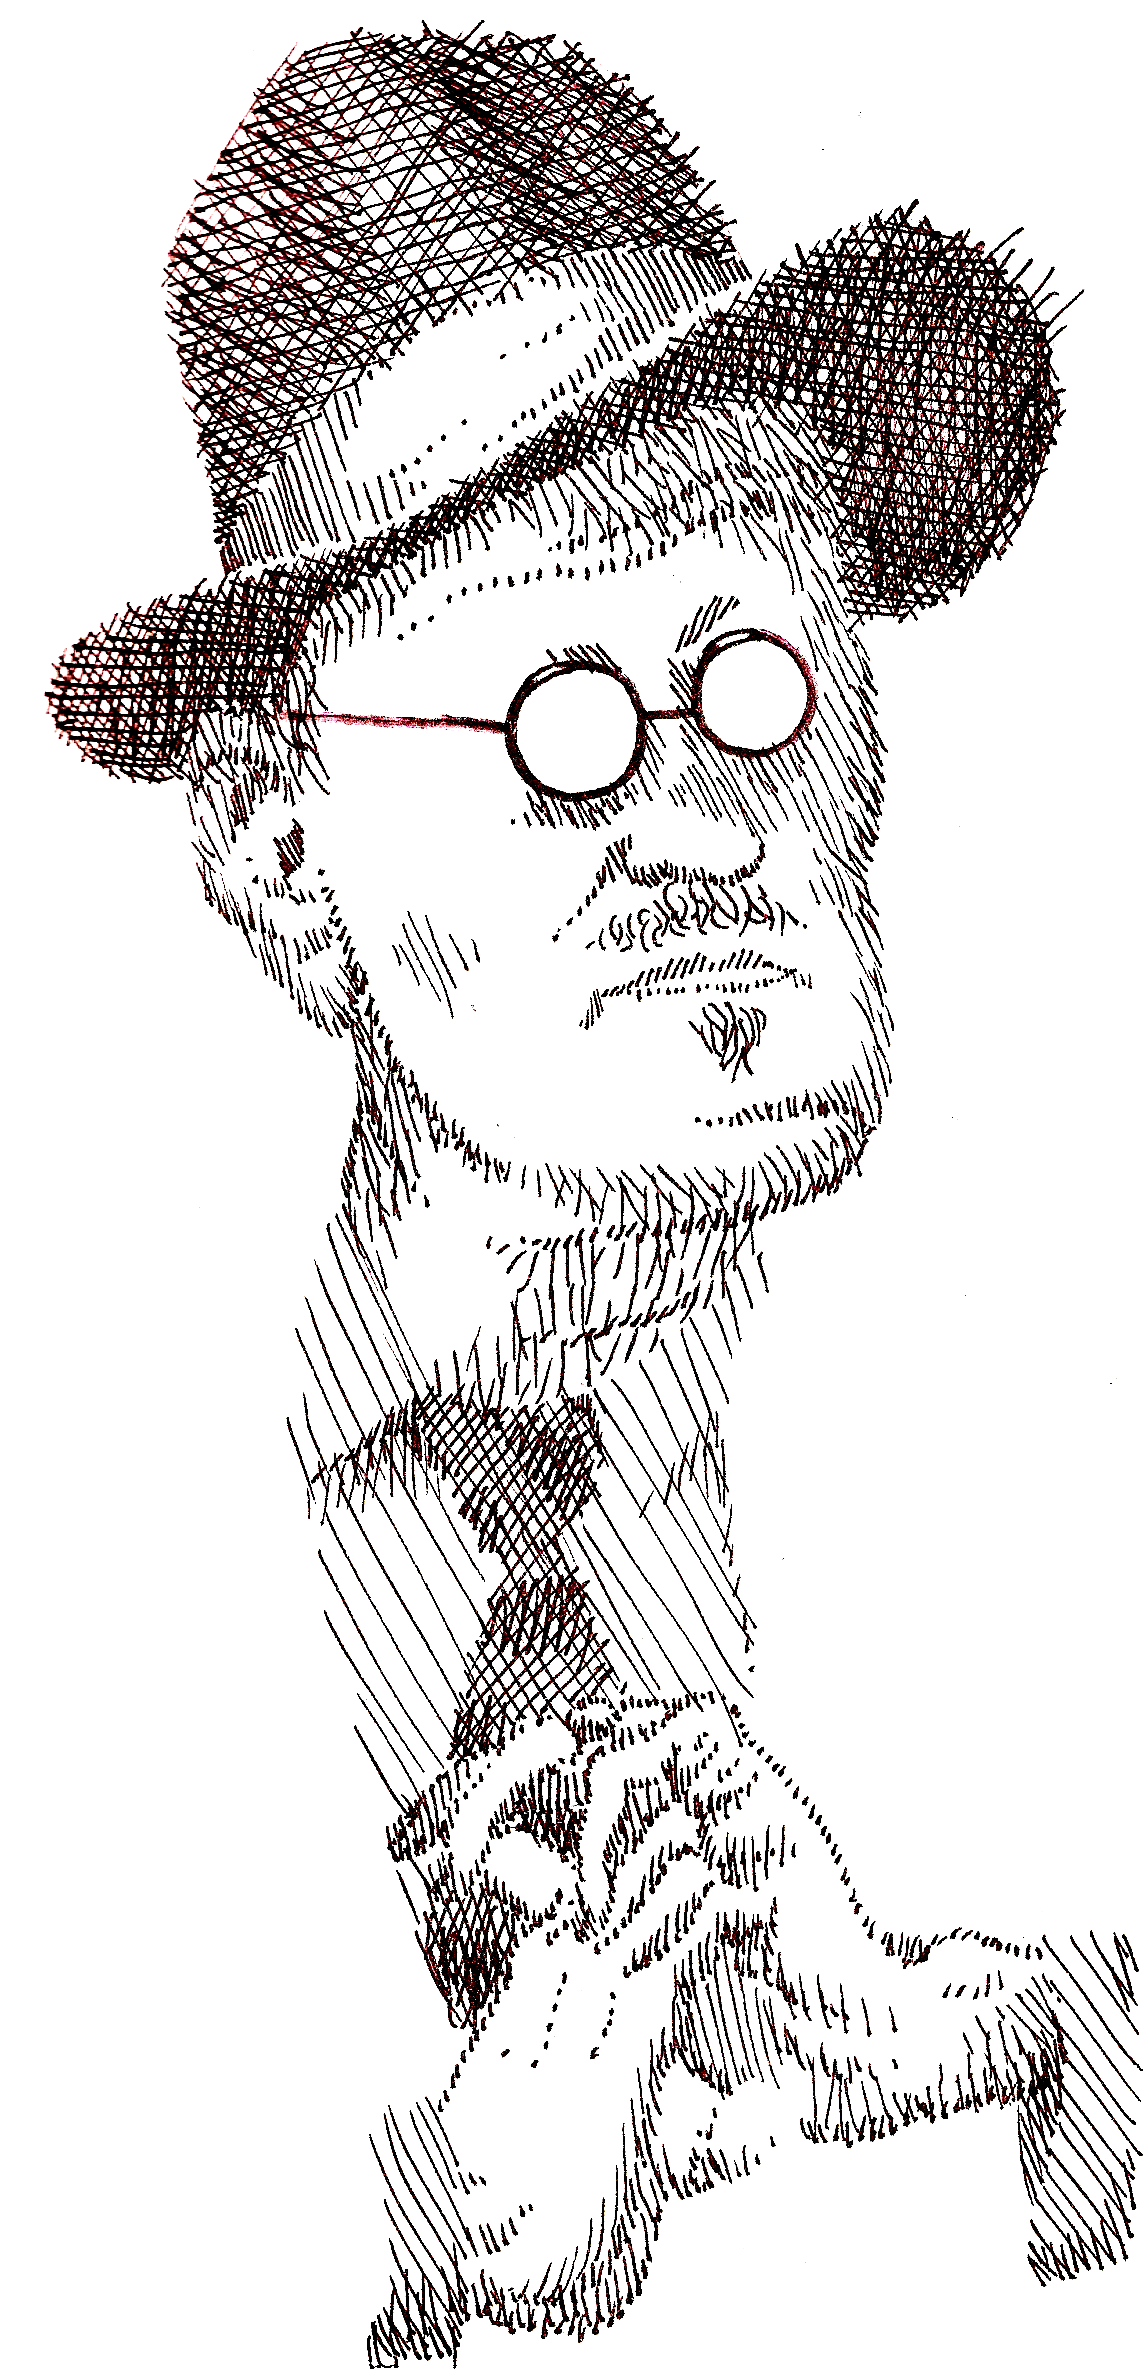
\includegraphics[width=.6\textwidth]{joyce4.jpg}
\end{center}
\end{figure}

\clearpage


\chapter*{\ } 
\markboth{Stephen Herói}{James Joyce}

{\centering
[\textit{O manuscrito inicia aqui}]
\par}
\bigskip

\noindent qualquer pessoa que falasse com ele misturava descrença exageradamente
polida e expectativa.  \label{os"-cabelos} Os cabelos crespos\endnote{ \textit{espetados}.} e castanhos eram
penteados projetando"-se da fronte mas havia pouca ordem no estilo. 
Uma jovem\endnote{ \textit{O rosto}.} talvez o considerasse atraente ou não: o rosto tinha
traços regulares com um semblante quase suavizado numa beleza com uma boca pequena e
feminina\endnote{ \textit{positiva singular}.}. Numa\endnote{ \textit{Na}.} inspeção geral do
rosto os olhos não se destacavam: eram olhos pequeninos e azuis"-claros
que desestimulavam contatos.  Eram bastante joviais e destemidos mas
apesar disso o rosto era até certo ponto o rosto de um libertino.

O reitor da universidade era uma pessoa reclusa que ocupava a
cabeceira da mesa em reuniões e cerimônias inaugurais de associações.
Seus tenentes óbvios eram um vice"-reitor e um tesoureiro.  O
tesoureiro, Stephen pensava, fazia jus ao cargo: homem obeso e corado,
com uma \label{touca"-de} touca de cabelos pretos"-grisalhos.  Realizava suas tarefas
com um entusiasmo afetado e costumava ser visto assombrando o corredor
e observando as idas e vindas dos alunos.  Insistia em pontualidade: um
minuto de atraso de vez em quando --- isso não o incomodava muito; batia
palmas e fazia alguma repreensão bem"-humorada.  Mas o que o deixava
zangado era a perda de alguns minutos todos os dias: isso perturbava o
devido andamento das aulas.  Stephen atrasava"-se quase sempre mais de
quinze minutos e quando\endnote{ \textit{portanto}.} ele chegava o tesoureiro geralmente
já havia voltado para sua sala.  Certa manhã, no entanto, ele chegou
mais cedo que de costume.  À sua frente subia os degraus de pedra um
estudante gorducho,\endnote{ \textit{jovem}.} jovem tímido e extremamente aplicado, com
uma pele cor de pão com geleia.  O tesoureiro estava de pé no corredor
com os braços cruzados diante do peito e quando viu o jovem gorducho
olhou expressivamente para o relógio.  Eram onze horas e oito minutos.

--- Então, Moloney!  Você sabe que isso não é possível.  Oito
minutos atrasado!  Perturbar a aula desse jeito\ldots{} não podemos admitir
isso, você bem sabe.  Chegue na hora certa para a aula daqui em diante.

A geleia espalhou"-se pelo pão no rosto de Moloney enquanto ele
tropeçava em desculpas acerca de um relógio atrasado e corria escada
acima diretamente para a sala de aula.  Stephen demorou"-se um pouco
pendurando o sobretudo enquanto o padre corpulento o observava
solenemente.  Então voltou a cabeça tranquilamente para o tesoureiro e
disse:

--- Bela manhã, senhor.

De imediato o tesoureiro bateu palmas e esfregou as mãos e voltou a
bater palmas.  A beleza da manhã e a exatidão do comentário afetaram"-no
ao mesmo tempo e ele respondeu alegremente:

--- Linda!  Que manhã bela e revigorante! --- e voltou a esfregar
as mãos.

Certa manhã Stephen\endnote{ \textit{ele}.} chegou três quartos de hora atrasado e
achou mais correto aguardar o início da aula de francês.  Enquanto ele
se debruçava sobre a balaustrada, esperando pela sineta do meio"-dia, um
jovem começou a subir lentamente as escadas em espiral.  A poucos
passos do patamar ele parou e voltou um rosto quadrado e rústico na
direção de Stephen.

--- Por obséquio, é por aqui que se chega à classe dos calouros?
--- ele perguntou com sotaque interiorano acentuando a primeira sílaba da
palavra calouros.

Stephen indicou"-lhe o caminho e os dois jovens começaram a
conversar.  O novo aluno chamava"-se Madden e vinha do condado de
Limerick.  Seu modo de ser, embora não fosse exatamente desconfiado,
era um tanto tímido e ele parecia grato pela atenção de Stephen.
Depois da aula de francês, os dois atravessaram juntos o parque e
Stephen levou o novato à Biblioteca Nacional.  Madden tirou o chapéu ao
passar pela catraca e no momento em que ele se inclinou sobre o balcão
para preencher a ficha do livro Stephen notou a força camponesa dos
seus maxilares.

O decano da universidade era professor de Inglês, padre Butt.  Era
considerado o homem mais competente da instituição: era filósofo e
erudito.  Tinha lido uma série de ensaios sob a égide de uma associação
em prol da abstinência total no intuito de provar que Shakespeare era
católico: tinha escrito também para refutar outro padre jesuíta que no
fim da vida convertera"-se à teoria baconiana relativa à autoria das
peças.  Padre Butt tinha sempre as mãos cheias de papéis e a batina
suja de giz.  Era como um velho galgo e seu aparelho vocal, a exemplo
das vestes, parecia estar coberto de giz.  Tinha modos cordatos para
com todos e era especialmente [\ldots{}]


\bigskip

{\centering
[\textit{Faltam duas páginas}]
\par}


\bigskip

do verso são as primeiras condições às quais as palavras devem se
submeter, sendo o ritmo o resultado estético dos sentidos, valores e
relações entre as palavras assim condicionadas.  A beleza do verso
consistia tanto no ocultamento quanto na revelação do construto mas é
certo que não podia resultar de apenas um desses fatores.  Por essa
razão ele considerava intoleráveis a leitura que padre Butt fazia de
versos e a leitura acurada que uma colegial fazia de versos.  Verso
para ser lido de acordo com o ritmo deveria ser lido de acordo com os
acentos tônicos; isto é, nem estritamente de acordo com os pés nem 
desconsiderando"-os totalmente.  Ele se dispôs a explicar toda essa teoria
a Maurice, e Maurice, ao compreender os significados dos termos e
estabelecer relações precisas entre tais significados, concordou que a
teoria de Stephen era a correta.  Só havia uma possibilidade de ler a
primeira quadra do poema de Byron:

\begin{verse}{\itshape
My dáys are in the yéllow léaf\\				
The flowers and frúits of love are góne\\			
The wórm, the cánker and the gríef\\				
Are míne alone}.\footnote{ ``Meus dias são como folhas secas/ As flores e frutos do amor tem fim/ 
O verme, o cancro e o sepulcro/ são só para mim.'' 
Os versos são exemplo de acentuação métrica em língua inglesa. O poema aludido		
é “On This Day I Complete My Thirty"-Sixth Year”
(22 de janeiro de 1824).  Na verdade, trata"-se da segunda
quadra. [N.~do~T.]}
\end{verse}

Os dois irmãos testaram essa teoria em todos os versos de que
conseguiram se lembrar e os resultados foram magníficos.  Em breve o
próprio Stephen começou a explorar a linguagem e selecionar, destarte
resgatando para sempre, as palavras e as expressões mais receptivas à
sua teoria.  \label{ele"-se} Ele se tornou um poeta prevenido e calculista.

Sentia"-se igualmente cativado pelas aparentes excentricidades da
prosa de Freeman e William Morris.  Lia esses autores como quem lesse
um tesauro e fazia um \label{celeiro} celeiro de palavras.  Lia o \textit{Dicionário
etimológico} de Skeat hora após hora e sua mente, desde sempre
demasiado submissa ao espanto típico de uma criança, costumava ficar
hipnotizada diante da conversa mais banal.  Para ele as pessoas
pareciam ignorar o valor dos vocábulos que empregavam de modo tão
superficial.  E passo a passo à medida que tal indignidade da vida lhe
era imposta ele se enamorava de uma tradição idealizada, mais
verdadeiramente humana.  O fenômeno lhe parecia importante e ele
começou a perceber que as pessoas tinham se aliado numa conspiração 
ignóbil e que com desdém o Destino tinha reduzido os preços que		
cobrava delas.  Ele não queria para si esse tipo de redução e preferia
servir ao Destino segundo as velhas condições.

Havia uma turma especial de Redação em Língua Inglesa e foi nessa
turma que Stephen primeiro se destacou.  Para ele o ensaio era o único
trabalho sério da semana.  Seu ensaio costumava ser extenso e o mestre,
redator do \textit{Freeman’s Journal}, sempre o deixava por último.  O
estilo da escrita de Stephen, embora\endnote{ \textit{que}.} por demais inclinado ao
antigo e até ao obsoleto e simploriamente retórico, era notável pela
crua originalidade de expressão.  Ele não se furtava a sustentar as
ousadias expressas ou insinuadas em seus ensaios.  Lançava"-as como
defesas inesperadas enquanto se ocupava de construir enigmas
estilísticos.  Pois o jovem tinha se dado conta da existência de uma
outra crise e queria se preparar para o impacto que ela causaria.
Devido a tais manobras, ele passou a ser visto como um jovem
desequilibrado que se interessava mais do que os jovens geralmente se
interessam por teorias que possam ser consideradas passatempo.  Padre
Butt, a quem o surgimento dessas qualidades raras tinha sido
devidamente informado, conversou com Stephen um dia com o propósito de
“sondá"-lo”.  Padre Butt expressou grande admiração pelos ensaios de
Stephen, cuja totalidade, disse ele, tinha"-lhe sido mostrada pelo
professor de Redação em Língua Inglesa.  Incentivou o jovem e sugeriu
que em breve ele talvez pudesse enviar algo para um dos jornais ou
revistas de Dublin.  Stephen considerou o incentivo bem intencionado
mas equivocado e embarcou numa eloquente explanação de suas teorias.
Padre Butt ouviu e, mais prontamente até do que Maurice,\endnote{ \textit{Stephen}.}
concordou com todas elas.  Stephen explicitou sua doutrina com bastante
convicção e insistiu na importância do que ele chamava de tradição
literária.  \label{as"-palavras} As palavras, ele disse, têm certo valor na tradição
literária e certo valor no mercado --- um valor depreciado.  As palavras
são simples receptáculos para o pensamento humano: na tradição
literária elas recebem mais pensamentos valiosos que no mercado.  Padre
Butt ouviu tudo isso, esfregando várias vezes no queixo a mão suja de
giz e, \label{meneando"-a} meneando a cabeça, disse que Stephen evidentemente compreendia a
importância da tradição.  Stephen citou uma frase de Newman para
ilustrar sua teoria.

--- Nessa sentença de Newman --- ele disse --- a palavra é
empregada segundo a tradição literária: ela tem ali o seu valor pleno.
No uso comum, isto é, no mercado, ela possui um valor totalmente
diverso, um valor depreciado.  Espero não estar detendo o senhor.

--- Absolutamente, absolutamente!

--- Não, não\ldots{}

--- Sim, sim, Mr.~Dedalus, eu entendo\ldots{} eu percebo bem o seu
ponto\ldots{} deter\ldots{}

Logo na manhã seguinte padre Butt revidou o monólogo de Stephen.  A
manhã estava fria e úmida e quando Stephen, que chegara atrasado demais
para assistir à aula de latim, entrou no anfiteatro de física e
deparou"-se com padre Butt ajoelhado diante da imensa lareira
ocupando"-se de acender um pequeno fogo.  Ele rasgava tiras de papel e
as depositava cuidadosamente entre o carvão e os gravetos.  Tagarelava
o tempo todo explicando a operação e num momento de crise retirou dos
bolsos mais remotos da batina suja de giz três tocos de vela sujos.
Enfiou os tocos de vela em diferentes aberturas e em seguida olhou para
Stephen com ar de triunfo.  Encostou um palito de fósforo nos pedaços
de papel cujas pontas se projetavam e em poucos minutos o carvão
queimava.

--- Existe arte, Mr.~Dedalus, no acendimento de um fogo.

--- É o que vejo, senhor.  Arte muito útil.

--- É isso: arte útil.  Temos as artes úteis e as artes liberais.

Depois dessa afirmação, padre Butt levantou"-se e foi cuidar de outras
tarefas deixando Stephen observar o fogo que ardia e Stephen refletiu
sobre os tocos de vela que rapidamente se derretiam e sobre a
inadequação dos modos do padre, até chegar a hora do início da aula de
física.

O problema não podia ser solucionado imediatamente, mas ao menos o
seu aspecto artístico não apresentava dificuldade.  Ao ler
\textit{Noite de Reis} para a turma, padre Butt pulou as duas canções do
bobo nada dizendo e, quando Stephen, decidido a fazer com que ele as
levasse em conta, perguntou com toda seriedade se as canções deveriam
ser memorizadas, padre Butt disse que era improvável que tal questão
surgisse na prova:

--- O bobo canta essas canções para o duque.  Era costume dos
nobres à época mandar que os bobos cantassem\ldots{} por divertimento.

Ele abordou \textit{Otelo} com mais seriedade e fez notar à turma a
moral da peça: uma lição objetiva acerca da paixão do ciúme.
Shakespeare, ele disse, sonda as profundezas da natureza humana: suas
peças nos retratam homens e mulheres sob a influência de diversas
paixões e nos apresentam a consequência moral dessas paixões.
Assistimos ao conflito dessas paixões humanas e nossas próprias paixões
são purificadas pelo espetáculo.  O teatro de Shakespeare tem uma força
moral singular e \textit{Otelo} é uma das maiores tragédias.  Stephen
se condicionou a ouvir tudo isso sem mover um dedo mas ao mesmo tempo
divertiu"-se ao saber que o diretor negara autorização a dois internos
para assistirem \label{a"-uma} a uma montagem de \textit{Otelo} no Teatro Gaiety
porque havia muitas expressões grosseiras na peça.

Ultimamente o monstro em Stephen vinha se comportando mal e à mínima
provocação mostrava"-se pronto para fazer verter sangue.  Quase todo
incidente rotineiro servia de estopim e o intelecto experimentava
grande dificuldade para mantê"-lo na linha.  Mas um episódio de fervor
religioso que rapidamente se tornava uma lembrança resultara num certo
autocontrole externo que agora se mostrava bastante útil.  Além disso
Stephen era suficientemente perspicaz para perceber a necessidade de
resolver suas questões discretamente e discrição sempre fora para ele
uma penitência leve.  Sua resistência a debater escândalos, a parecer
abelhudo e descortês, auxiliava"-o na acusação e não deixava de ter o
agradável sabor do heroico.  Já quando aquele ataque de febre de
santidade sobre ele se abatera, ele havia correspondido à altura mas
por caridade tinha declinado a penetrar forças decepcionantes.  Os
rompantes de fervor decorrentes daqueles abalos impeliram"-no
descaradamente à introversão e os exercícios da devoção tão"-somente o
confortavam.  Era um conforto do qual muito necessitava pois sofria
imensamente em consequência do contato com o novo ambiente.  Mal se
dirigia aos colegas e das tarefas acadêmicas desincumbia"-se sem
comentários ou interesse.  Todas as manhãs levantava"-se e descia para o
café.  Depois do café pegava o bonde para a cidade, sentado no primeiro
banco na parte descoberta encarando o vento.  Descia do bonde na
Estação Saint Amiens em vez de ir até Pillar porque desejava participar
da vida matinal da cidade.  Naquela manhã, a caminhada fora agradável e
não havia rosto que por ele passasse a caminho da prisão comercial que
ele não tentasse penetrar até o cerne do motivo de sua feiura.  Era
sempre com uma sensação de desprazer que ele entrava no Green e via no
outro extremo o prédio soturno da Universidade.

Enquanto seguia pelos caminhos da cidade, mantinha ouvidos e olhos
sempre atentos para registrar impressões.  Não apenas em Skeat
encontrava palavras para seu cofre"-forte, também as encontrava
aleatoriamente em lojas, anúncios, na boca da população que se
arrastava.  Ele as repetia para si mesmo até que perdessem todo
significado corriqueiro e se tornassem vocábulos fantásticos.  Estava
decidido a lutar com toda a energia do corpo e da alma contra qualquer
consignação possível em relação ao que agora considerava ser o inferno
dos infernos --- a região onde se constata que tudo é óbvio ---, e o santo
antigamente \label{discreto"-no} discreto no falar, em obediência a um voto de silêncio,
poderia ser reconhecido no artista que se condicionava ao silêncio com
receio de que as palavras lhe retribuíssem a descortesia.  Frases
chegavam até ele pedindo para serem explicadas.  Ele dizia para si
mesmo: devo esperar até que a Eucaristia venha a mim: e então se ocupou
de traduzir com bom senso essa mesma frase.  Passou dias e noites
martelando em silêncio, construindo para si a morada do silêncio onde
pudesse aguardar a Eucaristia, dias e noites colhendo os primeiros
frutos e cada regalo da paz e empilhando"-os em seu altar onde suplicava
fervorosamente pela descida de um sinal flamejante de satisfação.  Na
sala de aula, no silêncio da biblioteca, na companhia de outros alunos
ele escutava subitamente uma ordem para se retirar, para se isolar, uma
voz que lhe agitava os tímpanos, uma chama que tremulava e se
transformava numa divina vida cerebral.  Obedecia à ordem e perambulava
pelas ruas sozinho, com o fervor da esperança sustentado por
ejaculações até se certificar de que era inútil continuar perambulando:
e então voltava para casa com passadas resolutas, incansáveis,
costurando palavras e frases desconexas com uma seriedade resoluta e
incansável.\footnote{ No manuscrito, aparece grafado em lápis vermelho “Final
do Primeiro Episódio de \textsc{v}”. [Nota do editor original, doravante indicada por N.~do~E.]}


\section{XVI}

Suas Eminências do Santo Colégio não eram mais zelosas e solitárias
durante a eleição do vigário de Cristo que Stephen àquela época.  Ele
escreveu muito verso e, na falta de um instrumento mais adequado, o
verso permitia"-lhe combinar os ofícios de penitente e confessor.  Nos
versos ele procurava fixar o seu estado de espírito mais inescrutável e
suas linhas não eram compostas palavra por palavra mas letra por letra.
Leu Blake e Rimbaud acerca dos valores das letras e chegou a permutar
e combinar as cinco vogais a fim de construir clamores que invocassem
emoções primitivas.  A nenhum dos antigos fervores ele se entregara com
tamanha devoção como no caso desse fervor; \label{o"-monge} o monge agora não lhe
parecia ser mais que um meio artista.  Convenceu"-se de que o artista
precisava trabalhar incessantemente a sua arte se desejasse expressar
plenamente a mais simples das concepções e acreditava que cada momento
de inspiração requeria pagamento antecipado.  Tinha dúvidas quanto à
veracidade do provérbio “O poeta nasce, não é feito” mas tinha
certeza\endnote{ \textit{Poeta nascitur, non fit}.} ao menos quanto à veracidade do
seguinte: “O poema é feito, não nasce”.\endnote{ \textit{Poema fit, non nascitur}.}
A noção urbana do poeta Byron despido vertendo versos
qual\endnote{ \textit{como}.} uma fonte municipal verte água parecia"-lhe típica da maioria das
avaliações populares acerca de questões estéticas e ele combatia tal
noção em sua raiz \label{dizendo"-solenemente} dizendo solenemente a Maurice --- o isolamento é o
primeiro princípio da economia artística.

Stephen não se apegava à arte com qualquer espírito de diletantismo
jovial mas buscava penetrar o coração significativo de tudo.
\label{mergulhava"-no} Mergulhava no passado da humanidade e vislumbrava a arte emergente
como quem tem a visão de um plesiossauro emergindo de um mar de lodo.
Parecia ouvir os gritos de medo e alegria e espanto que
antecedem de todas as canções, e os ritmos selvagens de homens
remando, parecia enxergar os rabiscos toscos e os deuses portáteis de
homens cujo legado coube a Leonardo e Michelangelo.  E acima de todo
esse caos de história e mito, fato e suposição, ele tentou traçar uma
linha de ordem, tentou reduzir à ordem os abismos do passado por meio
de um diagrama.  Os tratados que lhe foram recomendados mostraram"-se
inúteis e superficiais; o \textit{Laocoonte} de Lessing o irritava.
Perguntava"-se como o mundo era capaz de aceitar como contribuições
valiosas generalizações assim tão fantásticas.  Que certeza mais
significativa poderá o artista obter se acreditar que a arte antiga era
plástica e a moderna pictórica --- arte antiga nesse contexto significa
arte produzida entre os Bálcãs e a Moreia e arte moderna significa arte
produzida entre o Cáucaso e o Atlântico, exceto na região sacrossanta.
Era devorado por grande desprezo por críticos que consideravam “grego”
e “clássico” termos sinônimos e ficava tomado por uma raiva tão
incontrolada que quando\endnote{ \textit{a semana toda sábado}.} padre Butt designou
\textit{Otelo} como tema do ensaio semanal, Stephen entregou na
segunda"-feira seguinte um copioso manifesto contra a “obra"-prima”.  Os
rapazes da turma riram e Stephen, olhando com desprezo as caras
risonhas, pensou num réptil autossubmergível.

Ninguém dava ouvidos às suas teorias: ninguém se interessava por
arte.  Os \label{colegas} colegas encaravam a arte como um vício continental e, com
efeito, diziam “Se precisamos de arte, não haverá temas suficientes nas
Sagradas Escrituras?” --- pois artista, para eles, era um indivíduo
que pintava quadros.  Era mau sinal um jovem demonstrar interesse por
algo além dos exames ou do futuro “emprego”.  Era aceitável falar sobre
o assunto, mas na realidade arte era só “bobagem”: além disso era
provavelmente imoral; eles tinham conhecimento (ou, ao menos, ouviram
falar) de estúdios.  Não queriam esse tipo de coisa em seu país.  Em se
tratando de beleza, em se tratando de ritmos, em se tratando de
estética --- eles sabiam o que esses belos tópicos abrangiam.  Um dia
um aluno grandalhão e interiorano aproximou"-se de Stephen e perguntou:

--- \label{diga"-nos} Diga"-nos, você não é artista?

Stephen fitou o jovem imune a ideias, sem responder.

--- Se você é, por que não tem cabelo comprido?

Algumas pessoas em volta riram e Stephen se perguntou qual profissão		
culta o pai do jovem teria escolhido para o filho.

A despeito do ambiente Stephen prosseguiu com as pesquisas e o fez
com mais afinco pois imaginava que suas investigações tinham sido
\label{proscritas} proscritas.  Devido àquele egoísmo inerradicável que mais tarde		
chamaria de redentor, ele supunha que os feitos e os pensamentos do seu
microcosmo a ele convergissem.  Será medieval a mente da juventude por
ser tão sensível à intriga?  Os divertimentos do campo (ou seu
equivalente no mundo da mentalidade) talvez sejam a cura mais eficaz e
os educadores anglo"-saxônicos favorecem um sistema de ousada
brutalidade.  Mas para o idealista fantástico, esquivando"-se com um
salto da aparição que grunhe, o combate mímico não terá sido menos
ridículo que desigual num terreno escolhido para prejudicá"-lo.  Detrás
do rígido escudo, o sensível respondeu: que o bando de inimizades,
saltando e farejando, venha até as minhas montanhas na perseguição da
caça.  Ali era o terreno dele e ele dispensou"-lhes desdém com seus
chifres reluzentes.\footnote{ Essa frase ocorre no poema satírico de
Joyce, “The Holy Office” (“O Santo Ofício”). [N.~do~E.]}		

Deveras ele sentia a manhã no sangue: tinha percebido um movimento
já procedente \label{na"-europa} na Europa.  Essa última frase lhe agradava porque
parecia expor o mundo mensurável aos pés dos ilhéus.  Nada era capaz de
convencê"-lo de que o mundo correspondesse à concepção dos alunos do
padre Butt.  Ele não precisava dos cuidados identificados como
indispensáveis, tampouco demonstrava reverência pelos escrúpulos
rotulados como a base da vida.  Era uma figura enigmática em meio a uma
sociedade fragmentada na qual gozava de reputação.  Seus companheiros
mal sabiam até que ponto podiam com ele se aventurar e os professores
fingiam achar que a seriedade dele era garantia suficiente contra
qualquer desobediência prática.  Da parte dele, a castidade, provando
constituir um grande inconveniente, tinha sido abandonada com discrição
e o jovem se divertia na companhia de alguns colegas dos quais (segundo
corria a fama) a vida desregrada não era desconhecida.  O reitor de
Belvedere tinha um irmão que àquela época estudava na universidade e
certa noite, na galeria do Gaiety (Stephen se tornara um “deus”
frequente), outro rapaz de Belvedere, \label{que"-tambem} que também estudava na
universidade, levou um testemunho escandaloso aos ouvidos de Stephen.

--- Escute aqui, Dedalus\ldots{}

--- Sim?

--- O que o MacNally diria se encontrasse o irmão\ldots{} você sabe, o
cara que estuda na universidade?

--- Sim\ldots{}

--- Eu o vi o outro dia no Stephen’s Green com uma prostituta.
Eu estava imaginando\ldots{} se o MacNally o visse\ldots{}

O informante fez uma pausa: e então, com receio de se envolver
demais e com um ar de especialista, acrescentou, falando seriamente:

--- É claro que ela era\ldots{} tudo bem.

Todas as noites depois do chá Stephen saía de casa e se dirigia à
cidade, acompanhado de Maurice.  O mais velho fumava cigarros e o mais
jovem chupava dropes de limão e, animados por esses lenitivos sensuais,
entretinham a longa caminhada com discurso filosófico.  Maurice era
pessoa bastante atenciosa e certa noite disse a Stephen que estava
escrevendo um diário que registrava as conversas dos dois.  Stephen
pediu para ver o diário mas Maurice disse que haveria tempo suficiente
para tal ao término do primeiro ano.  Nenhum dos dois jovens
desconfiava do outro; ambos contemplavam a vida com olhos sinceros e
curiosos (Maurice naturalmente servia"-se da visão de Stephen quando a
sua era deficiente) e ambos achavam ser possível chegar a um
entendimento saudável dos chamados mistérios desde que se tivesse a
paciência necessária.  Todas as noites em suas caminhadas eles cruzavam
os píncaros do debate e o mais jovem colaborava com o mais velho
bravamente na construção de uma completa ciência estética.  Conversavam
com grande determinação e Stephen considerava Maurice muito útil quando
este levantava objeções.  Chegando ao portão da biblioteca, costumavam
se deter a fim de concluir algum ponto relativo ao assunto e com
frequência a discussão tanto se prolongava que Stephen resolvia ser
tarde demais para entrar e ler e então dirigiam"-se a Clontarf e
voltavam do mesmo modo.  Stephen, após certa hesitação, mostrou a
Maurice os primeiros frutos do seu verso e Maurice perguntou quem era a
mulher.  Stephen olhou adiante um tanto vagamente antes de responder e
por fim teve de dizer que não sabia quem ela era.

Para essa desconhecida versos eram agora compostos regularmente e
parecia que o sonho malévolo do amor que Stephen comemorava em tais
versos impunha"-se verdadeiramente ao mundo numa estação de \label{nevoa"-umida} névoa úmida
e violeta.  Ele abandonara sua Madona, descumprira a própria palavra e
se retirara implacavelmente do seu mundinho e com certeza não era
magnífico que a solidão o impelisse aos rompantes frenéticos da paixão
juvenil e do isolamento.  Essa característica da mente que assim se
revela é chamada (quando incorrigível) de decadência, mas se quisermos
ter uma visão geral do\endnote{ \textit{da vida}.} mundo não podemos deixar de ver no
declínio um processo de vida.  Havia para ele, no entanto, momentos em
que tal processo parecia intolerável, a vida, em quaisquer termos
comuns, uma ofensa intolerável, e nesses momentos ele por nada rezava e
de nada se lamentava mas sentia com um agradável peso na consciência
que se o fim a ele chegasse isso ocorreria nos braços da desconhecida:

\begin{verse}
Desperta a aurora com trêmulo alarde,\\
\hspace*{2em} Que cinzenta, que lúgubre, que gelo!\\
Ó, envolve"-me braço alvo, braço que arde!\\
\hspace*{2em} E esconde"-me, copioso cabelo!

A vida é sonho, sonho. Passa a hora\\
\hspace*{2em} E a antífona já soou forte.\\
Da luz e da fraude do sol agora\\
\hspace*{2em} Passamos à triste ruína da morte.
\end{verse}

Pouco a pouco Stephen se tornou menos assíduo na universidade.
Costumava sair de casa todas as manhãs no mesmo horário e pegava o
bonde para a cidade.  Mas sempre descia na estação de Amiens e
caminhava e sempre resolvia seguir algum indício banal da vida urbana
em vez de adentrar a vida opressiva da universidade.  Caminhava durante
sete ou oito horas sem parar e não sentia o menor cansaço.  O úmido
inverno dublinense parecia se harmonizar com sua lassidão interior e
ele não seguia por caminhos tortuosos, inesperados, a menor das
provocações femininas, assim como não seguia por caminhos ainda menos
gratificantes os movimentos lépidos da desconhecida.  Como seria Ela:
braços de amor desprovidos da crueldade do amor, riso correndo pelas
montanhas da manhã, numa hora em que o incomunicável pudesse ser
encontrado?  E se o coração tremesse um instante, ele gritava,
jovialmente, apaixonadamente: “É isso!  É isso!  A vida é como eu a
concebo”.  Tirou da frente as máximas rançosas dos jesuítas e jurou
que estas jamais exerceriam sobre ele qualquer ascendência.  Tirou da
frente o mundo da cultura esnobe no qual não existia erudição nem arte
nem dignidade de gestos --- um mundo de intrigas banais e triunfos
banais.  Acima de tudo tirou da frente a companhia de jovens
decrépitos --- e jurou que estes jamais firmariam com ele qualquer
pacto fraudulento.  Belas palavras!  Belos juramentos!  Brados valentes
e apaixonados, mesmo no calor das circunstâncias.  Pois não raro nas
pausas daquele arroubo Dublin tocava"-lhe subitamente o ombro, \label{e"-a} e a
frieza do chamado penetrava"-lhe o coração.  Certa vez, a caminho de casa,
passou por Fairview.  Numa bifurcação da estrada diante da praia
alagadiça um grande cão estava deitado.  De vez em quando ele erguia o
focinho no ar nevoento, emitindo um uivo longo e melancólico.  Algumas
pessoas se juntaram nas trilhas para ouvi"-lo. Stephen\endnote{ \textit{e}.} emitiu um uivo
até sentir as primeiras gotas de chuva, e então prosseguiu em silêncio
sob a morosa vigilância do céu, ouvindo de vez em quando, atrás de si,
o estranho lamento.

Era natural que quanto mais o jovem buscava a solidão tanto mais as
companhias buscavam frustrar"-lhe o propósito.  Embora ainda estivesse
no primeiro ano, já era considerado uma personalidade e muitos pensavam
que apesar de um pouco exacerbadas suas teorias não eram desprovidas de
sentido.  Stephen raramente assistia às aulas, não apresentava trabalho
algum e não comparecia aos exames finais, mas não apenas nada se dizia a
respeito de tais extravagâncias como também se supunha que ele deveras
representasse o tipo artístico que ele, de fato, era e que, conforme o
hábito dessa tribo desconhecida, praticasse o autodidatismo.  Não se
deve supor que a conhecida Universidade da Irlanda carecesse de um
centro inteligente.  Fora do grupo compacto de nacionalistas
\label{pregadores"-havia} pregadores havia aqui e ali estudantes com certas ideias próprias e
que eram mais ou menos tolerados pelos colegas.  Por exemplo, havia um
jovem e sério feminista chamado McCann --- figura franca e vivaz, com
sua barba de mosqueteiro e seu traje de caça, leitor ferrenho da
\textit{Review of Reviews}.  Os alunos da universidade não compreendiam
o tipo de ideias que ele abraçava e achavam que compensavam a contento
a originalidade do rapaz chamando"-o de “Knickerbockers”.\footnote{
Calção folgado, preso um pouco abaixo dos joelhos, usado à época como
traje de caça. [N.~do~T.]}  Havia também o orador da universidade ---
jovem extremamente amável que discursava em todas as reuniões.  Cranly
também era uma personalidade e Madden foi logo reconhecido como o
\label{porta"-voz} porta"-voz do partido patriótico.  Pode"-se dizer que Stephen ocupava a
posição do notável"-excêntrico: poucos tinham ouvido falar nos autores
que, segundo corria, ele costumava ler e os que tinham ouvido falar em
tais autores consideravam"-nos insanos.  Ao mesmo tempo em que a conduta
de Stephen a todos parecia inflexível supunha"-se que ele houvesse
preservado a sanidade e que resistisse bravamente às tentações.  As
pessoas começaram a acatá"-lo, a convidá"-lo às suas casas e a
dirigir"-lhe semblantes graves.  O que ele advogava eram simplesmente	
teorias e, de vez que ainda não infringira qualquer lei, foi
respeitosamente convidado a ler um ensaio diante da Associação
Literária e Histórica da Universidade.  Fixou"-se a data no fim de março
e o título do ensaio foi anunciado como “Drama e vida”.  Muitos se
submetiam ao risco de ser ignorados na tentativa de puxar conversa com
o jovem excêntrico mas Stephen guardava um silêncio desdenhoso.  Certa
vez, enquanto ele voltava de uma festa um repórter de um dos jornais de
Dublin, que tinha sido apresentado ao prodígio naquela mesma noite,
abordou"-o e após algumas palavras disse"-lhe tentativamente:

--- Estive lendo aquele autor\ldots{} como é mesmo que o senhor o
chama\ldots{} Maeterlinck\ldots{} um dia desses\ldots{} sabe?		

--- Sim\ldots{}

--- Estive lendo\ldots{} \textit{O intruso}\ldots{} acho que era esse o
título\ldots{} peça\ldots{} muito estranha\ldots{}

Stephen não queria falar com o sujeito sobre Maeterlinck, mas por
outro lado desagradava"-lhe a ideia de ofendê"-lo com o silêncio que o
comentário, o tom e a intenção mereciam, portanto vasculhou por um
instante a mente em busca de alguma banalidade que não o comprometesse
e com a qual pudesse se livrar da dívida.  Finalmente, disse:

--- Seria difícil encená"-la.

O jornalista ficou bastante satisfeito com a troca de ideias como se
essa fosse a única impressão que a peça de Maeterlinck lhe causara.
Assentiu com convicção:

--- Ah, sim!\ldots{} Praticamente impossível\ldots{}

Referências dessa natureza a algo que lhe era tão caro magoavam
Stephen profundamente.  É preciso que se diga direta e imediatamente
que àquela época Stephen sofreu a influência que mais lhe marcou a
vida.  O espetáculo do mundo conforme apresentado por sua inteligência
com todos os detalhes sórdidos e enganosos alinhado ao espetáculo do
mundo apresentado pelo monstro que o habitava, agora guindado a um
estágio razoavelmente heroico, também costumava levá"-lo a um desespero
tão súbito que só podia ser aplacado por meio da composição de versos
melancólicos.  Estava prestes a considerar os dois mundos alheios entre
si --- por mais dissimulados que fossem ou por mais que expressassem o
mais completo pessimismo ---, quando encontrou, valendo"-se de
traduções pouco procuradas, o espírito de Henrik Ibsen.  Compreendeu		
tal espírito \label{instantaneamente} instantaneamente.  Alguns anos antes esse mesmo tipo de
entendimento instantâneo já havia ocorrido quando ele lera um relato
confuso, apologético, do biógrafo inglês de Rousseau, um relato segundo		
o qual o \label{jovem"-filosofo} jovem filósofo roubara colheres da amante e permitira que
uma criada fosse acusada do furto exatamente no momento em que Rousseau
iniciava a luta em nome da Verdade e da Liberdade.  O que ocorrera com
o filósofo perverso\endnote{ \textit{pervertido}.} agora se repetia: Ibsen não precisava
de defensor ou de crítico: as mentes do velho poeta nórdico e do jovem
celta inquieto se encontravam num momento de radiante simultaneidade.
Stephen foi cativado primeiramente pela nítida excelência da arte: não
demorou muito para ele afirmar, mesmo com escasso conhecimento do
tratado, obviamente, que Ibsen era o melhor dramaturgo do mundo.  Em
traduções dos teatros hindu ou grego ou chinês ele detectava
tão"-somente presságios ou tentativas e no teatro clássico francês, e no
teatro romântico inglês, os presságios eram menos marcantes e as
tentativas menos bem"-sucedidas.  Mas não era apenas essa excelência que
o cativara: não era isso que ele saudava com satisfação, um saudar
plenamente jubiloso e espiritual.  Era o espírito do próprio Ibsen cuja
movimentação surgia discernível detrás do estilo impessoal do
artista:\endnote{ \textit{Ibsen com sua profunda autoaprovação, Ibsen com sua coragem altiva e
desiludida, Ibsen com sua energia minuciosa e voluntariosa}.}
uma mente dotada de bravura sincera e juvenil, de orgulho desiludido, de energia
minuciosa e voluntariosa.\footnote{ A revisão aparece escrita a lápis,
na margem, talvez inserida em data posterior àquela do manuscrito. [N.~do~E.]}  
Que o mundo se resolva conforme lhe aprouver, que o suposto
Criador se justifique recorrendo aos processos que lhe convierem, mal
se pode avançar com a dignidade da atitude humana um passo sequer além
dessa resposta.  Ali e não em Shakespeare ou Goethe estava o sucessor
do primeiro poeta dos europeus, ali, somente como em Dante, uma
personalidade humana se unira a um estilo artístico que em si mesmo
constituía quase um fenômeno natural: e o espírito da época promovia
uma união mais imediata com o norueguês que com o florentino.

Os jovens da universidade não faziam a menor ideia de quem era Ibsen
mas com base no que ouviam aqui e ali deduziram que ele seria um dos
\label{escritores"-ateus} escritores ateus listados pelo secretário do papa no \textit{Index}.
Era raro ouvir alguém pronunciar tal nome na universidade e como os
professores não forneciam qualquer diretriz acerca da condenação os
alunos concluíram que seria melhor aguardar.  Nesse ínterim
mostravam"-se bastante impressionados: muitos passaram a dizer que,
embora imoral, Ibsen era um grande autor e alguém ouviu um dos
professores dizer que, gozando férias em Berlim, no verão anterior,
constatara que muito se comentava sobre uma peça de Ibsen que estava em
cartaz num teatro local.  Stephen começara a estudar dinamarquês em vez
de se preparar para os exames e tal fato foi aumentado e transformado
no relato de que ele era um competente estudioso do idioma.  O jovem
era suficientemente astuto para se beneficiar de boatos cujo conteúdo
não se preocupava em negar.  Sorria ao pensar que tais pessoas no fundo
receassem que ele fosse pagão e admirava a qualidade de suas supostas
crenças.  Padre Butt conversava bastante com ele e Stephen não relutava
em \label{se"-fazer} se fazer passar por arauto de uma nova ordem.  Jamais falava de
maneira exaltada e sempre argumentava como se pouco lhe importasse o
resultado do debate, ao mesmo tempo em que jamais perdia uma questão.
Os jesuítas e seus rebanhos talvez dissessem entre si: o \label{jovem"-aparentemente} jovem
aparentemente independente nós já conhecemos, e o patriota apaziguado
nós já conhecemos, mas quem é você?  Saíam"-se bem na tentativa de
alcançá"-lo, \label{considerando"-suas} considerando suas desvantagens, e Stephen não conseguia
entender por que todos se esforçavam para agradá"-lo.

--- Sim, sim --- disse padre Butt certa vez depois de uma dessas
cenas --- eu entendo\ldots{} eu entendo muito bem o seu argumento\ldots{} isso se
aplica evidentemente aos dramas de Turguêniev?

Stephen tinha lido e admirado algumas traduções de romances e contos
de Turguêniev e portanto indagou num tom de voz sincero:

--- O senhor quer dizer aos romances?

--- Romances, sim --- disse padre Butt imediatamente --- romances, é
claro\ldots{} mas são dramas\ldots{} não são, Mr.~Dedalus?

Stephen visitava frequentemente uma casa em Donnybrook cuja
atmosfera se mostrava plena de patriotismo liberal e estudo ortodoxo.
Havia na família várias filhas em idade de se casar e sempre que uma
promessa era sinalizada por algum jovem estudante ele era convidado à
referida casa.  O jovem feminista McCann era visitante assíduo e Madden
aparecia ocasionalmente.  O pai era um senhor idoso que jogava xadrez à
noite durante a semana com os filhos adultos e participava de jogos e
saraus nas noites de domingo.  A música ficava a cargo de Stephen.
Havia na sala um velho piano e, quando o salão se cansava dos jogos, uma
das filhas tinha o hábito de se aproximar sorrindo de Stephen e
\label{pedir"-lhe"-que} pedir"-lhe que cantasse uma de suas belas canções.  As teclas do piano
estavam gastas e às vezes as notas não soavam, mas o tom era suave e
doce e Stephen costumava sentar"-se e cantar belas canções diante da
plateia educada, cansada e pouco musical.\footnote{ As palavras
“relutava em partir” aparecem escritas a lápis vermelho, na margem, ao
lado dessas frases. [N.~do~E.]}  As canções, a menos para ele, eram		
deveras belas --- velhas cantigas do interior da Inglaterra e elegantes
cantos elisabetanos.  A “moral” dessas canções era por vezes um tanto
dúbia e os ouvidos de Stephen logo captavam a nota de restrição no
aplauso que as seguia.  As filhas bem"-intencionadas consideravam tais
canções bastante graciosas mas Mr.~Daniel dizia que Stephen deveria
cantar ópera se quisesse que sua voz fosse ouvida adequadamente.  A
despeito da total falta de sintonia em relação ao referido círculo,
Stephen ficava bem à vontade ali e sentia"-se, conforme lhe era instado,		
“em casa”, sentado no sofá, contando as protuberâncias de crina de
cavalo com as pontas dos \label{dedos"-e} dedos, e escutando as conversas.  Os jovens
e as filhas se divertiam bastante sob o olhar de Mr.~Daniel, mas sempre
que durante os jogos eram abordadas questões artísticas Stephen, com um
humor egoísta, imaginava que sua presença fosse sinal de boa conduta.
Ele pôde constatar um ar de seriedade estampado no semblante
inteligente de um jovem que dirigira uma pergunta a uma das filhas:

--- Acho que agora é a minha vez\ldots{}  Bem\ldots{} deixe"-me ver --- e aqui
ele ficou tão sério quanto possível a um jovem que acabara de rir
durante cinco minutos --- Quem é o seu poeta predileto, Annie?

Annie pensou durante alguns instantes: seguiu"-se uma pausa.  Annie e
o jovem estavam “fazendo” o mesmo curso.

--- \ldots{} Alemão?

--- \ldots{} Sim.

Annie pensou durante mais alguns instantes enquanto a mesa aguardava
para ser esclarecida.

--- Eu acho\ldots{} Goethe.

McCann tinha o hábito de organizar \label{jogos"-de} jogos de dramatização\break nos quais
costumava assumir os papéis mais intensos.  Os jogos eram extremamente
farsescos e todos assumiam de boa vontade seus papéis, tanto Stephen
quanto os demais.  Stephen fazia\endnote{ \textit{frequentemente}.} contrastar o seu
estilo discreto e reflexivo com a atuação fogosa de McCann, e por isso
os dois eram muitas vezes “escolhidos” para competir.  Tais jogos
cansavam Stephen um pouco, mas McCann se aprazia em organizá"-los pois
achava que o divertimento era necessário para o bem"-estar físico da
humanidade.  O sotaque nortenho do jovem feminista sempre provocava
risos e seu rosto, enfeitado pela barba de mosqueteiro, era
perfeitamente capaz de produzir as caretas mais descaradas.  Na
universidade McCann jamais\endnote{ \textit{foi}.} fora aceito devido às suas “ideias”,
mas ali ele participava da intimidade da família.\footnote{ Ao lado
deste parágrafo, as palavras “baile de traje a rigor: Emma” aparecem
escritas a lápis vermelho. [N.~do~E.]}  Naquela casa era costumeiro chamar		
um visitante jovem \label{pelo"-seu} pelo seu primeiro nome um pouco cedo demais e,
embora Stephen fosse poupado de tal cortesia, McCann jamais era chamado
de outro nome que não fosse “Phil”.  Stephen costumava chamá"-lo de
“Bonny Dundee”, ilogicamente associando seu\endnote{ \textit{o}.} nome exuberante e suas
\label{maneiras"-exuberantes} maneiras exuberantes com o som do verso:

\begin{verse}{\itshape
Come fill up my cup, come fill up my can.}\footnote{
Isto é: “Vem encher minha taça, vem encher minha lata”.  As palavras
“\textit{fill}” e “\textit{my can}”, em sua enunciação, reproduzem o
nome e o sobrenome do personagem. [N.~do~T.]}
\end{verse}

Sempre que a noite adquiria ares de seriedade Mr.~Daniel era
requisitado a declamar algo para os convidados.  Mr.~Daniel fora
gerente de um teatro em Wexford e tinha \label{falado"-em} falado em público por todo o
país.  Recitava textos nacionalistas com um estilo grave, declamatório,
em meio a um silêncio atento.  As filhas também declamavam.  Durante
tais recitações o olhar de Stephen jamais se afastava da estampa do
Sagrado Coração pendurada logo acima da cabeça do declamador.  As irmãs
Daniel não eram tão imponentes quanto o pai e seus vestidos
[\textit{palavra riscada, ao ponto de se tornar ilegível}] um tanto
\textit{colleen}.\footnote{ Isto é, os vestidos eram tipicamente
irlandeses.  A palavra irlandesa \textit{cailin} significa menina, não
raro com conotação de “interiorana” (o tradutor agradece o
esclarecimento ao professor Weldon Thornton). [N.~do~T.]}  \label{jesus} Jesus, além
do mais, expunha seu coração de maneira demasiado explícita na estampa
barata: e os pensamentos de Stephen eram propensos a se deixar fascinar
por essa dupla de futilidades, levando"-o a um agradável estupor.  Um
jogo que invocava o parlamento era frequente.  Mr.~Daniel havia
representado seu condado de origem anos antes e por isso era escolhido
para o papel de Presidente da Câmara.  McCann sempre atuava como
parlamentar da Oposição e falava com franqueza.  Então outro
parlamentar protestava e seguia"-se uma simulação de procedimentos
parlamentares.

--- Senhor Presidente, devo indagar\ldots{}

--- Ordem!  Ordem!

--- Vossa Excelência sabe que isso é mentira!

--- Vossa Excelência deve se retirar.

--- Conforme eu dizia quando o ilustre cavalheiro me interrompeu,
nós devemos\ldots{}

--- Não vou me retirar.

--- Peço aos ilustres parlamentares que preservem a ordem na
Câmara.

--- Não vou me retirar.

--- Ordem!  Ordem!

Outro jogo preferido era “Quem é quem”.  Uma pessoa saía da sala e
os presentes escolhiam o nome de alguém que supostamente sentisse certa
simpatia pelo participante ausente.  Este, ao retornar ao grupo,
formulava perguntas a cada um dos presentes e tentava adivinhar o nome.
O jogo costumava desconcertar os jovens convidados pois a maneira como
era conduzido sugeria que cada estudante tinha algum envolvimento
sentimental com alguma jovem que se encontrava bastante próxima dele:
mas os jovens, inicialmente surpresos com as insinuações, acabavam
dando a impressão de achar que a sagacidade dos demais participantes
lhes antecipara descobertas inesperadas, mas não desagradáveis.  O
grupo não tinha como fazer esse tipo de insinuação no caso de Stephen e
portanto na primeira vez que ele participou, a escolha do nome foi
feita de modo diferente.  Os participantes\endnote{ \textit{o grupo}.} não responderam às
perguntas por ele formuladas ao voltar à sala: perguntas tais como:
“Onde mora essa pessoa?”, “A pessoa é casada ou solteira?”, “Qual é a
idade dessa pessoa?” só puderam ser respondidas depois que McCann foi
consultado à meia voz.  A resposta “Noruega” forneceu imediatamente a
pista que Stephen precisava e assim o jogo terminou e o grupo voltou a
se divertir conforme se divertiam antes daquela séria interrupção.
Stephen sentou"-se ao lado de uma das filhas e, embora admirasse a graça
rural de seus traços, permaneceu calado na expectativa de ouvir a
primeira palavra da jovem, que, ele bem sabia, acabaria com sua
satisfação.  Seus olhos belos e grandes olharam"-no durante alguns
instantes como se estivessem \label{prestes"-a} prestes a nele confiar e então ela
disse:

--- Como você adivinhou tão depressa?

--- Eu sabia que você estava pensando nele.  Mas você está
enganada em relação à idade.

Os demais ouviram isso: mas ela ficou impressionada com a amplitude
do desconhecimento, lisonjeada por trocar ideias com alguém que
interagia diretamente com o excepcional.  Inclinou"-se para falar com
uma seriedade meiga:

--- Ora!  Quantos anos ele tem?

--- Mais de setenta.

--- É mesmo?

Stephen agora achava que já havia explorado o local suficientemente
e teria suspendido as visitas se dois motivos não o induzissem a
perseverar.  O primeiro motivo foi a natureza desagradável do seu
próprio lar e o segundo foi a curiosidade suscitada pelo advento de uma
nova figura.  Certa noite, enquanto meditava no sofá de crina de cavalo,
ele ouviu seu nome ser chamado e levantou"-se para ser apresentado a
alguém.  Uma jovem morena \label{desenvolvida} desenvolvida estava de pé diante dele e,
sem esperar que Miss Daniel o apresentasse, disse:

--- Acho que já nos conhecemos.

Ela sentou"-se ao lado dele no sofá e ele ficou sabendo que ela estudava
na mesma instituição que as irmãs Daniel e que sempre assinava o
próprio nome em irlandês.  Disse que Stephen deveria \label{aprender"-irlandes} aprender irlandês
também e se filiar à Liga.  Um jovem ali presente, cujo\endnote{ \textit{com}.}
semblante exibia sempre o mesmo ar estudado de determinação, dirigiu"-se
a ela, falando por cima de Stephen, chamando"-a com intimidade pelo nome
irlandês.  Stephen por conseguinte falou com toda formalidade e fez
questão de chamá"-la de “Miss Clery”.  Por seu turno, ela parecia
incluí"-lo no \label{esquema"-geral} esquema geral do seu charme nacionalizante: e quando ele
a ajudou a vestir o casaco ela deixou que as mãos dele tocassem um
instante a carne morna dos seus ombros.


\section{XVII}

A vida doméstica de Stephen tinha àquela altura se tornado bastante
desagradável: seu desenvolvimento seguia na contramão da
tendência da família.  As caminhadas noturnas com Maurice tinham sido
proibidas pois ficara evidente que Stephen estava corrompendo o irmão
com maus hábitos.  Stephen foi muito importunado por questionamentos
acerca do seu desempenho na universidade, e Mr.~Dedalus, refletindo
sobre as respostas evasivas, passara a expressar receio de que o filho
estivesse se cercando de más companhias.  Deixaram claro ao jovem
que, se não brilhasse nas provas iminentes, sua carreira na
universidade chegaria ao fim.  Ele não ficou muito aborrecido com a
advertência pois sabia que, nesse particular, seu destino era o do avô
e não o do pai.  Sentia que os momentos da juventude eram demasiado
preciosos para serem desperdiçados numa atividade enfadonha e mecânica
e estava decidido, acontecesse o que acontecesse, a perseguir seus
intentos até o fim.  A família esperava que ele seguisse imediatamente
o caminho da respeitabilidade remunerada e salvasse a situação mas ele
não podia satisfazer a família.  Agradecia"-lhes a intenção: de início
tal intenção encheu"-o de egoísmo; e ele exultou diante do fato de sua
vida ter sido tão autocentrada.  No entanto, sentia que\endnote{ \textit{também}.} \label{seria"-um} seria
um risco adiar certas atividades.

Maurice aceitou a proibição a contragosto e precisou ser contido
pelo irmão para não desobedecê"-la abertamente.  Já Stephen lidou bem
com ela porque se sentia bastante à vontade em solidão e, quanto a
contatos com outros seres humanos, na pior das hipóteses, ele podia
recorrer a alguns colegas de universidade.  Agora estava ocupado com a
preparação do ensaio que apresentaria à Associação Literária e
Histórica e tomou todas as precauções para assegurar que o texto
contivesse o máximo de força explosiva.  Achava que os estudantes
precisavam apenas de uma palavra para se inflamar em nome da liberdade
ou que, ao menos, o toque de trombeta atraísse para o seu lado a
minoria dos eleitos.  McCann era Ouvidor da Associação e, estando ele
ansioso para conhecer a tendência do ensaio de Stephen, os dois
costumavam sair da biblioteca às dez horas e caminhar até a residência
do Ouvidor, conversando.  McCann gozava da reputação de ser um jovem
intrépido, franco, mas Stephen tinha dificuldade para levá"-lo a
qualquer comprometimento acerca de temas considerados territórios
arriscados.  McCann falava livremente sobre feminismo e vida racional:
acreditava que os sexos devessem ser educados conjuntamente para se
acostumarem às influências mútuas e acreditava que as mulheres deveriam
ter as mesmas oportunidades disponíveis ao chamado sexo forte e
acreditava que as mulheres tinham o direito de competir com os homens
em todos os setores das atividades sociais e intelectuais.  Também era
de opinião que o homem deve viver sem qualquer tipo de estimulante, que
tem o dever moral de transmitir à posteridade mentes sãs em corpos
sãos, e que, quanto aos hábitos de vestir, não deveria se deixar
comandar por quaisquer convenções.  Stephen se aprazia em alvejar essas
teorias com balas certeiras.

--- Você não lhes negaria qualquer esfera da vida?

--- Certamente não.

--- Você as recrutaria para o serviço militar, para a polícia e
para o corpo de bombeiros?

--- Há determinadas funções sociais para as quais as mulheres são
fisicamente incapazes.

--- Concordo com você.

--- Ao mesmo tempo elas deveriam ter permissão para seguir
qualquer profissão civil para a qual estejam habilitadas.

--- Médicas e advogadas?

--- Certamente.

--- E quanto à terceira profissão erudita?

--- Como assim?

--- Você acha que seriam boas confessoras?

--- Você está sendo irreverente.  A Igreja não permite que as
mulheres ingressem no sacerdócio.

--- Ah, a Igreja!

Sempre que a conversa chegava nesse ponto McCann se recusava a
prosseguir.  As discussões geralmente acabavam em um beco sem saída:\endnote{ \textit{um impasse}.}

--- Mas você escala montanhas em busca de ar puro?

--- Sim.

--- E toma banho de mar no verão?

--- Sim.

--- E sem dúvida o ar da montanha e a água salgada atuam como
estimulantes!

--- Estimulantes naturais, sim.

--- O que você chama de estimulante artificial?

--- Bebidas intoxicantes.

--- Mas elas são produzidas a partir de substâncias vegetais
naturais, não são?

--- Talvez, mas por um processo artificial.

--- Então você considera um cervejeiro um grande taumaturgo?

--- Bebidas intoxicantes são fabricadas para satisfazer apetites
sensibilizados artificialmente.  O homem, sob condição normal, não
precisa desse tipo de estímulo na vida.

--- Dê"-me exemplo de um homem que exiba o que você chama de
“condição normal”.

--- Um homem que leve uma vida saudável, natural.

--- Você?

--- Sim.

--- Você então representa a humanidade normal?

--- Represento.

--- Então a humanidade normal é míope e desafinada?

--- Desafinada?

--- Sim: acho que você é desafinado.

--- Eu gosto de ouvir música.

--- Que música?

--- Todo tipo de música.

--- Mas você não distingue uma melodia de outra.

--- Não: eu reconheço algumas melodias.

--- Por exemplo?

--- Eu reconheço “Deus Salve a Rainha”.

--- Talvez porque as pessoas se levantem e tirem os chapéus.

--- Bem, eu admito que o meu ouvido é meio falho.

--- E os seus olhos?

--- Também são.

--- Então como você pode representar a humanidade normal?

--- No meu modo de viver.

--- Suas necessidades, a maneira como você as satisfaz, é
isso?

--- Exatamente.

--- E quais são as suas necessidades?

--- Ar e comida.

--- Você tem alguma outra necessidade?

--- A aquisição de saber.

--- E também necessita do consolo da religião?

--- Talvez\ldots{} às vezes.

--- E de mulheres\ldots{} às vezes?

--- Nunca!

Essa última palavra foi pronunciada com um estalido moral dos
maxilares e num tom de voz tão profissional que Stephen irrompeu em
gargalhadas.  Quanto ao fato, a despeito de toda a sua suspeita,
Stephen inclinava"-se a crer na castidade de McCann, e por mais que a
desaprovasse preferia contemplá"-la a contemplar o fenômeno contrário.
Quase tremia ao pensar naquela cega obstinação funcionando no sentido
oposto.

A insistência de McCann numa vida íntegra e sua condenação da
rebeldia como um pecado com repercussões futuras perturbavam e magoavam
Stephen.  Perturbavam"-no porque tinham um sabor demasiado ativo de
\textit{paterfamilias} e magoavam"-no porque pareciam julgá"-lo incapaz
de assim atuar.  Na boca de McCann, Stephen as considerava injustas e
antinaturais e ele recorria a uma frase de Bacon.  A preocupação com a
posteridade, ele citava, é maior para os que não têm posteridade: e
quanto ao mais ele dizia que \label{nao"-podia} não podia compreender que direito o
futuro tinha de impedir"-lhe as paixões do presente.

--- Não é esse o ensinamento de Ibsen --- disse McCann.

--- Ensinamento! --- exclamou Stephen.

--- A moral de \textit{Fantasmas} é o oposto do que você diz.

--- Ora!  Você encara uma peça como um documento científico.

--- \textit{Fantasmas} preconiza o autocontrole.

--- Ah, Jesus! --- disse Stephen angustiado.

--- Eis a minha casa --- disse McCann, detendo"-se diante do portão.
--- Preciso entrar.

--- Você associou Ibsen e sal de frutas Eno para sempre na minha
mente --- disse Stephen.

--- Dedalus --- disse o Ouvidor, bruscamente ---, você é um bom
sujeito mas ainda precisa aprender a respeito da \label{dignidade"-do} dignidade do
altruísmo e da responsabilidade do indivíduo.

Stephen resolvera dirigir"-se a Madden para averiguar\endnote{ \textit{descobrir}.} o
paradeiro de Miss Clery.  Desincumbiu"-se da missão zelosamente.  Madden
e ele viam"-se com frequência mas raramente suas conversas eram sérias e
embora a mente rústica de um deles fosse forçosamente marcada pelo
urbanismo do outro, os dois jovens tinham uma relação de familiaridade.
Madden, que anteriormente tentara em vão contagiar Stephen com a febre
nacionalista, surpreendeu"-se ao ouvir a sondagem feita pelo amigo.
Alegrou"-se diante da perspectiva de converter alguém como Stephen e
apelou eloquentemente para o sentimento de justiça.  Stephen deu uma
trégua ao senso crítico.  A supostamente desejada comunidade cuja
concretização era objeto do esforço pessoal de Madden parecia"-lhe tudo
menos ideal, e a libertação que satisfaria Madden, absolutamente, não o
satisfaria.  O romano, não o \textit{Sassenach},\footnote{ Termo
ofensivo de referência a uma pessoa inglesa. [N.~do~T.]} era a seu ver o
tirano dos ilhéus: e a tirania devorara tão intensamente todas as almas
que a inteligência, a princípio dominada com tamanha arrogância, agora
se mostrava ansiosa por reconhecer a arrogância como amiga.  O grito de
alerta era Fé e Pátria, palavras sagradas naquele mundo de entusiasmos
engenhosamente inflamáveis.  Com obediência literal e doações anuais os
irlandeses concorriam à honra que lhes foi persistentemente negada e
cedida a nações que no passado,\endnote{ \textit{presente}.} assim como no
presente,\endnote{ \textit{passado}.} só se ajoelharam em sinal de desafio.  Enquanto uma multidão
de pregadores lhes assegurava que grandes honras eram iminentes e os
encorajava a manter a esperança.  O último seria o primeiro, de acordo
com o sentimento cristão, e aquele que se humilhou e exaltou, como
recompensa por séculos de fidelidade obscura, \label{a"-santidade} a santidade do Papa
tinha presenteado um cardeal tardio a uma ilha que, para ele, talvez
fosse apenas uma \label{reflexao"-tardia} reflexão tardia da Europa.\footnote{ Nas notas de
Joyce relativas a \textit{Stephen Herói} aparecem as palavras “Irlanda
--- uma reflexão tardia da Europa”. [N.~do~E.]}

Nisso Madden estava disposto a admitir certa verdade mas explicou a
Stephen que o novo movimento era político.  Se a menor infidelidade		
fosse elevada as pessoas se afastariam e por isso os mentores
desejavam, tanto quanto possível, trabalhar de braços dados com os
sacerdotes.  Stephen expressou a objeção de que esse trabalho de braços
dados com os sacerdotes tinha diversas vezes arruinado as chances de
revoluções.  Madden concordava: mas ao menos agora os sacerdotes
estavam do lado do povo.

--- Você não percebe --- disse Stephen --- que eles incentivam o
estudo do irlandês para que os rebanhos possam ser protegidos dos
\label{lobos"-da} lobos da descrença; eles acham que isso propicia uma oportunidade
para isolar o povo num passado de fé literal, implícita?

--- Mas na realidade o nosso camponês não tem o que ganhar com a
Literatura Inglesa.

--- Asneira!

--- Ao menos, a moderna.  Você mesmo está sempre se queixando\ldots{}

--- O inglês é o veículo para o Continente.

--- Nós queremos uma Irlanda irlandesa.

--- Acho que você não se importa que um sujeito expresse
banalidades desde que o faça em irlandês.

--- Eu não concordo muito com as suas ideias modernas.  Nós nada
queremos dessa civilização inglesa.

--- Mas a civilização de que você fala não é inglesa\ldots{} é ariana.
As ideias modernas não são inglesas; apontam o caminho de uma
civilização ariana.

--- Você quer que os nossos camponeses imitem o materialismo
grosseiro do camponês de Yorkshire?

--- Parece até que o país é habitado por querubins.  Que diabo!
Eu é que não vejo grandes diferenças entre camponeses: para mim, todos
se parecem, como um grão de ervilha se parece com outro grão de
ervilha.  Talvez o camponês de Yorkshire seja mais bem nutrido.

--- Evidentemente, você despreza o camponês porque você vive na
cidade.

--- Eu não desprezo o trabalho dele, em absoluto.

--- Mas você o despreza\ldots{} você não o considera muito
inteligente.

--- Ora, Madden, você sabe que isso é bobagem.  Para começar, ele
é esperto como uma raposa.  Tente passar"-lhe uma moeda falsa e vai ver
só.  Mas a inteligência dele tem uma natureza inferior.  Realmente, não
acho que o camponês irlandês \label{represente} represente um tipo de cultura muito
admirável.

--- Isso é típico da sua visão!  Evidentemente, você zomba do
camponês porque ele é atrasado e leva uma vida simples.

--- Sim, uma rotina enfadonha: contar moedas, beber uma vez por
semana, rezar uma vez por semana, uma vida de esperteza e medo, vivida
entre as sombras da paróquia e do manicômio!

--- A vida de uma grande cidade como Londres lhe parece melhor?

--- A inteligência de\endnote{ \textit{inglesa}.} uma cidade inglesa talvez não
exiba níveis muito elevados mas ao menos é mais elevada que o pântano
mental do camponês da Irlanda.

--- E o que você me diz dos dois enquanto seres morais?

--- Como assim?

--- Os irlandeses são conhecidos no mundo inteiro por uma virtude
ao menos.

--- Ora!  Já sei o que você vai dizer agora!

--- Mas isso é um fato: são castos.

--- Com certeza.

--- Você gosta de diminuir a sua gente por qualquer motivo mas
não pode acusá"-la de\ldots{}

--- Muito bem: você tem razão, em parte.  Reconheço plenamente
que meus compatriotas ainda não alcançaram o mecanismo da prostituição
parisiense porque\ldots{}

--- Porque\ldots{}?

--- Bem, porque não podem fazê"-lo com a mão\ldots{} é por isso!

--- Deus do céu!  Você não vai me dizer que acha\ldots{}

--- Meu jovem, eu sei que estou dizendo a verdade e você também
sabe.  Pergunte ao padre Pat, pergunte ao dr.~Fulano e pergunte ao dr.~Beltrano.  
Eu frequentei a escola e você frequentou a escola\ldots{} e já
basta.

--- Ah, Dedalus!

Tal acusação fez pesar um silêncio sobre a conversa.  Então Madden
falou:

--- Bem, se você pensa assim, não vejo por que você vem me
falar em aprender irlandês.

--- Eu gostaria de aprender irlandês\ldots{} como um idioma --- disse
Stephen mentindo.  --- Mas ao menos eu gostaria de enxergar primeiro.

--- Então você reconhece que é um irlandês, afinal, e não
pertence à guarnição vermelha.

--- Claro que sim.

--- E você não acha que todo irlandês que se preze deveria falar
a língua nativa?

--- Realmente, não sei.

--- E você não acha que nós, enquanto raça, temos o direito de
ser livres?

--- Ah, não me faça esse tipo de pergunta, Madden.  Você pode
usar essas frases de palanque mas eu não posso.

--- Mas, seguramente, você tem opiniões políticas, homem!

--- Vou pensar a respeito.  Eu sou um artista, você não percebe?
Você acredita nisso?

--- Ah, sim, eu sei o que você é.

--- Muito bem.  Então, como você pode esperar que eu resolva tudo
de uma vez só?  Dê"-me um pouco de tempo.

E assim ficou decidido que Stephen começaria a ter aulas de
irlandês.  Comprou as cartilhas de O’Growney publicadas pela Liga
Gaélica mas recusou"-se a pagar para se filiar à Liga e a usar o
distintivo na lapela.  Ele havia descoberto o que desejava, a saber, a
turma à qual Miss Clery pertencia.  Em sua casa, as pessoas não
pareciam fazer oposição a essa nova excentricidade.  Mr.~Casey
ensinou"-lhe algumas canções sulistas em irlandês e quando erguia o copo
para Stephen, passou a dizer “\textit{Sinn Fein}”,\footnote{ A
expressão, em irlandês, significa “nós mesmos”. [N.~do~T.]} em vez de
“saúde”.  Mrs.~Dedalus deve ter ficado satisfeita pois acreditava que
a ascendência de sacerdotes e a companhia de entusiastas inofensivos
talvez conseguissem conduzir seu filho à direção certa: ela começara a
temer pelo futuro dele.  Maurice nada disse e nada perguntou.  Não pôde
compreender o que fizera o irmão se aliar aos patriotas e não
acreditava que o estudo de irlandês pudesse ser útil a Stephen: mas
manteve"-se calado, aguardando.  Mr.~Dedalus disse que não se importava
que o filho aprendesse o idioma desde que isso não atrapalhasse o
trabalho legítimo.

Certa noite Maurice chegou da escola com a notícia de que o retiro
teria início dentro de três dias.  A surpresa da notícia revelou a
Stephen a sua própria posição.  Ele mal podia crer que em um ano seu
ponto de vista mudara tão radicalmente.  Doze meses atrás ele ansiava
por perdão e prometia penitências infindas.  Mal podia crer que ele
próprio se agarrasse tão intensamente ao único meio de salvação que a
Igreja reserva aos filhos culpados.  Admirava"-se do temor que à época o
possuía.  Certa noite durante o retiro ele perguntou ao irmão que tipo
de sermão o padre proferia.  Os dois estavam lado a lado olhando a
vitrine de uma papelaria e uma estampa de Santo Antônio na vidraça
tinha propiciado a indagação.  Maurice abriu um sorriso largo e
respondeu:

--- O inferno hoje.

--- E que tipo de sermão foi?

--- O mesmo de sempre.  Fedentina pela manhã e dor da perda à
noite.

Stephen riu e olhou para o rapaz de ombros largos que estava ao seu
lado.  Maurice anunciou os fatos com uma voz seca e satírica e sua tez
turva não se alterou quando ele riu.  Maurice fez Stephen se lembrar
das ilustrações em \textit{Silas Verney.}\footnote[\setcounter{symbol}{2}]{ Referência ao livro
\textit{Silas Verney, a Tale for Boys}, de Edgar Pickering, publicado
em 1900. [N.~do~T.]} Sua gravidade sombria, o asseio cuidadoso
com as roupas surradas e a desilusão prematura expressa em suas
maneiras sugeriam o envoltório humano de algum problema espiritual ou
filosófico transplantado da Holanda.  Stephen não sabia em que estágio
o problema se encontrava e achou por bem permitir que a questão
trilhasse o próprio caminho até ser resolvida.

--- Sabe o que o padre nos disse também? --- Maurice perguntou após
uma pausa.

--- O quê?

--- Disse que não deveríamos ter companheiros.

--- Companheiros?

--- \label{que"-nao} Que não deveríamos sair para caminhar à noite com algum
companheiro especial.  Se quiséssemos dar uma caminhada, ele disse,
deveríamos sair em grupo.

Stephen parou na rua e juntou as palmas das mãos.

--- O que há com você? --- disse Maurice.

--- Eu sei o que há com eles --- disse Stephen.  --- Eles têm medo.

--- É claro que têm medo --- disse Maurice gravemente.

--- Contudo, evidentemente, você foi até o fim do retiro?

--- Ah, sim.  Pretendo comungar amanhã de manhã.

--- Vai mesmo?

--- Diga a verdade, Stephen.  Quando a mamãe lhe dá dinheiro no
domingo para assistir à missa das doze na Marlboro Street, você vai
mesmo?

Stephen corou levemente.

--- Por que você pergunta?

--- Diga a verdade.

--- Não\ldots{} não vou.

--- E aonde você vai?

--- Ah, a qualquer lugar\ldots{} saio pela cidade.

--- Era o que eu pensava.

--- Você é um sujeito esperto --- disse Stephen, falando de lado.
--- Posso perguntar\ldots{} você vai à missa?

--- Ah, sim --- disse Maurice.

Caminharam durante\endnote{ \textit{então}.} algum tempo em silêncio.  Então Maurice
perguntou:

--- Eu ouço mal.

Stephen não fez qualquer comentário.

--- E acho que devo ser meio idiota.

--- Como assim?

No fundo, Stephen sentia que estava condenando o irmão.  Nesse caso
ele não podia admitir que liberdade em relação à influência religiosa
fosse desejável.  Parecia"-lhe que qualquer pessoa capaz de contemplar a
condição da própria alma de modo tão prosaico não merecia liberdade e
se prestava tão"-somente aos mais severos \label{grilhoes"-da} grilhões da Igreja.

--- Bem, hoje o padre nos contou uma história verídica.  Sobre a
morte de um bêbado.  E o padre foi vê"-lo e pediu"-lhe que se
arrependesse e prometesse deixar de beber.  O homem sentiu que ia
morrer em questão de minutos mas sentou"-se na cama, disse o padre, e
tirou uma garrafa escura de baixo dos lençóis\ldots{}

--- E daí?

--- E ele disse: “Padre, se este for o último trago que eu darei
neste mundo, eu vou beber”.

--- E daí?

--- Então ele esvaziou a garrafa.  Naquele mesmo instante caiu
morto, e disse o padre, baixando a voz: “O homem caiu morto na cama,
durinho.  Morreu e foi\ldots{}”.  Falou tão baixo que não consegui ouvir mas
eu quis saber aonde o homem tinha ido e então inclinei"-me
a fim de ouvir melhor, e bati o nariz no banco da frente.
Enquanto eu esfregava o nariz, meus colegas se ajoelharam para
rezar, de modo que não fiquei sabendo aonde ele foi.  Não sou um
idiota?

Stephen explodiu numa gargalhada.  Riu tão alto que os transeuntes
se viraram para olhá"-lo, rindo por contágio.  Ele apoiou as mãos nos
quadris e quase verteu lágrimas.  Cada olhar para a fisionomia grave e
morena de Maurice resultava em novo rompante.  Não conseguia dizer nada
a não ser “Eu daria tudo para ter visto a cena\ldots{} ‘Padre, se este for o
último’\ldots{} e você de boca aberta.  Eu daria tudo para ter visto a
cena”.

As aulas de irlandês eram oferecidas toda quarta"-feira à noite numa
sala nos fundos do segundo andar de uma casa na O’Connell Street.  A
turma era formada por seis rapazes e três moças.  O professor era um
jovem de óculos, semblante bastante abatido e boca bastante torta.
Falava com voz esganiçada e rasgado sotaque nortenho.  Jamais deixava
passar uma oportunidade de menosprezar o seoninismo\footnote{ Palavra
que deriva de \textit{Seóinin}, ou “pequeno John”, termo abusivo
empregado pelos irlandeses para qualificar indivíduos que imitavam a
linguagem e a cultura de Seón Bhuide, ou no termo celebrizado por
George Bernard Shaw, John Bull, caricatura de um senhor robusto,
geralmente trajando um colete com a bandeira do Reino Unido, e que
personifica a Grã"-Bretanha, sobretudo a Inglaterra. [N.~do~T.]} e aqueles
que não aprendiam a língua nativa.  Disse que o Beurla\footnote{ A
língua inglesa. [N.~do~E.]} era o idioma do comércio e o irlandês a
linguagem da alma e utilizava duas expressões que sempre faziam a turma
rir.  Uma era o “Dólar Todo"-poderoso” e a outra, “Saxão Espiritual”.
Todos consideravam Mr.~Hughes um grande entusiasta e alguns achavam que
ele tinha diante de si uma grande carreira como orador.  Nas noites de
sexta"-feira, quando havia reuniões da Liga, ele costumava falar mas
como não sabia irlandês muito bem sempre se desculpava no início do
discurso por se dirigir aos ouvintes no idioma do “Saxão Espiritual”.\endnote{ \textit{galante}.}
No final de cada discurso citava versos.  Tinha por
hábito ridicularizar o Trinity College e o Partido Parlamentarista
Irlandês.  Recusava"-se a aceitar como \mbox{patriotas} homens que tinham
jurado fidelidade à Rainha da Inglaterra e recusava"-se a aceitar como
universidade nacional uma instituição que não expressava as convicções
religiosas da maioria do povo irlandês.  Seus discursos eram sempre
vigorosamente aplaudidos e Stephen ouviu pessoas na plateia dizerem que
tinham certeza que ele seria um sucesso nos tribunais.  Ao averiguar,
Stephen descobriu que Hughes, filho de um advogado nacionalista
originário de Armagh, cursava Direito em King’s Inns.

As aulas de irlandês que Stephen frequentava eram ministradas numa
sala com mobiliário escasso e iluminada por uma lâmpada a gás cujo
globo estava quebrado.  Acima do console da lareira pendia o retrato de
um religioso barbudo que, conforme Stephen ficou sabendo, chamava"-se
padre O’Growney.  A turma era formada por principiantes e a idiotice de
dois rapazes retardava o aproveitamento.  Os demais alunos aprendiam
rapidamente e estudavam com afinco.  Stephen achava muito
complicado\endnote{ \textit{difícil}.} pronunciar as guturais mas fazia o melhor possível.  A turma
era bastante séria e patriótica.  A única vez que Stephen percebeu o
grupo inclinado à leviandade foi durante uma lição que apresentava a
palavra “\textit{gradh}”.  As três jovens riram e os dois rapazes
idiotas riram, achando engraçada a palavra irlandesa correspondente a
“amor” ou talvez a noção em si.  Mas Mr.~Hughes e os outros três
rapazes e Stephen se mantiveram sérios.  Quando a excitação causada
pela palavra tinha passado, a atenção de Stephen se voltou para o mais
jovem dos dois rapazes idiotas, ainda intensamente corado.  O rubor
prosseguiu durante tanto tempo que Stephen começou a ficar nervoso.  \label{o"-jovem} O
jovem ficou cada vez mais constrangido e, o que era pior, todo o
constrangimento era causado por ele próprio, pois na turma, além de
Stephen, ninguém parecia notá"-lo.  Ele se manteve corado até o final
da aula, jamais erguendo os olhos do livro, e sempre que tinha uma
chance de usar o lenço fazia"-o sorrateiramente com a mão esquerda.

As reuniões nas noites de sexta"-feira eram públicas e amplamente
apadrinhadas por sacerdotes.  Os organizadores traziam relatos de
diferentes distritos e os padres faziam discursos de exortação.  Os
rapazes eram então chamados para cantar em irlandês e, chegada a hora
do encerramento, todos se levantavam e entoavam o “Canto da luta”.  As
damas então começavam a tagarelar enquanto os cavalheiros ajudavam"-nas
a vestir os casacos.  Um cidadão robusto, de barba negra, que sempre
usava chapéu de aba larga e um longo cachecol verde"-vivo, era figura
constante nessas reuniões.\footnote{ Trata"-se de Michael Cusack, o
“Cidadão” que aparece em \textit{Ulisses}, e fundador da Associação
Atlética Gaélica. [N.~do~E.]}  No momento em que o grupo se retirava ele
costumava se ver cercado de rapazes que, diante do seu tamanho,
pareciam magrinhos.  Tinha voz de boi e podia ser ouvido à longa
distância, fazendo denúncia e escárnio.  Seu círculo era o
centro"-separatista e ali reinava o temperamento irreconciliável.  O
quartel"-general ficava na tabacaria do Cooney onde os filiados se
reuniam todas as noites na Sala de Fumar, falando alto em irlandês e
fumando cachimbo de haste longa.  Diante do círculo, Madden, que era
capitão de uma equipe de \textit{hurley},\footnote{ Nome do taco de
madeira (\textit{camàn} em irlandês) utilizado para rebater a pequena
bola de couro (\textit{sliotar}) no jogo de \textit{hurling}, muito
popular na Irlanda. [N.~do~T.]} apresentava relatos acerca das condições
físicas dos jovens irreconciliáveis sob seu comando, e o editor do
semanário do partido irreconciliável\footnote{ Trata"-se de Arthur
Griffith, editor do \textit{United Irishman}. [N.~do~E.]} relatava
quaisquer sinais de filoceltismo por ele constatados nos jornais de
Paris.

Todas essas pessoas consideravam a liberdade seu maior anseio; os
filiados eram democratas ferrenhos.  A liberdade pela qual ansiavam era
sobretudo a liberdade de costumes e linguagem: e Stephen mal podia
compreender como um pobre espantalho de liberdade era capaz de levar
seres humanos sinceros a se ajoelharem em sinal de adoração.  Assim
como na residência da família Daniel ele tinha visto gente brincando de
ser importante, aqui ele via gente brincando de ser livre.  Ele percebia
que muitos absurdos políticos resultavam da falta de uma adequada
capacidade de comparação por parte dos homens públicos.  Os oradores do
referido partido político não se acanhavam de citar os precedentes da
Suíça e da França.  Os centros inteligentes do movimento eram tão mal
supridos que as analogias por eles apresentadas como exatas e potentes
eram na realidade analogias construídas aleatoriamente com base em
conhecimento bastante inexato.  O brado de um único francês (“\textit{A
bas l’Angleterre}”) numa reunião celta em Paris seria transformado por
aqueles entusiastas no tema de um artigo importante no qual ficaria
demonstrada a iminência do auxílio à Irlanda oferecido pelo governo
francês.  Um exemplo brilhante para a Irlanda era o caso da Hungria, um
exemplo, conforme imaginavam os patriotas, de uma minoria sofredora de
longa data, que tinha todo o direito a uma liberdade separatista, e que
finalmente alcançara a emancipação.  Na tentativa de igualar tal
façanha jovens gaélicos entravam em conflitos homicidas no Phoenix
Park, com seus tacos de \textit{hurley}, triplamente armados em sua
luta justa, de vez que a revolução lhes fora abençoada pelo Ungido, e
os mesmos jovens se inflamavam de indignação diante da presença
indesejada de qualquer jovem cético que estivesse ciente das agressões
praticadas pelos magiares contra as populações latinas, eslavas e
teutônicas, mais numerosas e politicamente a eles aliadas, e ciente da
força de um único regimento de infantaria capaz de dominar uma cidade
de vinte mil habitantes.

Stephen disse a Madden certa vez:

--- Suponho que essas partidas de \textit{hurley} e as caminhadas
sejam uma preparação para o grande evento.

--- Tem mais coisa acontecendo na Irlanda atualmente do que você
imagina.

--- Mas qual é a utilidade dos \textit{camàns}?

--- Ora!  Você sabe, nós queremos elevar a condição física do
país.

Stephen refletiu durante um momento e então disse:

--- Acho que o governo inglês está sendo muito bom com vocês
nesse particular.

--- Como assim, pergunto eu?

--- O governo inglês se dispõe a levá"-los todo verão, em grupos,
para diversos campos de treinamento de milícias, ensiná"-los a manejar
armas modernas, adestrá"-los, alimentá"-los, remunerá"-los e então
mandá"-los de volta para casa depois da conclusão das manobras.

--- E daí?

--- Isso não seria melhor para os rapazes do que treinos de
\textit{hurley} no parque?

--- Você está dizendo que gostaria de ver os rapazes da Liga
Gaélica trajando uniforme de soldado inglês, jurando lealdade à Rainha
e aceitando o dinheiro dela?

--- Veja o seu amigo, Hughes.

--- O que tem ele?

--- Qualquer dia desses vai se tornar um advogado, filiado ao
Conselho da Rainha, talvez venha a ser juiz\ldots{} mas ele zomba do Partido
Parlamentarista porque os membros prestam o juramento.

--- A lei é lei no mundo inteiro\ldots{} é preciso haver quem a
administre, especialmente aqui, onde as pessoas não têm amigos no
Tribunal.

--- Balas são balas, também.  Não entendo bem a distinção que
você faz entre administrar a lei inglesa e administrar balas inglesas:
ambas as profissões praticam o mesmo juramento de lealdade.

--- Em todo caso, é melhor o indivíduo levar uma vida que a
civilização considere humana.  É melhor ser advogado do que ser soldado
inglês.

--- Você considera a carreira militar algo desonroso.  Por que,
então, vocês têm o Clube Sarsfield, o Clube Hugh O’Neill, o Clube Red
Hugh?\footnote{ Associações que homenageavam heróis militares
irlandeses.  Patrick Sarsfield (morto em 1693) foi general na guerra
contra o Rei Guilherme \textsc{iii} e foi idolatrado à época por irlandeses de
todas as classes.  Hugh O’Neill, Conde de Tyrone (1540?--1616) foi o
mais capaz e célebre dos líderes irlandeses na guerra contra a
Inglaterra.  Red Hugh --- Hugh Roe O’Donnell (1571?--1602) --- foi parceiro
de O’Neill.  Foi também o último dos reis gaélicos. [N.~do~E.]}

--- Ah, lutar pela liberdade é diferente.  Outra coisa é se
rebaixar e servir ao próprio tirano, fazer"-se escravo do tirano.

--- Então, diga"-me, quantos dos seus integrantes da Liga Gaélica
estão se preparando para a Segunda Divisão\footnote{ Célebre divisão do
exército britânico, organizada em 1809 por Sir Arthur Wellesley, mais
tarde Duque de Wellington. [N.~do~T.]} e esperando promoção no serviço
público?

--- Isso é diferente.  Eles são apenas funcionários civis: eles
não são\ldots{}

--- Civis coisa nenhuma!  Prestam juramento ao governo, e são
pagos pelo governo.

--- Ah, bem\ldots{} é claro que se você vai olhar a questão por esse
ângulo\ldots{}

--- E quantos parentes dos membros da Liga Gaélica integram a
força policial?  Até eu conheço quase dez dos seus amigos cujos pais
são inspetores de polícia.

--- É injusto acusar um homem porque seu pai foi fulano de tal.
Filho e pai muitas vezes têm ideias diferentes.

--- Mas os irlandeses gostam de se gabar da sua fidelidade às
tradições herdadas na juventude.  \label{como"-voces} Como vocês são fiéis à Mãe Igreja!
Por que não seriam igualmente fiéis à tradição do capacete assim como à
do barrete?

--- Somos fiéis à Igreja porque é a nossa Igreja nacional, a
Igreja pela qual a nossa gente sofreu no passado e sofreria no futuro.
A polícia é diferente.  Para nós, ela é estrangeira, traidora,
opressora do povo.

--- O velho camponês lá no interior não parece concordar com a
sua opinião quando conta as notas engorduradas e diz: “Vou pedir ao
padre pra apertar o Tom e pedir ao tira pra apertar o
Mickey”.

--- Suponho que você tenha ouvido essa frase em alguma peça que
põe em cena o “irlandês típico”.  Isso é calúnia contra os nossos
compatriotas.

--- Não, não, é sabedoria do camponês da Irlanda: ele compara os
pesos do padre e do tira e a comparação é muito útil, pois ambos são
bastante avantajados.  Um sistema de compensação!

--- Nenhum britânico"-ocidental\footnote{ Termo pejorativo usado
para qualificar irlandeses simpatizantes da Inglaterra. [N.~do~T.]}
poderia falar tão mal assim dos seus conterrâneos.  Você está
simplesmente expressando velhas calúnias azedas: o irlandês bêbado, o
irlandês com cara de babuíno que vemos na \textit{Punch}.\footnote{
Revista britânica de humor e sátira, famosa por suas charges de caráter
político e social, a \textit{Punch} foi fundada em 1841 e existiu até
2002. [N.~do~T.]}

--- Eu falo do que vejo à minha volta.  Os donos de bares e de
casas de penhores que vivem da miséria do povo gastam parte do dinheiro
que ganham custeando o ingresso dos filhos e das filhas nas ordens
religiosas para que a prole possa rezar por eles.  Um dos seus
professores da Universidade de Medicina, ocupante da cadeira de Ciência
Sanitária ou Medicina Forense, ou algo assim\ldots{} sabe Deus\ldots{} é ao mesmo
tempo senhorio de uma rua cheia de bordéis que fica a menos de uma
milha de onde estamos agora.

--- Quem lhe contou isso?

--- Um passarinho.

--- É mentira!

--- Sim, é uma contradição, o que eu chamo de compensação
sistemática.

As conversas de Stephen com os patriotas não eram sempre tão sérias
assim.  Nas noites de sexta"-feira ele se encontrava com Miss Clery, ou,
agora que ele voltara ao primeiro nome, Emma.  Ela residia perto de
Portobello e quando o encontro não se estendia muito, ela seguia até em
casa a pé.  Muitas vezes ela se demorava conversando com um jovem
religioso, baixinho, padre Moran, dono de farta cabeleira negra e
cacheada e olhos negros expressivos.  O jovem padre era pianista e
cantava canções sentimentais e por muitos motivos era benquisto pelas
damas.  Stephen costumava observar Emma e o padre Moran.  Padre Moran,
cuja voz era de tenor, certa vez elogiou Stephen dizendo que muita
gente elogiara sua voz e afirmando que seria um prazer poder ouvi"-lo um
dia.  Stephen retribuiu a observação, acrescentando que Miss Clery lhe
falara do prodígio que era a voz \textit{dele.}  Diante disso o padre
sorrira e dirigira a Stephen um olhar astuto.  “Não se pode crer em
todos os elogios das damas”, ele dissera.  “As damas são um tanto
propensas a\ldots{} digamos\ldots{} fabulações, acho eu”.  E aqui o padre tinha
mordido seu rosado lábio inferior, expondo dois dentinhos brancos
parelhos, sorrindo com seu olhar expressivo, propiciando uma impressão
tão nítida de ser um sujeito comum, amável e sensível, que Stephen teve
vontade de dar"-lhe um tapinha nas costas em sinal de admiração.
Stephen continuara a falar durante mais alguns minutos e, em dado
momento, quando a conversa tocara em questões irlandesas, o padre se
tornara bastante sério e dissera, com plena devoção: “Ah, sim.  \label{deus"-abencoe} Deus
abençoe a obra!”.  Padre Moran não era amante dos velhos cantos
enfadonhos, conforme disse a Stephen.  Evidentemente, ele disse, é uma
música grandiosa música de estilo austero (\textit{sic}).  Mas defendia		
a opinião de que a Igreja não deveria ser excessivamente sombria e		
disse que não se podia esperar que as pessoas aceitassem música austera
de bom grado, que precisavam de uma música religiosa mais humana do que
o canto gregoriano e concluiu aconselhando Stephen a aprender a canção
“The Holy City”, de Adams.

--- Eis uma canção, linda, repleta de uma melodia adorável e ao
mesmo tempo\ldots{} religiosa.  Tem sentimento religioso, comovente
\label{melodia} melodia, força\ldots{} alma, deveras.

Observando o jovem padre e Emma juntos, Stephen experimentava um
estado perturbador de indignação.  Não que ele sofresse com isso mas o
espetáculo lhe parecia típico da ineficácia irlandesa.  Muitas vezes
sentia os dedos coçando.  Os olhos do padre Moran eram tão translúcidos
e afetuosos, e Emma absorvia"-lhe o olhar com uma atitude tão corajosa
de \label{um"-orgulho} um orgulho carnal tão despreocupado, que Stephen tinha vontade de
empurrar um para os braços do outro e assim escandalizar o recinto,
embora soubesse que tal generosidade impessoal lhe causaria grande dor.
Emma permitiu que ele a levasse em casa diversas vezes mas não parecia
ter se guardado para ele.  O jovem magoou"-se por isso pois acima de
tudo detestava ser comparado aos outros e, se o corpo dela não
parecesse algo pleno de prazer, ele teria preferido ser acintosamente
ignorado.  A princípio, os modos espalhafatosos da jovem o afrontavam,
até que a mente dele compreendeu a fundo a estupidez da mente dela.
Ela criticava severamente as irmãs Daniel, supondo, para desconforto de
Stephen, que o temperamento dele fosse idêntico ao delas.  Ela exibia
seus saberes e perguntava a Stephen se ele não poderia convencer o
reitor da universidade a admitir mulheres à instituição.  Stephen disse
a ela que falasse com McCann, o campeão das mulheres.  Ela riu e disse
com um \label{desanimo"-sincero} desânimo sincero: “Ora, francamente, mas ele não é um artista
horrível?”.  Ela tratava femininamente tudo aquilo que os rapazes
supostamente levavam a sério mas abria uma polida exceção para o
próprio Stephen e o Renascimento Gaélico.  Perguntou"-lhe se ele não
apresentaria um ensaio e qual seria o teor do texto.  Daria tudo para
ouvi"-lo: adorava teatro e uma cigana certa vez lera sua mão e dissera
que ela seria atriz.  Tinha visto pantomima três vezes e perguntou a
Stephen o que ele mais apreciava numa pantomima.  Stephen disse que
gostava de um bom palhaço mas ela disse que preferia balés.  Em seguida
quis saber se ele costumava ir a bailes e insistiu para que ele tomasse
aulas de dança irlandesa, num grupo do qual ela participava.  Os olhos
dela começaram a \label{imitar"-a} imitar a expressão dos olhos do padre Moran --- uma
expressão imbuída de terno \label{significado} significado quando a conversa atingia o
nível mais reles de banalidade.  Muitas vezes enquanto caminhava ao
lado dela Stephen se perguntava como ela teria passado o tempo desde a
última vez que a vira e felicitava"-se por ter obtido uma impressão dela
quando ela se encontrava em seu melhor momento.  No fundo, deplorava a
mudança nela ocorrida pois nada lhe agradaria mais do que uma aventura
agora, mas sentia que nem mesmo aquele corpo quente e volumoso
compensaria o atrevimento constrangedor e a afetação burguesa.
\label{sentia"-se"-capaz} Sentia"-se capaz de detectar, no cerne da atitude dela, uma provocadora
má vontade e achava que compreendia o motivo.  Ele arquivara o momento
na memória, a figura e o cenário em seu salão do tesouro, e a evocação
dos três dera origem a páginas de \label{versos"-lamentaveis} versos lamentáveis.  Numa noite de
chuva quando as ruas estavam intransitáveis para pedestres, ela pegou o
bonde de Rathmimes, em Pillar, e quando, de pé no degrau, estendeu"-lhe
a mão agradecendo"-lhe a gentileza e desejando"-lhe boa"-noite, o
\label{episodio"-da} episódio da infância pareceu magnetizar as mentes de ambos no mesmo
instante.  A alteração das circunstâncias tinha revertido as posições
dos dois, propiciando vantagem a ela.  Ele pegou"-lhe a mão
carinhosamente, acariciando, uma a uma, as três linhas no \label{dorso"-da} dorso da
luva de pelica e contando"-lhe as articulações dos dedos, acariciando
também o seu próprio passado, em relação ao qual aquele incôngruo
inimigo de legados\endnote{ \textit{velharia}.} era sempre leniente.  Trocaram um
sorriso; e mais uma vez no cerne daquela amabilidade ele detectou certa
má vontade e desconfiou que, segundo o código de honra por ela
observado, ela era obrigada a insistir na complacência dos homens e a
desprezá"-lo por essa mesma complacência.


\section{XVIII}

A leitura do ensaio de Stephen foi marcada para o segundo sábado de
março.  Entre o Natal e essa data ele teria portanto tempo suficiente
para praticar as devidas abstinências.  Os quarenta dias foram
dedicados a caminhadas solitárias e fortuitas durante as quais ele
criava sentenças.  Assim ele apreendeu o ensaio inteiro na cabeça \label{da"-primeira} da
primeira à última palavra antes de pôr qualquer trecho no papel.  Ao
pensar no ensaio ou ao arquitetar"-lhe a forma ele se sentia bastante
\label{tolhido"-se} tolhido se estivesse sentado.  O corpo lhe doía e ele adotou o
expediente de amenizar a dor por meio de leves caminhadas.  Às vezes
durante as caminhadas ele perdia a linha de pensamento e sempre que o
vazio da mente parecia irrecuperável, ele impunha ordem ao raciocínio
recorrendo a fervores ejaculatórios.  As caminhadas matinais eram
críticas, as caminhadas noturnas criativas e tudo que à noite fosse
considerado plausível era sempre examinado com rigor à luz do dia.
Essas perambulações no deserto abrangiam diversos lugares e Mr.~Dedalus 
certa vez perguntou ao filho por que diabo ele tinha ido até
\label{dolphin"-s} Dolphin’s Barn.\footnote{ Bairro de Dublin, situado a sudoeste da
cidade.  O nome deriva de uma família (Dolphyn) que possuía um
armazém no local. [N.~do~T.]}  Stephen disse que tinha percorrido um
trecho do caminho até em casa na companhia de um colega da
universidade, ao que Mr.~Dedalus comentou que o tal colega poderia até
morar no condado de Meath, de tanto que andava.  A nenhum conhecido
encontrado nessas caminhadas era concedida a liberdade de se intrometer
nas reflexões do jovem por meio de conversas banais --- fato que as
pessoas pareciam logo reconhecer devido à saudação formal que recebiam.
Stephen ficou portanto bastante surpreso certa noite, quando ao passar
diante da Escola dos Irmãos Cristãos, na North Richmond Street, sentiu		
que lhe puxavam o braço por trás e ouviu uma voz dizer com certa rispidez:

--- Olá, Dedalus, meu velho\ldots{} é você?

Stephen virou"-se e viu um jovem de estatura elevada com a pele cheia
de erupções todo vestido de preto.  Ele fitou o rapaz por alguns
instantes, tentando se lembrar do rosto.

--- Não se lembra de mim?  Nós já nos conhecemos.

--- Ah, sim, agora eu me lembro --- disse Stephen.  --- Mas você
mudou.

--- Você acha?

--- Eu não o reconheceria\ldots{}  Você está\ldots{} de luto?

Wells riu.

--- Ora!  Essa é boa.  Evidentemente, \label{voce"-nao"-e} você não é capaz de
reconhecer a sua Igreja.

--- O quê?  Não vai me dizer que\ldots{}

--- É fato, meu velho.  Estou em Clonliffe no momento.  Estive lá em
Balbriggan\footnote{ Clonliffe é uma área ao norte de Dublin, entre Ballybough
e Drumcondra.  Balbriggan é uma cidade ao norte de Dublin que atualmente faz
parte do condado de Fingal. Clonliffe College, fundado em 1854, é
seminário católico diocesano de Dublin. [N.~do~T.]} hoje, de licença: o patrão
está muito mal.  Pobre velhote!

--- Ah, não me diga!

--- Você agora está lá para os lados do Green; o Boland me disse.
Você o conhece?  Ele disse que você foi colega dele no
Belvedere.\footnote{ Colégio para meninos, localizado no centro de
Dublin, fundado pelos jesuítas em 1832. [N.~do~T.]}

--- Ele também entrou?  Sim, eu o conheço.

--- Ele o admira muito.  Diz que hoje em dia você é um literato.

Stephen sorriu sem saber que assunto abordar em seguida.
Perguntava"-se até onde o seminarista que falava tão alto pretendia
acompanhá"-lo.

--- Você não quer me acompanhar até mais um pouco adiante?  Acabo
de descer do trem em Saint Amiens.  Estou a caminho do jantar.

--- Certamente.

Então caminharam lado a lado.

--- Então, o que você tem feito?  Tem se divertido, certo?  Lá
em Bray?

--- Ah, o mesmo de sempre --- disse Stephen.

--- Eu sei: eu sei.  Atrás das garotas da esplanada, não é?
Brincadeira boba, meu velho, brincadeira boba!  Cansa.

--- Você se cansou, obviamente.

--- Acho que sim: o tempo também\ldots{}  Tem visto os rapazes de
Clongowes?\footnote[\setcounter{symbol}{1}]{ Colégio interno para meninos, localizado perto de
Clane, no condado de Kildare, e fundado pelos jesuítas em 1814. [N.~do~T.]}		

--- Nunca.  Nenhum.

--- É assim mesmo.  Perdemo"-nos uns dos outros depois que saímos.
Lembra"-se do Roth?

--- Sim.

--- Está na Austrália agora\ldots{} bandoleiro\ldots{} vive no mato, ou
algo assim.  Você vai trabalhar com literatura, suponho.

--- Não sei exatamente com o que vou trabalhar.

--- Já sei: já sei.  Quer ficar livre, não é mesmo?  \label{ja"-vivi} Já vivi
essa fase.

--- Não, não é bem isso\ldots{} --- Stephen começou.

--- Ah, claro que não! --- disse Wells rapidamente com uma
gargalhada.

Ao passar por Jones’s Road viram um cartaz espalhafatoso com cores
berrantes anunciando uma peça melodramática.  Wells perguntou se
Stephen tinha lido \textit{Trilby}.\footnote[\setcounter{symbol}{2}]{ Romance escrito por
George du Maurier (pai de Daphne du Maurier) e publicado em 1894. [N.~do~T.]}

--- Não leu?  Livro famoso, sabe; o estilo seria do seu agrado,
eu acho.  É claro que é um pouco\ldots{} triste.

--- Como assim?

--- Ah, bem, você sabe\ldots{} Paris, você sabe\ldots{} artistas.

--- Ah, é esse o gênero do livro?

--- Nada de muito errado com o livro\ldots{} que eu visse.  Mas tem
gente que o considera um pouco imoral.

--- Não está disponível na biblioteca em Clonliffe?

--- Não, sem chance\ldots{}  Como eu queria estar fora do show!		

--- Você está pensando em sair?

--- No ano que vem\ldots{} talvez neste ano\ldots{} vou estudar teologia em
Paris.

--- Você não vai se arrepender, imagino.

--- Pode apostar.  Show horrível\ldots{} aquele lugar.  A comida não é		
das piores, mas é tão chato, você sabe.

--- Tem muitos alunos lá atualmente?

--- Ah, sim\ldots{} não me envolvo muito com eles, você sabe\ldots{} Tem
muita gente.

--- Imagino que qualquer dia desses você se tornará pároco.

--- Espero que sim.  Você precisa ir me visitar, quando eu for
pároco.

--- Muito bem.

--- Quando você se tornar um grande escritor\ldots{} como o autor de
um segundo \textit{Trilby}, ou algo assim\ldots{} você não quer entrar?

--- É permitido?

--- Ah, comigo\ldots{} você entra, não se preocupe.

Os dois jovens entraram nas dependências do Seminário e seguiram
pelo caminho circular utilizado pelas carruagens.  A noite estava úmida
e bastante escura.  Sob a luz incerta, alguns dos mais aventureiros
podiam ser vistos jogando bola num pequeno beco lateral, as batidas da
bola molhada no muro do beco alternando"-se com os gritos vigorosos.  A
maioria dos alunos caminhava por ali em pequenos grupos, alguns usando
as boinas na parte posterior da cabeça quase tocando a nuca e outros
suspendendo as batinas, conforme fazem as mulheres com as saias ao
atravessarem uma rua lamacenta.

--- Você pode entrar com quem quiser? --- perguntou Stephen.

--- \label{companheiros"-nao} Companheiros não são permitidos.  A gente tem que se juntar
ao primeiro grupo que encontra.

--- Por que você não entrou para a ordem jesuíta?

--- Não, sem chance, meu jovem.  Dezesseis anos de noviciado e
sem perspectiva de se fixar num lugar.  Hoje aqui, amanhã ali.

Enquanto contemplava o grande bloco quadrado de pedra que diante
deles se agigantava através da luz fraca, Stephen regressou mentalmente
à vida de seminarista que levara durante tantos anos, e chegou à
compreensão das atividades restritas às quais ele agora a qualquer
momento seria capaz de emprestar o espírito de um estranho perspicaz e
solidário.  Logo reconheceu a mente marcial da Igreja Irlandesa no
estilo daquelas instalações eclesiásticas.  Em busca de sinais de
elevação moral, olhou em vão os rostos e as figuras das pessoas que por
ele passavam: todas se mostravam intimidadas sem serem humildes,
elegantes sem serem simplórias.  Alguns alunos cumprimentaram Wells mas
por tal cortesia ganharam um agradecimento discreto.  Wells queria
fazer Stephen entender que ele desprezava os colegas e que não era sua
culpa se eles o consideravam uma pessoa importante.  Ao pé da escadaria
de pedra virou"-se para Stephen:

--- Preciso entrar um pouco e falar com o diretor.  Acho que já é
tarde demais para eu lhe mostrar o show hoje à noite\ldots{}		

--- Ah, claro.  Noutra ocasião.

--- Você pode esperar por mim.  Siga por ali, em direção à
capela.  Não vou demorar mais que um minuto.

Fez um sinal com a cabeça, indicando uma despedida temporária e
subiu correndo os degraus. Stephen andou na direção da capela		
refletindo e chutando uma pedra branca e achatada ao longo de um		
caminho de seixos cinzentos.  Não se deixaria enganar pelas palavras de
Wells e não aceitaria a ideia de que aquele jovem fosse um tipo
malicioso.  Sabia que Wells tinha exagerado em suas reações a fim de
disfarçar a mortificação ao encontrar alguém que não renunciara ao
mundo, à carne e ao diabo, e suspeitava que, se houvesse qualquer
tendência de oscilação na alma daquele jovem que não tinha papas na
língua, a mão de ferro da disciplina da Igreja interviria com firmeza
para restabelecer o equilíbrio.  Ao mesmo tempo Stephen sentia"-se
bastante indignado que alguém esperasse que ele confiasse dificuldades
de ordem espiritual a um confessor daqueles ou que recebesse com
sentimento de fé qualquer sacramento ou bênção das mãos dos jovens
seminaristas que ele via caminhando por ali.  Não era qualquer orgulho
pessoal que o impedia mas o reconhecimento da incompatibilidade das
duas naturezas, uma treinada na observação repressiva de uma crença, a
outra equipada com uma visão cujo ângulo jamais se ajustaria à
percepção de alucinações e com uma inteligência \label{que"-tanto} que tanto amava o riso
quanto o combate.

A névoa noturna começava a se tornar espessa transformando"-se em
chuva lenta e fina e Stephen se deteve ao final de uma trilha estreita
ao lado de alguns arbustos, observando um pingo de chuva cintilar na
ponta de uma folha e finalmente mergulhar no barro encharcado.
Perguntou"-se se estaria chovendo em Westmeath.\endnote{ \textit{se o gado estaria
agrupado pacientemente no abrigo das cercas vivas}.}  Lembrava"-se de ter
visto o gado agrupado pacientemente entre as cercas vivas e fedendo na
chuva.  Um pequeno grupo de alunos passou do outro lado dos arbustos de
loureiro: conversavam:

--- Mas vocês viram Mrs.~Bergin?

--- Ah, eu vi\ldots{} com um boá preto e branco.

--- E as duas irmãs Kennedy estavam lá.

--- Onde?

--- Bem atrás do Trono do Arcebispo.

--- Ah, eu vi\ldots{} uma delas.  Ela não estava usando um chapéu
cinza enfeitado com um pássaro?

--- Era ela mesmo!  Parece uma dama, não é?

O pequeno grupo seguiu seu caminho.  Poucos minutos depois outro
grupo passou detrás dos arbustos.  Um seminarista falava e os demais
ouviam.

--- Sim, e astrônomo também: foi por isso que ele tinha
aquele\endnote{ \textit{construído}.} observatório lá, ao lado do palácio.  Uma vez ouvi
um padre dizer que os três maiores homens da Europa eram Gladstone,
Bismarck (o grande estadista alemão) e o nosso próprio Arcebispo\ldots{} em
termos de qualidades gerais.  Ele o conheceu em Maynooth.  Ele disse
que em Maynooth\ldots{}

As palavras do estudante se perderam em meio ao ruído das botas
pesadas no cascalho.  A chuva se alastrava e ficava mais intensa e os
grupos de alunos errantes voltavam seus passos na direção do seminário.
Stephen manteve"-se em seu posto e finalmente viu Wells chegando às
pressas: tinha trocado as roupas de sair por uma batina.  Parecia
bastante arrependido e mostrou"-se menos informal.  Stephen queria que
ele entrasse com os demais mas ele insistiu em acompanhar o visitante
até o portão.  Pegaram um atalho ao lado do muro e logo se viram em
frente à guarita. A porta lateral\endnote{ \textit{O portão}.} estava fechada e Wells
chamou a mulher encarregada da guarita, pedindo"-lhe que abrisse a porta
e deixasse o cavalheiro sair.  Então cumprimentou Stephen e insistiu
para que ele voltasse.  A encarregada da guarita abriu a porta lateral
e Wells espiou o lado de fora, durante um ou dois segundos, quase com
inveja.  Então disse:

--- Bem, adeus, meu velho.  Preciso entrar agora.  Foi ótimo
revê"-lo\ldots{} rever alguém do grupo de Clongowes, você sabe.  Comporte"-se:
preciso correr.  Adeus.

Suspendendo a batina e correndo meio desajeitado pela via de acesso,\endnote{ \textit{e}.}
ele \label{parecia"-um} parecia um fugitivo, estranho, quase criminoso, na noite
sombria.  Os olhos de Stephen seguiram durante alguns instantes a
figura que corria: e ao passar pela porta e sair à rua iluminada ele
sorriu do seu próprio impulso de piedade.\footnote{ No manuscrito, as
palavras “Fim do segundo episódio de \textsc{v}” aparecem aqui em lápis
vermelho, uma reflexão posterior; de início, o manuscrito não tinha
qualquer quebra ou divisão de capítulo aqui. [N.~do~E.]}


\section{XIX}

Ele sorriu porque aquele amadurecimento lhe pareceu tão inesperado ---
aquela piedade --- ou melhor, aquele impulso de piedade, pois ele
tão"-somente contemplara a ideia de piedade.  Mas tinha sido a proeza do
ensaio que lhe propiciara uma satisfação tão amadurecida como o
sentimento de piedade pelo próximo.  Stephen tinha o hábito da
completude em relação a várias coisas: o ensaio não era absolutamente
uma demonstração de polidez.  Ao contrário, destinava"-se seriamente a
definir para ele a sua própria posição.  Ele não conseguia se convencer
de que, se circundasse o tema de modo superficial ou o abordasse a
partir de uma perspectiva impressionista, o resultado seria positivo.
Por outro lado convenceu"-se de que ninguém prestaria um serviço tão
valioso à geração à qual ele pertencia como aquele que a ela
oferecesse, fosse em sua arte ou em sua vida, o dom da certeza.  O
programa dos patriotas enchia"-o de dúvidas bastante razoáveis; os
artigos do referido programa não obtinham qualquer assentimento
intelectual da parte dele.  Ademais, ele sabia que concordar
implicaria, para ele, submeter tudo o mais aos interesses do programa e
que ele seria portanto obrigado a corromper as fontes da especulação em
suas nascentes.  Recusava"-se por conseguinte a aceitar qualquer tarefa
que o forçasse a comprometer o sucesso por meio de juramentos em prol
da pátria e essa recusa ensejou uma teoria da arte que era ao mesmo
tempo austera e liberal.  A Estética de Stephen era predominantemente
\label{uma"-aplicacao} uma aplicação de Aquino, e ele a definiu de modo simples com um ar
ingênuo de quem descobre novidades.  Assim procedeu, em parte, para
satisfazer seu próprio gosto por papéis enigmáticos e, em parte, devido
a uma predisposição sincera a favor de tudo,\endnote{ \textit{à Escolástica}.}	
exceto \label{as"-premissas} as premissas da Escolástica.  Proclamou de início que a arte			
era a disposição humana de matéria inteligível ou sensível para fins
estéticos, e anunciou também que todas essas disposições humanas se
dividem necessariamente em três tipos naturais: lírico, épico e
dramático.  A arte lírica, ele dizia, é aquela por meio da qual o
artista apresenta sua imagem diretamente em relação a si mesmo; a arte
épica é aquela por meio da qual o artista apresenta sua imagem em
relação imediata a si mesmo e terceiros; e a arte dramática é aquela
por meio da qual o artista apresenta sua imagem em relação imediata a
terceiros.  As diferentes formas de arte, como a música, a escultura e
a literatura, não apresentam essa divisão com a mesma clareza e ele
concluiu, a partir dessa noção, que aquelas formas de arte que
propiciam a divisão mais nitidamente deveriam ser consideradas as mais
excelentes: e não se deixou perturbar muito pelo fato de não ser capaz
de decidir se um retrato seria ou não uma obra de arte épica ou se um
arquiteto poderia ser, de acordo com sua própria vontade, um poeta
lírico, épico ou dramático.  Estabelecendo por esse processo simples a
forma literária da arte como a mais excelente, ele passou a examiná"-la à
luz da sua teoria, ou, conforme ele colocava, passou a estabelecer as
relações subsistentes entre a imagem literária, a obra de arte em si, e
a energia que a imagina e a concretiza, ou seja, aquele centro de vida
consciente, reflexiva, singular: o artista.

O artista, ele imaginava, posicionando"-se como mediador entre o
mundo das suas experiências e o mundo dos seus sonhos --- \label{um"-mediador} um
mediador, consequentemente, dotado de dupla aptidão, uma aptidão
seletiva e uma aptidão reprodutiva.  Equacionar essas aptidões era o
segredo do sucesso artístico: o artista capaz de livrar a alma sutil de
uma imagem que reflete o emaranhado das circunstâncias que a definem
com mais exatidão e \label{reincorpora"-la} reincorporá"-la a circunstâncias artísticas
selecionadas como as mais propícias seria o artista supremo.  A
perfeita coincidência dessas duas aptidões artísticas era o que Stephen
chamava de poesia e ele pensava o domínio da arte segundo o formato de
um cone.  O termo “literatura” agora lhe parecia um termo depreciativo
e ele o empregava para designar a extensa região mediana situada entre
o ápice e a base, entre a poesia e o caos dos escritos esquecidos.  O
mérito residia na representação da exterioridade; o reino dos príncipes
dessa extensa região era o reino dos hábitos e costumes das \mbox{sociedades}
--- um vasto reino.  Mas a sociedade em si, ele pensava, é um corpo
complexo envolto e embrulhado em determinadas leis e portanto ele
proclamava que o campo do poeta era o campo dessas leis inalteráveis.
É possível que tal teoria levasse facilmente o respectivo inventor à
aceitação da anarquia espiritual na literatura se ele ao mesmo tempo
não insistisse no estilo clássico.  O estilo clássico, ele dizia, é o
silogismo da arte, o único processo legítimo de um mundo ao outro.  O
classicismo não é o estilo de uma era determinada ou de um país
determinado: é um estado constante da mente artística.  É um
temperamento que mescla segurança, satisfação e paciência.  O
temperamento romântico, tão frequente e dolorosamente mal interpretado,
não mais por outros temperamentos do que por si próprio, é inseguro,
insatisfeito e impaciente, um temperamento que não vê aqui um domicílio
adequado aos seus ideais e que portanto opta por contemplá"-los de
acordo com imagens insensíveis.  O resultado dessa opção é que tal
temperamento acaba por desconsiderar certas limitações.  Suas imagens
são infladas, tornando"-se aventuras desenfreadas, carecendo da
gravidade dos corpos sólidos, e a mente que as concebe acaba por
renegá"-las.  O temperamento clássico por outro lado, sempre cioso de
suas limitações, opta por se debruçar sobre coisas presentes e assim
por trabalhá"-las e moldá"-las para que a inteligência vivaz possa
transcendê"-las e alcançar"-lhes o significado ainda não expresso.  Nesse
método, o espírito saudável e jubiloso avança e atinge uma perfeição
imperecível, sob a assistência da natureza, com sua boa vontade e
gratidão.  \label{pois"-enquanto} Pois enquanto este lugar na natureza nos for concedido, é
correto que a arte não cometa qualquer violência contra esse dom.

No contexto dessas duas escolas antagônicas, a cidade das artes se
tornara maravilhosamente intranquila.  A muitos espectadores a contenda
parecera dizer respeito à nomenclatura, uma batalha cujo resultado era
impossível de ser previsto.  Se somarmos a isso hostilidades mortais ---
a escola clássica lutando contra o materialismo que a acompanha, e a
escola romântica lutando para resguardar a coerência ---,
contemplaremos o modo indelicado com que a crítica é forçada a
reconhecer o surgimento de qualquer façanha.  O crítico é o indivíduo
que, a partir dos sinais fornecidos pelo artista, é capaz de perceber o
temperamento que criou a obra e enxergar o que nela é bem feito e o que
ela significa.  Para ele uma canção de Shakespeare, que parece livre e
cheia de vida, tão distante de qualquer propósito consciente quanto a
chuva que cai sobre um jardim ou as luzes da noite, revela"-se como o
discurso rítmico de uma emoção que de outra forma seria incomunicável,
ou então menos comunicável.  Mas perceber o temperamento que criou a
obra é um ato de reverência diante do qual muitas convenções precisam
ser primeiramente suspensas, pois é certo que o interior jamais
revelará seus segredos a quem estiver enredado em profanações.

Entre essas profanações Stephen destacou o velho princípio de que o
objetivo da arte é instruir, elevar e entreter.  “Não encontro um		
vestígio sequer dessa concepção puritana do objetivo estético na
definição que Aquino confere ao belo”, ele escreveu, “nem em qualquer
dos seus escritos acerca do belo.  As características por ele esperadas
da beleza possuem uma natureza deveras tão abstrata e comum que é
impossível até para o seguidor mais ferrenho utilizar a teoria de
Aquino com o propósito de atacar qualquer obra de arte que tenha saído
das mãos de qualquer artista”.  Tal reconhecimento do belo, em virtude
das relações mais abstratas propiciadas por um objeto ao qual o termo
possa ser aplicado, longe de possibilitar qualquer respaldo a uma ordem
do tipo \textit{Noli Tangere},\footnote{ Latim: “Não me toques”.
Palavras de Jesus a Maria Madalena (João 20:17). [N.~do~T.]} não passava
de uma consequência justa da supressão de todas as interdições do
artista.  Os limites da decência se insinuam prontamente ao especulador
moderno e o efeito de tais limites é incentivar a mente profana rumo a
uma jurisdição bastante inútil.  Afinal, é preciso deixar absolutamente
claro na mente do público que a tradição da arte está com os artistas e
que, embora os artistas nem sempre pratiquem violações dos limites da
decência, a mente do público não tem o direito de concluir que eles não
arroguem para si a liberdade de fazê"-lo, se quiserem.  É absurdo,
escreveu o rebelde incendiário, que uma crítica baseada em homilias
proíba os caminhos escolhidos pelo artista em sua \textit{revelação} do
belo, assim como seria absurdo que um policial proibisse que a soma de
dois lados de um triângulo fosse maior do que o terceiro lado.

Em suma, a verdade não é que o artista precise de um documento
expedido por um chefe de família autorizando"-o a proceder assim ou
assado mas que cada época deve sancionar os seus próprios poetas e
filósofos.  O poeta é o centro intenso da vida em sua época, com a qual
ele estabelece uma relação cuja vitalidade é impossível de ser batida.
Somente o poeta é capaz de absorver a vida que o cerca e devolvê"-la ao
mundo exterior em meio à música das esferas.  Quando o fenômeno poético
é sinalizado no firmamento, exclamava o ensaísta celestial, é hora de o
crítico conferir seus cálculos.  É hora de reconhecer que aqui a
imaginação contemplou intensamente a verdade dos seres do mundo visível
e que a beleza, esplendor da verdade, terá nascido.  A época, ainda que
se enterre em fórmulas e maquinaria, necessita dessas realidades, as
únicas que lhe propiciam e lhe preservam a vida, e deve esperar obter
desses centros de vivificação a força para viver, a segurança da vida
que somente tais realidades podem ensejar.  Assim o espírito do homem
promove uma afirmação contínua.

Exceto pela conclusão contumaz e arrogante o ensaio de Stephen
constituiu a exposição diligente de uma teoria estética diligentemente
pensada.  Ao concluir o ensaio ele achou necessário alterar o título,
de “Drama e Vida” para “Arte e Vida”, pois tanto se ocupara de fixar
as fundações que não deixara espaço suficiente para erguer a estrutura
como um todo.  Aquele manifesto estranhamente impopular foi revisto
pelos dois irmãos frase por frase e palavra por palavra e finalmente
considerado perfeito sob todos os aspectos.  O texto foi então guardado
com segurança até que chegasse o momento de ser levado a público.  Além
de Maurice, dois outros simpatizantes tiveram uma prévia do ensaio; tais
indivíduos foram a mãe de Stephen e o amigo Madden.  Madden não fizera
o pedido diretamente mas ao final de uma conversa em que Stephen
relatara sarcasticamente a visita ao Seminário Clonliffe, ele se
perguntara vagamente que estado de espírito produziria tais
irreverências, e Stephen ofereceu"-lhe imediatamente o manuscrito,
dizendo: “Eis o primeiro dos meus explosivos”.  Na noite seguinte
Madden devolvera o manuscrito e elogiara veementemente a redação.  Uma
parte do ensaio tinha sido demasiado profunda, ele disse, mas tinha
sido possível constatar que o texto estava muito bem escrito.

--- Sabe, Stevie --- ele disse (Madden tinha um irmão chamado
Stephen, e às vezes empregava essa forma íntima) --- você sempre disse
que eu era um \textit{buachail}\footnote{ Isto é: “Menino interiorano”. [N.~do~E.]} 
e que não consigo entender vocês, rapazes místicos.

--- Místico? --- disse Stephen.

--- No que diz respeito a planetas e estrelas, você sabe.  Alguns
dos rapazes da Liga pertencem ao grupo místico daqui.  Eles logo
entenderiam.

--- Mas posso lhe dizer que não há nada místico no ensaio.  Foi
escrito com todo esmero\ldots{}

--- Ah!  Isso eu posso constatar.  O texto está muito bem
escrito.  Mas tenho certeza que vai ficar acima do entendimento da
plateia.

--- Não vai me dizer, Madden, que você acha que se trata de uma
composição “floreada”!

--- Sei que você refletiu bastante.  Mas você é poeta, não é?

--- Eu já escrevi\ldots{} versos\ldots{} se é isso que você quer dizer.

--- Sabia que o Hughes também é poeta?

--- O Hughes!

--- Sim.  Ele escreve para o nosso jornal, sabe?  Você quer ver
uma amostra da poesia dele?

--- Você poderia me mostrar algo?

--- Por coincidência, tenho um poema dele no bolso.  E tem outro
no número da revista \textit{Sword}\footnote{ O título do periódico era
\textit{An Claidheamh Soluis} (“A espada da luz”). [N.~do~E.]} que saiu
nesta semana.  Aqui está: pode ler.

Stephen pegou o papel e leu um poema intitulado “\textit{Mo Náire
Tù}” (“Minha vergonha és tu”).  O poema continha quatro estrofes e cada
estrofe terminava com a frase irlandesa --- \textit{Mo Náire Tu ---},
sendo que esta última palavra rimava com uma palavra inglesa no verso
correspondente.  O poema começava:

\begin{verse}
Como!  A língua maviosa dos galeses\\
Há de ceder à gíria dos saxões?
\end{verse}

\noindent e prosseguia, com versos cheios de patriotismo exaltado, desprezando o
irlandês que não aprendesse o velho idioma da sua terra natal.  Stephen
nada reparou de especial nos versos exceto a frequência de formas como
\textit{e’en}, \textit{ne’er} e \textit{thro}, em vez de \textit{even},
\textit{never} e \textit{through},\footnote{ Isto é, formas sincopadas,
caracterizadas pelo desaparecimento de fonemas no interior da palavra.
O objetivo é diminuir o número de sílabas, de modo a permitir
determinada metrificação. [N.~do~T.]} e devolveu o papel a Madden sem
oferecer qualquer comentário.

--- Suponho que você não goste desse poema porque é irlandês
demais mas vai gostar deste outro, eu acho, porque é o tipo de coisa
mística, idealista, que vocês, poetas, tanto gostam.  Só não pode dizer
que eu o deixei ver\ldots{}

--- Não, não.

Madden retirou do bolso interno uma folha de papel almaço dobrada em
quatro na qual estava escrito um poema que consistia de quatro estrofes
de oito versos cada, intitulado “Meu Ideal”.  Cada estrofe iniciava com
as palavras “És real?”.  O poema falava das agruras do poeta num “vale
de lágrimas” e da “aflição” que tais agruras lhe causavam.  Falava de
“noites enfadonhas” e “dias angustiados”, bem como do “anseio
insaciável” por uma excelência que transcende “o que a terra pode
oferecer”.  Depois desse idealismo melancólico a estrofe final
propiciava ao poeta sofredor uma alternativa consoladora e hipotética:
o começo era bastante esperançoso:

\begin{verse}
És real, meu Ideal?\\
Virás um dia até mim,\\
No crepúsculo terno e dócil,\\
Com vosso rebento assim?
\end{verse}

O efeito dessa\endnote{ \textit{combinado}.} visão em Stephen provocou um demorado rubor
de raiva.  Os versos de mau gosto, a inútil mudança do pronome e a
abordagem manca e ridícula ao “Ideal” de Hughes, tudo isso acabrunhado
pela presença inexplicável do rebento, somava"-se para lhe causar uma
dor aguda na região sensível.  Novamente ele devolveu o poema sem dizer
uma palavra de elogio ou crítica e decidiu que não era mais possível
assistir às aulas de Mr.~Hughes e sentia"-se tolo demais para se
arrepender de ter cedido ao impulso por simpatia a um amigo.

Quando a solicitação de simpatia inteligente fica sem resposta o
disciplinador excessivamente severo se culpa por ter oferecido a um
idiota a oportunidade de participar do movimento mais cálido de uma
vida bem mais organizada.  Portanto, Stephen achava que os empréstimos
dos seus manuscritos eram sofisticadas \label{sinalizacoes"-feitas} sinalizações feitas com
frases.  Não considerava sua mãe uma idiota mas o resultado da segunda
decepção na busca por apreço foi que ele pôde jogar a culpa sobre os
ombros de terceiros --- e não sobre os próprios ombros: nesse
particular ele já acumulava responsabilidades suficientes, herdadas e
adquiridas.  A mãe não pedira para ver o manuscrito: ela continuara a
passar roupa na mesa da cozinha sem demonstrar \label{a"-menor} a menor suspeita da
agitação da mente do filho.  Ele tinha sentado sucessivamente em três
ou quatro cadeiras na cozinha e, desventurado, sacudira as pernas nos
cantos livres da mesa.  Por fim, incapaz de controlar o nervosismo,
perguntou a ela diretamente se gostaria que ele lesse o ensaio em voz
alta.

--- Ah, sim, Stephen\ldots{} se você não se importa que eu passe
algumas roupas\ldots{}

--- Não, não me importo.

Stephen leu o ensaio para ela, lenta e enfaticamente, e quando
acabou de ler ela disse que estava muito bem escrito mas, havendo
algumas coisas que não conseguira compreender, pediu"-lhe que relesse o
ensaio e explicasse alguns trechos.  Ele releu e se permitiu fazer uma
longa exposição de suas próprias teorias \label{guarnecida"-de} guarnecida de muitas alusões
corriqueiras e surpreendentes com as quais pretendia ser mais bem
compreendido.  Sua mãe, que provavelmente jamais desconfiara que “o
belo” pudesse ser algo mais do que uma convenção social ou um
antecedente natural do casamento e da vida conjugal, surpreendeu"-se ao
constatar a honra extraordinária que o filho conferia àquela noção.
Beleza, para uma mulher como a mãe dele, costumava ser sinônimo de
licenciosidade e provavelmente por esse motivo ela sentiu"-se aliviada
ao descobrir que os excessos daquela nova idolatria eram
supervisionados por uma reconhecida autoridade sagrada.  Contudo, visto
que os hábitos recentes do ensaísta não eram muito animadores ela
resolveu combinar interesse e uma solicitude discreta e maternal, o
que, não sendo plausível a acusação de fingimento, foi inicialmente
sinalizado como elogio.  Enquanto dobrava zelosamente um lenço ela disse:
	
--- O que Ibsen escreve, Stephen?

--- Peças.

--- Nunca ouvi falar nele.  Ele está vivo?

--- Está, sim.  Mas, a senhora sabe, na Irlanda as pessoas
ignoram o que está acontecendo na Europa.

--- Ele deve ser um grande escritor, a julgar pelo que você diz.

--- A senhora gostaria de ler algumas peças dele, mãe?  Eu tenho
algumas.

--- Sim.  Eu gostaria de ler a melhor de todas.  Qual é a melhor
de todas?

--- Não sei\ldots{}  Mas a senhora quer mesmo ler Ibsen?

--- Quero, sim.

--- Para ver se estou lendo autores perigosos\ldots{} é por isso?

--- Não, Stephen --- respondeu"-lhe a mãe expressando corajosa
mentira.  --- Acho que você já tem idade suficiente para saber o que é
certo e o que é errado sem que eu precise lhe dizer o que deve ler.

--- Também acho\ldots{}  Mas estou surpreso com a sua pergunta sobre
Ibsen.  Eu não imaginava que a senhora tivesse o menor interesse nesses
assuntos.

Mrs.~Dedalus empurrou suavemente o ferro de passar sobre uma anágua
branca \label{na"-mesma} na mesma velocidade que o fluxo de sua memória.

--- Bem, é claro que eu não fico falando nisso, mas não sou tão
indiferente\ldots{}  Antes de me casar com seu pai, eu costumava ler
bastante.  Eu me interessava por tudo o que era peça nova.

--- Mas desde que se casaram vocês não adquiriram um livro
sequer!

--- Bem, você sabe, Stephen, seu pai não é como você: ele não se
interessa por esse tipo de coisa\ldots{}  Ele me disse que quando era jovem
costumava passar as horas vagas caçando ou remando no Lee.  Gostava de
esportes.

--- Eu acho que sei do que ele gostava --- disse Stephen com
irreverência.  --- Sei que ele não dá a mínima importância ao que eu
penso ou escrevo.

--- Ele quer vê"-lo encaminhado, subindo na vida --- disse a mãe,
defensivamente.  --- É isso que ele ambiciona.  Você não deve culpá"-lo
por isso.

--- Não, não, não.  Mas talvez não seja a minha ambição.  Eu
abomino esse modo de viver: considero"-o repulsivo e covarde.

--- Evidentemente, a vida não é o que eu achava que era quando
era menina.  É por isso que eu quero ler algum grande escritor, para
ver o ideal de vida que ele propõe\ldots{} não estou certa em dizer “ideal”?

--- Sim, mas\ldots{}

--- Porque, às vezes\ldots{} não que eu me queixe do legado que Deus
Todo"-poderoso me concedeu e a minha vida com o seu pai é mais ou menos
feliz\ldots{} mas, às vezes, tenho vontade de deixar essa vida e embarcar em
outra\ldots{} durante algum tempo.

--- Mas isso está errado: esse é o grande erro que as pessoas
cometem.  A arte não é uma fuga da vida!

--- Não?

--- Obviamente, a senhora não ouviu o que eu disse ou então não
entendeu o que eu disse.  A arte não é uma fuga da vida.  É exatamente
o oposto.  A arte, ao contrário, é a expressão central da vida.  O
artista não é um sujeito que fica balançando um céu mecânico diante do
público.  O padre faz isso.  O artista faz afirmações a partir da
plenitude da sua própria vida; ele cria\ldots{}  A senhora está entendendo?

E assim por diante.  Um ou dois dias mais tarde Stephen entregou à
mãe algumas peças.  Ela fez a leitura com grande interesse e achou Nora
Helmer uma personagem encantadora.  Admirou o dr.~Stockmann mas tal
admiração foi naturalmente reprimida pela descrição alegre e blasfema
feita pelo filho, que se referia àquele burguês robusto como “Jesus de
casaca”.  Mas sua peça predileta tinha sido \textit{O pato selvagem}.
A respeito dessa peça ela falou com prazer e espontaneidade: o texto a
deixara profundamente comovida.  Para escapar da acusação de
impetuosidade e partidarismo, Stephen não a incentivou a expressar
abertamente seus sentimentos.

--- Espero que a senhora não vá se referir à Pequena Nell, de
\textit{Loja de antiguidades}.					

--- É claro que eu gosto de Dickens, também, mas vejo uma grande
diferença entre a Pequena Nell e a pobre criaturinha\ldots{} qual é o nome
dela?

--- Hedvig Ekdal?

--- Hedvig, sim\ldots{}  É tão triste: chega a ser terrível ler
aquilo\ldots{}  Eu concordo com você que Ibsen é um autor maravilhoso.

--- De verdade?

--- Sim, de verdade.  As peças dele me impressionaram muito.

--- A senhora acha que ele é imoral?

--- É claro, você sabe, Stephen, ele aborda questões\ldots{} que eu
praticamente desconheço\ldots{} questões\ldots{}

--- Questões que a senhora acha que não devem ser discutidas?

--- Bem, era essa a ideia da gente antiga mas não sei se isso era
certo.  Não sei se é bom para o povo ficar totalmente ignorante.

--- Então por que não abordar tais questões abertamente?

--- Acho que pode fazer mal a algumas pessoas\ldots{} pessoas
incultas, desequilibradas.  A natureza das pessoas é tão diferente.
Você talvez\ldots{}

--- Ah, não se preocupe comigo\ldots{}  A senhora acha que essas peças
são impróprias à leitura?

--- Não, eu acho que são peças deveras magníficas.		

--- E não imorais?

--- Acho que Ibsen\ldots{} tem um conhecimento extraordinário da
natureza humana\ldots{}  E acho que a natureza humana é, por vezes, algo
extraordinário.

Stephen foi obrigado a se contentar com essa generalidade mais do
que batida pois reconhecia nela um sentimento autêntico.  Sua mãe, na
verdade, tinha se evangelizado a tal ponto que assumira os deveres de
um missionário perante os pagãos; isto é, ofereceu algumas peças para o
marido ler.  Ele ouviu com ar assustado os elogios feitos por ela sem
observar qualquer traço em seu rosto, com os óculos enfiados num olhar
atônito e a boca expressando uma surpresa ingênua.  Ele sempre se
interessava por novidades, com interesse e receptividade infantis, e o
novo nome somado aos fenômenos que esse mesmo nome provocara em sua
casa eram novidades para ele.  Ele não fez qualquer tentativa de
desmerecer o novo interesse da esposa mas se ressentia porque tal
interesse fora desenvolvido sem sua ajuda e porque, em decorrência
desse interesse, ela atuava como intermediária entre ele e o filho.
Ele censurava como inoportunas mas não desmerecia as impertinentes
incursões do filho em literatura estranha e, embora não compartilhasse
do mesmo gosto, dispunha"-se a realizar o mais virtuoso dos heroísmos, a
saber, estender solidariedade, tarde na vida, em deferência à causa de
um indivíduo mais jovem.  Seguindo o hábito de certas pessoas
antiquadas que jamais compreendem por que a sua condescendência ou o
seu julgamento provocava a ira dos letrados, ele escolheu a peça pelo
título.  A metáfora é um vício que atrai a mente lerda devido à sua
exatidão e repele a mente séria devido à sua artificialidade e ao seu
risco de maneira que, afinal, existe algo a ser dito, talvez nada
vultoso, mas ao menos uma palavra de concessão para aquela classe da
sociedade que na literatura, tanto quanto em tudo o mais, caminha
sempre com as quatro patas no solo.  Mr.~Dedalus, em todo caso,
desconfiava que \textit{Casa de bonecas} seria uma trivialidade, assim
como \textit{O~pequeno lorde Fountleroy}, e de vez que nunca fora, nem
mesmo oficiosamente, membro daquela sociedade internacional que
pesquisa e examina fenômenos psíquicos, decidiu que \textit{Fantasmas}
provavelmente seria uma história insípida sobre alguma casa
mal"-assombrada.  Escolheu \textit{A união dos jovens}, na qual esperava		
encontrar reminiscências de fanfarrões que pensassem como ele e, depois
de ler dois atos de intrigas provincianas, abandonou o projeto por
considerá"-lo entediante.  Ele havia prometido a si mesmo, com base nas
atitudes alienadas e nas meias palavras mais ou menos elogiosas de jornalistas
diante da menção do nome, uma certa extravagância, talvez um entusiasmo
anômalo do Norte, e embora\endnote{ \textit{ele}.} o nome abaixo da fotografia de Ibsen
jamais deixasse de despertar certa admiração, a linha perpendicular do
“b”, posicionada estranhamente ao lado da letra inicial, como se
pretendesse elevar a mente em meio a incertezas durante alguns
instantes esquecidos, a última impressão causada pela figura à qual o
nome se referia, figura que ele associava à de um advogado ou corretor
de valores da Dame Street, era uma impressão de alívio mesclado com
decepção,\endnote{ \textit{decepção mesclada}.} sendo que o alívio, pelo bem do filho,
superava condignamente a decepção tão leve quanto real.  De modo que a
respeitabilidade não contava com o apoio de nenhum dos genitores de
Stephen.

Uma semana antes da data estabelecida para a leitura do ensaio
Stephen entregou nas mãos do ouvidor um pequeno folheto coberto de
letras bem cuidadas.  McCann estalou os lábios e pôs o manuscrito no
bolso interno do paletó:

--- Vou ler isso hoje à noite e vou encontrá"-lo aqui a esta mesma
hora amanhã.  Acho que já sei tudo o que está contido aqui.

Na tarde\endnote{ \textit{noite}.} seguinte McCann informou:

--- Bem, já li o seu ensaio.

--- Então?

--- Brilhantemente escrito\ldots{} um tanto forte, segundo me parece.
Mas entreguei"-o ao reitor hoje de manhã para que ele o lesse.

--- Por quê?

--- Todos os ensaios devem ser submetidos à aprovação prévia
dele, você sabe.

--- Você quer dizer --- disse Stephen em tom de zombaria --- que o
reitor precisa aprovar meu ensaio antes que eu possa lê"-lo para a
Associação de vocês!

--- Sim.  Ele é o censor.

--- Que Associação valiosa!

--- Por que não?

--- É apenas brincadeirinha de criança, homem!  Vocês me 
lembram crianças no quarto de brinquedos.

--- É inevitável.  Precisamos verificar o que nos chega.

--- Por que não fecham as portas imediatamente?

--- Bem, a coisa vale a pena.  Treinamos jovens para falar em
público\ldots{} para os tribunais e a plataforma política.

--- Mr.~Daniel poderia dizer o mesmo em relação às suas anedotas.

--- Suponho que sim.

--- Então esse censor de vocês está inspecionando meu ensaio?

--- Bem.  Ele tem uma mentalidade liberal\ldots{}

--- Sei.

Enquanto os dois jovens conversavam nos degraus da biblioteca,
Whelan, o orador da turma,\footnote{ As palavras “oferecendo"-lhe as		
uvas, ‘eu não como uva moscatel’\,” aparecem escritas a lápis na margem
do manuscrito neste ponto, para serem inseridas depois da palavra
“orador”.  Joyce evidentemente esqueceu"-se de alterar o texto. [N.~do~E.]}
aproximou"-se.  O jovem rechonchudo e afável, secretário da Associação,
preparava"-se para ser inscrito como advogado.  Seus olhos fitaram
Stephen deixando transparecer um espanto contido e invejoso, e ele
esqueceu toda a bagagem de Ática:

--- Seu ensaio é tabu, Dedalus.

--- Quem disse isso?

--- O próprio reverendo dr.~Dillon.

A comunicação da notícia foi seguida de um silêncio durante o qual
Whelan umedeceu o lábio inferior lentamente, com a saliva da língua, e
McCann se viu prestes a sacudir os ombros.

--- Onde está aquele velho maldito e imbecil? --- disse o ensaísta
prontamente.

Whelan enrubesceu e apontou o polegar por cima do ombro.  Num
instante, Stephen deslocou"-se até o meio da praça.  McCann chamou por
ele:

--- Aonde você vai?

Stephen se deteve mas, percebendo que estava zangado demais para
falar, apenas apontou na direção do prédio da universidade e avançou
apertando o passo.

Então, depois de todo o esforço por ele envidado, refletindo sobre o
ensaio e redigindo aquelas frases, aquele velho reacionário pretendia
censurá"-lo!  Sua indignação abrandou, transformando"-se numa sensação de
desprezo político enquanto ele atravessava o Green.  O relógio no
saguão da universidade marcava três e meia no momento em que Stephen se
dirigiu ao porteiro \label{senil} senil.  Precisou falar duas vezes, da segunda vez
pronunciando as palavras distinta e pausadamente, pois o porteiro era
obtuso e surdo:

--- Posso\ldots{} falar\ldots{} com\ldots{} o\ldots{} reitor?

O reitor não se encontrava em sua sala: estava dizendo o ofício no
jardim.  Stephen saiu na direção do jardim e desceu até a quadra.  Uma
figura pequena trajando uma larga capa preta em estilo espanhol
apresentava"-lhe as costas, próxima ao ponto extremo oposto da calçada.
A figura seguiu lentamente até o final do caminho, parou durante alguns
instantes, e então deu meia"-volta e apresentou"-lhe, por cima de um
breviário, uma cabeça bem feita e arredondada coberta de cabelos
cacheados e grisalhos e um rosto bastante enrugado cuja cor era
indescritível: a parte superior tinha a tonalidade de argamassa e a
parte inferior era atravessada por uma tonalidade de ardósia.  O
reitor, trajando sua capa avantajada, aproximou"-se vagarosamente pela
calçada, movendo em silêncio os lábios cinzentos enquanto dizia o
ofício.  No final da calçada deteve"-se novamente e olhou para Stephen
com uma expressão intrigada.  Stephen ergueu o chapéu e disse “Boa"-noite,
senhor”.  O reitor respondeu com o sorriso que uma bela garota
exibe ao receber um elogio que a deixa desconcertada --- um sorriso
“vencedor”:

--- O que o senhor deseja? --- ele perguntou com uma voz
profunda\endnote{ \textit{esplendidamente}.} e ensaiada.

--- Fui informado --- disse Stephen --- que o senhor deseja falar
comigo acerca do meu ensaio\ldots{} do ensaio que escrevi para a Associação
de Debates.

--- Ah, é o Mr.~Dedalus --- disse o reitor num tom mais grave, mas
ainda cordato.

--- Talvez eu esteja atrapalhando\ldots{}

--- Não, já acabei o ofício --- disse o reitor.

Ele recomeçou a andar lentamente, numa cadência que sugeria um
convite.  Stephen manteve"-se, portanto, ao seu lado.

--- Admiro muito o estilo do seu ensaio --- ele disse com firmeza ---
mas não aprovo, absolutamente, as teorias do senhor.  Receio não poder
autorizá"-lo a ler o ensaio na Associação.

Caminharam até o final da calçada, sem falar.  Então Stephen disse:

--- Por quê, senhor?

--- Não posso incentivá"-lo a disseminar tais teorias entre os
rapazes desta universidade.

--- O senhor acha que minha teoria da arte é falsa?

--- Decerto não é a teoria estética prestigiada nesta
universidade.

--- Com isso eu concordo --- disse Stephen.

--- Ao contrário, essa teoria é o somatório da inquietação
moderna e da moderna liberdade de pensamento.  Os autores que o senhor
cita como exemplos, esses que o senhor parece admirar\ldots{}

--- Aquino?

--- Não, Aquino não; já vou me referir a ele.  Mas Ibsen,
Maeterlinck\ldots{} esses escritores ateus\ldots{}

--- O senhor não gosta\ldots{}

--- Ficarei surpreso se algum aluno desta universidade tiver
encontrado o que admirar nesses escritores, escritores que usurpam a
condição de poeta, que professam abertamente suas doutrinas ateias e
enchem as mentes dos leitores com todo o lixo da sociedade moderna.
Isso não é arte.

--- Mesmo admitindo a corrupção da qual o senhor fala, eu nada
vejo de ilegal no exame dessa mesma corrupção.

--- Sim, pode ser legal\ldots{} para o cientista, para o reformista\ldots{}

--- Por que não também para o poeta?  Dante certamente examina e
critica a sociedade.

--- Ah, sim --- disse o reitor, em tom de explicação ---, com um
propósito moral: Dante foi um grande poeta.

--- Ibsen também é um grande poeta.

--- Não se pode comparar Dante com Ibsen.

--- Não estou fazendo isso.

--- Dante, o eminente defensor da beleza, o maior poeta italiano,
e Ibsen, um autor acima e além de todos os demais, Ibsen e Zola, que
buscam a degradação da sua própria arte, que satisfazem o gosto
corrupto\ldots{}

--- Mas \textit{o senhor} os está comparando!

--- Não, não se pode compará"-los.  Um persegue um elevado
objetivo moral\ldots{} e enobrece a humanidade; o outro a degrada.

--- A ausência de um código específico de convenções morais não
degrada o poeta, na minha opinião.

--- Ah, se ele examinasse as coisas mais abjetas --- disse o reitor
num leve tom de tolerância ---, se ele as examinasse e mostrasse aos
homens o caminho da purificação, isso seria diferente.

--- Isso é para os salvacionistas --- disse Stephen.

--- O senhor quer dizer que\ldots{}

--- Eu quero dizer que a avaliação que Ibsen faz da sociedade
moderna é tão sinceramente irônica quanto a avaliação que Newman
apresenta da moralidade e da fé protestante inglesa.

--- Isso pode ser --- disse o reitor apaziguado pela analogia.

--- E igualmente livre de qualquer intenção missionária.

O reitor ficou calado.

--- É uma questão de temperamento.  Newman se absteve de escrever
sua \textit{Apologia} durante vinte anos.

--- Mas que ataque! --- disse o reitor dando uma risadinha e completando o
pensamento com expressividade.  --- Pobre Kingsley!\footnote{ Charles Kingsley
(1819--1875) foi ministro da igreja anglicana, romancista, socialista cristão e
protestante polêmico.  John Henry Newman (1801--1890) foi sacerdote da igreja
anglicana convertido ao catolicismo, posteriormente nomeado cardeal pelo papa
Leão \textsc{xiii}.  Foi beatificado no dia 19 de setembro de 2010 pelo papa Bento \textsc{xvi}.
Kingsley e Newman foram figuras importantes da Era Vitoriana. [N.~do~T.]}

--- É tudo uma questão de temperamento\ldots{} da atitude do indivíduo
perante a sociedade\ldots{} se o indivíduo é poeta ou crítico.

--- Ah, sim.

--- Ibsen tem temperamento de arcanjo.

--- É possível: mas sempre acreditei que ele fosse um realista
ferrenho, tanto quanto Zola, e que tivesse alguma nova doutrina a
pregar.

--- O senhor estava enganado.

--- Essa é a opinião geral.

--- Opinião equivocada.

--- Eu achava que ele tivesse alguma doutrina\ldots{} uma doutrina
social, vida livre, e uma doutrina artística, permissividade
desenfreada\ldots{} tanto que o público não tolera as suas peças encenadas e		
que não se pode mencionar seu nome diante de senhoras e crianças.		

--- Onde o senhor viu isso?

--- Ora!  Por toda parte\ldots{} nos jornais.

--- Esta é uma discussão séria --- disse Stephen em tom de
reprovação.

Longe de se ressentir dessa afirmação atrevida, o reitor pareceu se
curvar diante da justiça nela expressa: ninguém tinha uma opinião mais
negativa do que a dele sobre o jornalismo inculto prevalecente naqueles
dias e ele certamente não permitiria que um jornal lhe ditasse
críticas.  Ao mesmo tempo havia tamanha unanimidade de opinião acerca
de Ibsen que ele supunha\ldots{}

--- O senhor me permite perguntar se já leu muitas obras dele? ---
indagou Stephen.

--- Bem, não\ldots{} devo dizer que eu\ldots{}

--- O senhor me permite perguntar se já leu uma linha sequer?

--- Bem, não\ldots{} devo admitir\ldots{}

--- E com certeza o senhor não acha correto avaliar um escritor
cuja obra o senhor não tenha lido uma linha sequer?

--- Sim, devo admitir.

Stephen hesitou depois desse sucesso inicial.  O reitor voltou a
falar:

--- Estou bastante interessado no entusiasmo que o senhor
demonstra por este escritor.  Nunca tive a oportunidade de ler Ibsen
mas sei que ele goza de grande reputação.  O que o senhor diz a
respeito, devo confessar, altera a minha visão dele consideravelmente.
Talvez um dia eu\ldots{}

--- Posso emprestar"-lhe algumas peças dele, se o senhor quiser ---
disse Stephen com uma singeleza imprudente.

--- Pode mesmo?

Ambos se detiveram um instante: então\ldots{}

--- O senhor verá que se trata de um grande poeta e um grande
artista --- disse Stephen.

--- Terei grande interesse --- disse o reitor, com boa intenção ---
em ler alguma obra dele.  E certamente o farei.

Stephen sentiu vontade de dizer “Peço"-lhe cinco minutos de licença
para enviar um telegrama a Christiania”, mas resistiu ao impulso.
Durante a conversa ele teve mais de uma ocasião de reprimir severamente
aquele inconveniente demônio interior cujo apetite beirava o farsesco.
O reitor começava a exibir o lado liberal do seu caráter, mas com uma
cautela sacerdotal.

--- Sim, terei grande interesse.  As suas opiniões são um tanto
quanto estranhas.  O senhor pretende publicar o ensaio?

--- Publicar!

--- Eu não gostaria que identificassem as ideias do seu ensaio
com os ensinamentos da nossa universidade.  Dependemos da confiança dos
que apoiam esta instituição.

--- Mas o senhor não é responsável por tudo que um aluno da
universidade pensa ou diz.

--- Não, claro que não\ldots{} mas, lendo o seu ensaio e sabendo que o
senhor é egresso da nossa universidade, as pessoas haveriam de supor
que nós inculcamos tais ideias aqui.

--- Decerto um aluno da universidade pode se interessar pela área
de estudos que ele escolher.

--- É isso mesmo que procuramos incentivar nos nossos alunos mas,
segundo me parece, o seu estudo o leva a adotar teorias\ldots{} bastante
revolucionárias.

--- Se eu publicasse amanhã um panfleto bastante revolucionário
sobre um método para evitar a praga da batata, o senhor se consideraria
responsável pela minha teoria?

--- Não, não, claro que não\ldots{} mas o fato é que esta não é uma
escola agrícola.

--- Tampouco é uma escola de dramaturgia --- respondeu Stephen.

--- Seu argumento não é tão conclusivo quanto parece --- disse o
reitor após breve pausa.  --- Contudo, agrada"-me constatar que sua
atitude diante do assunto é verdadeiramente séria.  Ao mesmo tempo o
senhor deve admitir que esta sua teoria\ldots{} se for levada à conclusão
lógica\ldots{} livra o poeta de toda e qualquer lei moral.  Notei também que
no ensaio o senhor se refere satiricamente ao que chama de teoria
“antiquada”, a saber, a teoria segundo a qual o teatro deve ter
objetivos éticos, que deve instruir, elevar e divertir.  Suponho que o
senhor se refira à Arte pela Arte.

--- Eu apenas levei à conclusão lógica a definição que Aquino
confere ao belo.

--- Aquino?

--- \textit{Pulcra sunt quae visa placent.}\footnote{ Isto é: 
“Belas são as coisas que, ao serem vistas, agradam”. [N.~do~T.]}
Ele parece considerar belo aquilo que agrada ao apetite estético e
nada mais\ldots{} aquilo cuja pura e simples apreensão agrada\ldots{}

--- Mas ele se refere ao sublime\ldots{} aquilo que eleva o homem.

--- O comentário se aplica à representação de um prato de cebolas
por um pintor holandês.

--- Não, não; aquilo que agrada à alma em estado de beatificação,		
à alma em busca do bem espiritual.

--- A definição aquiniense do bem é base instável para se operar:
é demasiado ampla.  Ele parece quase irônico ao abordar os “apetites”.

O reitor coçou a cabeça um pouco hesitante.

--- Evidentemente, Aquino é uma mente extraordinária --- ele
murmurou ---, o maior Doutor da igreja: mas ele exige imensa
interpretação.  Há trechos de Aquino que sacerdote algum se atreveria a
anunciar do púlpito.

--- Mas e se, na condição de artista, eu me recusar a aceitar as
precauções consideradas necessárias àqueles que ainda se encontram num
estado de idiotice original?

--- Acho que o senhor é sincero mas vou lhe dizer uma coisa, na
qualidade de alguém mais velho e alguém que acumula uma certa
experiência: o culto à beleza é algo difícil.  O esteticismo costuma
começar bem mas acaba nas piores abominações de que\ldots{}

--- \textit{Ad pulcritudinem tria requiruntur.}\footnote{ Isto é:
“Três coisas são necessárias à beleza”. [N.~do~T.]}

--- É algo insidioso, algo que se infiltra na mente, aos
pouquinhos\ldots{}

--- \textit{Integritas, consonantia, claritas.}\footnote{ Isto é:
“Integridade, harmonia, claridade”. [N.~do~T.]} A mim parece que		
essa teoria contém esplendor em vez de perigo.  A natureza lúcida a
percebe prontamente.

--- São Tomás, evidentemente\ldots{}

--- É claro que Aquino está do lado do artista capaz.  Não ouço
qualquer referência à instrução ou elevação.

--- Defender o ibsenismo com base em Aquino me parece um tanto
paradoxal.  Os jovens frequentemente confundem paradoxo brilhante e
convicção.

--- A minha convicção não me leva a lugar algum: a minha teoria
afirma a si mesma.

--- Ah, o senhor é paradoxista --- disse o reitor sorrindo com leve
satisfação.  --- Posso perceber\ldots{}  E tem mais uma coisa\ldots{} uma questão
de gosto, acima de tudo\ldots{} que me faz achar a sua teoria juvenil.
Parece que o senhor não entende a importância do teatro clássico\ldots{}  É
claro que, em seu estilo próprio, Ibsen talvez seja um autor
admirável\ldots{}

--- Mas, por favor, senhor --- disse Stephen ---, toda a minha
estima está voltada para o temperamento clássico na arte.  Certamente,
o senhor se recorda que eu disse\ldots{}

--- Segundo me recordo --- disse o reitor elevando para o céu
pálido um rosto meio sorridente no qual a memória se esforçava para
conferir uma amabilidade vazia --- segundo me recordo, o senhor se refere
ao teatro grego\ldots{} ao temperamento clássico\ldots{} de maneira bastante
superficial, com uma espécie de\ldots{} impudência juvenil, pode"-se dizer?

--- Mas o teatro grego é heroico, monstruoso.  Ésquilo não é um
autor clássico!

--- Eu disse que o senhor é paradoxista, Mr.~Dedalus.  O senhor
pretende derrubar séculos de crítica literária com uma frase brilhante,
com um paradoxo.

--- Eu emprego a palavra “clássico” num determinado sentido, com
um significado específico\ldots{} só isso.

--- Mas o senhor não pode empregar qualquer terminologia que lhe
aprouver.

--- Eu não alterei os termos.  Eu os expliquei.  “Clássico”, para
mim, significa a paciência serena e elaborada da arte da satisfação.  O
heroico, o fabuloso, é o que chamo de romântico.  Talvez, Menandro, não
sei\ldots{}

--- O mundo inteiro reconhece Ésquilo como o dramaturgo clássico
supremo.

--- Ah, o mundo dos professores, os quais ele ajuda a
alimentar\ldots{}

--- Críticos competentes --- disse o reitor severamente ---,
homens extremamente cultos.  E até o público é capaz de apreciá"-lo.  Eu
li, acho, em algum\ldots{} jornal, acho que foi\ldots{} que Irving, o grande
ator, Henry Irving, montou uma das peças dele em Londres e que o
público londrino correu para o teatro.

--- Por curiosidade.  O público londrino corre para ver qualquer
coisa nova ou estranha.  Se Irving resolvesse imitar um ovo cozido,
eles correriam para ver.

O reitor ouviu esse absurdo com uma gravidade inabalável e, ao
chegar ao final da calçada, parou alguns instantes antes de conduzir
Stephen de volta a casa.

--- Não prevejo muito sucesso para a sua causa neste país --- ele
disse, generalizando.  --- O nosso povo tem a sua fé e é feliz.  É fiel
à sua Igreja e a Igreja basta ao povo.  Até para o mundo profano esses
escritores pessimistas modernos são um pouco\ldots{} um pouco demais.

Com uma mente cheia de desdém que ia desde o Seminário Clonliffe a
Mullingar, Stephen tentou se preparar para algum pacto final.  O reitor
conseguira habilmente levar a conversa para a região do bate"-papo.

--- Sim, somos felizes.  Até os ingleses já começaram a perceber
a tolice contida naquelas tragédias mórbidas, naquelas tragédias
desprezíveis, infelizes, doentias.  Outro dia eu li que um dramaturgo
precisou alterar o último ato de uma de suas peças porque tudo acabava
em catástrofe\ldots{} algum assassinato sórdido, ou suicídio, ou morte.

--- Por que não tornar a morte um crime capital? --- disse Stephen.
--- As pessoas são muito medrosas.  Seria bem mais simples agarrar o
touro à unha e acabar logo com a coisa.

Quando chegaram ao saguão do seminário, o reitor parou ao pé da
escadaria antes de subir para o seu quarto.  Stephen aguardou em
silêncio:

--- Comece a ver o lado bom das coisas, Mr.~Dedalus.  A arte
precisa ser saudável, em primeiro lugar.

O reitor suspendeu a batina, preparando"-se para a subida, com um
gesto lento e hermafrodita:

--- Admito que o senhor defendeu a sua teoria muito bem\ldots{} muito
bem mesmo.  Não concordo com ela, é claro, mas vejo que o senhor
refletiu zelosamente.  O senhor refletiu zelosamente?

--- Sim, refleti.

--- Ela é muito interessante\ldots{} um tanto paradoxal, às vezes, e
um pouco juvenil\ldots{} mas fiquei muito interessado.  Tenho certeza de
que, quando os seus estudos avançarem, o senhor terá condições de
corrigi"-la de modo que\ldots{} ela se adeque melhor aos fatos reconhecidos;
tenho certeza de que o senhor poderá aplicá"-la melhor\ldots{} quando a sua
mente tiver passado por um\ldots{} treinamento\ldots{} metódico e o senhor
adquirir noções mais amplas de\ldots{} comparação\ldots{}

\section{XX}

A maneira indefinida com que o reitor encerrou a conversa deixou algumas
dúvidas na mente de Stephen; ele não foi capaz de discernir se a retirada para
os andares superiores era um estremecimento de relações amigáveis ou uma
confissão política de inabilidade.  Contudo, visto que nenhuma proibição
definitiva foi expedida resolveu prosseguir tranquilamente em seu caminho até
se deparar com alguma barreira sólida.  Quando voltou a encontrar McCann,
sorriu e esperou o questionamento.  O relato da conversa percorreu as turmas do
curso de graduação e ele divertiu"-se bastante ao constatar a expressão de
surpresa de muitos olhares que, a julgar pela perplexidade franca, humilhada,
pareciam identificar nele características de um Nelson moral.\footnote{ Horatio
Nelson (1758--1805), 1º Visconde Nelson, 1º Duque de Bronté, vice"-almirante da
Marinha Real Britânica, célebre por suas intervenções e façanhas nas Guerras
Napoleônicas. Ganhou várias batalhas da qual se destaca a Batalha de Trafalgar,
em 1805, durante a qual foi morto. [N.~do~T.]} Maurice ouviu o relato do irmão acerca da
batalha com a devida autoridade mas não fez qualquer observação.  O próprio
Stephen, não contando com o serviço de terceiros, começou a comentar o
incidente prolificamente, detendo"-se em cada fase da entrevista.  Consumiu
muito combustível criativo naquela divertida busca ao presumível e as várias e
sucessivas direções acenderam nele uma chama de descontentamento diante da
impassibilidade de Maurice:

--- Você está me ouvindo?  Sabe do que estou falando?

--- Sim, tudo bem\ldots{}  Você vai poder ler o ensaio, não vai?

--- Sim, claro que vou\ldots{}  Mas o que há com você?  Está entediado?  Está
pensando em alguma coisa?

--- Bem\ldots{} sim, estou.

--- Em quê?

--- Descobri por que estou me sentindo diferente nesta noite.  Por que será?  O
que você acha?

--- Não sei.  Diga"-nos.

--- Estou me sentindo um tanto inseguro.

Stephen olhou de soslaio para a fisionomia séria do interlocutor, a ver se
detectava algum sinal de troça mas, encontrando tão"-somente sincera
autoanálise, disse:

--- É mesmo?  Isso é interessante demais!

Na noite de sábado em que estava marcada a leitura do ensaio Stephen se viu
diante das carteiras do anfiteatro de física.  Enquanto a ata era lida pelo
secretário ele teve tempo para notar os óculos do pai brilhando no alto, perto
da janela, e pressentiu, mais do que viu, a forma corpulenta de Mr.~Casey bem
ao centro.  Não viu o irmão mas percebeu a presença do padre Butt numa das
carteiras da frente, além de McCann e dois outros padres.  O moderador foi 
Mr.~Keane, professor de redação em língua inglesa.  Concluídas as formalidades, o
moderador convidou o ensaísta a ler seu texto e Stephen levantou"-se.  Aguardou
até que uma saudação em forma de discreto aplauso cessasse e McCann \label{com"-suas} com suas
mãos vigorosas batesse quatro palmas sonoras como um solo final de
boas"-vindas.  Então leu o ensaio.  Fez uma leitura contida e marcante,
inserindo cada ousadia de pensamento e expressão no invólucro de uma melodia
baixa e inócua.  Leu com serenidade até o final: a leitura não foi interrompida
por aplauso em momento algum, e depois de ler as frases finais, num tom de
clareza metálica, sentou"-se.

O primeiro pensamento identificável que lhe surgiu em meio a uma sensação de
inquietude foi a nítida convicção de que jamais deveria ter escrito o ensaio.
Enquanto buscava seu próprio conselho, se deveria atirar o \label{manuscrito"-nas} manuscrito nas
cabeças deles e ir para casa ou ficar e esconder o rosto à sombra da luz das
velas sobre a mesa do moderador, percebeu que o debate sobre o ensaio tinha
iniciado: tal constatação o surpreendeu.  Whelan, o orador da turma,		
propunha um voto de agradecimento e sacudia a cabeça, seguindo a cadência de
frases rebuscadas.  Stephen se perguntou se alguém mais notava os movimentos
infantis da boca do orador.  Queria que Whelan fechasse os maxilares com um
estalido a fim de revelar a presença de dentes sólidos; o simples som do
discurso o remetia ao ruído que Sarah, a babá, costumava fazer quando misturava
o pão e o leite para Isabel na tigela azul em que sua mãe agora guardava goma.
Mas absteve"-se imediatamente de tal crítica e procurou ouvir as palavras do
orador.  Whelan expressava profusa admiração: tivera a sensação
durante\endnote{ \textit{dissera}.} a leitura do ensaio de Mr.~Dedalus de estar ouvindo a fala de anjos
sem saber que língua falavam.  Aventurava"-se a criticar com certa timidez mas
era evidente que Mr.~Dedalus não compreendia a beleza do Teatro Ático.
Ressaltou que Ésquilo era um nome imperecível e previa que o teatro dos gregos
sobreviveria a muitas civilizações.  Stephen reparou que Whelan disse
“\textit{yisterday}” duas vezes, em vez de “\textit{yesterday}”, imitando o
padre Butt, nativo do Sul da Inglaterra, e especulou se teria sido um religioso
dominicano ou jesuíta que fornecera ao orador a frase final.  “A arte grega”,
disse Whelan, “não é para uma época, mas para todas as épocas”.  Permanece
isolada, sozinha.  É \label{imperial"-imperiosa} imperial, imperiosa e imperativa.

McCann ratificou o voto de agradecimento habilmente proposto por Mr.~Whelan e
acrescentou seu próprio tributo à eloquente homenagem prestada por Mr.~Whelan
ao ensaísta da noite.  Talvez houvesse muita coisa no texto que Mr.~Dedalus
lera naquela noite com as quais não concordasse, mas não era um partidário tão
cego da Antiguidade pelo bem da Antiguidade como Mr.~Whelan parecia ser.  As
ideias modernas careciam de um meio de expressão: o mundo moderno precisava
encarar problemas urgentes: e ele achava que qualquer escritor capaz de chamar
atenção para tais problemas de modo contumaz merecia a consideração de toda
pessoa séria.  Acreditava estar falando em nome de todos os presentes, quando
disse que Mr.~Dedalus, ao ler seu ensaio franco e grave naquela noite, tinha
feito um beneficio à Associação.

A diversão da noite começou depois que aquelas duas falas iniciais foram
concluídas.  Stephen foi submetido\label{refintro} ao fogo de seis ou sete opositores hostis.
Um deles, um jovem chamado Magee, declarou"-se surpreso que um ensaio concebido
num espírito tão hostil ao espírito da própria religião --- ele ignorava se 
Mr.~Dedalus compreendia o verdadeiro significado da teoria por ele defendida ---
contasse com o favor da Associação.  Quem, senão a Igreja, havia apoiado e
promovido o temperamento artístico?  \mbox{O teatro} não devia o seu próprio
nascimento à religião?  Era deveras pífia uma teoria que sustentava um teatro
entediante que falava de intrigas pecaminosas e menosprezava obras"-primas.  
Mr.~Magee disse que não conhecia Ibsen tão bem quanto Mr.~Dedalus --- tampouco
desejava conhecê"-lo --- mas sabia que uma de suas peças versava sobre as
condições sanitárias de um balneário.  Se aquilo era teatro, ele não via por
que algum Shakespeare dublinense não pudesse escrever uma obra imortal sobre o
novo Sistema de Esgoto do Município de Dublin.  O discurso foi um sinal para o
ataque generalizado.  O ensaio foi definido como uma cantilena de palavras sem
sentido, uma astuta apresentação de princípios malévolos disfarçados de teorias
artísticas, uma reprodução de opiniões literárias decadentes egressas das
exauridas capitais europeias.  Supostamente, o ensaísta brincava em
determinados trechos do ensaio: todos sabiam que \textit{Macbeth} gozaria de
fama quando os autores desconhecidos que tanto agradavam a Mr.~Dedalus
estivessem mortos e esquecidos.  A arte da Antiguidade se aprazia em defender o
belo e o sublime: a arte moderna podia optar por outros temas: mas aqueles que
ainda mantivessem suas mentes imunes aos venenos ateus saberiam escolher.  O
clímax da agressividade foi alcançado quando Hughes se levantou.  Com um sonoro
sotaque do Norte, ele declarou que o bem"-estar moral do povo irlandês estava
\label{ameacado"-por} ameaçado por essas teorias.  O povo não queria essas porcarias do
exterior.  Mr.~Dedalus podia ler os autores que quisesse, obviamente, mas o
povo irlandês tinha a sua própria literatura gloriosa, onde era sempre possível
encontrar novos ideais para incentivá"-lo a novos feitos patrióticos.  O próprio
Mr.~Dedalus era um desertor das fileiras nacionalistas: professava o
cosmopolitismo.  Mas um homem que pertencesse a todos os países não pertencia a
país algum --- é preciso se ter nação antes de se ter arte.  Mr.~Dedalus podia
fazer o que lhe conviesse, ajoelhar"-se diante do sacrário da Arte (com “A”
maiúsculo) e delirar com autores obscuros.  A despeito do uso hipócrita do nome
de um grande Doutor da Igreja, a Irlanda ficaria alerta contra a teoria
insidiosa de que a arte pode ser separada da moralidade.  Se houvesse arte, que
fosse uma arte moral, uma arte que elevasse, acima de tudo, uma arte nacional:

\begin{verse}
Bons irlandeses dos irlandeses,\\
Nem saxões nem italianos.\footnote{ Versos do poema “The Welshmen of Tirawley”,
de autoria do poeta irlandês Samuel Ferguson (1810--1896). [N.~do~T.]}
\end{verse}

Chegado o momento em que o moderador deveria concluir os trabalhos e apresentar
a moção à plenária, sobreveio a pausa costumeira.  Durante a pausa, padre Butt
levantou"-se e pediu licença para proferir algumas palavras.  Os presentes
aplaudiram e se prepararam para ouvir uma denúncia \textit{ex cathedra}.  Padre
Butt desculpou"-se, em meio a gritos de “não, não”, por reter a plateia até
aquela hora tão avançada, mas achava necessário dizer uma palavra em defesa do
ensaísta tão criticado.  Ele atuaria como \textit{advocatus diaboli} e sentia o
peso da tarefa sobretudo porque um dos oradores, com justiça, descrevera a
linguagem do ensaio escrito por Mr.~Dedalus como linguagem de anjos.  
Mr.~Dedalus apresentara um ensaio bastante admirável, um ensaio que animara o
recinto e os agraciara com uma discussão acalorada.  Evidentemente, todos não
haveriam de compartilhar da mesma opinião em se tratando de \label{questoes"-artisticas} questões
artísticas.  Mr.~Dedalus reconhecia no embate entre românticos e clássicos a
condição de todas as realizações e aquela noite tinha comprovado que um embate
entre teorias antagônicas produzira efeitos tão diversos quanto o próprio
ensaio, peça notável, de um lado, e a memorável refutação expressa por 
Mr.~Hughes, como líder da oposição, do outro.  Ele achava que um ou dois oradores
tinham sido desnecessariamente severos com o ensaísta, mas confiava que em se
tratando de argumentação o ensaísta soubesse se defender.  Quanto à teoria em
si, padre Butt confessou a sensação inusitada de ouvir Tomás de Aquino citado
como autoridade em Filosofia Estética.  Filosofia Estética era uma disciplina
moderna e, fosse lá o que fosse, era prática.  Aquino se referira
superficialmente ao belo mas sempre a partir de um posicionamento teórico.
Para se interpretar suas asserções em termos práticos era necessário maior
entendimento da totalidade da teologia aquinense do que dispunha Mr.~Dedalus.
Ao mesmo tempo ele não chegaria ao ponto de afirmar que Mr.~Dedalus houvesse,
deveras, com ou sem intenção, deturpado Aquino.  Mas assim como um ato bom em
si mesmo pode se tornar mau devido às circunstâncias, um objeto intrinsecamente
belo pode ser contaminado por outras considerações.  Mr.~Dedalus escolheu
abordar o belo intrinsecamente e negligenciar essas outras considerações.  Mas
o belo tem também seu lado prático.  Mr.~Dedalus era admirador ardente do
artístico e esse tipo de indivíduo nem sempre é o mais prático do mundo.  Padre
Butt fez lembrar à plateia a história do rei Alfredo e da idosa que assava
bolos --- isto é, do teórico e do indivíduo prático, e concluiu expressando a
esperança de que o ensaísta imitasse o rei Alfredo e não reagisse com excessiva
severidade diante dos indivíduos práticos que o criticaram.

Na fala de encerramento o moderador parabenizou o ensaísta por seu estilo mas
disse que o ensaísta havia evidentemente esquecido que a arte implica opções.
Ele achava que o debate sobre o texto fora muito instrutivo e tinha certeza que
todos estavam gratos ao padre Butt pela crítica clara e concisa.  Mr.~Dedalus
tinha sido tratado com bastante rigor mas, considerando as tantas qualidades do
ensaio, ele (o moderador) achava justo solicitar a concordância unânime de que
o maior agradecimento da Associação era devido, e agora apresentado a 
Mr.~Dedalus, por seu ensaio admirável e instrutivo!  O voto de agradecimento foi
aprovado por unanimidade, mas sem entusiasmo.

Stephen levantou"-se e fez uma mesura.  Era hábito o ensaísta da noite se valer
da ocasião para responder aos críticos mas Stephen se contentou em agradecer o
voto de gratidão.  Alguns pediram"-lhe que se pronunciasse mas, depois que o
moderador esperou em vão durante alguns instantes, a reunião se encaminhou
rapidamente para o final.  Em cinco minutos o anfiteatro de física ficou vazio.
No saguão do andar inferior os jovens se ocupavam de vestir casacos e acender
cigarros.  Stephen procurou o pai e Maurice mas não os encontrou e então foi
para casa sozinho.  Na esquina do Green esbarrou num grupo de quatro rapazes,
Madden, Cranly, um jovem estudante de medicina chamado Temple e um funcionário
da alfândega.  Madden pegou Stephen pelo braço e disse, em tom de consolo,
discretamente:

--- Bem, meu velho, eu lhe disse que aqueles sujeitos não entenderiam a coisa.
Eu sabia que era bom demais para eles.

Stephen comoveu"-se com a demonstração de amizade mas sacudiu a cabeça como se
desejasse mudar de assunto.  Além disso, ele sabia que Madden mal compreendia o
ensaio e que discordava daquilo que compreendia.  Quando Stephen encontrou os
quatro jovens, estes caminhavam lentamente, falando dos planos de uma viagem a
Wicklow na segunda"-feira depois da Páscoa.  Stephen caminhou ao lado de Madden,
à beira da calçada, de modo que o grupo avançava em fileira ao longo de um
caminho largo.  Cranly, no centro, formava um elo entre Madden e o funcionário
da alfândega.  Stephen ouvia vagamente.  Cranly falava (conforme costumava
fazê"-lo quando andava ao lado de amigos) um idioma cuja base era latim e cuja
superestrutura era composta por irlandês, francês e alemão:

--- \textit{Atque ad duas horas in Wicklowio venit.}\footnote{ ``E chegou às duas horas em Wicklow.'' 
(Nota da Editora; doravante [N.~da~E.]. Essas notas diferem de [N.~do~E.] 
por serem da presente edição e não do editor original.)}

--- \textit{Damnum longum tempus prendit}\footnote{ ``Leva um tempo danado de longo.'' [N.~da~E.]}
--- disse o funcionário da alfândega.

--- \textit{Quando\ldots{}} não, quero dizer\ldots{} \textit{quo in\ldots{}  bateau\ldots{}    
irons"-nous}?\footnote{ Temple mistura aqui latim e francês: ``Em que barco iremos?''. [N.~da~E.]} --- perguntou Temple.

--- \textit{Quo in batello}? --- disse Cranly --- \textit{in} “\textit{Regina                    
Maris}”.\footnote{ ``Em que barco?'' ``No \emph{Rainha do Mar}.'' [N.~da~E.]}

Então, após uma breve conversa os rapazes concordaram em fazer uma viagem até
Wicklow no \textit{Sea"-Queen}.  Stephen sentiu grande alívio ao ouvir a
conversa: em poucos minutos a dor do \label{desastre"-ja} desastre já não era tão aguda.  Cranly
finalmente observou Stephen caminhando à beira da calçada e disse:

--- \textit{Ecce orator qui in malo humore est.}                                               

--- \textit{Non sum} --- disse Stephen.                                                          

--- \textit{Credo ut estis} --- disse Cranly.                                                  

--- \textit{Minime}.

--- \textit{Credo ut vos sanguinarius mendax estis quia facies vestra mostrat}
[\textit{sic}] \textit{ut vos in malo humore estis}.\footnote{ ``Eis o orador que está de mau humor.'' 
``Não estou.'' ``Acho que sim.'' ``Pouco.'' ``Acho que você é um maldito mentiroso, pois seu 
próprio rosto mostra que você está de mau humor.'' \emph{Sanguinarius} significa aqui, no latim
macarrônico de Cranly, \emph{bloody}. [N.~da~E.]}


Madden, que não dominava bem esse idioma, reconduziu o grupo à língua inglesa.
O funcionário da alfândega parecia disposto a expressar admiração pelo estilo
de Stephen.  Era um jovem alto e forte com um rosto oleoso e portava um
\label{guarda"-chuva} guarda"-chuva.  Era vários anos mais\endnote{ \textit{mais jovem}.} 
velho que os companheiros mas decidira estudar para colar grau em Ciência Mental e Moral.  Era parceiro
constante de Cranly e a eloquência deste o induzira a se matricular no curso
noturno da universidade.  Cranly dedicava grande parte do seu tempo a convencer
jovens a \label{seguir"-diversas} seguir diversas carreiras.  O funcionário da alfândega se chamava
O’Neill.  Era um indivíduo muito amável, que sempre tinha acessos asmáticos de
riso diante das brincadeiras sérias de Cranly mas se interessava por qualquer
oportunidade para se aperfeiçoar intelectualmente.  Frequentava a Associação de
Debates e as reuniões da Confraria da Universidade porque assim se mantinha em
“contato” com a vida universitária.  Era um rapaz circunspecto mas permitia que
Cranly “mexesse” com ele em se tratando de garotas.  Stephen tentou dissuadir o
grupo de falar no ensaio mas O’Neill considerava a oportunidade valiosa.
Dirigiu perguntas a Stephen do tipo encontrado nas páginas de cadernos de
confissões de mocinhas e Stephen concluiu que o paraíso mental dele era muito
semelhante a uma confeitaria.  Temple era um jovem rústico com aspecto de
cigano, andar gingado e jeito de falar gingado.  Era natural do Oeste da
Irlanda e conhecido como revolucionário.  Depois que O’Neill se dirigiu a
Cranly durante algum tempo, que a ele respondera com mais polidez do que
Stephen, Temple, após alguns tropeços iniciais, conseguiu dizer uma frase:

--- Acho que\ldots{} foi um ensaio excelente.

Cranly voltou uma fisionomia vaga na sua direção mas Temple\endnote{ \textit{O’Neill}.}
prosseguiu:

--- E captou a atenção deles.

--- \textit{Habesne bibitum}?\footnote{ ``Bebeu ou não bebeu?'' [N.~da~E.]} --- perguntou Cranly.

--- Desculpe, senhor --- disse Temple,\endnote{ \textit{O’Neill}.} dirigindo"-se a Stephen, do
outro lado do grupo.  --- O senhor acredita em Jesus?  Eu não acredito em Jesus
--- acrescentou.

Stephen riu alto do tom daquela afirmação e prosseguiu quando Temple começou a
balbuciar uma espécie de apologia:

--- É claro, eu não sei\ldots{} se o senhor acredita em Jesus.  Eu acredito no
Homem\ldots{}  Se o senhor acredita em Jesus\ldots{} é claro\ldots{} eu não deveria falar
nada, na primeira vez que nos encontramos\ldots{}  O senhor não acha?

O’Neill guardou um silêncio solene até que a fala de Temple perdesse força e se
tornasse um murmúrio indistinto; então disse, como se abordasse um tópico
totalmente novo:

--- Fiquei muito interessado em seu ensaio e nas falas também\ldots{}  O que você
achou do Hughes?

Stephen não respondeu.

--- Grosseirão --- disse Temple.

--- Achei a fala dele de muito mau gosto --- disse O’Neill num tom solidário.

--- \textit{Bellam boccam habet}\footnote{ ``Que bela boca ele tem.'' [N.~da~E.]} --- disse Cranly.

--- Sim, acho que ele foi longe demais --- disse Madden --- mas, você sabe, ele
se deixa levar pelo entusiasmo.

--- \textit{Patrioticus est.}\footnote{ ``Ele é patriótico.'' [N.~da~E.]}

--- Sim, ele é um \textit{patriotário} --- disse O’Neill, rindo e arfando.  ---
Mas achei a fala do padre Butt muito boa, muito clara e filosófica.

--- Você achou? --- gritou Temple, da parte central da calçada, dirigindo"-se a
Stephen.  --- Desculpe\ldots{} eu queria saber o que ele achou da fala do Butt ---
explicou ao mesmo tempo para os outros três.\endnote{ \textit{quatro}.}  --- O senhor também o		
achou um grosseirão?									
Stephen não pôde evitar o riso diante daquele novo vocativo embora a fala do
padre Butt provocasse nele um estado de espírito nada caridoso.

--- Foi exatamente o tipo de coisa que ele nos diz todos os dias --- disse
Madden.  --- Vocês já conhecem o estilo.

--- A fala dele me aborreceu --- disse Stephen, secamente.

--- Por quê? --- disse Temple com ansiedade.  --- Por que o aborreceu?

Stephen fez uma careta em vez de responder:

--- Fala de um grosseirão --- disse Temple.  --- Sou racionalista.  Não
acredito em religião alguma.

--- Acho que, em parte, a fala foi bem intencionada --- disse Cranly,
lentamente, após uma pausa, voltando o rosto na direção de Stephen.  Stephen
devolveu o olhar, fitando um par de olhos castanhos e brilhantes, e no momento
em que os olhares se cruzaram ele sentiu esperança.  Não havia o que incentivar
naquela frase; ele duvidava muito da sua justiça: mas sabia que tinha sido
tocado pela esperança.  Seguiu em frente, ao lado dos quatro rapazes,
refletindo.  Cranly parou diante da vitrine de uma lojinha numa das ruelas
pelas quais passavam, e fitou um velho exemplar amarelado do \textit{Daily
Graphic} pendente de lado no vidro. A ilustração era de uma cena de inverno.
Ninguém falou e, quando o silêncio parecia prestes a se instalar
permanentemente, Madden perguntou"-lhe o que estava olhando.  Cranly olhou para
o interlocutor e voltou a olhar a foto suja, e fez um sinal pesado com a
cabeça:

--- O que é\ldots{} o que é? --- perguntou Temple, que estivera contemplando pés de
porco na vitrine seguinte.

Mais uma vez, Cranly voltou o rosto vago na direção do interlocutor e apontou
para a foto, dizendo:

--- \textit{Feuc an eis super stradam\ldots{} in Liverpoolio.}\footnote{ Gaélico,
alemão e latim: “Veja o gelo na rua\ldots{} em Liverpool”.  A ortografia correta é
“\textit{Feuch}”. [N.~do~E.]}

O círculo familiar de Stephen crescera com o regresso de Isabel do convento.
Durante algum tempo a saúde da jovem estivera precária e as freiras
recomendaram convalescença no lar.  Ela chegou em casa poucos dias após o
célebre dia do ensaio de Stephen.  Stephen estava de pé diante da pequena
janela da frente, voltada para a foz do rio, quando viu seus pais caminhando ao
deixar o bonde, escoltando uma jovem magra e pálida.  O pai de Stephen não
gostava da ideia de ter mais gente residindo na casa, sobretudo uma filha pela
qual nutria pouco afeto.  Incomodava"-o que a filha não tinha se beneficiado da
oportunidade que lhe fora oferecida no convento, mas sua noção de dever público
era autêntica, ainda que espasmódica, e ele jamais deixaria de ajudar a esposa
a trazer a jovem para casa.  A ideia de que a filha, em vez de ser um auxílio,
seria um estorvo e a suspeita de que o peso da responsabilidade por ele
depositada nos ombros do filho primogênito começava a irritar o jovem
perturbavam"-lhe a visão do futuro.  Talvez tivesse uma queda por contrastes, o
que o levava a esperar dedicação e sobriedade por parte dos filhos, mas\endnote{ \textit{e}.} não
se pode dizer que desejasse qualquer reexaltação material.  Precisamente essa
excelência impalpável, que ele queria que o filho afirmasse a despeito das
circunstâncias, era o que lhe garantia o perdão condicional de Stephen.  Mas
essa leve ameaça de união entre pai e filho tinha sido desgastada pelas
convenções da vida diária e, devido à fragilidade dessa união e à ferrugem
gradual que começara a corroer a sua camada superior, a troca de mensagens era
cada vez mais rara e mais débil.

O pai de Stephen era perfeitamente capaz de se convencer de algo que sabia ser
inverídico.  Sabia muito bem que sua ruína era obra exclusivamente sua mas se
convencera de que era obra de terceiros.  Compartilhava do desapreço do filho
em relação à responsabilidade mas carecia da coragem do filho.  Era um daqueles
sabichões ilógicos para quem prova alguma é capaz de demover uma primeira
impressão.  A esposa tinha se desincumbido de seus deveres com uma literalidade
impressionante mas nunca fora capaz de expiar a ofensa do sangue.
Mal"-entendidos desse tipo, aceitos como naturais em níveis sociais mais
elevados, são indevidamente rejeitados na classe burguesa onde geralmente
acabam gerando rixas de um ódio insaciável, mesquinho.  Mr.~Dedalus odiava o
nome de solteira da esposa com uma intensidade medieval: o nome lhe fedia às
narinas.  A partir disso, a aliança por ele demonstrada era o único pecado do
qual, na franca honestidade da sua covardia, ele podia se acusar.  Agora que
chegava às últimas décadas de vida com a dorida consciência de ter diminuído os
bens de conforto e ter acumulado hábitos desconfortáveis, ele se consolava e se
vingava com queixas tão demoradas e tão frequentes que corria o risco de se
tornar monomaníaco.  O lar à noite era a testemunha sagrada dessas vinganças,
pensadas, murmuradas, resmungadas e execradas.  A exceção com que a clemência
inicialmente favorecera a esposa logo desapareceu e ela passou a irritá"-lo com
seu simbolismo zeloso.  A grande decepção da vida dele foi acentuada por uma
perda menor e mais incisiva --- a perda da fama cobiçada.  Como resultado de
certa renda e certos dons sociáveis, Mr.~Dedalus se habituara a se considerar
o centro de um pequeno mundo, o queridinho de uma pequena sociedade.
Esforçava"-se ainda para manter tal posição mas ao preço de uma liberalidade
incauta, pela qual a família era obrigada a sofrer de fato e de espírito.  Ele
supunha que enquanto se esforçasse para preservar aquela posição charmosa, as
questões domésticas, graças à ação de um filho que ele não tentava compreender,
por alguma intercessão divina, haveriam de se ajeitar.  Por vezes, essa
esperança, quando alimentada, amargava o afeto sentido por um filho que ele
reconhecia como superior, mas, agora que suspeitava que a esperança fosse
ilusória, o amargor daquele afeto parecia se fixar permanentemente entre suas
referências emocionais.  A noção que o filho tinha de aristocracia não era
aquela com a qual ele simpatizava e o silêncio do filho diante das batalhas
domésticas já não lhe parecia expressar lisonja.  Na realidade, ele era
suficientemente perspicaz para perceber aqui uma ameaça velada contra direitos
castelares e não estaria equivocado se imaginasse que o filho considerava
qualquer assistência durante aqueles monólogos tortuosos e obscenos como um
pagamento exigido por um pai, por prover um mínimo de suprimentos a um filho
impertinente\ldots{}

Stephen não levava os pais muito a sério.  Em sua opinião eles tinham
estabelecido entre si e com ele relações enganosas e artificiais e achava que o
afeto que sentiam por ele era recompensado pelo seu comportamento estudado em
relação a eles e pela disposição sincera de prestar"-lhes uma série de serviços
de ordem material que, no seu presente estado de idealismo ferrenho, ele
considerava ninharias.  Os únicos serviços materiais por ele negados eram
aqueles que considerava espiritualmente perigosos e cabe admitir que essa
exceção praticamente anulava sua benevolência, pois ele cultivara a
independência da alma ao ponto de admitir pouca sujeição.  Modelos religiosos o
sancionavam nesse particular.  A frase que os pregadores transformavam em
mandamento de obediência parecia"-lhe pobre, irônica e inconclusiva e a
narrativa da vida de Jesus não lhe parecia, absolutamente, a narrativa da vida
de alguém que se sujeitasse a terceiros.  Quando ele era católico, no sentido
estrito do termo, a figura de Jesus sempre lhe parecera demasiado \label{remota"-e} remota e
demasiado desapaixonada e ele jamais expressara de coração uma única prece
fervorosa para o Redentor: era à Maria, na condição de \label{figura"-mais} figura mais fraca e
mais cativante da salvação, que ele confiara seus interesses espirituais.
Agora sua libertação da disciplina da Igreja parecia coincidir com uma volta
instintiva\endnote{ \textit{natural}.} ao Fundador e tal impulso talvez o conduzisse à
consideração dos méritos do protestantismo, se outro impulso natural não o
inclinasse a alinhar até aquilo que era contraditório e absurdo.  Ele não
sabia, além disso, se a \label{arrogancia"-do} arrogância do papado não seria derivada do próprio
Jesus, como uma relutância de se deixar pressionar além do “Amém: eu vos
digo”, diante de qualquer relato, mas tinha certeza de que por trás dos
pronunciamentos enigmáticos de Jesus existia uma concepção bem mais definida do
que qualquer concepção supostamente discernível por trás da teologia
protestante:

--- Escreva isso no seu diário --- ele disse a Maurice, o transcritor.  --- A
ortodoxia protestante é como o cachorro do Lanty McHale: segue por um trecho do
caminho qualquer pessoa.

--- Acho que foi São Paulo que treinou esse cachorro --- disse Maurice.

Um dia, indo por acaso à universidade, Stephen encontrou McCann de pé no
saguão, segurando uma extensa declaração.  Uma outra parte da declaração estava
sobre a mesa do \textit{hall} e praticamente todos os rapazes da universidade
assinavam o documento.  McCann falava rapidamente a um pequeno grupo e Stephen
se deu conta de que a declaração era uma homenagem dos alunos da Universidade
de Dublin ao czar da Rússia.  Paz mundial: solução de todas as disputas por
meio de arbitragem: desarmamento geral das nações: eram esses os benefícios
pelos quais os alunos agradeceriam.  Sobre a mesa do saguão havia duas
fotografias, uma do czar da Rússia, outra do editor da \textit{Review of
Reviews}: ambas as fotos autografadas pela dupla famosa.  Estando McCann de
lado e voltado para a luz, Stephen se divertiu buscando semelhanças entre ele e
o Imperador do Pacífico cuja foto tinha sido batida de perfil.  A expressão do
Czar, de Cristo delirante, provocou"-lhe uma sensação de escárnio e ele recorreu
ao apoio de Cranly, que estava de pé ao lado da porta.  Cranly usava um chapéu
de palha imundo, no formato de um balde emborcado, sob cuja proteção seu rosto
se compunha de uma calma glauca.		

--- Ele não parece um “verrdadeirro” Jaysus? --- disse Stephen, apontando a
foto do czar e utilizando a versão dublinense do nome como um substantivo
comum.

Cranly olhou na direção de McCann e retrucou, assentindo com um meneio de
cabeça:

--- “Verrdadeirro” Jaysus e cabeludo Jaysus.

Naquele instante McCann avistou Stephen e fez um sinal, indicando que logo
viria falar com ele:

--- Você assinou? --- perguntou Cranly.

--- Essa coisa?  Não\ldots{} você assinou?

Cranly mostrou"-se indeciso mas então enunciou um enfático “Sim”.

--- Por quê?

--- Por quê?

--- É.

--- Pela\ldots{} \textit{Pax.}

Stephen olhou para o que estava embaixo do chapéu em formato de balde mas não
pôde ler qualquer expressão no rosto do companheiro.  Seu olhar subiu até o
vértice desbotado do chapéu.

--- Em nome de Deus, por que você usa este chapéu?  Não está tão quente assim,
está? --- ele indagou.

Cranly tirou o chapéu lentamente e contemplou"-lhe as profundezas.  Após uma
breve pausa apontou o interior do chapéu e disse:

--- \textit{Viginti"-uno denarios.}\footnote{ ``Vinte e um denários.'' [N.~da~E.]}.

--- Onde? --- disse Stephen.

--- Comprei --- disse Cranly, com grande altivez e grande objetividade --- no
verão passado em Wickla.

Voltou a olhar para o interior do chapéu e disse, \label{sorrindo"-com}% 
sorrindo com um afeto azedo:

--- Não é\ldots{} o pior\ldots{} dos chapéus\ldots{} sabia?

E recolocou o chapéu na cabeça lentamente, murmurando consigo mesmo, por força
do hábito: “\textit{Viginti"-uno denarios}”.

--- \textit{Sicut bucketus est ---}\footnote{ ``Exatamente como um balde.'' [N.~da~E.]} disse Stephen.

O assunto não foi mais discutido.  Cranly retirou do bolso uma bolinha cinzenta
e passou a examiná"-la cuidadosamente, \mbox{pressionando} a superfície em diversos
pontos.  Stephen observava essa operação quando ouviu McCann dirigindo"-se a
ele.

--- Quero que você assine este documento.

--- Do que se trata?

--- É um tributo à coragem demonstrada pelo czar da Rússia ao responder às
Potências advogando arbitragem, em vez de guerra, como meio de resolver
desavenças nacionais.

Stephen sacudiu a cabeça.  Temple, que estivera girando pelo saguão em busca de
adesão, aproximou"-se e disse a Stephen:

--- Você acredita na paz?

Ninguém lhe respondeu.

--- Então você não vai assinar? --- disse McCann.

Stephen voltou a sacudir a cabeça:

--- Por que não? --- disse McCann, asperamente.

--- Se precisamos de um Jesus --- respondeu Stephen ---, que seja um Jesus
legítimo.

--- Pelo inferno! --- disse Temple rindo.  --- Essa é boa.  Vocês ouviram isso?
--- ele disse, dirigindo"-se a Cranly e McCann, como se os julgasse surdos.  ---
Vocês ouviram isso?  Jesus legítimo!

--- Então posso deduzir que você aprova guerra e matança --- disse McCann.

--- Não fui eu quem fez o mundo --- disse Stephen.

--- Pelo inferno! --- disse Temple, dirigindo"-se a Cranly.  --- Eu acredito na
fraternidade universal.  Desculpe --- ele disse, virando"-se para McCann ---,
você acredita na fraternidade universal?

McCann não prestou atenção à pergunta e continuou a se dirigir a Stephen.
Iniciou uma argumentação em defesa da paz, à qual Temple deu ouvidos durante
alguns instantes, mas, de vez que McCann falava de costas para Temple, o jovem
revolucionário, não podendo ouvi"-lo muito bem, voltou a circular pelo saguão.
Stephen não polemizou com McCann mas no momento de uma pausa conveniente,
disse:

--- Não tenho intenção de assinar.

McCann calou"-se e Cranly disse, pegando Stephen pelo braço:

--- \textit{Nos ad manum ballum jocabimus.}\footnote{ ``Joguemos handebol.'' [N.~da~E.]} 

--- Tudo bem --- disse McCann prontamente, como se já estivesse habituado a
recusas ---, se não vai, não vai.

Saiu para recolher mais assinaturas em prol do czar enquanto Cranly e Stephen
retiraram"-se para o jardim.  A quadra estava vazia, então resolveram jogar uma
partida de vinte, sendo que Cranly cedeu sete pontos a Stephen.  Stephen não
tinha muita prática no jogo e portanto marcara apenas dezessete pontos, quando
Cranly gritou: “Ponto!”.  Perdeu o segundo \textit{game} também.  Cranly era um
jogador forte e certeiro mas na opinião de Stephen tinha os pés demasiado
pesados para se destacar.  Enquanto jogavam Madden apareceu na quadra e
sentou"-se sobre um caixote velho.  Estava bem mais agitado que os dois
jogadores e chutava o caixote com os calcanhares, gritando: “Agora, Cranly!
Agora, Cranly!”, “Defenda, Stevie!”.  Cranly, que sacava no terceiro
\textit{game}, lançou a bola pela lateral da quadra, no terreno de Lord Iveagh,
e o jogo precisou ser interrompido enquanto ele foi procurá"-la.  Stephen
agachou"-se ao lado de Madden e ambos ficaram olhando para a figura de Cranly,
em cima do muro, agarrado à rede e fazendo sinais para um dos jardineiros.
Madden retirou do bolso materiais para fumar:

--- Você e Cranly vão se demorar aqui?

--- Não muito --- disse Stephen.

Madden pôs"-se a enfiar no cachimbo um fumo ordinário:

--- Sabe de uma coisa, Stevie?

--- O quê?

--- O Hughes\ldots{} não gosta de você\ldots{} não gosta mesmo.  Ouvi"-o falar de você com
alguém.

--- “Alguém” é vago.

--- Ele não gosta mesmo de você.

--- Ele se deixa levar pelo entusiasmo --- disse Stephen.

Na noite de sábado, véspera do Domingo de Ramos, Stephen se viu sozinho com
Cranly.  Os dois estavam debruçados sobre a escadaria de mármore, na
biblioteca, observando ociosamente as pessoas que entravam e saíam.  Os
janelões diante deles estavam escancarados e entrava\endnote{ \textit{por eles}.} um ar
agradável:

--- Você gosta dos ritos da Semana Santa? --- disse Stephen.

--- Sim --- disse Cranly.

--- São maravilhosos --- disse Stephen.  --- \textit{Tenebrae}\ldots{}\footnote[\setcounter{symbol}{1}]{ Na
Igreja católica, \textit{Tenebrae} (latim, “trevas”) é o nome de uma celebração
realizada nos três últimos dias da Semana Santa.  Durante a \textit{Tenebrae},
enquanto as velas são gradualmente apagadas, é feita uma série de leituras e
salmos são cantados ou recitados. [N.~do~T.]} que infantilidade, pretender
nos assustar com batidas de breviários nos bancos.  Não é estranho assistir à
Missa dos Pré"-santificados\ldots{} sem luzes e sem vestes eclesiásticas, o altar
desnudo, a porta do sacrário aberta, os padres prostrados ao pé do altar?

--- Sim --- disse Cranly.

--- Você não acha o Leitor que inicia a missa uma pessoa estranha?  Ninguém
sabe de onde ele vem: ele não tem qualquer ligação com a missa.  Aparece
sozinho e abre um livro do lado direito do altar e, depois que lê o texto,
fecha o livro e sai do jeito que chegou.  Não é estranho?

--- Sim --- disse Cranly.

--- Sabe como a prática inicia?  \textit{Dixit enim Dominus:}\footnote[\setcounter{symbol}{2}]{ Corrigido, 
com lápis vermelho: “\textit{Haec dicit Dominus}” (``Isso diz o Senhor.''). [N.~do~E.]} \textit{in tribulatione 
sua consurgent ad me; venite et revertamur ad Dominum.}\footnote{ ``Levantar"-se"-ão contra mim quando em aflição; 
venham e voltemos ao Senhor.'' [N.~da~E.]}

Ele entoou o começo da prática em meia"-voz e o canto desceu escorrendo pela
escadaria e deu a volta pelo saguão circular, cada nota retornando ao ouvido,
ornada e suave.

--- Ele suplica --- disse Stephen.  --- Ele é o que aquele sujeito com cara de
pó de giz foi para mim, \textit{advocatus diaboli}.\footnote{ ``Advogado do diabo.'' [N.~da~E.]}  Jesus não tem amigo na
Sexta"-feira da Paixão.  Sabe que tipo de figura surge diante de mim na
Sexta"-feira da Paixão?

--- Que tipo?

--- Um homenzinho feioso que assume em seu corpo os pecados do mundo.\footnote{
Escrito na margem, a lápis, lê"-se a seguinte frase: “A noção do bode
expiatório, no Antigo Testamento, e do Cordeiro de Deus, no Novo (palavras do
próprio Cristo)”. [N.~do~E.]}  Algo entre Sócrates e um Cristo gnóstico\ldots{} um
Cristo da Idade das Trevas.  Foi isso que a missão de redenção lhe reservou: um
corpo arqueado e feio do qual nem Deus nem o homem sente pena.  É estranha a
relação de Jesus com aquele pai dele.  O pai me parece um tanto esnobe.  Você
já reparou que ele só reconhece o filho publicamente uma única vez\ldots{} quando
Jesus está no cume do Tabor?

--- Não gosto muito da Quinta"-feira Santa --- disse Cranly.

--- Nem eu.  Tem mamães e filhinhas demais caçando capela.  A capela cheira
demais a flor, vela quente e mulher.  Além disso, garotas rezando me deixam
desconcertado.

--- Você gosta do Sábado de Aleluia?

--- A missa é sempre muito cedo mas eu gosto.

--- Eu gosto.

--- Sim, a Igreja parece ter ponderado e resolvido dizer: “Bem, afinal, agora é
manhã e ele não estava tão morto quanto pensávamos”.  O corpo se transforma na
vela pascal com cinco grãos de incenso nela encravados em vez de cinco chagas.
E também as três fiéis Marias, que pensavam que tudo tinha acabado na
sexta"-feira, têm cada uma a sua vela.  Os sinos dobram e a missa se enche de
aleluias irrelevantes.\footnote{ Esta frase e as duas que a precedem aparecem
escritas na margem a lápis, como acréscimos feitos posteriormente. [N.~do~E.]}
É uma questão mais propriamente técnica, abençoando isso, aquilo e aquilo
outro, mas é alegre e solene.

--- Mas você não supõe que o povo idiota enxergue algo nessas missas, não é?

--- Não enxerga? --- disse Stephen.

--- Ora! --- disse Cranly.

Um dos amigos de Cranly subiu a escadaria enquanto eles conversavam.  Era um
jovem que durante o dia trabalhava na Cervejaria Guinness e à noite frequentava
o curso de Filosofia Moral e Mental na universidade.  Obviamente, Cranly o
induzira a fazer o curso.  O tal jovem, chamado Glynn, não conseguia manter a
cabeça firme pois sofria de uma condição nervosa congênita e suas mãos tremiam
muito sempre que ele tentava fazer com elas qualquer coisa.  Quando falava
demonstrava hesitação e nervosismo e parecia que só se acalmava quando batia os
pés no chão de forma ritmada.  Era um jovem de baixa estatura, com rosto de
negro e cabelo crespo de negro.  Costumava portar um guarda"-chuva e sua
conversa, no mais das vezes, traduzia banalidades em frases polissilábicas.
Tal hábito fora cultivado porque o poupava da inconveniência de pensar em
velocidade normal e talvez porque achasse que fosse esse o canal mais adequado
ao seu humor esquisito.

--- Eis que chega Glynn, o professor Guarda"-Chuvão --- disse Cranly.

--- Boa"-noite, cavalheiros --- disse Glynn, fazendo uma reverência.

--- Boa\ldots{} noite --- disse Cranly vagamente.  --- Bem, sim\ldots{} é uma boa noite.

--- Isso eu posso ver --- disse Glynn, sacudindo um trêmulo dedo indicador em
sinal de reprovação.  --- Posso ver que você está prestes a fazer comentários
óbvios.

Na noite de Quarta"-feira Santa, Cranly e Stephen assistiram à celebração das
\textit{Tenebrae} na catedral provisória.\footnote{ Igreja paroquial temporariamente		
utilizada como catedral de uma diocese. [N.~do~T.]}  Passaram pela parte
posterior do altar e foram se ajoelhar atrás dos alunos de Clonliffe que
estavam cantando o ofício.  Stephen ficou exatamente de frente para Wells e
pôde observar a grande mudança que uma sobrepeliz provocara na aparência do
jovem.  Stephen não gostou do ofício, que foi entoado depressa demais.  Disse a
Cranly que a capela com bancos encerados e luminárias acesas se assemelhava a
um escritório de seguradora.  Cranly fez planos para que na Sexta"-feira Santa
eles assistissem à celebração na igreja carmelita, na Whitefriar Street, onde,
segundo ele, o ofício era bem mais singelo.  Cranly acompanhou Stephen por um
trecho do caminho seguido por Stephen até em casa e explicou, com detalhes,
recorrendo às suas mãos avantajadas, todas as vantagens do bacon de Wicklow.

--- Você não é israelita --- disse Stephen.  --- Vejo que você come o animal
impuro.

Cranly respondeu que era bobagem considerar o porco impuro porque o animal
comia sujeira, e ao mesmo tempo considerar a ostra, que come basicamente
excremento, uma iguaria.  Em sua opinião, o porco era muito caluniado: disse
que era possível ganhar bastante dinheiro com porcos.  E deu o exemplo dos
alemães que fizeram pequenas fortunas em Dublin abrindo açougues especializados
em carne suína.

--- Eu sempre pensei seriamente --- ele disse, interrompendo a caminhada a fim
de enfatizar o comentário --- em abrir um açougue de carne de porco\ldots{} sabe?  E
pôr uma placa com a palavra \textit{Kranliberg}\footnote{ A lápis na margem
aparecem as palavras “açougueiro alemão”; não há indicação do ponto em que tais
palavras seriam inseridas. [N.~do~E.]} ou algum nome alemão, sabe, acima da
porta\ldots{} e fazer uma bela fortuna com carne suína.

--- Deus nos abençoe! --- disse Stephen.  --- Que ideia horrenda!

--- É --- disse Cranly, andando com um passo pesado --- que bela fortuna eu
faria.

Na Sexta"-feira da Paixão, perambulando pela cidade, Stephen viu um cartaz num
muro anunciando que As Três Horas de Agonia seria pregada pelo reverendíssimo		
W.~Dillon, S.J.~e pelo reverendíssimo J.~Campbell, S.J., na igreja jesuíta,
na Gardiner Street.  Stephen sentia"-se solitário e sem rumo, cruzando uma
sequência de ruas desertas e, sem perceber, tomou a direção da Gardiner Street.
O dia estava quente e sombrio e a cidade tinha o ar de um torpor sagrado.
Quando passou diante da Igreja de São Jorge, viu que já era duas e meia ---
fazia três horas que ele perambulava pela cidade.  Stephen entrou na igreja, na
Gardiner Street e, passando sem se deter pela mesa do irmão, que, na
expectativa de uma moeda se levantou de um cochilo embasbacado, chegou à ala
direita da capela.  A capela estava lotada, do altar às portas, com uma
multidão bem vestida.  Por toda parte, ele via a mesma bajulação aos jesuítas,
que têm por hábito atrair à ordem as almas de milhares de cidadãos respeitáveis
e inseguros da classe média, oferecendo"-lhes um asilo refinado, uma certa
amabilidade interesseira, confessional, à qual suas aventuras espirituais
absolutamente não os habilitam.  Não muito longe dele, no abrigo de uma das
pilastras, Stephen avistou o pai e dois amigos.  O pai direcionava os óculos ao
coro distante e seu rosto estampava um ar de intensa devoção.  O coro executava
um trecho floreado que traduzia uma expressão de luto.  A caminhada, o calor, o
aperto, a escuridão da capela dominaram Stephen e, encostando"-se no forro da
porta, ele semicerrou os olhos e se permitiu divagar.  Rimas começaram a se
formar em sua cabeça.

Percebeu vagamente que uma figura branca subira ao púlpito e ouviu uma voz
dizer \textit{Consummatum est.}  Reconheceu a voz e sabia que o padre Dillon
pregaria a Sétima Palavra.  Não se deu ao trabalho de ouvir o sermão mas de		
tantos em tantos minutos escutava uma nova tradução da Palavra rolando por cima
da congregação.  “Está acabado”, “Está feito”.  Tal sensação o despertou da
divagação e, à medida que as traduções se sucediam cada vez mais rapidamente,
ele notou que seus instintos se aguçavam.  Apostou consigo mesmo que palavra o
pregador escolheria.  “Está\ldots{} feito”, “Está\ldots{} consumado”, “Está\ldots{}
concluído”.  Nos poucos segundos entre a primeira e a segunda parte da frase a
mente de Stephen realizava façanhas de adivinhação: “Está\ldots{} acabado”, “Está\ldots{}
terminado”, “Está\ldots{} concretizado”.  Finalmente, num ímpeto de retórica, padre
Dillon bradou que tudo chegara ao fim e a congregação começou a verter pelas
ruas.  Stephen foi carregado pela multidão e em torno de si ouviu os mesmos
murmúrios de admiração e as mesmas expressões de contentamento, burburinhos
discretos, exclamações contidas.  Os protegidos dos jesuítas se congratulavam
por uma Sexta"-feira Santa devidamente celebrada.

Evitando encontrar o pai, Stephen dirigiu"-se ao interior da capela e aguardou
no pórtico central enquanto o populacho se acotovelava e tropeçava ao passar
por ele.  Ali também havia admiração, contentamento.  Um jovem operário passou
acompanhado da esposa e Stephen escutou as palavras: “Ele sabe ‘teolugia’, vou
te contar”.  Duas mulheres pararam diante do receptáculo de água benta e,
depois de esfregar as mãos \label{em"-vao} em vão na parte inferior, fizeram o sinal da cruz
com um gesto desleixado e as mãos secas.  Uma delas suspirou e se envolveu num
xale marrom.

--- E o jeito que ele fala! --- disse a mulher.

--- Ah, é.

Então a outra mulher também suspirou e se embrulhou no xale:

--- Pois é\ldots{} --- ela disse --- Deus abençoe o ‘home’\ldots{} ele fala umas
‘palavra’ que nem você nem eu ‘entende’.\footnote{ Depois disso, a lápis,
aparecem as seguintes palavras: “Se eu dissesse a elas que a ausência de água
no receptáculo simboliza o fato de que, quando Cristo nos lava com sangue, não
precisamos de qualquer outro tipo de aspersão”. [N.~do~E.]}


\section{XXI}

Entre a Páscoa e o final de maio a amizade de Stephen e Cranly progrediu noite
após noite.  À medida que se aproximavam os exames finais Maurice e Stephen
deveriam estar se dedicando arduamente aos estudos.  Maurice se retirava para
seu quarto zelosamente todas as noites depois do jantar e Stephen se dirigia à
biblioteca, onde supostamente se concentrava no trabalho.  Na realidade, ele
estudava pouco, ou nada, na biblioteca.  Ficava conversando com Cranly em uma
das mesas ou no topo da escadaria, se despachados pelo bibliotecário ou pelos
olhares indignados dos estudantes.  Às dez horas, quando a biblioteca fechava,
os dois voltavam juntos pelas ruas centrais travando conversas banais com
outros colegas.

A princípio parecia um tanto estranho e improvável que os dois jovens tivessem
algo em comum além do desejo insaciável de lazer.  Stephen começava a se
considerar seriamente um artista das letras: expressava desprezo pela ralé e
desdém pela autoridade.  Os companheiros escolhidos por Cranly representavam a
ralé em estágio parcial de fermentação, um ponto mediano do processo, entre
barril e garrafão, e Cranly parecia satisfeito com o espetáculo dessa
caricatura da sua própria incapacidade.  Em todo caso, tanto diante da ralé
quanto da autoridade ele demonstrava uma deferência submissa e Stephen estaria
inclinado a considerar tal comportamento demasiado amadurecido como sinal de
corrupção interior, se não tivesse provas diárias de que Cranly se prontificava
a arriscar a própria reputação enquanto membro da Irmandade e ministro leigo da
Igreja, ao se relacionar com um sujeito reconhecidamente contaminado.  Cranly,
no entanto, talvez quisesse que os padres achassem que ele acompanhava o
artista jovem e rebelde com o objetivo secreto de reconduzi"-lo ao bom caminho
e, como se apreciasse secretamente a sua própria aptidão pra tal tarefa, ele
sempre apresentava e interpretava as doutrinas da Igreja \textit{vis"-à"-vis} as		
teorias de Stephen.  Assim confrontado, o defensor da ortodoxia utilizava a
artimanha de sugerir uma possível reconciliação entre vizinhos, e sugerir
ainda\endnote{ \textit{mesmo}.} que a Igreja não se precipitaria em condenar os devaneios da
arquitetura, nem o uso de emblemas e ornamentos pagãos, desde que o aluguel
devido fosse pago antecipadamente a cada três meses.  Esse acordo de negócio,
cuja lealdade pareceria suspeita a almas mais simples, não haveria de assustar
dois jovens que gostavam de remeter até fenômenos morais à região de suas
células primárias.  A doutrina moral do catolicismo, tão astutamente forrada e
trançada pela zelosa liga da consciência, e operando sob a gestão de um
espírito flexível, era capaz de realizar façanhas de dilatação e contração.
Após um milhar dessas \label{mudancas"-de} mudanças de forma o corpo elástico foi subitamente
detectado numa nova posição e um ponto até então externo era agora visto como
algo interno: e tudo isso de maneira imperceptível, enquanto o olho era
engambelado pela simples exibição de tantas variações executadas num
determinado instinto ameboide.

Quanto às simpatias artísticas não se podia afirmar que Cranly delas
dispusesse.  Ele possuía toda a afeição rústica pelas coisas prosaicas dos seis
dias da semana e, além disso, carecia do gosto hipócrita que os rústicos, no
sétimo dia, fingem ter pelas Belas Artes.  Na biblioteca, lia apenas os
semanários ilustrados.  Às vezes, pegava um livro volumoso em cima do balcão e
o carregava solenemente até o local onde estivera sentado, onde abria o livro e
estudava a folha de rosto e o prefácio durante cerca de uma hora.  Da boa
literatura ele conhecia, quase literalmente, nada.  Seu conhecimento da prosa
inglesa parecia restrito a uma turva noção do início de \textit{Nicholas
Nickleby} e quanto à poesia inglesa ele tinha certamente lido o poema de
Wordsworth intitulado “Conselho a um pai”.  Ambos esses feitos ele comunicou a		
Stephen um dia, ao ser surpreendido lendo com toda atenção a folha de rosto de
um livro cujo título era \textit{Enfermidades do boi}.  Nada comentou acerca da
leitura e simplesmente mencionou as duas proezas, admirado por tê"-las
concretizado.  Comandava um esparso regimento de palavras e assim conseguia se
exprimir: mas tinha um discurso insípido e frequentemente cometia erros
infantis.  \label{tinha"-um} Tinha um jeito ousado de empregar termos técnicos ou estrangeiros
como se quisesse dizer que, para ele, tais termos não passavam de convenções
de linguagem.  Sua capacidade de absorção não era ameaçada por náuseas; ele
absorvia tudo aquilo que viesse em sua direção e era por puro instinto que
Stephen percebia qualquer afinidade especial naquele indivíduo tão sem
percepção.  Ele gostava de reconduzir qualquer debate filosófico à própria
mecânica das faculdades mentais e fazia o mesmo com questões mundanas, testando
tudo pelo valor nutricional.

Foi em favor desse jovem que Stephen resolveu desobedecer ao mandamento de
reticência.  Cranly, por seu turno, estaria acima de todas as vicissitudes da
vida, se não experimentasse uma comoção resultante daquela lisonja
delicadamente insistente.  Stephen falou ao ouvido depauperado do rapaz a
partir da plenitude de um vocabulário acumulado, e confrontou as ousadas
banalidades do estado de espírito dele com um complexo brilho de pensamento.
Cranly raramente, ou nunca, impunha a própria presença nesses monólogos.  Ouvia
tudo, parecia compreender tudo e parecia pensar que era dever do seu caráter
especulativo ouvir e compreender.  Jamais se negava a escutar.  Stephen
recorria àquele ouvido \mbox{continuamente} pois sentia a necessidade de uma
compreensão inteligente.  Lado a lado, percorriam juntos quilômetros de ruas.
Se chovesse, detinham"-se embaixo de grandes pórticos, cedendo à visão de alguma
trivialidade atraente.  Às vezes, sentavam"-se na plateia de um teatro de
variedades, um mostrando ao outro a tapeçaria dos seus intentos poéticos,
enquanto a orquestra vociferava para o comediante e o comediante vociferava
para a orquestra.  Cranly acostumou"-se a ter as suas sensações e impressões
registradas e analisadas na hora exata em que surgissem.  Esse tipo de
concentração na própria pessoa era"-lhe desconhecido\endnote{ \textit{de Cranly}.} e a princípio
ele se espantava com o júbilo do controle solitário diante da arrogância
ingênua de Stephen.  Tal fenômeno, que punha em xeque todos os seus julgamentos
anteriores, e abria um novo sistema de vida no limite final do mundo dele,\endnote{ \textit{de
Cranly}.} causava\endnote{ \textit{causava"-lhe}.} certa irritação à mente.\endnote{ \textit{de Cranly}.} Também o
irritava porque ele conhecia muito bem o grande percentual de sentimento
cristão escondido sob um verniz de estoicismo, o que o impedia de achar que
dispusesse de algum talento para aquele tipo de extravagância.  E no entanto,
ouvindo o jovem franco e egoísta verter orgulho e raiva aos seus pés como um
bálsamo caro, e beneficiando"-se de uma liberalidade que parecia nada guardar em
reserva, por mais que ele quisesse se manter distante de laços daquele tipo,
ele se via gradualmente respondendo ao chamado por meio de uma afeição calada,
perversa.  Fingia ser mais cruel do que era normalmente e, como se estivesse
infectado pela arrogância do companheiro, parecia esperar que a prática da
crítica agressiva fosse suspensa no seu caso.

Uma licença à qual ele se permitia livremente dizia respeito à abstração
indelicada, tão profunda ao ponto de sugerir grande atividade mental, mas
resultando, no fim das contas, em alguma dura realidade.  Se uma conversa\endnote{ \textit{um
monólogo}.} decorrente de alguma trivialidade lhe parecesse prosseguir
indevidamente, ele a recebia com um silêncio que sutilmente expressasse aversão
e, numa pausa da conversa, descia o martelo brutalmente sobre o pobre assunto.
Às vezes, Stephen achava esse hábito ultraclássico bastante desagradável.
Certa noite o monólogo foi interrompido várias vezes.  Stephen tinha mencionado
a doença da irmã e desfiado algumas léguas de teorias sobre o tema da opressão
doméstica.  Cranly não chegara a interromper o discurso mas tinha inserido
pergunta após pergunta, sempre que percebia uma brecha.  Quis saber a idade de
Isabel, os sintomas, o nome do médico, o tratamento, a dieta, o aspecto dela,
que cuidados a mãe lhe dispensava, se um padre tinha sido chamado, se ela
estivera doente antes.  Stephen respondera a todas essas perguntas mas Cranly
não se satisfizera.  Prosseguira o questionamento até que o monólogo teve de
ser abandonado: e Stephen, refletindo sobre a atitude dele, não fora capaz de
decidir se a conduta era sinal de profundo interesse em enfermidade humana ou
sinal de insatisfação e irritabilidade com um teórico desumano.

Stephen absolutamente não deixou de aplicar a repreensão a si mesmo mas com
toda a honestidade não foi capaz de reconhecer sua justiça.  A irmã se tornara
quase uma estranha para ele, em consequência da maneira como tinha sido criada.
Ele mal lhe dirigira uma centena de palavras desde o tempo em que eram
crianças.  Agora não tinha como falar com ela a não ser como se fala com uma
estranha.  Ela aceitara a religião da mãe; ela aceitara tudo o que lhe fora
proposto.  Se sobrevivesse, teria exatamente o temperamento de uma esposa
católica de inteligência limitada e docilidade carola, e se morresse teria
supostamente garantido um lugar no céu eterno dos cristãos, do qual os dois
irmãos provavelmente ficariam de fora.  Consta que as calamidades deste mundo
pesam pouco nos ombros do verdadeiro cristão, que sabe aguardar até que o
Criador institua o reino dos justos.  O caso de Isabel provocava em Stephen
ódio e comiseração mas ele viu imediatamente o quanto seria inútil tentar
interferir.  A vida de Isabel tinha sido e sempre seria uma caminhada trêmula
diante de Deus.  A menor troca de ideias entre eles tinha que ser, da parte
dele, condescendência ou tentativa de corrupção.  Nenhuma consciência da
consanguinidade dos dois o perturbava com um afeto natural, irracional.  Ela
era chamada de irmã assim como a mãe era chamada de mãe mas jamais qualquer
prova da relação lhe fora propiciada por meio da atitude emocional das duas
para com ele, ou qualquer reconhecimento da relação lhe fora permitido em sua
atitude emocional para com elas.  Marido e mulher católicos, pai e mãe
católicos, podem optar por agir naturalmente mas a mesma graça não é estendida
aos filhos católicos.  Estes devem resguardar uma disciplina incondicional, sob
pena de serem repreendidos e chamados de desnaturados pelos próprios pregadores
que \label{afirmam"-que} afirmam que a natureza é \mbox{propriedade} de Satanás.  Stephen tivera ímpetos
de piedade pela mãe, pelo pai, por Isabel, por Wells também, mas acreditava ter
agido bem ao resistir a tais impulsos: ele precisava primeiramente salvar a si
mesmo e não tinha por que salvar terceiros a menos que seu experimento consigo
mesmo o justificasse.  Cranly tinha feito acusações sérias contra ele,
invocando, por implicação, a imagem de Isabel com sua chama que gradualmente se
apagava, seus longos cabelos castanhos e grandes olhos sonhadores, mas Stephen
enfrentou as acusações e respondeu, de coração, que era injustiça apontar o
dedo e censurá"-lo e que a piedade vaga e passiva por parte daqueles que
apoiavam o sistema de mútua associação servil em relação àqueles que o
aceitavam era apenas uma brincadeira com as emoções características tanto do
egoísta quanto do homem sensível.  E mais, Stephen não achava que Isabel
corresse grande perigo.  Disse a Cranly que ela decerto estava crescendo
rapidamente demais; muitas jovens são delicadas naquela idade.  Confessou que o
assunto o entediava um pouco.  Cranly manteve"-se firme e olhou para ele
fixamente:

--- Meu caro --- disse ele ---, sabe o que é?\ldots{}  Você é um homem\ldots{}
extraordinário.

Uma semana antes dos exames Cranly explicou a Stephen seu plano para ler a
\label{materia"-do} matéria do curso em cinco dias.  O plano tinha sido cuidadosamente elaborado,
fundamentado em conhecimentos profundos de examinadores e exames.  A intenção
de Cranly era estudar das dez da manhã às duas e meia da tarde, e das quatro às
seis, e então das sete e meia às dez.  Stephen recusou"-se a adotar o plano pois
acreditava ter boas chances de ser aprovado em virtude do que chamava de
conhecimento “indireto”, mas Cranly disse que o plano era totalmente seguro.

--- Não consigo enxergar --- disse Stephen --- como você pode ser aprovado\ldots{}
digamos, em redação latina\ldots{} com uma preparação tão superficial.  Se você
quiser, eu posso lhe mostrar algumas coisas\ldots{}  não que eu escreva
maravilhosamente\ldots{}

Cranly refletiu, parecendo não ter notado a oferta.  Então afirmou sumariamente
que seu plano funcionaria:

--- Eu juro pela minha Bíblia no leito de morte --- ele disse --- que vou
escrever muito bem, sabe, isso mesmo\ldots{} do jeito que eles querem.  O que eles
sabem sobre prosa latina?

--- Não muito, eu suponho --- disse Stephen ---, mas talvez não sejam tão
ignorantes quanto à gramática latina.

Cranly pensou sobre o ponto e então encontrou uma saída:

--- Sabe de uma coisa --- ele disse ---, quando não souber a gramática, eu
insiro um trecho de Tácito.

--- A propósito de quê?

--- Que diabo importa\ldots{} a propósito de quê?

--- É bem verdade --- disse Stephen.

O plano de Cranly não obteve sucesso nem fracasso, pelo simples motivo de que
jamais foi adotado.  As noites que antecederam os exames passaram"-se no pórtico
da biblioteca.  Os dois jovens contemplavam o céu tranquilo e discutiam como
seria possível ganhar a vida com um mínimo de trabalho.  Cranly sugeria
abelhas: ele parecia conhecer toda a economia da vida das abelhas e não se
mostrava tão intolerante em relação às abelhas como o era em relação aos
homens.  Stephen disse que seria um bom esquema, se Cranly conseguisse ganhar a
vida com o trabalho das abelhas e permitisse que ele (Stephen) ganhasse a vida
com o trabalho somado das abelhas e do criador das abelhas.

--- “Hei de contemplar, da aurora ao crepúsculo,

O sol refletido em lago alumiar

Abelhas amarelas na hera em flor”.\footnote{ Versos do drama lírico “Prometeu
Libertado” (Ato 3, cena 1), de autoria do poeta inglês Percy Bysshe Shelley
(1792--1822). Stephen altera apenas a pessoa lírica, substituindo a terceira
pessoa “ele”, pela primeira “eu”. [N.~do~T.]}

--- “Alumiar”? --- disse Cranly.

--- Sabe o que significa “alumiar”?

--- Quem escreveu isso?

--- Shelley.

--- Alumiar\ldots{} remete à luz\ldots{} um dourado profundo.

--- Interpretação espiritual da paisagem é coisa rara.  Tem gente que acha que
escreve espiritualmente só por tornar o cenário sombrio e nublado.

--- Esse trecho que você acabou de dizer não me parece espiritual.

--- Nem a mim: mas, às vezes, Shelley não evoca o olho.  Ele diz: “muitas
flautas à beira de um lago”.\footnote[\setcounter{symbol}{2}]{ Outro verso de “Prometeu Libertado” (Ato
2, cena 2, verso 38). [N.~do~T.]}  Isso cativa o olho ou a noção de cor?

--- O rosto de Shelley me faz lembrar o de um pássaro.  Como é mesmo?  “O lago
cercado de sol alumiar”?\ldots{}

--- “O sol refletido em lago alumiar

Abelhas amarelas na hera em flor”.

--- O que você está citando? --- perguntou Glynn, que acabava de sair da
biblioteca após várias e longas horas de estudo.

Cranly o examinou antes de responder:

--- Shelley.

--- Ah, Shelley?  Qual foi mesmo a citação?

Cranly meneou a cabeça na direção de Stephen.

--- Qual foi a citação? --- perguntou Glynn.  --- Shelley é uma velha paixão
minha.

Stephen repetiu os versos e Glynn sacudiu a cabeça diversas vezes, demonstrando
nervosismo e aprovação.

--- Linda poesia escreveu Shelley, não?  Tão mística.

--- Sabe como eles chamam essas abelhas amarelas em Wicklow? --- perguntou		
Cranly subitamente, voltando"-se para Glynn.

--- Não.  Como?

--- Abelhão ferrão"-rubro.

Cranly gargalhou do seu próprio comentário e bateu com os calcanhares nos
degraus de granito.  Glynn, ciente da sua frágil posição, começou a mexer no
guarda"-chuva e a buscar algo no seu estoque de ditos espirituosos.

--- Mas isso é só --- ele disse ---, com perdão da má palavra, isso é só por
assim dizer\ldots{}

--- “O sol refletido em lago alumiar

Abelhões ferrão"-rubro na hera em flor”.

--- É poesia da boa, tão boa quanto a de Shelley --- disse Cranly, dirigindo"-se
a Glynn.  --- O que você acha?

--- Parece"-me inegável --- disse Glynn, brandindo diante de si o guarda"-chuva
trêmulo, para acrescentar ênfase --- que as abelhas estejam nas flores.  Quanto
a isso, podemos afirmar ser evidentemente o caso.

Os exames duraram cinco dias.  Passados os dois primeiros dias Cranly sequer se
sujeitou à formalidade de entrar na sala; terminada cada prova, ele podia ser
visto do lado de fora da universidade, revisando atentamente as questões ao
lado dos amigos mais aplicados.  Disse que as provas estavam muito fáceis e que
qualquer pessoa que tivesse um nível razoável de conhecimento seria aprovada.
Não perguntou a Stephen acerca de qualquer questão específica e disse apenas
“Suponho que você tenha passado”.  “Espero que sim”, disse Stephen.  McCann
costumava vir ao encontro dos alunos que acabavam as provas.  Em parte, vinha
porque achava que tinha o dever de demonstrar interesse em tudo o que acontecia
na universidade, e em parte porque uma das filhas de Mr.~Daniel estava se
submetendo aos exames.  Stephen, que não se importava muito se teria sucesso ou
seria reprovado, divertia"-se bastante com a ciumeira e a ansiedade dissimuladas
em ares de displicência.  Alunos que tinham estudado com afinco o ano inteiro
tentavam se passar por vadios, e tanto os vadios quanto os aplicados pareciam
se submeter às provas muito a contragosto.  Rivais não se falavam, com receio
que seus olhos os traíssem, mas era comum perguntar discretamente a um
conhecido como ele tinha se saído nos exames.  A excitação era tão autêntica
que nem mesmo a excitação do sexo a superava.  As alunas não eram tratadas com
brincadeiras e piadas mas eram vistas com certa aversão, como inimigas
ardilosas.  Alguns rapazes aplacavam a animosidade e ao mesmo tempo vingavam"-se
da superioridade delas dizendo que não era surpresa que as mulheres se saíssem
tão bem, visto que podiam estudar dez horas por dia\endnote{ \textit{todo o}.} o ano inteiro.
McCann, que atuava como intermediário, contava"-lhes as intrigas do outro campo
e foi ele que espalhou\endnote{ \textit{tinha espalhado}.} a notícia que Landy não ficaria com o
primeiro lugar em Literatura Inglesa porque Miss Reeves tinha escrito um ensaio
de vinte páginas sobre \textit{Usos e abusos do ridículo.}

Os exames terminaram numa terça"-feira.  Na manhã de quarta"-feira a mãe de
Stephen se mostrava bastante ansiosa.  Stephen não dera aos pais muitas
satisfações sobre seu desempenho nas provas mas não achava que fosse essa a
causa da apreensão da mãe: aguardou, no entanto, até que a apreensão se
revelasse.  A mãe esperou até que a sala estivesse vazia e então disse
casualmente:

--- Você ainda não cumpriu as suas obrigações da Páscoa, não é, Stephen?

Stephen respondeu que não.

--- É melhor você ir se confessar de dia.  Amanhã é Quinta"-feira da Ascensão e
as capelas estarão lotadas hoje à noite com gente que deixou para cumprir as
obrigações da Páscoa à última hora.  É incrível como as pessoas não têm
vergonha.  Deus sabe de quanto tempo elas dispõem desde a Quarta"-feira de
Cinzas, e que não precisariam esperar pela décima segunda badalada para
procurar um padre\ldots{}  Não estou me referindo a você, Stephen.  Eu sei que você
esteve estudando para os exames.  Mas gente que não tem o que fazer\ldots{}

Stephen não respondeu e continuou a raspar cuidadosamente a casca do ovo.

--- Eu já cumpri as minhas obrigações da Páscoa\ldots{} na Quinta"-feira Santa\ldots{} mas
pretendo comungar amanhã de manhã.  Estou fazendo uma novena e gostaria que
você oferecesse a sua comunhão em nome da uma intenção minha.

--- Que intenção?

--- Bem, querido, estou muito preocupada com a Isabel\ldots{}  Não sei o que
pensar\ldots{}

Stephen perfurou o fundo da casca \label{com"-raiva} com raiva e perguntou se ainda tinha chá.

--- No bule não tem mais mas posso ferver mais água num minuto.

--- Ah, não se incomode.

--- É só um instantinho.

Stephen consentiu que a água fosse fervida pois isso lhe daria tempo para pôr
um fim à conversa.  Aborrecia"-o extremamente que sua mãe o adulasse apenas para
induzi"-lo à religião, valendo"-se para tal da saúde de sua irmã.  Ele achava que
aquela tentativa o desonrava e o liberava das últimas dissuasões de devoção
sincera.  A mãe pôs a chaleira no fogo e parecia menos ansiosa, como se tivesse
esperado uma recusa brusca.  Até arriscou uma conversa fiada de beata.

--- Preciso tentar chegar ao centro amanhã, a tempo de assistir à missa na
Marlborough Street.  Amanhã é um dia de grande celebração na Igreja.

--- Por quê? --- perguntou Stephen sorrindo.

--- A Ascensão de Nosso Senhor --- respondeu a mãe gravemente.

--- E por que é um dia de grande celebração?

--- Porque foi nesse dia que Ele se revelou Divino: Ele ascendeu ao céu.

Stephen começou a espalhar manteiga numa casca dura do pão enquanto sua
fisionomia se fixava em clara hostilidade:

--- De onde ele subiu?

--- Do Monte das Oliveiras --- respondeu a mãe, enrubescendo.

--- De cabeça para cima?

--- Como assim, Stephen?

--- Suponho que ele tenha ficado bastante tonto.  Por que ele não foi de balão?

--- Stephen, você está querendo zombar de Nosso Senhor?  Eu imaginava que você
fosse inteligente o bastante para não usar esse tipo de linguagem: é o tipo de
coisa que só dizem as pessoas que acreditam apenas no que está diante do nariz
delas.  Estou surpresa.

--- Diga"-me, mãe --- disse Stephen, enquanto comia ---, a senhora quer dizer
que acredita que o nosso amigo tenha subido da montanha, como se diz por aí?

--- Acredito.

--- Eu não.

--- O que você está dizendo, Stephen?

--- É absurdo: é Barnum.\footnote{ Referência a Phineas Taylor Barnum (1810--91), empresário americano
famoso por suas exibições de espetáculos circenses bizarros. [N.~da~E.]}  
Como ele vem ao mundo só Deus sabe\ldots{}  caminha sobre
a água, sai da cova e sobe do Morro de Howth.  Que bobagem é essa?

--- Stephen!

--- Eu não acredito: e não seria um mérito se eu acreditasse.  Tampouco é
mérito o fato de eu não acreditar.  É uma bobagem.

--- Os doutores mais eruditos da Igreja creem e isso já me basta.

--- Ele consegue jejuar durante quarenta dias\ldots{}

--- Deus tudo pode\ldots{}

--- Tem um sujeito lá na Capel Street que faz um show e diz que come vidro e
prego.  Ele se apresenta como \textit{O Avestruz Humano.}

--- Stephen --- disse a mãe ---, receio que você tenha perdido a fé.

--- Receio o mesmo --- disse Stephen.

Mrs.~Dedalus parecia bastante constrangida e sentou"-se, impotente, na cadeira
mais próxima.  Stephen fixou a atenção na água e, quando esta ferveu, preparou
para si mais uma xícara de chá.

--- Nunca pensei --- disse a mãe --- que a coisa chegaria a este ponto\ldots{} que
um filho meu perderia a fé.

--- Mas a senhora já sabe disso há algum tempo.

--- Como eu poderia saber?

--- A senhora sabia.

--- Eu desconfiei que algo estivesse errado mas nunca pensei\ldots{}

--- E mesmo assim a senhora queria que eu recebesse a Santa Comunhão!

--- É claro que agora você não pode comungar.  Mas eu achei que você fosse
cumprir o seu dever de Páscoa, como tem feito todos os anos até agora.  Não sei
o que o desviou, a menos que tenham sido aqueles livros que você lê.  Seu tio
John, também\ldots{} foi desviado por livros quando era jovem\ldots{} mas só durante
algum tempo.

--- Pobre sujeito! --- disse Stephen.

--- Você foi educado por jesuítas, num lar católico\ldots{}

--- Lar muito católico!

--- Nenhum dos seus antepassados, seja do lado do seu pai, seja do meu, tem nas
veias uma gota de sangue que não seja católica.

--- Bem, eu serei o primeiro da família.

--- Isso é resultado de excesso de liberdade.  Você faz o que quer e acredita
no que quer.

--- Eu não acredito, por exemplo, que Jesus foi o único homem cujos cabelos
eram de um tom castanho avermelhado absolutamente puro.

--- E daí?

--- Nem que ele foi o único homem cuja estatura era exatamente 1.83m, nem mais,
nem menos.

--- E daí?

--- E daí que a senhora crê nisso.  Ouvi a senhora dizer isso anos atrás para a
nossa babá, em Bray\ldots{} a senhora se lembra da babá Sarah?

Mrs.~Dedalus defendeu a tradição timidamente.

--- Isso é o que dizem.

--- Ah, o que dizem!  Tantas coisas são ditas.

--- Mas você não precisa acreditar nisso, se não quiser.

--- Muito obrigado.

--- Você só é convidado a crer na palavra de Deus.  Pense nos lindos
ensinamentos de Nosso Senhor.  Pense na sua própria vida quando você acreditava
nesses ensinamentos.  Você não era melhor e mais feliz naquele tempo?

--- Foi bom para mim naquela época, talvez, mas é inútil para mim agora.

--- Eu sei qual é o seu problema\ldots{} você está sofrendo as consequências da
soberba intelectual.  Você esquece que não passamos de vermes da terra.  Você
acha que pode desafiar Deus porque você fez mau uso dos talentos que Ele lhe
deu.

--- Acho que Jeová ganha bem demais para julgar motivações.  Eu gostaria de
aposentá"-lo por idade.

Mrs.~Dedalus se levantou.

--- Stephen, você pode usar esse tipo de linguagem com os seus companheiros,
seja lá quem eles forem, mas não vou permitir que fale assim comigo.  Nem mesmo
seu pai, por pior que seja, blasfema como você.  Receio que você já não seja o
mesmo, desde que foi para a universidade.  Suponho que você esteja andando na
companhia daqueles alunos\ldots{}

--- Deus do céu, mãe --- disse Stephen ---, não pense assim.  Meus colegas são
excelentes rapazes.  Adoram a religião: seriam incapazes de assustar um ganso.

--- Onde quer que você a tenha aprendido não vou permitir que use essa
linguagem quando falar comigo sobre coisas sagradas.  Reserve isso para as
esquinas à noite.

--- Muito bem, mãe --- disse Stephen.  --- Mas foi a senhora que puxou o
assunto.

--- Nunca pensei que chegaria o dia em que um filho meu perdesse a fé.  Deus
sabe que nunca pensei nisso.  Fiz o máximo para mantê"-lo no caminho certo.

Mrs.~Dedalus começou a chorar.  Stephen, tendo comido e bebido a valer,
levantou"-se e se dirigiu à porta:

--- É tudo culpa daqueles livros e das más companhias.  Sempre na rua, a noite
toda, em vez de ficar em casa, que é o seu lugar.  Vou queimá"-los\ldots{} todos.
Não vou permitir que fiquem aqui em casa e corrompam outras pessoas.

Stephen parou diante da porta e virou"-se para a mãe, que agora soluçava
intensamente:

--- Se a senhora fosse uma católica autêntica, mãe, deveria me queimar junto
aos livros.

--- Eu sabia que nada de bom resultaria da sua ida para aquele lugar.  Você
está arruinando o corpo e a alma.  Agora perdeu a fé! 

--- Mãe --- disse Stephen, da soleira da porta ---, não sei por que a senhora
está chorando.  Eu sou jovem, feliz e tenho saúde.  Por que o choro?\ldots{}  É
muita tolice\ldots{}

Stephen foi até a biblioteca naquela noite expressamente para encontrar Cranly
e relatar"-lhe\endnote{ \textit{contar"-lhe}.} o conflito mais recente com a ortodoxia.  Cranly se
encontrava no pórtico da biblioteca, divulgando antecipadamente o resultado dos
exames.  Como de hábito, estava cercado por um pequeno grupo, entre os quais o
companheiro, funcionário da alfândega, e outro grande amigo, um estudante mais
velho, de ar circunspecto, chamado Lynch.  Lynch era um tanto preguiçoso e
tinha deixado seis ou sete anos se passarem entre a conclusão do ensino médio e
o início do curso superior de medicina.  Era muito estimado pelos colegas por
sua voz profunda, por jamais retribuir os tragos que os colegas lhe pagassem e
por raramente responder aos comentários que escutasse.  Sempre mantinha ambas
as \label{maos"-nos} mãos nos bolsos das calças enquanto falava, e projetava o peito, num gesto
que pretendia expressar críticas à vida.  No entanto, costumava conversar com
Cranly acerca de mulheres e por isso Cranly o apelidara de Nero.  Era possível
acusar"-lhe a boca de uma tendência neroniana mas ele destruía a ilusão de
imperialismo ao usar o boné na parte posterior da cabeça de modo a revelar uma
vasta cabeleira.  Sentia um desprezo sem limites por estudantes de medicina e
seus hábitos e, se não tivesse absorvido tanto de Dublin, seria um amante das
Belas Artes.  Era, de fato, bastante interessado na arte do canto.
Valia"-se\endnote{ \textit{E}.} de tal interesse para se aproximar de Stephen e, de vez que o ar
circunspecto encobria um \label{idealismo"-timido} idealismo tímido, já começava a sentir, via Cranly,
a influência do instigante desregramento de Stephen.  Suas objeções, um tanto
ou quanto singulares num caráter fraco, a execrações banais e sem sentido, às
\label{iniquidades"-que} iniquidades que escapam dos lábios, tinham resultado dois momentos de
inspiração.  Ele \label{execrava"-em} execrava em amarelo ao protestar contra o adjetivo confiante
de etimologia incerta e, para descrever o contrato nupcial, empregava um termo
invariável.  Ele o chamava de \textit{oráculo} e tudo o que estivesse na
fronteira ele chamava de \textit{oracular}.  O termo era respeitado em seu
círculo e ele tinha o cuidado de nunca explicar o processo pelo qual o
descobrira.

Stephen se posicionou num dos degraus do pórtico mas Cranly não o saudou com
qualquer expressão de boas"-vindas.  Stephen inseriu algumas frases na conversa
mas sua presença permaneceu \label{ignorada"-por} ignorada por Cranly.  Ele não se sentiu
absolutamente intimidado diante de tal recepção, mas ficou perplexo, e aguardou
em silêncio uma oportunidade.  Em dado momento dirigiu"-se diretamente a Cranly
mas não obteve resposta.  Sua mente começou a ruminar aquilo e finalmente as
ruminações se expressaram por meio de um largo sorriso.  Enquanto se deleitava
com o próprio sorriso percebeu que Lynch o observava.  Lynch destacou"-se do
grupo e disse “Boa"-noite”.  Então retirou do bolso um maço de cigarros Woodbine
e ofereceu um a Stephen, dizendo:

--- Cinco por um centavo.

Stephen, que sabia que Lynch era um rapaz pobre, aceitou o cigarro gratamente.
Fumaram em silêncio durante alguns minutos e então o grupo que estava no
pórtico também se calou:

--- Você tem uma cópia do seu ensaio? --- disse Lynch.

--- Você quer uma cópia?

--- Eu gostaria de ler o ensaio.

--- Eu trago uma cópia pra você amanhã à noite --- disse Stephen, subindo os
degraus.

Aproximou"-se de Cranly, que estava encostado em uma pilastra olhando fixamente
um ponto adiante, e tocou"-lhe o ombro, de leve:

--- Quero falar com você --- ele disse.

Cranly virou"-se lentamente e olhou para ele.  Então perguntou:

--- Agora?

--- Sim.

Subiram juntos em silêncio pela Kildare Street.  Quando chegaram ao Green,
Cranly disse:

--- Vou pra casa domingo.  Vamos até a estação da Harcourt Street?  Quero ver
a que horas sai o trem.

--- Certo.

Na estação, Cranly levou bastante tempo lendo horários e fazendo cálculos
obscuros.  Então subiu até a plataforma e ficou observando a manobra da
locomotiva de um trem de carga, a qual se engatava a um trem de passageiros.  A
locomotiva soltava vapor, apitava de modo ensurdecedor e lançava nuvens de uma
fumaça espessa em direção ao teto da estação.  Cranly disse que o maquinista
era natural da mesma região que ele, e que era filho de um sapateiro de
Tinahely.  A locomotiva executou uma série de movimentos indecisos e finalmente
se acoplou ao trem.  O maquinista esticou a cabeça pela lateral e contemplou o
trem languidamente:

--- Suponho que você o chamaria de Jaysus com fuligem --- disse Cranly.

--- Cranly --- disse Stephen ---, abandonei a Igreja.

Cranly pegou Stephen pelo braço ao escutar a palavra e deram as costas à
plataforma e desceram a escada.  Assim que saíram à rua, ele disse, instando"-o
a prosseguir:

--- Você abandonou a Igreja?

Stephen repetiu a conversa, frase por frase.

--- Então você não crê mais?

--- Não posso crer.

--- Mas houve um tempo em que você acreditou.

--- Não posso agora.

--- Você poderia se quisesse.

--- Bem, eu não quero.

--- Tem certeza de que você não crê?

--- Sim.

--- Por que você não comunga?

--- Porque eu não creio.

--- Você seria capaz de cometer um sacrilégio com a comunhão?

--- Por que eu faria isso?

--- Para agradar à sua mãe.

--- Não vejo por que eu faria isso.

--- Sua mãe vai sofrer muito.  Você diz que não crê.  A hóstia, para você, é um
pedaço de pão comum.  Você não comeria um pedaço de pão comum para evitar
sofrimento à sua mãe?

--- Sim, em diversos casos.

--- E por que não nesse caso?  Você reluta em cometer um sacrilégio?  Se você
não crê, não deveria relutar.

--- Espere um minuto --- disse Stephen.  --- No momento eu reluto em cometer um
sacrilégio.  Sou produto do catolicismo; fui vendido a Roma antes do meu
nascimento.  Agora me libertei da escravidão mas não posso, de uma hora para
outra, destruir todos os sentimentos da minha natureza.  Isso leva tempo.  No
entanto, em casos extremos\ldots{} para salvar a vida, por exemplo\ldots{} eu cometeria
qualquer barbaridade com a hóstia.

--- Muitos católicos fariam o mesmo --- disse Cranly --- se a vida deles
corresse perigo.

--- Fiéis?

--- É\ldots{} fiéis.  Então você mesmo demonstra que tem fé.

--- Não é por medo que eu me abstenho de cometer um sacrilégio.

--- Por que então?

--- Não vejo motivo para cometer um sacrilégio.

--- Mas você sempre cumpriu o seu dever pascal.  Por que mudar?  A coisa para
você é uma brincadeira, encenação.

--- Se eu fizer uma encenação, será um ato de subserviência, um ato público de
submissão à Igreja.  Não vou me submeter à Igreja.

--- Nem que seja uma encenação?

--- Seria uma encenação intencional.  A demonstração exterior é nada, mas
significa muito.

--- Você volta a falar como católico.  Exteriormente, a hóstia é nada\ldots{} um
pedaço de pão.

--- Eu admito: mas mesmo assim, insisto em desobedecer à Igreja.  Não me
submeto mais.

--- Mas você não poderia ser mais diplomático?  Não poderia se rebelar no
coração e se sujeitar até por desprezo?  Você poderia ser rebelde em espírito.

--- Nenhuma pessoa sensível seria capaz de manter tal atitude durante muito
tempo.  A Igreja sabe o valor dos seus serviços: o padre precisa se
auto"-hipnotizar todas as manhãs diante do sacrário.  Se todas as manhãs eu me
levanto, vou até o espelho e digo a mim mesmo: “Você é o Filho de Deus”, ao
cabo de doze meses vou querer discípulos.

--- Se você pudesse fazer com que a sua religião fosse tão gratificante quanto
o cristianismo, eu lhe diria para se levantar todas as manhãs e ir até o
espelho.

--- Isso seria bom para os meus vigários na terra, mas para mim, pessoalmente,
a crucificação seria uma inconveniência.

--- Mas aqui na Irlanda, ao seguir a sua nova religião da descrença, talvez
você se crucifique tal e qual Jesus\ldots{} só que em termos sociais, não físicos.

--- Eis a diferença.  Jesus reagiu com bom humor.  Eu morreria amargurado.

--- Como você pode propor um futuro desses para si e, ainda assim, ter medo de
encenar o mais simples dos papéis numa igreja? --- disse Cranly.

--- Isso é problema meu --- disse Stephen, dando um tapinha na testa.

Ao chegarem ao Green atravessaram as ruas e começaram a andar pela parte
interna do parque, dentro das correntes.  Alguns operários e suas namoradinhas
estavam sentados nas correntes que balançavam.  O caminho estava deserto,
exceto pela imagem metálica de um policial ao longe, devidamente posicionado à
luz do lampião como um sinal de alerta.  Quando passaram pela universidade os
dois jovens olharam ao mesmo tempo para as janelas escuras.

--- Posso perguntar por que você abandonou a Igreja? --- indagou Cranly.

--- Eu não podia obedecer aos preceitos.

--- Nem com graça?

--- Não.

--- Jesus oferece preceitos muito simples.  A Igreja é severa.

--- Jesus ou a Igreja\ldots{} pra mim é tudo a mesma coisa.  Não posso segui"-lo.
Preciso ter liberdade pra fazer o que quiser.

--- Homem nenhum pode fazer o que quiser.

--- Moralmente.

--- Não, não moralmente.

--- Você quer que eu --- disse Stephen --- ande na mesma linha que aqueles
puxa"-sacos e hipócritas da universidade.  Jamais farei isso.

--- Não.  Eu falei em Jesus.

--- Não fale nele.  Isso agora é para mim um substantivo comum.  Eles não creem
nele; não obedecem aos preceitos dele.  Em todo caso, vamos deixar Jesus fora
disso.  Minha visão só consegue me conduzir até o lugar"-tenente dele, em Roma.
É inútil: não me deixarei intimidar ao ponto de pagar tributo em dinheiro ou
pensamento.

--- Você me disse\ldots{} lembra"-se daquela noite em que estávamos no topo da
escadaria conversando sobre\ldots{}

--- Sim, sim, eu me lembro --- disse Stephen, que detestava o \label{metodo"-que} método que
Cranly utilizava para relembrar o passado.  --- O que eu lhe disse?

--- Você me falou da ideia que fazia de Jesus na Sexta"-feira da Paixão, de um
Jesus feioso e disforme.  Já lhe ocorreu a possibilidade de Jesus ter sido um
impostor consciente?

--- Nunca acreditei na castidade dele\ldots{} isto é, desde que comecei a refletir
sobre ele.  Tenho certeza de que ele não é um sacerdote eunuco.  O interesse
dele em mulheres da vida é constante e demasiado humano.  Todas as mulheres
associadas a ele têm caráter dúbio.

--- Você não acha que ele foi Deus?

--- Que pergunta!  Explique"-se: explique a união hipostática: diga"-me se a
figura que \label{aquele"-policial} aquele policial ali adora como o Espírito Santo tem a ver com um
espermatozoide alado.  Que pergunta!  Ele faz comentários gerais acerca da
vida; é só isso que eu sei: e eu discordo deles.

--- Por exemplo?

--- Por exemplo\ldots{}  Escute, não posso falar sobre esse assunto.  Não sou um
estudioso e não recebo salário de ministro de Deus.  Eu quero viver, você me
entende.  McCann quer ar e comida: eu quero isso e muitas outras coisas também.
Não me importo se estiver certo ou errado.  Sempre existe esse risco em
questões humanas, eu acho.  Mas se estiver errado, ao menos não terei de
aguentar a companhia do padre Butt por toda a eternidade.

Cranly riu.

--- Lembre"-se de que ele estaria glorificado.

--- Em termos de clima, o céu\ldots{} em termos de companhia, o inferno, não é isso?
É tudo muito idiota.  Desista.  Sou muito jovem.  Quando eu tiver uma barba que
chegue à barriga, vou estudar hebraico e escrever pra você a respeito.

--- Por que você é tão impaciente com os jesuítas? --- perguntou Cranly.

Stephen não respondeu e, quando eles chegaram ao próximo ponto iluminado,
Cranly exclamou:

--- Seu rosto está vermelho!

--- Eu sei --- disse Stephen.

--- A maioria das pessoas acha que você tem bom autocontrole --- disse Cranly
após uma pausa.

--- E tenho mesmo --- disse Stephen.

--- Não nesse assunto.  Por que você fica tão abalado: não consigo entender.
Você precisa pensar sobre isso.

--- Eu penso no que quiser.  Já pensei nisso tudo com muita atenção embora
talvez você não acredite no que estou dizendo.  É a fuga que me deixa abalado:
eu preciso falar do jeito que falo.  Sinto o rosto queimando.  Sinto o vento
passando por mim.

--- “Como o sopro de um forte vendaval”\footnote{ Atos dos Apóstolos, 2:2,
indica a descida do Espírito Santo em meio aos apóstolos, no dia de
Pentecostes. [N.~do~T.]} --- disse Cranly.

--- Você me incita a adiar a vida\ldots{} até quando?  A vida é agora\ldots{} esta vida:
se eu adiá"-la, talvez nunca viva.  Caminhar com nobreza pela face da terra,
expressar"-me sem hipocrisia, reconhecer minha própria humanidade!  Não pense
que estou delirando: falo muito sério.  Falo a partir da minha alma.

--- Alma?

--- Sim: a partir da alma, da minha natureza espiritual.  A vida não é um
bocejo. A filosofia, o amor, a arte não vão desaparecer do meu mundo pois eu já
não creio que ao alimentar a noção de desejo durante um décimo de segundo
estarei preparando para mim uma eternidade de tortura.  Estou feliz.

--- Está mesmo?

--- Jesus é triste.  Por que ele é tão triste?  É solitário\ldots{}  Eu digo\ldots{}
decerto você percebe a verdade no que eu digo.  Você está defendendo a Igreja
contra mim\ldots{}

--- Permita"-me\ldots{}

--- Mas o que é a Igreja?  Não é Jesus, o magnífico solitário com sua
abstinência incomparável.  A Igreja é feita por mim e por gente como
eu\footnote{ No manuscrito, as palavras “feita por mim e por gente como eu”
aparecem acrescentadas a lápis vermelho. [N.~do~E.]}\ldots{} as celebrações, as
práticas, as pinturas, a música, as tradições.  Foi isso que os artistas deram
a ela.  Fizeram"-na qual \mbox{ela é}.  Aceitaram o comentário de Aquino acerca de
Aristóteles como se fosse a Palavra de Deus e fizeram"-na qual ela é.

--- E por que você não a ajuda a continuar sendo o que é\ldots{} logo você, que é
artista?

--- Vejo que você percebe a verdade no que eu digo, embora não o admita.

--- A Igreja permite à consciência individual ter uma grande\ldots{} na verdade, se a pessoa
crer\ldots{} crer, isto é\ldots{} --- disse Cranly, batendo o pé a cada palavra ---
sinceramente e verdadeiramente\ldots{}

--- Basta! --- disse Stephen, pegando o companheiro pelo braço.  --- Não
precisa me defender.  Eu posso lidar com a situação.

Caminharam em silêncio por três dos quatro lados do Green enquanto os casais
começavam a se livrar das correntes e voltar docilmente aos seus locais de		
descanso; logo em seguida, Cranly começou a explicar a Stephen que ele também		
ansiara pela vida --- uma vida de liberdade e felicidade ---, quando era mais
jovem, e que àquela época ele também quase abandonara a Igreja, em busca de
felicidade, mas que muitos motivos o detiveram.


\section{XXII}

Cranly foi para Wicklow no fim de semana e Stephen precisou encontrar outro
ouvinte.  Felizmente Maurice estava de férias e, embora Stephen dedicasse
grande parte do seu tempo a perambular pelos bairros pobres da cidade enquanto
Maurice visitava Bull, os dois irmãos frequentemente se encontravam e trocavam
ideias.  Stephen relatava as longas conversas travadas com Cranly, das quais
Maurice guardava apontamentos detalhados.  O jovem cético não parecia
compartilhar da opinião favorável que o irmão tinha acerca de Cranly, embora
falasse pouco a respeito.  Não era por ciúme mas por superestimar a rudeza de
Cranly que Maurice se permitia o preconceito.  Ser rude, a seu ver, era ter uma
mescla de hábitos ladinos, idiotas e desconfiados.  Ele falara com Cranly
apenas uma vez mas costumava vê"-lo com frequência.  Expressara a opinião de que
Cranly só pensava quando alguém lhe dirigia a palavra e então produzia\endnote{ \textit{produz}.}
alguma banalidade na qual ele gostaria de desacreditar.  Stephen achou isso um
exagero e disse que a banalidade de Cranly era intrépida, que ele \label{falava"-pelos} falava pelos
cotovelos, mas que era possível atribuir"-lhe certa genialidade perversa.  O
ceticismo desmedido e o caminhar pesado de Cranly levaram Maurice \label{a"-atacar} a atacar seu
lado rústico com um rótulo.  Ele o chamava de Thomas Squaretoes\footnote[\setcounter{symbol}{1}]{
Entre os apontamentos de Joyce, sob o título “Byrne” (Cranly), aparece o nome
“Thomas Squaretoes”. [N.~do~E.]  “Thomas Squaretoes” pode ser traduzido como
“Tomás Dedões Quadrados”. [N.~do~T.]} e jamais admitiria que ele\endnote{ \textit{Cranly}.}
tivesse, ao seu modo, um grande estilo.  Cranly, em sua opinião, costumava ir a
Wicklow porque tinha necessidade de \label{fazer"-o} fazer o papel de deus diante de uma
plateia.  Ele antipatiza, dizia o jovem e astuto pagão, quando a pessoa
começa a atuar como deus diante de alguém.  Ele nada dará em troca do que lhe é
ofertado, tendo ou não o que oferecer, pois o seu caráter\endnote{ \textit{a sua natureza}.} é
naturalmente prepotente.  Ele não é capaz de compreender a metade do que alguém
lhe diz mas gostaria de ser considerado o único indivíduo que consegue entender
o interlocutor.  Sua intenção é se tornar cada vez mais necessário a alguém,
até ter esse alguém em seu poder.  É preciso cuidar para nunca demonstrar"-lhe
qualquer fraqueza quando se está em sua companhia.  É possível tê"-lo sob
controle, desde que a pessoa mantenha o pulso firme.  Stephen disse que esse
era um conceito de amizade inteiramente novo, cuja veracidade ou falsidade não
podia ser verificada exclusivamente por meio do debate mas que tinha
consciência de dispor de um instrumento intuitivo confiável para registrar
qualquer hostilidade, tão logo esta surgisse.  Defendia o amigo e a amizade ao
mesmo tempo.

O verão foi maçante e quente.  \label{quase"-todos} Quase todos os dias Stephen perambulava pelos
bairros pobres observando a vida sórdida dos habitantes.  Lia todas as baladas
afixadas nas vitrines empoeiradas de Liberties.  Lia marcas e preços rabiscados
a lápis azul do lado de fora das tabacarias esquálidas, cujas vitrines eram
enfeitadas com jornais que só publicavam casos de polícia.  Examinava todas as
barracas de livros que vendiam velhos manuais, volumes de sermões e tratados
obscuros à\endnote{ \textit{por}.} base de um centavo por unidade, ou três por dois centavos.
Tinha o hábito de ficar em frente a uma fábrica, na parte velha de Dublin, às
duas horas, para ver os operários saírem para o almoço ---  sobretudo rapazes e
moças com rostos pálidos, sem expressão, jovens que aproveitavam a oportunidade
para simular certo garbo.  Entrava e saía de incontáveis capelas nas quais um
velho cochilava num banco ou um encarregado espanava o madeiramento ou uma
idosa rezava diante da vela que acabara de acender.  Enquanto caminhava devagar
pelo labirinto de ruas pobres, retribuía com orgulho os olhares estupefatos e
observava de soslaio os corpulentos torsos de vaca dos policiais que se viravam
lentamente para ele depois que ele passava.  Essas perambulações enchiam"-no de
uma raiva profunda e sempre que encontrava um padre robusto, de batina preta,
fazendo uma aprazível ronda por aqueles bairros superpovoados de fiéis servis,
ele amaldiçoava a farsa do catolicismo irlandês: uma ilha onde os habitantes
confiam sua vontade e sua mente a terceiros, a fim de garantirem para si mesmos
uma vida de paralisia espiritual, uma ilha onde todo o poder e toda a riqueza
estão sob a guarda de indivíduos cujo reino não é deste mundo, uma ilha onde
César confessa\endnote{ \textit{professa}.} Cristo e Cristo confessa César, para que juntos
possam engordar às custas de uma ralé faminta que ironicamente é instada a
aceitar consolo nesse sofrimento.  “O Reino de Deus está dentro de você”.

Esse estado de espírito de indignação, que não estava livre de certa
superficialidade, resultava indubitavelmente da empolgação causada pela
liberdade e quase já contava com sua aprovação, quando ele percebeu que corria
o risco de se tornar um demagogo.  Sua atitude inata se caracterizava por um ar
circunspecto, desdenhoso, e sua inteligência, ademais, convencia"-o de que a
machadinha, enquanto instrumento de guerra, tornara"-se obsoleta.  Reconhecia
para si mesmo, com uma sinceridade egoísta, que não podia assumir o sofrimento
da nação, cuja alma era adversa à sua, com um amargor comparável à indignidade
de um verso ruim: mas ao mesmo tempo ele nada era no mundo senão algo pequeno
como um artista amador.  Queria expressar sua natureza livremente, totalmente
em benefício de uma sociedade que ele pudesse aprimorar e também em benefício
próprio, de vez que tal procedimento fazia parte de sua vida.  Não fazia parte
de sua vida encarregar"-se de uma grande mudança na sociedade mas sentia \mbox{a
necessidade} de se expressar, uma necessidade tão premente, uma necessidade tão
real, que ele decidira que convenção social alguma, por mais que mesclasse
plausivelmente compaixão e opressão, haveria de interceptar"-lhe o caminho, e
embora o gosto por elegância e detalhe o incapacitasse para desempenhar o papel
de demagogo, devido à sua atitude, talvez ele fosse visto, não sem motivos para
tal, como um aliado dos políticos coletivistas que costumam ser seriamente
criticados por opositores\endnote{ \textit{fiéis}.} que creem em Jeovás, decálogos e julgamentos
e os acusam de submeter a realidade a uma abstração.

A modalidade de cristianismo denominada catolicismo pareceu interceptar"-lhe o
caminho e por isso ele a removeu.  Fora criado na crença da supremacia romana
e, para ele, deixar de ser católico significava deixar de ser cristão.  A ideia
de que o poder de um império é mais fraco nas fronteiras carece de correção
pois todos sabem que o papa não governa a Itália como governa a Irlanda, assim
como o czar não é um instrumento tão terrível para os comerciantes de São
Petersburgo quanto o é para os pequenos russos das estepes.  Na realidade, em
muitos casos o governo de um império é mais poderoso nas fronteiras e mais do
que nunca será mais poderoso ali, se no centro o poder estiver em declínio.  As
ondas de ascensão e queda de impérios não se propagam com a rapidez das ondas
de luz e talvez demore muito tempo até que a Irlanda consiga compreender que o
papado já não vive um momento de anabolismo.\footnote{ Esta palavra está
sublinhada a lápis no manuscrito. [N.~do~E.]}  Com a intensidade estupeficante de		
sua devoção, os bandos de peregrinos escoltados com segurança pelo continente
por seus pastores irlandeses devem causar embaraço aos \mbox{entediados} reacionários
da cidade eterna, assim como os provincianos recém"-chegados da Espanha e da
África, de olhos arregalados, talvez despertassem a lealdade de algum romano
sorridente, para o qual o futuro da raça\endnote{ \textit{o seu passado tinha apenas}.} se
tornava incerto, tanto quanto o passado já se tornara óbvio.  Embora, por um
lado, seja evidente que a persistência do poder do catolicismo na Irlanda
intensifique sobremaneira a solidão do católico irlandês, que voluntariamente
se marginaliza, por outro, a força que ele precisa gerar a fim de se projetar
para fora de uma tirania tão poderosa e complexa pode muitas vezes ser
suficiente para situá"-lo além da região da reatração.  Foi de fato o próprio
fervor da incipiente vida religiosa de Stephen que fez acentuar, para ele, as
dores de sua posição solitária e ao mesmo tempo tornou"-o uma massa menos
maleável de ódios fundidos e arrebatamentos fulgurantes sobre a qual os
sentimentos de impotência, solidão e desespero anteriormente atuaram como
influências desalentadoras.

As mesas da biblioteca ficavam vazias durante os meses do verão e, sempre que
adentrava o recinto, Stephen encontrava poucos rostos conhecidos.
Glynn,\endnote{ \textit{O’Neill}.} amigo de Cranly, funcionário da Guinness,\endnote{ \textit{alfândega}.} era um desses
poucos rostos conhecidos: ele se manteve ocupado o verão inteiro lendo \mbox{manuais}
de filosofia.  Stephen teve o azar de ser capturado certa noite por
Glynn,\endnote{ \textit{O’Neill}.} que imediatamente puxou conversa sobre a escola de escritores irlandeses
modernos --- assunto totalmente desconhecido por Stephen --- e foi obrigado a
escutar uma torrente ininterrupta de opiniões literárias.  Tais opiniões não
eram muito interessantes: Stephen, por exemplo, entediou"-se bastante ao ouvir
Glynn\endnote{ \textit{O’Neill}.} falar da beleza da poesia de Byron \mbox{e Shelley} e Wordsworth e		
Coleridge e Keats e Tennyson, e dizer que Ruskin e Newman e Carlyle e Macaulay
eram donos dos melhores estilos entre os prosadores modernos ingleses.
Finalmente, quando Glynn\endnote{ \textit{O’Neill}.} estava prestes a iniciar o relato acerca de
um ensaio apresentado por sua irmã na Associação Feminina de Debates, no
Convento de Loreto, Stephen sentiu"-se justificado ao pôr um fim à conversa, \label{um"-tanto} um
tanto no estilo de Cranly, perguntando a Glynn,\endnote{ \textit{O’Neill}.} diretamente se ele
não lhe conseguiria um “passe” para uma visita à cervejaria.  O pedido foi
formulado no tom de uma curiosidade tão sedenta que Glynn\endnote{ \textit{O’Neill}.} desistiu de
prosseguir com a crítica literária e prometeu fazer o possível para conseguir o
“passe”.  Outro leitor presente à biblioteca que demonstrava bastante
amabilidade para com Stephen era um jovem estudante chamado Moynihan, eleito
para atuar como Ouvidor da Associação Literária e Histórica a partir do ano
seguinte.  O discurso de posse estava marcado para novembro e ele escolhera o
tema “Descrença moderna e democracia moderna”.  Era um rapaz extremamente
feio,\endnote{ \textit{baixo}.} com uma bocarra que parecia ficar embaixo do queixo, até que o
rosto fosse visto de perto, um rosto com olhos de um verde aguado, cruelmente
próximos, e orelhas grandes e rígidas bastante separadas.  Demonstrava um
interesse nervoso pelo sucesso do ensaio pois pretendia trabalhar como advogado
e dependia do discurso de posse para se tornar conhecido.  Ainda não
desenvolvera a perspicácia da mente jurídica pois supunha que Stephen
compartilhasse do seu interesse nervoso em relação ao pronunciamento.  Stephen
deparou"-se com ele certa noite enquanto o jovem se ocupava em “desenvolver” o
tema.  Tinha consigo alguns volumes pesados de Lecky\footnote{ William Edward
Hartpole Lecky (1838--1903) foi um historiador inglês, autor, entre outras
obras, de \textit{Uma  história da ascensão e influência do Racionalismo na
Europa} (1865), e \textit{Uma história da moral europeia, de Augusto a
Carlos Magno} (1869). [N.~do~T.]} e lia e anotava um verbete da
\textit{Encyclopaedia Britannica}, intitulado “Socialismo”.  Desistiu do
trabalho ao ver Stephen e começou a explicar os preparativos em curso pela
comissão.  Exibiu cartas recebidas de diversos homens públicos convidados pela
comissão a fazer uso da palavra.  Mostrou o esboço dos convites que, conforme a
decisão, seriam impressos, bem como a nota a ser enviada a todos os jornais.
Stephen, que não conhecia Moynihan muito bem, ficou surpreso diante da
intimidade demonstrada.  Moynihan declarou"-se certo de que Stephen seria eleito
ouvidor depois dele e acrescentou que muito apreciara o estilo do ensaio de
Stephen.  Em seguida passou a discutir suas próprias perspectivas e as
perspectivas do grau de Stephen.  Disse que alemão era mais útil que italiano
(embora, evidentemente, italiano fosse um idioma mais belo) e que por esse
motivo sempre estudara italiano.  Quando Stephen se levantou para ir embora,
Moynihan disse que também era sua hora de sair e fechou os livros.  Seguiu pela
Nassau Street a fim de pegar o bonde para o Parque Palmerston, e estando a
noite úmida e as ruas escuras e reluzentes por causa da chuva, ele buscou ainda
mais intimidade com seu suposto sucessor, por meio de breves exclamações e
olhares no rastro de uma enfermeira que usava meias de seda beges e anágua
cor"-de"-rosa.  Stephen não ficou descontente diante do espetáculo por ele
observado havia algum tempo antes que Moynihan o detectasse, mas as exclamações
cobiçosas de Moynihan faziam"-no lembrar os estalidos de uma máquina de
datilografia.  Moynihan, àquela altura já íntimo, disse que gostaria de saber
italiano por causa de Boccaccio e outros escritores italianos.  Disse a Stephen
que se quisesse ler algo “sujinho”, o \textit{Decamerão}, em termos de		
“sujeira”, levava o troféu.

--- Eu queria ser como você --- ele disse.  --- Deve ser dez vezes pior no
original.  Não posso lhe contar agora porque o meu bonde já vem ali\ldots{} mas leva
mesmo o troféu\ldots{} sabe?\ldots{} bem, tchauzinho!

Mr.~Dedalus não tinha uma noção muito clara dos direitos de propriedade
privada: raramente pagava o aluguel.  Despender dinheiro em troca de alimentos
lhe parecia justo mas esperar que as pessoas pagassem por abrigo as somas
exorbitantes anualmente cobradas pelos proprietários de Dublin lhe parecia
injusto.  Fazia um ano que ele ocupava a casa em Clontarf e durante todo o ano
pagara apenas três meses de aluguel.  A intimação que lhe fora enviada
\label{continha"-uma} continha uma falha jurídica e tal fato permitiu"-lhe prolongar o período de
ocupação.  Àquela altura a questão chegara a um impasse e ele vasculhava a
cidade procurando outra casa.  Um recado enviado por um amigo que trabalhava na
delegacia especificava o prazo de exatamente cinco dias e todas as manhãs ele
escovava cuidadosamente o chapéu de seda e limpava os óculos e saía,
cantarolando com ironia, para se oferecer de isca a outros senhorios.  A porta
do \textit{hall} costumava ser batida com força nessas ocasiões, como se fosse
o único final possível para uma altercação.  O resultado dos exames prestados
por Stephen foi uma aprovação sem louvor e o pai lhe disse confidencialmente
que ele deveria procurar um local para se aboletar pois em uma semana todos
estariam na rua.  O dinheiro na casa andava escasso pois a mobília nova tinha
angariado pouco depois que foi levada, peça por peça, à penhora.  Credores que
tinham visto a mobília ser retirada começaram a bater e tocar a campainha da
porta, ação frequentemente seguida pelos olhares curiosos dos moleques da rua.
Isabel ficava deitada no quarto dos fundos, cada dia mais debilitada e
impaciente.  O médico agora vinha duas vezes por semana e receitava iguarias.
Mrs.~Dedalus se empenhava em propiciar ao menos uma refeição substancial por
dia e não dispunha de um minuto livre pois precisava realizar a referida
façanha, atender aos clamores da porta da rua, apaziguar o mau humor do marido
e prestar assistência à filha moribunda.  Quanto aos filhos, um era
livre"-pensador, o outro, rabugento.  \label{maurice"-comia} Maurice comia pão seco, resmungava
xingamentos contra o pai e os credores do pai, exercitava"-se empurrando um
pedregulho achatado no quintal, erguendo e baixando alteres quebrados e
caminhava até Bull todos os dias servidos pela maré.  À noite escrevia o diário		
ou saía para andar sozinho.  Stephen vagava de manhã, à tarde e à noite.  Os
dois irmãos não costumavam sair juntos.\endnote{ \textit{só sairiam juntos mais tarde}.}  Num
sombrio crepúsculo de verão deram\endnote{ \textit{quando}.} de cara um com o outro, numa
esquina, ambos circunspectos, caíram na gargalhada: e depois disso, às vezes,
saíam a caminhar juntos à noite e discutiam a arte literária.  

Stephen emprestara o ensaio a Lynch, conforme prometido, e o empréstimo
ensejara certa intimidade.  Lynch quase fora admitido à ordem dos descontentes
mas o egoísmo descarado de Stephen e a sua desapiedada falta de sentimento em
relação a si mesmo e a terceiros acabaram por detê"-lo.  Seu gosto pelas Belas
Artes, que a seu ver sempre deveria ser cuidadosamente disfarçado, agora
começava a despontar timidamente.  Sentiu"-se também muito \mbox{aliviado} por
constatar que o esteticismo de Stephen se aliava à aceitação saudável e
inescrupulosa das necessidades animalescas dos rapazes pois, sendo ele próprio
um animal astuto, tinha começado a \label{suspeitar"-com} suspeitar, com base no ardor e na
imponência do discurso, que existisse ao menos uma afirmação daquela virgindade
irretocável que a raça irlandesa exige de qualquer João que a batizar ou de
qualquer Joana que a libertar, como a primeira prova celestial de adequação
para essas missões elevadas.  A casa dos Daniel tinha se tornado tão enfadonha
para Stephen que ele substituíra as visitas dominicais por andanças com Lynch
pela cidade.  Avançavam com dificuldade por ruas cheias de gente, onde rapazes
mal remunerados e moças coquetes passeavam em bandos.  Depois de algumas dessas
caminhadas, Lynch demonstrou ter assimilado os novos termos que expressavam o
novo ponto de vista e começou a perceber justificativas para o desprezo que
sempre lhe causara o espetáculo dos hábitos de Dublin.  Muitas vezes,
empregando a devida gíria, paravam para conversar com as tolas virgens da
cidade, cujas almas, diante da profundidade do tom do mais velho dos dois
rapazes, tanto se aterrorizavam que quase desistiam de seus intentos
impróprios, e Lynch, aquecendo"-se numa companhia tão sagaz e liberal, tão livre
dos efeitos da rivalidade secreta ou da condescendência, começou a se perguntar
como pôde um dia considerar Stephen afetado.  Qualquer pessoa, ele agora
pensava, que possua um caráter a preservar precisa ter um estilo com o qual
preservá"-lo.

Certa noite quando estava descendo a escadaria da biblioteca, depois de se
distrair durante meia hora com tratado médico sobre o canto,\endnote{ \textit{um dicionário de música}.}		
Stephen ouviu atrás de si um vestido roçando os degraus.  O vestido
pertencia a Emma Clery, que obviamente ficou bastante surpresa ao vê"-lo.  Ela
acabava de estudar um pouco de irlandês medieval e agora ia para casa: o pai
não gostava que ela ficasse na biblioteca até as dez horas pois ela não tinha
quem a acompanhasse.  A noite estava tão agradável que ela resolvera não pegar
o bonde.  Stephen perguntou"-lhe se não poderia acompanhá"-la até em casa.
Permaneceram no pórtico durante alguns minutos, conversando.  Stephen pegou um
cigarro e acendeu"-o mas imediatamente, com um ar reflexivo,\endnote{ \textit{bastante}.} derrubou
a brasa e recolocou o cigarro na cigarreira: os olhos dela cintilavam.

Subiram a Kildare Street e quando chegaram à esquina do Green, ela atravessou a
rua e continuaram a andar, embora com menos pressa, pelo \label{caminho"-de} caminho de cascalho
ao lado das correntes.  As correntes sustentavam o peso noturno do seu amor.  
Ele ofereceu"-lhe o braço e ela aceitou, nele se apoiando		
gratamente.  Falavam da vida alheia.  Ela discutia a possibilidade de McCann se
casar com a filha mais velha de Mr.~Daniel.  Achava muito divertido que McCann
pretendesse se casar mas acrescentou com toda seriedade que Annie Daniel era
sem dúvida uma garota excelente.  Uma voz feminina exclamou, da sombria região
dos casais: “Não!”

--- “Não” --- disse Emma.  --- Não é esse o conselho de Mr.~Punch aos rapazes
que estão prestes a se casar?\ldots{}  Ouvi dizer que você anda com aversão às
mulheres, Stephen.

--- Isso seria alguma novidade?

--- E soube que você leu um ensaio horrendo\ldots{} cheio de ideias.  Não foi isso?

--- Por favor, nem me fale naquele ensaio.

--- Mas tenho certeza de que você está com aversão às mulheres.  Você tem
andado tão distante, sabe, tão reservado.  Talvez não goste de companhia
feminina?

Stephen pressionou"-lhe levemente o braço em sinal de negação.

--- Você também acredita na emancipação das mulheres? --- ela perguntou.

--- Claro! --- disse Stephen.

--- Bem, em todo caso, é bom ouvir você falar assim.  Achei que você não fosse
a favor das mulheres.

--- Ah, sou muito liberal\ldots{} como o padre Dillon; ele tem a mente muito
liberal.

--- É?  Tem mesmo? --- ela disse, um tanto perplexa.  --- Por que você não tem
ido mais à casa dos Daniel?

--- Eu\ldots{} não sei.

--- O que você tem feito nas noites de domingo?

--- Eu\ldots{} tenho ficado em casa --- disse Stephen.

--- Você deve ficar entediado em casa.

--- Não.  Fico do jeito que o diabo gosta.

--- Eu gostaria de ouvi"-lo cantar novamente.

--- Ah, obrigado\ldots{}  Talvez, um dia desses\ldots{}

--- Por que você não estuda música?  A sua voz já foi treinada?

--- Por incrível que pareça, hoje à noite estive lendo um livro sobre canto.  O
título é\ldots{}

--- Tenho certeza de que você faria sucesso com essa voz --- ela disse,
rapidamente, decerto com receio de ceder"-lhe o controle da conversa.  --- Você
já ouviu o padre Moran cantar?

--- Não.  Ele tem uma boa voz?

--- Ah, muito boa: ele canta com muita elegância.  É um homem extremamente
gentil, você não acha?

--- Muito gentil mesmo.  Você se confessa com ele?

Ela apoiou"-se no braço dele com um pouco mais de gratidão e disse:

--- Ora!  Não seja folgado, Stephen.

--- Eu queria que você se confessasse comigo, Emma --- disse Stephen, falando
de coração.

--- Que palavras terríveis\ldots{}  Por que você haveria de querer uma coisa dessas?

--- Para ouvir os seus pecados.

--- Stephen!

--- Para ouvi"-la murmurar pecados ao meu ouvido e que se arrependia, que jamais
voltaria a cometê"-los e para me pedir perdão.  E eu a perdoaria e pediria que
você prometesse cometê"-los sempre que quisesse e diria “Deus a abençoe, minha
filha”.

--- Ah, que vergonha, Stephen!  Isso é jeito de falar dos sacramentos!

Stephen achava que ela enrubesceria mas as faces dela guardaram inocência e os
olhos tornaram"-se mais e mais cintilantes.

--- Você logo se cansaria disso também.

--- Você acha? --- disse Stephen, esforçando"-se para não demonstrar surpresa
diante de um comentário tão inteligente.

--- Você seria um grande flerte, disso eu tenho certeza.  Você logo se cansa de
tudo\ldots{} conforme aconteceu no caso da Liga Gaélica.

--- As pessoas não devem pensar no fim, ao começarem um flerte, não é?

--- Talvez não.

Quando chegaram à esquina da rua em que ela residia, ela parou e disse:

--- Muitíssimo obrigada.

--- \textit{Eu} é que agradeço.

--- Bem, você precisa se redimir, não é?  E comparecer domingo que vem à casa
dos Daniel.

--- Se você expressamente\ldots{}

--- Sim, faço questão.

--- Muito bem, Emma.  Nesse caso, eu vou.

--- Veja bem.  Espero que você me obedeça.

--- Muito bem.

--- Mais uma vez, agradeço a sua gentileza por me acompanhar.  \textit{Au
revoir!}\footnote{ Ao lado dessa expressão aparece um comentário a lápis:
“Deveria ser em irlandês”.  A caligrafia nesse comentário não é a mesma do
manuscrito.  Será a letra do irmão de Joyce, Stanislaus (o Maurice do texto)?
Ele estava ao lado de Joyce, em Trieste, quando o manuscrito foi redigido. [N.~do~E.]}

--- Boa"-noite.

Ele esperou até vê"-la entrar no jardim da quarta casa da rua.  Ela não virou a
cabeça para ver se ele a observava mas ele não se decepcionou pois sabia que
ela tinha um jeito de enxergar sem utilizar os olhos com franqueza.

É claro que ao ouvir o relato do incidente Lynch esfregou as mãos e profetizou.
Seguindo seu conselho, Stephen foi à casa dos Daniel no domingo.  O velho sofá
de crina de cavalo estava lá, a estampa do Sagrado Coração estava lá, ela
estava lá.  O pródigo foi acolhido.  Ela pouco falou com ele durante a noite e
parecia entabular uma conversa séria com Hughes, que recentemente fora honrado
com um convite.  Ela vestia uma tonalidade creme e o grande volume dos seus
cabelos pesava"-lhe sobre o pescoço cor de creme.  Pediu"-lhe que cantasse e
quando ele interpretou uma canção de Dowland,\footnote{ John Dowland
(1563--1626) foi um dos mais importantes músicos e compositores ingleses do período renascentista,
contemporâneo de William Shakespeare. [N.~do~T.]} ela pediu"-lhe que cantasse uma
canção irlandesa.  Stephen desviou o olhar para o rosto de Hughes e voltou a
sentar"-se ao piano.  Cantou para ela uma das poucas cantigas irlandesas que
sabia, “My Love She Was Born in the North Countree”.\footnote{ Isto é: “Meu		
amor nasceu na região norte”. [N.~do~T.]}  Terminada a canção, ela aplaudiu			
vigorosamente, assim como Hughes.

--- Adoro música irlandesa --- ela disse, alguns minutos depois, inclinando"-se
na direção dele, com um ar de abandono.  --- Toca tanto a alma!

Stephen nada respondeu.  Lembrava"-se de quase todas as palavras que ela dissera
desde o instante em que a conhecera e buscava na memória qualquer palavra que
revelasse a presença de algum princípio espiritual que valesse uma palavra tão
significativa quanto \textit{alma}.  Rendeu"-se aos perfumes do corpo dela e		
neles buscou algum princípio espiritual: mas nada encontrou.  Ela parecia
seguir a crença católica, parecia obedecer a mandamentos e preceitos.  Levando
em conta todos os sinais externos, sentia"-se compelido a considerá"-la devota.
Mas não podia se enganar ao ponto de ler no brilho dos olhos dela sinal de
devoção e interpretar o arfar\endnote{ \textit{movimento}.} daqueles seios como indício de
intenções sagradas.  Pensou em sua própria religiosidade frugal\endnote{ \textit{religiosidade
fervorosa}.} e em seus ares de clausura, lembrou"-se de ter impressionado um
empregado, num bosque perto de Malahide, em decorrência de um êxtase de postura
oriental e, sem estar muito ciente da influência do charme dela, perguntou"-se
se o Deus dos católicos o mandaria para o inferno porque ele não fora capaz de
entender a bondade mais vendável, aquela que permite a uma pessoa concordar
tranquilamente com proposições, sem contudo pautar a vida de acordo com elas,
assim como não fora capaz de apreciar o valor digestivo dos sacramentos.

Entre os convidados estava um irmão mais velho de Mrs.~Daniel, o padre Healy.
Ele acabara de chegar dos Estados Unidos, onde durante sete anos angariara
fundos para construir uma capela perto de Enniscorthy.  Padre Healy estava
sendo recepcionado de volta à terra natal.  Sentou"-se na poltrona que 
Mr.~Daniel insistira em lhe conceder e juntava as pontas dos dedos suavemente,
sorrindo para os presentes.  Era um padre baixinho e gorducho cujo corpo fazia
lembrar uma bola de tênis nova, e sentado na poltrona, com as pernas
elegantemente cruzadas, balançava o pezinho gordo, enfiado num sapatinho de
couro que rangia.  Articulava um \label{esmerado"-sotaque} esmerado sotaque norte"-americano e, quando
ele falava, a sala era toda ouvidos.  Interessava"-se muito pela renascença
gaélica e pelo novo movimento literário irlandês.  Prestava atenção especial em
McCann e Stephen, dirigindo a ambos diversas perguntas.  Concordava com McCann
que Gladstone tinha sido o homem mais importante do século \textsc{xix} e então 
Mr.~Daniel, transbordando orgulho diante das honrarias que estendia ao convidado
tão ilustre, contou uma nobre história sobre Gladstone e sir Ashmead Bartlett,
aprofundando a voz a fim de imitar a oratória do insigne senhor.  Durante as
brincadeiras de adivinhação padre\endnote{ \textit{ele}.} Healy a todo momento pedia a Mr.~Daniel
que repetisse as observações espirituosas dos participantes, e várias vezes
gargalhava, quando Mr.~Daniel lhe contava o que determinado participante
dissera.  Não deixava escapar a menor oportunidade para aumentar o conhecimento
acerca da vida interna da universidade e cada alusão era irremediavelmente
decifrada antes que ele meneasse a cabeça em sinal de satisfação.  Atacando
Stephen pelo flanco literário ele iniciou um monólogo sobre os escritos de John
Boyle O’Reilly\footnote{ John Boyle O’Reilly (1844--1890) foi um poeta,
romancista e jornalista irlandês. [N.~do~T.]} mas achando Stephen demasiadamente
polido, passou a depreciar uma formação exclusivamente literária para rapazes.
Stephen então começou a falar do beco na universidade e do torneio de
\textit{handball}, sempre com judiciosa seriedade.

--- Tenho certeza\ldots{} --- disse o padre Healy, inclinando a cabeça, com um ar
perspicaz e olhando cordialmente para o jovem --- tenho certeza de que você
daria um bom jogador.  Você tem o físico certo.

--- Ah, isso não --- disse Stephen, ávido pela presença de Cranly ---, sou um
jogador medíocre.

--- Isso é o que você diz --- disse o padre Healy rindo ---, isso é o que você
diz.

--- De verdade --- disse Stephen, sorrindo diante dessa astuta detecção dos
seus méritos enquanto jogador de \textit{handball} e da lembrança dos
xingamentos de Cranly por causa do jeito como ele jogava.

Finalmente o padre Healy começou a bocejar um pouco e o gesto foi interpretado
como sinal para se distribuir xícaras de leite e fatias de pão com manteiga aos
rapazes e às moças, nenhum dos quais aceitava qualquer bebida mais forte.
Hughes, na realidade, foi tão frugal que nada quis comer ou beber, o que deixou
Stephen um tanto decepcionado, pois o momento poderia ter"-lhe possibilitado uma
boa visão do idealista.  McCann, que representava a visão prática da vida,
comeu ruidosamente e pediu geleia.  O pedido fez o padre Healy, que nunca o
escutara antes, rir à vontade e os demais sorrirem mas Hughes e Stephen,
sentados em lados opostos da toalha \label{desabitada} desabitada, trocaram um olhar grave.  As
moças estavam sentadas a uma das pontas da mesa e os rapazes à outra e o
resultado era que um canto da mesa se mostrava bastante animado e o outro,
bastante sisudo.  Stephen, após fracassar na tentativa de puxar conversa com
uma tia solteirona da família, que fizera a sua parte ao trazer dois copos de
ponche, um para o padre Healy e outro para Mr.~Daniel, dirigiu"-se em silêncio
ao piano, onde começou a dedilhar e murmurar consigo velhas canções, até que
alguém à mesa disse “Cante algo para nós”, e então ele se afastou do piano e
voltou ao sofá de crina de cavalo.

Os olhos dela cintilavam.  O caminho percorrido por Stephen em sua
autoavaliação o deixara tão exausto que ele desejava apenas descansar na
proximidade da beleza dela.  Lembrou"-se da monstruosa insatisfação que o
dominara quando ele ingressou na vida de Dublin e como a beleza dela o
tranquilizara.  Agora ela parecia oferecer"-lhe descanso.  Perguntou"-se se ela o
compreendia ou compartilhava dos seus sentimentos e se a vulgaridade de suas
maneiras não seria apenas condescendência por parte de alguém que
conscientemente entrava no jogo.  Ele sabia que não tinha elaborado uma teoria
da arte e da vida, bem como uma guirlanda de versos, para uma imagem daquelas,
mas se pudesse ter certeza dos sentimentos dela, encararia sua arte e seus
versos com a devida leveza.  A avidez por uma noite selvagem de amor
apoderou"-se dele, um desejo desesperado de condenar a própria alma, a própria
vida e a própria arte, de enterrar tudo com ela sob braças de um sono
\label{carregado"-de} carregado de luxúria.  A infame artificialidade das vidas confortavelmente
presididas pelo padre Healy marcou"-o naquele instante abusivo e ele repetiu
consigo um verso de Dante, por nenhum motivo especial, exceto por incluir o
irado dissílabo “\textit{frode}”.\footnote{ Isto é: “Fraude”. [N.~do~T.]}
Decerto, ele pensou, tenho tanto direito ao emprego dessa palavra quanto Dante.
Os espíritos de Moynihan e O’Neill e Glynn pareciam"-lhe merecer algumas
revoadas pelas bordas de um inferno que seria a caricatura do inferno de Dante.
Os espíritos dos entusiastas patrióticos e religiosos pareciam"-lhe destinados a
habitar os círculos fraudulentos, onde escondidos em cubículos de gelo
imaculado pudessem alcançar os devidos estertores do delírio.  Os espíritos dos
dóceis membros da irmandade, puros e inocentes, ele petrificaria em meio a um
grupo de jesuítas, no círculo das virgindades tolas e grotescas, e sobre eles e
seus ícones aturdidos ascenderia, de onde Emma, sem prescindir do menor detalhe
de sua forma e seu vestuário terrenos, num paraíso de Maomé, o chamava.

À porta ele foi obrigado a cedê"-la a terceiros e vê"-la partir, com mesuras
insignificantes, e seguindo para casa sozinho conduziu seu próprio estado de
espírito por um labirinto de dúvidas e receios.  Depois daquela noite, durante
algum tempo, ele não a viu pois questões domésticas muito o absorveram.  Os
dias concedidos como prazo a seu pai foram agitados.  Tudo indicava que a
família não teria onde se abrigar, quando na última hora Mr.~Dedalus encontrou
um teto com um amigo da Irlanda do Norte que \mbox{viajava} vendendo ferro.  
Mr.~Wilkinson ocupava uma casa antiga, contendo talvez quinze cômodos, da qual ele
era nominalmente inquilino, mas de vez que o proprietário, um velho avarento sem
qualquer herdeiro no mundo, tinha falecido muito convenientemente, 
Mr.~Wilkinson morava sem se preocupar com tempo ou dinheiro.  A Mr.~Dedalus foi
cedido um conjunto de cômodos na mansão decadente mediante módica quantia
semanal e na véspera do despejo judicial, ele providenciou à noite a mudança do
acampamento.  Os poucos móveis que tinham sobrado foram transportados numa
\label{carroca} carroça e Stephen e o irmão e a mãe e o pai carregaram os \mbox{retratos} ancestrais
pois os carroceiros tinham bebido mais do que lhes convinha.  Era uma noite
clara de final de verão, já mais fresca, e todos caminharam lado a lado pelo
quebra"-mar.  Isabel tinha sido levada mais cedo e confiada aos cuidados de Mrs.
Wilkinson.  Mr.~Dedalus avançava com Maurice animado com o sucesso da manobra.
Stephen seguia com a mãe e até ela estava aliviada.  A maré cheia batia
suavemente na amurada e através do ar límpido Stephen ouvia a voz do pai, como
uma flauta amortecida, entoando uma canção romântica.  Pediu à mãe que parasse
para escutar e ambos se apoiaram nos quadros pesados e ouviram:

\begin{verse}
Vai levar meu coração para ti,\\
Vai levar meu coração para ti,\\
E o sopro da noite fragrante\\
Vai levar meu coração para ti.
\end{verse}

Na casa de Mr.~Wilkinson havia uma imponente sala de visitas forrada com
painéis de carvalho e absolutamente destituída de mobília, exceto um piano.
Durante o inverno Mr.~Wilkinson recebera sete \textit{shillings} por semana de
um clube de dança pelo uso da sala nas noites de terça e sexta"-feira mas agora
usava um dos cantos do cômodo como depósito de amostras de ferragens.  Era um
sujeito alto, com um olho só, de poucas palavras e grande capacidade de tolerar
álcool.  Demonstrava profunda consideração pelo convidado, a quem jamais se
dirigia sem o prefixo \label{mr} “Mr.”.  Era casado com uma mulher alta, tão calada
quanto ele, leitora de muitos romances curtos e que costumava debruçar a metade
do dorso nas janelas, enquanto os dois filhos pequenos se emaranhavam em
\label{pedacos"-de} pedaços de tela e mangueiras da tubulação do gás.  A mulher tinha um rosto
comprido e branco e ria de tudo.  Mr.~Dedalus e Mr.~Wilkinson seguiam juntos
para a cidade todas as manhãs e frequentemente voltavam juntos e, durante o
dia, Mrs.~Wilkinson debruçava"-se nas janelas ou conversava com estafetas e
leiteiros enquanto Mrs.~Dedalus permanecia ao lado de Isabel.  Agora não havia
a menor dúvida que a jovem estava mal.  Seus olhos se mantinham deploravelmente
arregalados e sua voz perdera a sonoridade.  Ela ficava o dia todo sentada na
cama, apoiada em travesseiros, folheando um livro ilustrado, com os cabelos de
aspecto úmido caindo"-lhe em tufos pelo rosto.  Começava a choramingar quando
lhe diziam que comesse ou quando alguém se afastava do lado da cama.
Demonstrava pouca animação a menos que o piano soasse na sala de baixo e nesses
momentos pedia que deixassem a porta aberta e cerrava os olhos.  O dinheiro
ainda era escasso e o médico ainda lhe prescrevia iguarias.  A natureza
prolongada da enfermidade espalhara apatia e falta de esperança pela casa e,
embora fosse pouco mais do que uma criança, ela decerto tinha consciência
disso.  Somente Stephen, com uma bondade persistente, mantinha a jovialidade
egoísta de sempre e \label{se"-esforcava} se esforçava para obter algum fogo daquele braseiro de
vida.  Ele até exagerava e a mãe o repreendia por fazer tanto barulho.  Não
podia chegar diante da irmã e dizer"-lhe “Viva!  Viva!” mas tentava tocar"-lhe a
alma com a estridência de um assobio ou a vibração de uma nota.  Sempre que
entrava no quarto fazia perguntas, com um ar indiferente, como se a doença dela
não tivesse qualquer importância e uma ou duas vezes achou que os olhos que o
contemplavam da cama tinham adivinhado seu intento.

O verão chegou ao fim em meio a um clima sufocante.  Cranly ainda estava em
Wicklow e Lynch começara a estudar para uma prova que aconteceria em outubro.
Stephen estava tão preocupado consigo mesmo que pouco falava com o irmão.  Em
poucos dias Maurice retornaria à escola, sendo que tal evento fora retardado
uma semana em consequência de algo que ele próprio denominava falta de “botas
e roupas”.  A rotina do lar de Mr.~Wilkinson arrastava"-se dia após dia, com
Mrs.~Wilkinson pendurada nas janelas e Mrs.~Dedalus cuidando da filha.
Muitas vezes Mr.~Wilkinson trazia o convidado para casa depois de passarem o
dia bebendo e os dois ficavam o restante da noite na cozinha discutindo
política em voz alta.  Quando dobrava a esquina da avenida, Stephen
frequentemente escutava a voz do pai, gritando, ou os punhos do pai, esmurrando
a mesa.  Quando entrava em casa, os debatedores pediam a sua opinião mas ele
sempre comia o que houvesse para comer, sem fazer comentário, e se\endnote{ \textit{subia}.}
retirava para seu quarto e enquanto subia as escadas ouvia o pai dizer a 
Mr.~Wilkinson “Rapaz estranho, sabe, rapaz estranho!” e imaginava a expressão
preocupada nos olhos de Mr.~Wilkinson.\footnote{ A lápis na margem aparece a
palavra “olho”. [N.~do~E.]}

Stephen era muito solitário.  A situação do início do verão agora se repetia:
ele andava a esmo pelas ruas.  Emma tinha ido para as Ilhas Aran com um grupo
gaélico.  Ele não se sentia infeliz mas tampouco era feliz.  Seus estados de
espírito ainda eram observados e cortejados e registrados em frases de prosa e
verso: e quando as solas dos pés estavam muito cansadas,\endnote{ \textit{ou}.} seu humor o
remetia a uma lembrança \label{por"-demais} por demais sombria ou a uma esperança por demais
tímida, ele adentrava a comprida, imponente e empoeirada sala de visitas e
sentava"-se ao piano \label{enquanto"-o} enquanto o crepúsculo nublado o envolvia.  Sentia em
redor e acima de si a casa desprovida de esperança e a decomposição das folhas
e na sua alma uma solitária e luminosa estrela da alegria tremulava decadente.
Os acordes que flutuavam na direção das teias de aranha e da sujeira e
flutuavam futilmente na direção das janelas cobertas de pó eram as vozes sem
sentido da sua perturbação, que tão"-somente fluíam em inexpressiva sucessão
pelas câmaras da sensibilidade.  Ele respirava um ar de túmulos.

Até mesmo o valor da sua própria vida se tornou alvo de dúvida.  Ele apontava o
dedo a cada falsidade ali contida: egoísmo\endnote{ \textit{um}.} capaz de avançar tão bravamente
em meio aos homens que não se assustava diante do menor desafio da consciência,
liberdade capaz de vestir o mundo com trajes\endnote{ \textit{os}.} e usos gerados pela
escravidão, domínio de uma arte compreendida por poucos e que devia a sua
própria delicadeza à decrepitude física, por seu turno, marca e sinal de
ardores vulgares.  Os cemitérios revelavam"-lhe os seus registros ineficazes,
\label{registros"-das} registros das vidas de todos aqueles que, com boas graças ou não, aceitaram
uma divindade óbvia.  A visão de todos aqueles fracassos e a visão, bem mais
lamentável, de vidas congênitas, arrastando"-se em meio a bocejos e uivos,
cercava"-o do mal: um mal similar a um ritual distorcido instava"-lhe a alma a
fornicar com ela.

Certa noite sentou"-se ao\endnote{ \textit{em silêncio}.} piano enquanto o crepúsculo o abraçava.
O tristonho pôr do sol se demorava nas vidraças da janela, na lenta combustão
de um fogo ferruginoso.  Acima dele e em torno dele pesava a sombra da
decomposição, decomposição de folhas e flores, decomposição da esperança.
Desistiu dos acordes e se pôs a esperar, curvado sobre o teclado, em silêncio:
e sua alma se misturou ao crepúsculo avassalador, inarticulado.  Uma forma que
ele reconheceu ser de sua mãe surgiu no outro extremo da sala, de pé, à porta.
Na penumbra o rosto agitado estava rubro.  Uma voz que ele reconheceu pertencer
à sua mãe, a voz de um ser humano aterrorizado, chamou"-o pelo nome.  A forma ao
piano respondeu:

--- Sim?

--- Você sabe alguma coisa sobre o corpo humano?\ldots{}

Ouviu a voz da mãe dirigindo"-se a ele, nervosa, como a voz de um mensageiro
numa peça de teatro:

--- O que devo fazer?  Tem alguma coisa saindo pelo buraco no\ldots{}  estômago\ldots{}
da Isabel.  Você já ouviu falar nisso?

--- Não sei --- ele respondeu, tentando entender as palavras, tentando
repeti"-las consigo mesmo.

--- Devo chamar o médico?\ldots{}  Você já ouviu falar nisso?\ldots{}  O que devo fazer?

--- Não sei\ldots{}  Que buraco?

--- O buraco\ldots{} o buraco que todos nós temos\ldots{} aqui.


\section{XXIII}

Stephen estava presente no quarto quando a irmã faleceu.  A mãe, alarmada,
mandara chamar um padre.  Era um homem minúsculo que andava com a cabeça
inclinada sobre o ombro direito e ceceava de modo quase inaudível.  Deu
confissão à menina e foi embora dizendo “Entreguem a Deus: Ele sabe o que faz:
entreguem a Deus”.  O médico chegou de carro com Mr.~Dedalus, examinou a
menina e perguntou se um padre já estivera com ela.  Foi embora dizendo que
enquanto houvesse vida havia esperança mas que ela estava muito mal.  Ele
voltaria pela manhã.  Isabel morreu pouco depois da meia"-noite.  O pai dela,
que não estava muito sóbrio, andava pelo quarto nas pontas dos pés, tinha
pequenos acessos de choro toda vez que a filha demonstrava qualquer alteração e
repetia “Isso mesmo, querida: bebe isso agora”, sempre que a mãe a forçava a
engolir um pouco de champanha e então sacudia a cabeça até recomeçar a chorar.
Dizia a todos que a mantivessem animada.  Maurice sentou"-se diante da lareira
vazia e fitou a grade.  Stephen sentou"-se à cabeceira da cama e segurou a mão
da irmã, enquanto a mãe se curvava sobre ela, oferecendo"-lhe o copo e
beijando"-a e rezando.  Para Stephen, Isabel parecia ter envelhecido: o rosto se
tornara o rosto de uma mulher.  Os olhos se alternavam constantemente entre as
duas figuras que estivessem mais próximas, como se quisessem dizer que ela
tinha sido injustiçada ao ganhar vida e, ao ouvir o pedido de Stephen, ela
engolia tudo o que lhe fosse oferecido.  Quando ela não pôde mais engolir, a
mãe lhe disse “Você vai para casa, querida, agora.  Você vai para o céu, onde
todos nos encontraremos novamente.  Você me entende?\ldots{}  Sim, querida\ldots{}  O
céu, com Deus” e a menina fixou no rosto da mãe os olhos arregalados enquanto o
peito arfava audivelmente embaixo das cobertas.

Stephen sentiu agudamente o desperdício que fora a vida da irmã.  Teria feito
muito por ela e, embora ela fosse quase uma estranha, lamentava vê"-la morta.  A
vida lhe parecia uma dádiva; a asserção “Estou vivo” parecia"-lhe conter uma
certeza satisfatória e muitas outras coisas consideradas indubitáveis
pareciam"-lhe incertas.  A irmã desfrutara de pouco mais que o fato da vida,
desfrutara de poucos, ou nenhum, privilégio da vida.  A suposição de um Deus
sábio chamar de volta à casa uma alma sempre que isso a Ele conviesse não
redimia aos seus olhos o desperdício que fora a vida da irmã.  O corpo
esquálido que jazia diante dele tinha existido por resignação; o espírito que
ali habitara jamais ousara viver e nada aprendera com uma abstinência
totalmente involuntária.  Ela nada tinha sido e por essa razão a nada se
apegara, assim como nada a ela se apegara.  Quando todos eles eram crianças, as
pessoas se referiam a “Stephen e Maurice” e o nome dela era acrescentado como
um pensamento tardio.  Até o nome, um nome meio inerte, deixava"-a distante dos
folguedos da vida.  Stephen se recordava das vozes das crianças gritando o nome
dela com alegria e maldade:

Stephen é alguém, ele sempre vem!

Mas era sempre com desânimo e malícia que elas a chamavam:

Isabel sem mel, cara de pastel.

A morte de Isabel atraiu à casa da família muitos parentes de Mrs.~Dedalus.
Batiam à porta com certa timidez e, embora fossem bastante comedidos, o
anfitrião os acusou intimamente --- ao menos as mulheres --- de fazerem uso
indiscreto dos olhos.  Os homens foram por ele recebidos na grande sala de
visitas vazia, onde um fogo tinha sido aceso.  Durante as duas noites do
velório da menina um grande número de pessoas se reuniu na sala: não fumaram
mas beberam e contaram histórias.  Na manhã seguinte a mesa parecia uma
taberna, de tão cheia de garrafas vazias, pretas e verdes.  Os dois irmãos de
Isabel assistiram ao velório.  As conversas, no mais das vezes, tiveram um
caráter geral.  Um dos tios dos rapazes, dono de vasta cabeleira, era um
sujeito asmático que na juventude tinha sido por demais indiscreto com a filha
da senhoria e a família não se tranquilizara com o casamento tardio.  Um dos
amigos de Mr.~Dedalus, funcionário de uma delegacia policial, falou aos
presentes sobre a tarefa que um amigo dele desempenhava no Castelo,\footnote{ O
Castelo de Dublin é um importante complexo governamental irlandês, antiga sede
fortificada do governo britânico na Irlanda até 1922. [N.~do~T.]}  examinando
livros proibidos:

--- Uma porcaria --- ele disse.  --- É incrível que haja homem capaz de publicar
aquilo.

--- Quando eu era menino --- disse o tio John, com um sotaque bem marcado --- e
tinha mais gosto pela leitura do que agora, e muito menos dinheiro, eu
costumava ir a uma livraria em Patrick’s Close.  Um belo dia fui até lá para
comprar um exemplar de \textit{Colleen Bawn.}\footnote[\setcounter{symbol}{2}]{ \textit{The Colleen
Bawn, or The Brides of Garryowen} é o título de um melodrama escrito pelo
dramaturgo irlandês Dion Boucicault.  A peça estreou em Nova York, em março de
1860. [N.~do~T.]}  O sujeito me convidou para entrar e me mostrou um livro\ldots{}

--- Eu sei, eu sei --- disse o funcionário da delegacia.

--- Que livro para ser posto nas mãos de um rapazola!  Que ideias para serem
postas na cabeça dele!  Que escândalo!

Maurice deixou passar um momento em sinal de aprovação respeitosa e então
indagou:

--- O senhor comprou o livro, tio John?

Todos pareciam inclinados a rir mas tio John ficou bastante enrubescido e
zangado e prosseguiu:

--- Eles deveriam ser processados por venderem livros desse tipo.  As crianças
precisam ser resguardadas.

Na manhã do sepultamento, de pé ao lado do piano fechado, Stephen ouviu o
caixão descer pela escada torta, batendo contra a parede.  Os enlutados
seguiram o féretro e sentaram"-se em quatro carruagens.  Stephen e Maurice
levaram as três coroas na carruagem funerária, que seguiu para o cemitério
Glasnevin num trote elegante.  Nos portões do cemitério seis carruagens
encostaram.  O enterro realizado imediatamente antes do de Isabel era de alguém
que pertencia à classe baixa.  Os enlutados começavam a descer em grupos das
carruagens quando Mr.~Dedalus e as pessoas que o acompanhavam chegaram.  O
primeiro funeral entrou pelos portões, onde se aglomerava um pequeno grupo de
transeuntes e funcionários.  Stephen observou a entrada do cortejo.  Dois
retardatários abriram bruscamente seu caminho através da pequena multidão.
\label{uma"-menina} Uma menina, com uma das mãos agarrada à saia de uma mulher, corria à frente.
A cara da menina era a cara de um peixe, descolorida e com olhos oblíquos; a
cara da mulher era quadrada e estreita, uma cara de pechincheira.  A menina,
com a boca retorcida, olhou para a mulher para saber se estava na hora de
chorar: a mulher, ajeitando uma touca achatada, apressava"-se para chegar à
capela mortuária.

Na capela mortuária Mr.~Dedalus e seus amigos precisaram aguardar até que os
pobres enlutados fossem atendidos.  Em poucos minutos o corpo foi encomendado e
o caixão de Isabel depositado sobre os cavaletes.  Os enlutados se espalharam
pelas cadeiras e se ajoelharam timidamente sobre seus lenços.  Um padre com um
barrigão de sapo pendente para o lado saiu da sacristia, seguido de um
coroinha.  Ele leu o culto rapidamente, com uma voz coaxante, e aspergiu
sonolentamente o caixão, com o menino propiciando as respostas nos devidos
intervalos.  Ao concluir a leitura do culto, fechou o livro, fez o sinal da
cruz e voltou à sacristia, num caminhar ritmado.  Entraram alguns funcionários
e transportaram o caixão até um carrinho e o empurraram por uma trilha de
cascalho.  O superintendente do cemitério cumprimentou Mr.~Dedalus à porta da
capela e seguiu o cortejo lentamente.  O caixão baixou à cova com serenidade e
os coveiros começaram a jogar terra com suas pás.  Ao som das primeiras pazadas
Mr.~Dedalus irrompeu em soluços e um de seus amigos posicionou"-se ao lado dele
e segurou"-lhe o braço.  

Quando o túmulo foi coberto, os coveiros deixaram as pás sobre a terra e se
benzeram.  As coroas foram depositadas e, após uma oração, os presentes se
retiraram, seguindo pelas alamedas bem cuidadas do cemitério.  A estranha
tensão das condolências foi aliviada e a conversa voltava a ser prática.
Entraram nas carruagens e voltaram pela Glasnevin Road.  Ao chegar em Dunphy’s
Corner a carruagem encostou atrás de carruagens de outros funerais.  No bar 
Mr.~Wilkinson pagou a primeira rodada: os cocheiros foram chamados e se amontoaram
à porta, esfregando as mangas dos casacos em seus rostos ossudos e exauridos,
até que alguém lhes perguntasse o que queriam beber.  Todos pediram cerveja e
na verdade seus corpos não eram muito diferentes de canecas de estanho
raramente usadas.  A maioria dos enlutados pediu doses pequenas.  Quando
perguntaram o que Stephen queria beber, ele respondeu prontamente:

--- Cerveja.

Seu pai parou de falar e passou a fitá"-lo com atenção mas, sentindo"-se por
demais insensível para se deixar intimidar, Stephen pegou com um ar grave o
caneco e o esvaziou com um gole demorado.  Enquanto mantinha a boca na borda do
caneco, Stephen sabia que o pai estava assustado e sentiu na garganta o gosto
amargo da terra do cemitério.  

O modo torpe como sua irmã tinha sido sepultada levou Stephen a considerar
seriamente os argumentos de que a água e o fogo são as derradeiras moradas dos
corpos.  Todo o aparato do Estado lhe parecia equivocado da primeira à última
operação.  Jovem algum é capaz de contemplar o fato da morte com extrema
satisfação e jovem algum, condicionado pelo destino ou pelo seu meio"-irmão
acaso a ser um órgão de sensibilidade e intelectualidade, é capaz de contemplar
sem extremo repúdio a rede de falsidades e trivialidades que compõem o funeral
de um burguês.  Nos dias que sucederam ao sepultamento, Stephen, vestindo
roupas de segunda mão em \label{duas"-tonalidades} duas tonalidades de preto, foi obrigado a receber
condolências.  Muitas dessas manifestações partiram de conhecidos da família.
Quase todos os homens diziam “E como está reagindo a sua pobre mãe?”, e quase
todas as mulheres diziam “É uma grande provação para a sua pobre mãe”: e os
pêsames eram sempre expressos no mesmo tom de voz, indiferente e sem convicção.
McCann também expressou condolências.  Aproximou"-se de Stephen quando este
olhava gravatas na vitrine de uma loja de roupas masculinas e se perguntava por
que para os chineses o amarelo\footnote{ A palavra “amarelo” foi riscada e substituída
pela palavra “branco” escrita a lápis vermelho. [N.~do~E.]} representava luto.  Apertou
vigorosamente a mão de Stephen:

--- Lamento a morte da sua irmã\ldots{} lamento não ter sabido a tempo de comparecer
ao enterro.

Stephen libertou a mão aos poucos e disse:

--- Ah, ela era muito jovem\ldots{} uma menina.

McCann largou a mão dele no mesmo instante e disse:

--- Mas\ldots{} como dói.

O cúmulo da falta de convicção pareceu a Stephen ter sido alcançado naquele
momento.

O segundo ano da vida universitária de Stephen teve início no começo de
outubro.  Seu padrinho nada comentara acerca dos resultados do primeiro ano mas
Stephen foi informado de que aquela seria a sua última chance.  Ele optou por
italiano como área de concentração, em parte devido ao desejo de ler Dante
seriamente, e em parte para escapar da pressão das aulas de francês e alemão.
Ninguém mais na universidade estudava italiano e dia sim, dia não, ele chegava
à universidade às dez horas da manhã e se dirigia ao quarto do padre Artifoni.
O padre Artifoni era um \textit{moro} inteligente e baixinho, natural de		
Bergamo, uma cidade da Lombardia.  Tinha olhos límpidos e vivazes e lábios
carnudos.  Toda vez que Stephen batia à porta, ouvia"-se\endnote{ \textit{ele}.} um barulho de
cadeiras sendo arrastadas, antes de “\textit{Avanti!}”.  O padre baixinho
jamais lia sentado e o ruído que Stephen ouvia era produzido por um atril
improvisado que voltava a ser constituído, a saber, por duas cadeiras de junco		
e uma pasta mata"-borrão.  As aulas de italiano costumavam se estender além da		
hora e gramática e literatura eram menos discutidas do que filosofia.  O
professor provavelmente conhecia a reputação questionável do pupilo e, por esse
exato motivo, adotava uma linguagem ingenuamente devota, não que fosse
suficientemente jesuíta ao ponto de carecer de ingenuidade mas era
suficientemente italiano ao ponto de apreciar um jogo de crença e descrença.
Certa vez repreendeu o aluno porque este expressou admiração pelo autor de
\textit{A besta triunfante}.\footnote[\setcounter{symbol}{1}]{ Trata"-se de Giordano Bruno (1548--1600),
teólogo, filósofo, escritor e frade dominicano italiano, condenado à morte na
fogueira pela Inquisição romana. [N.~do~T.]}

--- Você sabe --- ele disse ---, o autor, Bruno, foi um herege terrível.

--- Sim --- disse Stephen ---, e foi queimado de modo terrível.

Mas o professor era um mau inquisidor.\footnote[\setcounter{symbol}{2}]{ O manuscrito registra
“inquiridor”.  A palavra “inquisidor” está escrita na margem, com a caligrafia
de Stanislaus (?). [N.~do~E.]}  Num tom bastante jocoso, disse a Stephen que,
quando ele e seus colegas clérigos assistiram a conferências públicas na
universidade, o conferencista tinha sido suficientemente astuto ao ponto de
modalizar suas próprias críticas.  Padre Artifoni aceitara de bom grado a
modalização.  Era diferente de muitos cidadãos da terceira Itália pois carecia
de afeto pelos ingleses e tinha a tendência de ser leniente com as ousadias do
aluno, as quais, ele supunha, deveriam resultar de uma “irlandesidade”
demasiado ferrenha.  Era incapaz de associar ousadia de pensamento a qualquer
temperamento que não fosse o de um irredentista.

Padre Artifoni teve de admitir certa vez diante de Stephen que o momento mais
condenável do deleite humano, visto que propiciara satisfação a um ser humano,
era bom aos olhos de Deus.  A conversa versara sobre um romance italiano.  Um
padre da casa tinha lido o romance e expressou condenação à mesa do jantar.
Era nocivo, ele disse.  Stephen argumentou que o romance lhe propiciara ao
menos prazer estético e que, por esse motivo, poderia ser considerado bom:

--- O padre Byrne não acha.

--- Mas Deus?

--- Para Deus talvez seja\ldots{} bom.

--- Então prefiro ficar contra o padre Byrne.

Debateram intensamente acerca do belo e do bem.  Stephen pretendia corrigir ou
esclarecer a terminologia escolástica: um contraste entre o bem e o belo não
era necessário.  Aquino definira o bem como aquilo cuja possessão o apetite
ansiava, o desejável.  Mas o verdadeiro e o belo eram desejáveis, eram as
ordens mais elevadas, mais persistentes do desejável, sendo a verdade desejada
pelo apetite intelectual aplacado pelas relações mais satisfatórias do
inteligível, e sendo o belo desejado pelo apetite estético aplacado pelas
relações mais satisfatórias do sensível.  Padre Artifoni admirava sinceramente
a maneira como Stephen vivificava as generalizações filosóficas e incentivou o
jovem a escrever um tratado sobre estética.  Deve ter sido uma surpresa para
ele encontrar naquela latitude um jovem que não concebia a separação entre arte
e natureza, e isso não por razões climáticas ou temperamentais, mas por razões
intelectuais.  Para Stephen a arte não era nem cópia nem imitação da natureza:
o processo artístico era um processo natural.  Em nada que ele dizia a respeito
da perfeição artística era possível detectar um toque artificial.  Falar sobre
a perfeição da arte de alguém não significava para ele falar sobre algo
reconhecidamente sublime mas que na realidade não passava de uma convenção
sublime mas, antes, significava falar do processo verdadeiramente sublime
atinente à natureza de alguém e que merecia ser examinado e discutido
abertamente.

Era precisamente esse interesse marcante que o mantinha longe de locais de
bate"-papos constrangedores, como a associação de debates e a cálida irmandade.
O discurso inaugural de Mr.~Moynihan foi proferido durante a Aula Magna, em
novembro.  O reitor ocupou a cátedra, cercado de seus professores.  A
plataforma foi reservada aos dignitários e o salão aos intelectuais bissextos
que pulam de conferência em conferência durante a temporada de inverno e nunca
perdem a apresentação de uma peça que não seja encenada em inglês.  O fundo do
salão estava repleto de alunos da universidade.  Nove décimos dos alunos eram
sérios e nove décimos dos restantes se mantinham sérios em dados momentos.
Antes da leitura do discurso, Whelan recebeu das mãos do reitor a medalha de
ouro de oratória e um dos filhos de Mr.~Daniel foi agraciado com a medalha de
prata de oratória.  Mr.~Moynihan vestia traje a rigor e exibia cachos na parte
frontal dos cabelos. Quando ele se levantou para ler o discurso, o reitor o
aplaudiu,\endnote{ \textit{O Reitor o aplaudiu}.} e na sequência todo o salão o aplaudiu.  O
discurso de Moynihan demonstrava que o verdadeiro consolo dos aflitos não era o
demagogo egoísta, com sua ignorância e moral ambígua, mas a Igreja, e que o
melhor caminho para melhorar a condição da classe operária não era ensiná"-la a
descrer numa ordem espiritual e material que funcionasse harmoniosamente, mas
ensiná"-la a seguir com humildade a vida do Homem que era amigo de toda a
humanidade, do grande e do pequeno, do rico e do pobre, do justo e do injusto,
do letrado e do iletrado, do Homem que embora acima de todos os homens era o
mais humilde dos homens.  Moynihan fez também referência à morte estranha de um
escritor francês ateu e insinuou que o próprio Emanuel houvesse se vingado do
cavalheiro infeliz, manipulando"-lhe furtivamente o fogão a gás.\footnote{ Alusão a Émile Zola, 
falecido em setembro de 1902. [N.~da~E.]}

Entre os que falaram depois de Moynihan havia um juiz de um tribunal do condado
e um coronel reformado que demonstrava tendências reacionárias.  Todos os
oradores elogiaram o trabalho dos jesuítas na preparação da juventude irlandesa
para galgar os patamares mais elevados da vida.  O palestrante da noite foi
dado como exemplo.  Do seu lugar ao lado de Cranly, num canto do salão, Stephen
contemplava as fileiras de alunos.  As fisionomias agora sérias exibiam todas a
mesma marca da formação jesuítica.  De modo geral mostravam"-se imunes às rudezas
mais óbvias da juventude; não deixavam de exibir uma certa e inofensiva
\label{autentica"-aversao} autêntica aversão pelos vícios da juventude.\footnote[\setcounter{symbol}{2}]{ A expressão “requer
alteração” aparece à margem do manuscrito, com a caligrafia de Stanislaus (?). [N.~do~E.]}
Admiravam Gladstone, as Ciências Físicas e as tragédias de Shakespeare: e
acreditavam na aplicação dos ensinamentos católicos às necessidades diárias, na
Igreja diplomática.  Sem demonstrar o desejo inglês por uma aristocracia
substanciosa, consideravam inadequadas quaisquer medidas \mbox{violentas} mas, ao se
relacionarem entre si e com seus superiores, demonstravam um liberalismo tenso
e bastante inglês (sempre que estivesse em jogo qualquer questão de
autoridade).  Respeitavam as autoridades espirituais e temporais, as
autoridades espirituais do catolicismo e do patriotismo e as autoridades
temporais da hierarquia e do governo.  A memória de Terence MacManus não era
por eles menos reverenciada do que a memória do cardeal Cullen.\footnote[\setcounter{symbol}{3}]{
Terence MacManus (1823?--1860) foi um patriota irlandês revolucionário julgado
por traição e condenado à morte.  Mas a sentença foi atenuada, transformada em
exílio perpétuo, e ele foi levado para a Tasmânia.  Em 1850 fugiu para São
Francisco, onde morreu pobre.  O corpo foi transladado para a Irlanda em 1861 e
sepultado no cemitério de Glasnevin, em meio a demonstrações de nacionalismo.
Tais demonstrações foram condenadas pelo cardeal Cullen (1803--1878), o
primeiro cardeal irlandês.  Cullen era um extremista ferrenho, grande opositor
do fenianismo.  Consta que fosse o autor da redação final do texto que define a
infalibilidade papal.  Foi fundador da universidade frequentada por Stephen
Dedalus. [N.~do~E.]}  Se o chamado para uma vida mais insigne e mais nobre os
alcançava, eles o ouviam com uma satisfação discreta mas sempre decidiam
protelar a vida até um momento mais favorável, pois sentiam"-se despreparados.
Ouviam com atenção todos os oradores e aplaudiam qualquer alusão ao reitor, à
Irlanda e à fé.  Temple cambaleou salão adentro, no meio da função, e
apresentou um amigo a Stephen:

--- Desculpe, mas este é o Fitz, bom sujeito.  Admirador seu.  Desculpe por
apresentá"-lo, bom sujeito.

Stephen apertou a mão de Fitz, um jovem de cabeça grisalha e rosto corado e
atônito.  Fitz e Temple ficaram encostados na parede, como apoio, pois estavam
ambos um tanto oscilantes.  Fitz começou a cochilar, tranquilamente.

--- Ele é revolucionário --- disse Temple, dirigindo"-se a Stephen e Cranly.
--- Quer saber de uma coisa, Cranly?  Acho que você também é revolucionário.
Você é revolucionário?  Ah, que diabo, você não vai querer responder\ldots{} eu sou
revolucionário.

Naquele momento o orador foi aplaudido por mencionar o nome de John Henry
Newman.

--- Quem é ele? --- disse Temple, dirigindo"-se aos que estavam à sua volta.
--- Quem é esse cara?

--- É o coronel Russell.

--- Ah, esse coronel\ldots{}  O que ele disse?  O que foi que ele disse?

Ninguém respondeu e então ele balbuciou outras perguntas incoerentes e, por
fim, frustrado por não desconhecer o pensamento do coronel, gritou “Viva o
malucão!” e perguntou a Cranly se este não achava que o Coronel era um
grosseirão.

Stephen estudou menos ainda no segundo ano.  Foi mais assíduo às aulas mas
raramente se dirigia à biblioteca para ler.  A \textit{Vita nuova}, de Dante,
inspirou"-o a compilar seus versos de amor, criando uma guirlanda perfeita e ele
explicou a Cranly detalhadamente as dificuldades do versejador.  Seus poemas de
amor propiciavam"-lhe satisfação: levava muito tempo para compô"-los e quando os
escrevia era sempre impelido por uma emoção amadurecida e equilibrada.  Mas em
suas expressões de amor sentia"-se levado a empregar o que chamava de
terminologia feudal e, como não podia empregá"-la com a mesma convicção e o
mesmo propósito que animavam os poetas feudais, era compelido a expressar o
amor de um jeito meio irônico.  Essa relatividade, ele dizia, mesclada a uma
paixão tão imune, constitui um toque moderno: não podemos prometer nem esperar
fidelidade eterna porque reconhecemos bem demais os limites de todas as
energias humanas.  Não é possível ao amante moderno pensar o universo como um
assistente do seu caso de amor, e o amor moderno, perdendo um pouco de sua
ferocidade, ganha também em amabilidade.  Cranly não queria saber disso: a seu
ver, a distinção entre antigo e moderno era um jogo de palavras, pois,
mentalmente, ele tinha reduzido passado e presente a um nível de zelosa
ignobilidade.  Stephen tentava argumentar que, embora durante as breves eras		
conhecidas como as idades dos homens, a humanidade talvez não se modificasse ao
ponto de não mais ser reconhecida e que tais eras são vítimas de diferentes
ideias que concebem e articulam qualquer atividade, por mais ínfima que seja.
No momento, a distinção, ele argumentava, entre o espírito feudal e o espírito
da humanidade não pertence ao discurso dos homens letrados.  Cranly, a exemplo
de tantos românticos cínicos, defendia que a vida civil absolutamente não
afetava a vida individual e que era possível ao homem preservar antigas
superstições e preconceitos em meio ao mecanismo da modernidade, assim como era
possível ao homem levar, no meio da maquinaria, uma vida de conformidade e, no
fundo, rebelar"-se contra a norma por ele apoiada: a natureza humana era uma
quantidade constante.  Quanto ao esquema de elaboração de uma guirlanda de
poemas que louvassem o amor, ele achava que se tal paixão de fato existisse,
seria impossível expressá"-la.

--- Não haveremos de saber se ela existe ou não, se alguém não tentar
expressá"-la --- disse Stephen.  --- Não teremos como testá"-la.

--- Como é possível testá"-la? --- disse Cranly.  --- A Igreja\endnote{ \textit{Jesus}.} diz que a
prova da amizade é dar a vida por um amigo.

--- Você não acredita nisso, acredita?

--- Não; gente boba morre por qualquer coisa.  McCann, por exemplo, morreria
por pura obstinação.

--- Renan diz que o homem só se torna mártir por algo sobre o qual não tem
muita certeza.

--- Os homens morrem por dois pedaços de madeira cruzados até na modernidade de
hoje.  O que é uma cruz, senão dois pedaços de madeira?

--- Amor --- disse Stephen --- é uma palavra, digamos, para denominar algo
inexprimível\ldots{} mas, não, não posso admitir isso\ldots{}  Acho que seria uma prova
verificar o tipo de troca que o amor oferece.  O que as pessoas dão, quando
amam?

--- Uma festa de casamento --- disse Cranly.

--- Seus corpos, não é mesmo?  Isso, ao menos.  É algo e tanto, dar o próprio		
corpo, mesmo que seja por dinheiro.

--- Então você acha que as mulheres que dão o próprio corpo por dinheiro, como
você diz, amam as pessoas às quais dão o corpo?

--- Quando amamos, doamos.  De certo modo elas amam também.  Nós damos algo,
uma cartola ou um livro de partituras ou tempo e trabalho ou o próprio corpo,
em troca de amor.

--- Eu prefiro que essas mulheres me deem uma cartola do que seus corpos.

--- Questão de gosto.  Você talvez goste de cartola.  Eu não.

--- Meu caro --- disse Cranly ---, seu conhecimento da natureza humana é quase
nulo.

--- Conheço algumas coisas elementares e as expresso por meio de palavras.
Sinto emoções e as expresso em versos rimados.  A canção é a simples liberação
rítmica de uma emoção.  O amor pode expressar"-se a si mesmo, em parte, por meio
da canção.

--- Você idealiza tudo.

--- Você me lembra o Hughes, quando diz isso.

--- Você imagina que as pessoas são capazes de todas essas\ldots{}  toda essa coisa
imaginária e bela.  Mas não são.  Pense nas garotas que você vê todos os dias.
Você acha que elas entenderiam o que você diz a respeito do amor?

--- Não sei, realmente --- disse Stephen.  --- Não idealizo as garotas que vejo
todos os dias.  Eu as considero marsupiais\ldots{}  Ainda assim preciso exprimir
minha natureza.

--- Em todo caso, escreva os versos --- disse Cranly.

--- Acho que está chovendo --- disse Stephen, detendo"-se embaixo de um galho e
esperando a queda dos pingos.

Cranly parou ao lado dele e observou"-lhe a postura, estampando no rosto uma
amarga satisfação.

Durante suas perambulações Stephen se deparou com uma velha biblioteca no meio
daquelas ruas sórdidas chamadas de velha Dublin.  A biblioteca tinha sido
fundada pelo arcebispo Marsh e, embora aberta ao público, pouca gente parecia
ter conhecimento da sua existência.  O bibliotecário, encantado\endnote{ \textit{ficou}.} diante
da perspectiva de contar com um leitor, mostrou a Stephen nichos e cantos
habitados por volumes marrons e empoeirados.  Stephen frequentou o local
algumas vezes por semana a fim de ler velhos livros italianos que remontavam ao
\textit{Trecento}.  Começava a despertar interesse pela literatura franciscana.
Apreciava, com certo sentimento de pena, a lenda do meigo heresiarca de Assis.
Ele sabia, instintivamente, que as correntes de amor de são Francisco não o
deteriam durante muito tempo mas o italiano era um indivíduo bastante raro.
Elias e Joaquim também realçaram essa ingênua história.  Tinha encontrado numa
carroça de livros perto do rio um panfleto inédito que continha duas histórias
de W.~B.~Yeats.  Uma das histórias se chamava As tábuas da lei e nela		
era mencionado o prefácio fabuloso que Joaquim, abade de Flora, tinha
supostamente inserido em seu Eterno Evangelho.  A descoberta, que tão bem
calhava com suas pesquisas, induziu"-o a se dedicar com afinco aos estudos
franciscanos.  Todo domingo à noite ele se dirigia à igreja dos capuchinhos,
onde anteriormente costumava se livrar da carga infeliz dos seus pecados.  Não
se perturbava com a procissão de artesãos e operários na igreja e os sermões
dos padres eram"-lhe amenos, visto que os pregadores não pareciam inclinados a
fazer grande uso de seu treinamento retórico e declamatório, nem ansiosos para se
revelarem, ao menos em teoria, homens do mundo.  Acreditava, de acordo com um
estado de espírito assisiano, que aqueles indivíduos mais se aproximavam dos
seus propósitos do que outros: e certa noite, enquanto falava com um
capuchinho, precisou conter o impulso de pegar o sacerdote pelo braço,
conduzi"-lo de um lado ao outro do jardim da capela, e contar"-lhe na íntegra a
história As tábuas da lei, por ele memorizada palavra por palavra.
Levando em conta a atitude de Stephen em relação à Igreja, havia certamente
nesse impulso um profundo agente contaminador cuja cura exigiria grande esforço
por parte do companheiro inteligente.  Ele se satisfez conduzindo Lynch pelo
interior do Green e lhe causando intenso embaraço ao recitar a história de 
Mr.~Yeats com uma expressividade zelosa.  Lynch disse que desconhecia o conteúdo da
história mas posteriormente, na segurança de um bar, afirmou que a recitação
tinha"-lhe propiciado imenso prazer.

--- Esses monges são homens de valor --- disse Stephen.

--- Homens completos, polivalentes --- disse Lynch.

--- Homens de valor.  Estive há alguns dias na biblioteca deles.  Tive grande
dificuldade para entrar: os monges saíram de todos os cantos para me espionar.
O padre curador\endnote{ \textit{Abade}.} perguntou o que eu desejava.  Então me fez entrar e
dedicou boa parte do seu tempo a me mostrar livros.  Veja bem, era um padre
gorducho e tinha acabado de cear, portanto, estava de ótimo humor.

--- Homem bom e de valor.

--- Ele não fazia a menor ideia do que eu queria ou por que eu queria o que
queria mas subiu e desceu o dedo, página após página, procurando o nome,
bufando e murmurando consigo mesmo “Jacopone, Jacopone, Jacopone, Jacopone”.
Eu tenho uma boa noção de ritmo, não tenho?

Stephen ainda era amante das deformações criadas pelo crepúsculo.  O final do
outono e o inverno em Dublin são sempre temporadas de clima úmido e sombrio.
Ele percorria as ruas à noite entoando frases para si mesmo.  Repetia com
frequência a história das Tábuas da lei e dos Reis magos.  A
atmosfera dessas histórias transbordava incenso e presságios e as figuras de
monges errantes, Ahren e Michael Robartes, nela caminhavam a passos largos.  O
discurso deles era como enigmas de um Jesus desdenhoso; sua moralidade era
infra"-humana ou sobre"-humana: o ritual praticado por eles era tão incoerente
quanto heterogêneo, mescla tão estranha de trivialidades e práticas sagradas
que poderia ser reconhecida como ritual de homens que tinham recebido das mãos
de supremos sacerdotes, desde sempre culpados de um certo espírito arrogante,
uma tradição confusa e desumanizada, uma ordenação misteriosa.  É fato que a
civilização pode ser considerada uma criação dos seus próprios contraventores
mas o menor protesto contra a ordem existente é feito por contraventores cujo
credo e estilo de vida não são renováveis, nem mesmo para o reacionário.  Eles
habitam uma igreja distinta; exaustos, elevam seus turíbulos diante de altares
vazios; vivem além da região da mortalidade, tendo optado por cumprir a lei de
sua existência.  Um jovem como Stephen, num momento de desânimo e inquietação,
não tem\endnote{ \textit{tinha}.} escrúpulos em crer na realidade da existência deles.
Precipitam"-se miseravelmente na\endnote{ \textit{acima}.} direção da terra, como vapores, ávidos
por pecar, lembrando"-se do orgulho da sua origem, conclamando a aproximação de
terceiros.  Stephen muito se aprazia em repetir consigo mesmo esse belo trecho
de As tábuas da lei: “Por que foges das nossas tochas, feitas com a
madeira das árvores sob as quais Cristo chorou no Jardim das Oliveiras?  Por
que foges das nossas tochas, feitas com madeira doce, depois que esta
desapareceu do mundo e voltou a nós que a criamos a partir de velhas cantigas
com o nosso sopro?”.

Uma certa extravagância começou a colorir"-lhe a vida.  Ele tinha consciência de
que, embora supostamente gozasse de relações amistosas com a ordem da sociedade
na qual nascera, não seria possível continuar assim.  A vida de um errante lhe
parecia bem menos ignóbil que a vida de alguém que aceitara a tirania do
medíocre pois o custo de ser excepcional era demasiadamente elevado.  A geração
que crescia à sua volta considerava suas manifestações de atividade espiritual
algo mais do que inconveniente e ele sabia que, por trás do ar de amabilidade
temerosa, os representantes da autoridade alimentavam a esperança de que uma
natureza desorientada o levaria a um conflito tão lamentável com a realidade
que eles um dia teriam o prazer de recebê"-lo oficialmente em algum hospital ou
hospício.  Isso não seria um fim incomum pois a grande façanha da juventude
geralmente leva\endnote{ \textit{conduz}.} a pessoa à senilidade precoce e a intrepidez de um
poeta decerto\endnote{ \textit{de Nerval}.} é\endnote{ \textit{foi}.} má pagadora de promessas, quando o induz a
conduzir uma lagosta amarrada com uma fita azul brilhante por uma calçada
reservada aos cidadãos.\footnote{ Nesse trecho Stephen avalia as vantagens e
desvantagens de ser um cidadão comum, burguês, ou um poeta, pensador livre.  O
exemplo em questão se refere a Gérard de Nerval (1808--1855), escritor francês 
que se tornou o epítome da excentricidade e da rebeldia artística.  Um
dos atos mais notórios de Nerval foi passear com uma lagosta de estimação
(“Thibault”?) presa a uma correia, pelas calçadas de Paris.  Os colchetes em torno de Nerval
sugerem que Joyce decidiu não especificar o nome do escritor (o tradutor agradece
o esclarecimento ao professor Weldon Thornton). [N.~do~T.]}   Ele sentia
vividamente os perigos insidiosos que se disfarçam de extravagâncias mas tinha
convicção também de que o mero cumprimento dos deveres, nem compreendidos nem
agradáveis, era bem mais perigoso e bem menos satisfatório.

--- A Igreja acredita que em todos os seus atos o homem busca fazer algum bem
--- disse Cranly. --- O dono de bar quer ganhar dinheiro, Whelan quer se tornar
juiz de condado, aquela garota com quem eu o vi conversando ontem\ldots{}

--- Miss Clery?

--- Ela quer um homem e uma casinha para morar.  O missionário quer transformar
pagãos em cristãos, o bibliotecário da Biblioteca Nacional quer transformar o
povo de Dublin em estudantes e leitores. Eu percebo o bem\endnote{ \textit{Que bem}.} que esses
indivíduos buscam mas o que você busca?

--- A Igreja distingue o bem que esse sujeito busca do bem que eu busco.
Existe um \textit{bonum simpliciter}.  Então os homens que você menciona buscam
um bem desse tipo porque são impelidos por paixões que são diretas,\endnote{ \textit{diretas}.}
ainda que sejam baixas: luxúria, ambição, gula.  Eu busco um \textit{bonum
arduum}.\footnote[\setcounter{symbol}{2}]{ Isto é, respectivamente: “Bens simplesmente desejáveis” e
“Bens difíceis de atingir”. [N.~do~T.]}

--- Talvez seja um \textit{bonum} bastante \textit{simpliciter}.  Não creio que
você saiba --- disse Cranly.


\section{XXIV}

Àquela época verificava"-se certa agitação no mundo político quanto ao
funcionamento da Universidade Real.  Foi proposta a criação de um comitê para
examinar o assunto.  Os jesuítas estavam sendo acusados de manipular a
situação, visando aos seus próprios interesses, sem demonstrar senso de
imparcialidade.  Para escapar da denúncia de obscurantismo criou"-se uma revista
mensal, editada por McCann.  O novo editor demonstrava bastante entusiasmo em
relação ao evento.

--- Já tenho quase toda a matéria do primeiro número --- ele disse a Stephen.
--- Tenho certeza que vai ser um sucesso.  Quero que você escreva algo para o
segundo número\ldots{} mas algo que possamos entender.  Seja um pouquinho
condescendente.  Você já não pode dizer que somos bárbaros: temos a nossa
própria publicação.  Podemos expressar nossas opiniões.  Você vai escrever
alguma coisa, não vai?  Para este mês temos um artigo do Hughes.

--- Existe um censor, certo? --- disse Stephen.

--- Bem --- disse McCann ---, quem teve a ideia de criar a revista foi o padre
Cummins.

--- O diretor da irmandade de vocês?

--- Sim.  A ideia foi dele; portanto, você pode perceber que ele é uma espécie
de padrinho nosso.

--- Então ele é o censor?

--- Ele atua como árbitro mas não é absolutamente tacanho.  Você não precisa
ter medo dele.

--- Entendo.  E, diga"-me, eu serei remunerado?

--- Pensei que você fosse um idealista --- disse McCann.

--- Boa sorte com a publicação --- disse Stephen, acenando com a mão em sinal
de adeus.

O primeiro número da revista de McCann continha um longo artigo de Hughes
intitulado O futuro do celta.  Incluía também um artigo em irlandês de
autoria da irmã de Glynn e um editorial assinado por McCann, no qual era
narrada a história da criação da revista.  O artigo iniciava “Foi uma ideia
feliz do diretor da nossa irmandade reunir os vários partícipes da nossa vida
universitária, propiciando"-lhes a oportunidade de trocar ideias por meio de uma
revista da universidade.  Graças à dedicação e à iniciativa do padre Cummins,
as dificuldades iniciais foram superadas e aqui saudamos o público na
expectativa de que o público nos ouça”.  A publicação continha também diversas
páginas de anúncios de várias associações esportivas e intelectuais em que
celebridades eram “camufladas” pelo disfarce dos seus sobrenomes latinizados.
Os “Memorandos médicos”, assinados “H\textsubscript{2}O”, consistiam\endnote{ \textit{e}.} em
diversos parágrafos congratulatórios acerca de estudantes de medicina aprovados
nos exames finais e alguns parágrafos laudatórios versando sobre os amáveis
professores da Faculdade de Medicina.  A revista incluía alguns versos,
A colega mulher, assinados “Toga Girilis”.

Na biblioteca, Cranly mostrou a Stephen a nova revista e parecia ter lido a
publicação desde a primeira até a última linha.  Cranly acompanhou com o amigo
item a item, com grande persistência, ignorando as exclamações impacientes de
Stephen.  Ao ler os “Memorandos médicos”, Stephen execrou com tamanho fervor que
Cranly começou a rir e um padre de semblante vermelho sentado no outro extremo
fitou"-os indignado, por cima de um exemplar do \textit{Tablet.}  No pórtico da
biblioteca havia um pequeno grupo de rapazes e outro de moças, e cada indivíduo
tinha em mãos o seu exemplar da revista.  Todos riam e falavam, usando a chuva
como desculpa para ficarem ali abrigados.  McCann, alegre e empolgado, com um
boné de ciclista enviesado na cabeça, corria de um grupo ao outro.  Ao ver
Stephen, aproximou"-se com um ar de expectativa.

--- Então?  Você já viu\ldots{}?

--- Hoje é um grande dia para a Irlanda --- disse Stephen, apertando com toda
seriedade a mão do editor.

--- Bem\ldots{} já é alguma coisa --- disse McCann, com o cenho tenso.

Stephen encostou"-se numa das pilastras de pedra e observou o grupo que estava
mais distante.  Integrando o círculo de colegas, ela ria e conversava.  A raiva
que a nova revista lhe causara diminuiu gradualmente e ele se pôs a contemplar
o espetáculo que ela e as colegas lhe propiciavam.  Conforme ocorrera quando da
sua entrada no Seminário Clonliffe, uma \label{subita"-simpatia} súbita simpatia surgiu de uma súbita
lembrança, uma simpatia nostálgica em relação à vida protegida\endnote{ \textit{abrigada}.} do
seminarista, uma vida cujas virtudes lhe pareciam provocar o olhar desregrado
do mundo, numa provocação tão intensa que somente a força de muros e cães de
guarda os mantinha no interior de um pequeno círculo de gestos maneirosos e
tímidos.  Embora a afetação do grupo geralmente carecesse de charme e sua
vulgaridade carecesse de pulmões que a anunciassem, a chuva lhe era caridosa.
A tagarelice chegava até ele como se viesse de longe, em pulsações recorrentes,
e erguendo os olhos ele viu que as nuvens carregadas recuavam sobre a região
varrida pela chuva.  O breve aguaceiro chegara ao fim, deixando um punhado de
diamantes nos arbustos do pátio central, onde uma exalação ascendia da terra
enegrecida.  O grupo que estava entre as colunas começou a deixar o abrigo, com
muitos olhares duvidosos, botas de cano alto estalando, belo resgate de
anáguas, embaixo de guarda"-chuvas, leves armaduras, empunhados em ângulos
estratégicos.  Ele viu o grupo retornar ao convento --- corredores sóbrios e
dormitórios simples, um silencioso rosário de horas --- enquanto as nuvens de
chuva recuavam para o Oeste e o falatório dos rapazes o alcançava com pulsações
ritmadas.  Ao longe, no meio da planície varrida pela chuva, ele enxergava uma
construção elevada e simplória, com janelões que filtravam a obscura luz do
dia.  Trezentos meninos, barulhentos e esfomeados, sentavam"-se às mesas
compridas comendo carne com borda de gordura verde e pedaços de pão branco
umedecido, e um dos meninos, apoiando"-se sobre os cotovelos, tapava e destapava
os ouvidos, de modo que o ruído dos comensais lhe chegava ritmadamente, como o
alarido selvagem produzido por animais.

--- Deveria haver uma arte do gesto --- disse Stephen certa noite a Cranly.

--- É mesmo?

--- É claro que não me refiro à arte do gesto, no sentido compreendido pelo
professor de elocução.  Para ele, gesto é ênfase.  Refiro"-me a ritmo.  Você
conhece a canção “Come unto these yellow sands”?\footnote{ “Venha para
estas areias amarelas.” [N.~do~T.]}

--- Não.

--- É assim --- disse o jovem, fazendo graciosos gestos anapésticos com os
braços.  --- Eis o ritmo, você percebe?

--- Percebo.

--- Eu gostaria de sair pela Grafton um dia, gesticulando no meio da rua.

--- Eu gostaria de ver isso.

--- Não faz sentido que a vida deva perder a graça e a nobreza só porque
Colombo descobriu a América.  Hei de levar uma vida livre e nobre.

--- É mesmo?

--- A minha arte vai proceder de uma fonte livre e nobre.  Para mim, é
demasiado incômodo adotar os hábitos desses escravos.  Recuso"-me a ser
aterrorizado ao ponto de me tornar ignorante.  Você acha que um verso pode
imortalizar um homem?

--- Por que não uma palavra?

--- “\textit{Sitio}” é um grito clássico.  Tente melhorá"-lo.

--- Você acha que Jesus, pregado na cruz, poderia apreciar o que você chama de
ritmo daquela fala?  Você acha que Shakespeare ao escrever uma canção saía à
rua gesticulando para as pessoas?

--- É evidente que Jesus não tinha condições de ilustrar aquela fala por meio
de um magnífico gesto equivalente mas não creio que a tenha pronunciado num tom
de voz prosaico.\footnote{ Stephen e Cranly estão conversando sobre a força
contida num verso, ou mesmo numa única palavra, quando Stephen cita “Sitio”
como um brado clássico expresso por uma só palavra.  Literalmente, “Sitio”
significa “tenho sede”.  Cranly reconhece “Sitio” como a palavra dita por Jesus
na cruz, em João 19:28, e Stephen, irreverentemente, observa que, pregado na
cruz, Jesus não poderia ter feito um gesto que acompanhasse ou ilustrasse a
exclamação (o tradutor agradece o esclarecimento ao professor Weldon Thornton). [N.~do~T.]}
Jesus possuía um estilo muito puro e trágico: sua conduta durante o
julgamento foi admirável.  Você acha que a Igreja poderia ter criado
sacramentos tão artisticamente elaborados em torno do mito, se a figura
original não fosse dotada de certa majestade trágica?

--- E Shakespeare\ldots{}?

--- Não acredito que ele quisesse sair à rua mas tenho certeza que apreciava a
sua própria música.  Não acredito que a beleza seja fruto do acaso.  Um homem
pode levar sete anos pensando e de repente compor uma quadra que o imortalize,
aparentemente sem grande reflexão ou zelo\ldots{} aparentemente.  Então o simplório
dirá: “Ah, que versos ele escrevia!”: e se eu perguntar “Como foi isso?”, o
simplório responderá: “Ora, ele escrevia\ldots{} só isso”.

--- Acho que essa coisa de ritmo e gesto é pura imaginação sua.  Pra você, o
poeta é um sujeito terrivelmente perturbado.

--- Você diz isso porque nunca viu um poeta em ação.

--- Como você sabe disso?

--- Você considera a minha teorização um tanto extravagante e fantástica, não
é?

--- Considero, sim.

--- Bem, vou lhe dizer que eu acho que você me considera fantástico
simplesmente porque sou moderno.

--- Meu caro, isso é besteira.  Você está sempre falando sobre essa coisa de
“moderno”.  Você faz ideia da idade da Terra?  Você \label{diz"-que} diz que está emancipado
mas, na minha opinião, ainda não passou do primeiro livro de Gênesis.  Não
existe essa coisa de “moderno” ou “antigo”: é tudo igual.

--- O que é tudo igual?

--- Antigo e moderno.

--- Ah, sim, eu sei, tudo é igual a tudo.  É claro que sei que a palavra
“moderno” é apenas uma palavra.  Mas eu a emprego num sentido específico\ldots{}

--- Que sentido, por exemplo?

--- O espírito moderno é vivisseccionista.  A vivissecção em si é o processo
mais moderno que se pode conceber.  O espírito antigo aceitava os fenômenos com
certa má vontade.  O método antigo investigava a lei com a lanterna da justiça,
a moralidade com a lanterna da revelação, a arte com a lanterna da tradição.
Mas todas essas lanternas têm propriedades mágicas: elas transformam e
desfiguram.  O método moderno examina o próprio território à luz do dia.  A
Itália acrescentou uma ciência à civilização ao apagar a lanterna da justiça e
considerar o criminoso em produção\endnote{ \textit{ação}.} e ação.  Toda a crítica política e
religiosa moderna dispensa os Estados presuntivos, os\endnote{ \textit{e}.} Redentores e as
Igrejas presuntivas. Essa\endnote{ \textit{E}.} crítica examina toda a comunidade em ação e
reconstrói o espetáculo da redenção.  Se você fosse um filósofo praticante da
Filosofia Estética, minhas elucubrações lhe interessariam porque constituem o
espetáculo do instinto estético em ação.  A Faculdade de Filosofia deveria
designar um detetive para me seguir.

--- Suponho que você saiba que Aristóteles criou a ciência da Biologia.

--- Eu não diria uma palavra contra Aristóteles, por nada neste mundo, mas acho
que o espírito de Aristóteles não faria justiça a si mesmo em se tratando das
ciências “inexatas”.

--- Eu me pergunto: o que Aristóteles acharia de você enquanto poeta?

--- Maldito seria eu, se viesse a pedir desculpas a ele.  Que ele me examine,
se for capaz.  Você pode imaginar uma bela dama, dizendo “Ah, desculpe"-me,
Senhor Aristóteles, por ser tão bela”?

--- Ele foi um homem muito sábio.

--- Sim, mas não acho que seja o patrono dos que proclamam a utilidade da
marcha estacionária.

--- Como assim?

--- Você já percebeu como os termos abstratos soam falsos e irreais nos lábios
dos antigos na universidade?  Veja só o que eles estão dizendo sobre a nova
revista.  Supostamente, o McCann os está libertando do cativeiro.  Essa tal
revista não faz você dizer consigo mesmo “Ah, Senhor, felizmente nada tenho a
ver com isso”?  A vida de brinquedo que os jesuítas permitem a esses dóceis
rapazes é o que eu chamo de marcha estacionária.  A vida de marionete que o
próprio jesuíta leva, na condição de distribuidor de luz e retidão, é outra
variedade da marcha estacionária.  E no entanto essas duas classes de títeres
acham que contam com o apoio de Aristóteles diante dos olhos do mundo.  Por
favor, lembre"-se do mito monstruoso sobre o qual a vida deles é
regulamentada\ldots{} que coisa mais aristotélica!  Por favor, lembre"-se das regras
detalhadas que eles possuem para estimar o montante exato de salvação que
existe em cada boa obra\ldots{} que invenção mais aristotélica!

Cerca de uma semana antes do Natal, Stephen estava no pórtico da biblioteca à
noite quando Emma saiu.  Ela parou para falar com ele.  Estava bem agasalhada,
com um belo casaco de \textit{tweed} e longas espirais de um boá branco lhe
apresentavam o rosto sorridente ao ar invernal.  Qualquer rapaz com um nível
razoável de sanidade mental, ao ver uma figura tão alegre e radiante num
cenário tão desolador, haveria de querer abraçá"-la.  Ela usava uma touquinha de
pele marrom que fazia com que parecesse uma boneca de Natal e seus olhos
incorrigíveis pareciam dizer “Você não quer me acariciar?”  Começou
imediatamente a tagarelar.  Conhecia a garota que tinha escrito \textit{The
Female Fellow}\ldots{} uma garota extremamente sagaz, em se tratando desse tipo de
coisa.  Elas tinham uma revista no convento, também; ela costumava escrever
“paródias” para a tal revista.

--- A propósito, tenho ouvido coisas horríveis a seu respeito.

--- Como assim?

--- Todo mundo está dizendo que você tem ideias horríveis, que você lê livros
horríveis.  Você é místico, ou algo semelhante.  Sabe o que ouvi uma garota
dizer?

--- Não.  O quê?

--- Que você não acredita em Deus.

Caminhavam pelo Green margeando as correntes pelo lado de dentro e no momento
em que disse isso ela ofereceu"-lhe mais do calor do seu corpo e seus olhos o
contemplaram com uma expressão de afeto.  Stephen fitou"-lhe os olhos com
determinação.

--- Deixe Deus pra lá, Emma --- ele disse.  --- Você me interessa muito mais
do que o velho cavalheiro.

--- Que cavalheiro? --- disse Emma, com franqueza.

--- O cavalheiro de meia"-idade que possui um aviário\ldots{} \mbox{Javé \textsc{ii}}.

--- Não fale esse tipo de coisa na minha presença, eu já te pedi isso.

--- Muito bem, Emma.  Vejo que você tem medo de perder a fé.  Mas não precisa
temer a minha influência.

Caminharam do Green até a South Circular Road sem fazer qualquer tentativa de
restabelecer a conversa.  A cada passo dado a decisão de Stephen no sentido de
deixá"-la e não voltar a vê"-la se tornava mais arraigada.  Até como divertimento
a companhia dela era um tanto degradante à noção que ele tinha de dignidade.
Enquanto andavam embaixo das grandes árvores do Mall, ela desacelerou o passo
e, ao se ver longe das luzes da ponte, deteve"-se propositadamente.  Stephen
ficou bastante surpreso pois a hora e o local tornavam equívoca a posição deles
e, embora ela houvesse escolhido a sombra das árvores como o local onde parar, a
ousadia tinha sido praticada à vista da casa dela.  Ficaram escutando o fluxo
sereno da água e viram o bonde arrastando"-se pela parte mais elevada da ponte.

--- Eu o interesso tanto assim? --- ela disse, falando finalmente, com um tom
de voz cálido e revelador.

--- É claro que sim --- disse Stephen, tentando responder no mesmo tom.  --- Eu
sei que você está viva e que é humana.

--- Mas tanta gente está viva.

--- Você é uma mulher, Emma.

--- Você agora vai me chamar de mulher?  Não acha que ainda sou uma garota?

O olhar de Stephen invadiu o território provocador durante alguns instantes
enquanto os olhos dela, semicerrados, aceitaram a invasão sem se queixar.

--- Não, Emma --- ele disse.  --- Você não é mais uma garota.

--- Mas você não é um homem, é? --- ela disse, rapidamente, pois o orgulho, a
juventude e o desejo começavam a inflamar"-lhe as faces mesmo à sombra.

--- Eu sou um cara desajeitado --- disse Stephen.

Ela se inclinou mais para perto dele e a mesma expressão de afeto ressurgiu em
seus olhos.  O calor do corpo dela parecia fluir para dentro do corpo dele e,
sem um instante de hesitação, ele enfiou a mão no bolso e começou a manusear as
moedas.

--- Preciso ir --- ela disse.

--- Boa"-noite --- disse Stephen, sorrindo.

Depois que ela entrou em casa, ele seguiu pela margem do canal, ainda à sombra
das árvores desfolhadas, entoando baixinho um hino do Evangelho da Sexta"-Feira
da Paixão.  Pensou no que dissera a Cranly --- que, quando apaixonadas, as
pessoas se entregam --- e disse em voz alta “Nunca mais falarei com ela”.
Quando ele chegou à ponte de baixo uma mulher surgiu das sombras e disse “Boa"-noite,
amor”.  Stephen parou e olhou para ela.  \label{era"-uma} Era uma mulher pequena e mesmo
naquele tempo frio suas roupas exalavam o odor de suores antigos.  Um chapéu de
palha preto encimava"-lhe de modo provocante o rosto vítreo.  Ela o convidou a
dar uma voltinha.  Stephen não respondeu mas, ainda entoando o cântico da
Paixão, transferiu as moedas para a mão dela e seguiu seu caminho.  De costas,
enquanto se afastava, ouviu as bênçãos por ela desejadas e se perguntou o que
seria melhor, sob o ponto de vista literário: o relato feito por Renan da morte
de Jesus ou o velho relato dos evangelistas.  Certa vez ouvira um pregador, num
tom igualmente devoto e horrorizado, referir"-se à teoria de algum agente
literário do diabo segundo a qual Jesus seria um maníaco.  A mulher de chapéu
de palha preto jamais acreditaria que Jesus fosse um maníaco e Stephen
concordava com ela.  Ele era certamente um grande exemplo para os solteirões,
ele disse consigo mesmo, mas era por demais cauteloso para uma pessoa divina.
A mulher de chapéu de palha preto nunca ouvira falar no Buda mas o caráter do
Buda parece ter sido superior ao de Jesus no que diz respeito à santidade
impassível.  Eu me pergunto se ela gostaria daquela história do beijo de
Yasodhara em Buda depois da luz e da penitência.  O Renan de Jesus é meio
budista e os comedores e bebedores vorazes do mundo ocidental jamais adorariam
tal figura.  Sangue exige sangue.  Tem gente nesta ilha que canta um hino cujo
título é “Lavado com o sangue do Cordeiro” com o propósito de aliviar o impulso
religioso.  Talvez seja uma questão de dieta\endnote{ \textit{impulso}.} mas eu prefiro ser
lavado com água de arroz.  Puxa!  Que ideia!  Um banho de sangue para lavar o
corpo espiritual de todos os suores pecaminosos\ldots{}  Uma noção de decoro faz
aquela mulher usar chapéu de palha preto em pleno inverno.  Ela me disse “\mbox{Boa"-noite}
amor”.  A maior amante de todos os tempos não poderia dizer mais que
aquilo.  Imagine.  “Boa"-noite, amor”.  O diabo não ficaria aborrecido ao
ouvi"-la definida como criatura do mal?

--- Não vou mais vê"-la --- disse Stephen a Lynch algumas noites mais tarde.

--- Isso é um grande equívoco --- disse Lynch, estufando o peito.

--- É pura perda de tempo.  Jamais obterei dela o que quero.  

--- E o que você quer obter dela?

--- Amor.

--- Hein?

--- Amor.

Lynch se deteve abruptamente, dizendo:

--- Veja só, eu tenho quatro centavos\ldots{}

--- \textit{Você} tem?

--- Vamos entrar em algum lugar.  Mas se eu lhe der uma bebida, você tem de
prometer não mais dizer isso.

--- Dizer o quê?

--- Essa palavra.

--- “Amor”\ldots{} é isso?

--- Vamos entrar aqui.

Quando estavam sentados na penumbra esquálida de uma taverna, Stephen começou a
se balançar na banqueta,\endnote{ \textit{cadeira}.} com um ar reflexivo.

--- Vejo que o eduquei até demais, meu caro Lynch.

--- Mas aquilo foi uma atrocidade --- disse Lynch, desfrutando do luxo de poder
oferecer uma bebida e repreender o companheiro.

--- Você não acredita em mim?

--- É claro que não.

Stephen fitou a caneca de estanho durante algum tempo.

--- É claro --- disse finalmente --- que eu aceitaria algo menor, se ela me
desse.

--- Ah, eu sei que você aceitaria.

--- Você quer que eu a seduza?

--- Muito.  Seria muito interessante.

--- Ah, não seria possível!

Lynch riu.

--- O tom de tristeza com que você diz isso.  Bom seria se o McCann pudesse
ouvi"-lo.

--- Sabe, Lynch --- disse Stephen ---, é melhor admitirmos franca e
abertamente.  Precisamos das mulheres.

--- Sim: concordo.  Precisamos das mulheres.

--- Jesus disse: “Quem olhar com cobiça para uma mulher já terá cometido
adultério no coração”.  Mas ele não condenou o “adultério”.  Além disso é
impossível não cometer “adultério”.

--- Impossível mesmo.

--- Consequentemente, se eu vir uma mulher inclinada ao oráculo, eu a procuro:
se ela não tiver essa inclinação, eu me mantenho distante.

--- Mas aquela garota tem inclinação ao oráculo.

--- Essa é a parte mais tentadora: eu sei que ela tem.  É muito injusto ela me
tentar.  Eu só devo ir aonde tenho certeza do chão em que piso.

--- Mas isso custa dinheiro; e além do mais é perigoso.  Talvez você receba uma
dose que dure o resto da sua vida.  Eu me pergunto se você já não recebeu tal
dose.

--- Ah, sim\ldots{} isso não é um transtorno?  Contudo, eu preciso ir a algum
lugar\ldots{}  Ela é um ser humano, você sabe.  Não posso dizer que considero
prostitutas seres humanos.  \textit{Scortum} e \textit{moechus}\footnote{ Isto
é, respectivamente, “prostituta” e “devassa”. [N.~do~T.]} são ambos substantivos
neutros.

--- É claro que um ser humano seria muito melhor.  Mas você poderia seduzi"-la,
se quisesse.

--- Como?

--- Propondo casamento.

--- Foi bom você ter me lembrado disso --- disse Stephen.  --- Eu estava quase
me esquecendo.

--- Saiba que ela não se esquece --- disse Lynch --- e não deixa ninguém
esquecer.

Stephen suspirou.

--- Você se lembra, na \textit{Adoração dos Reis Magos}: “Quando os imortais
querem acabar com as coisas que existem hoje e fazer valer as coisas que
existiram ontem, eles não têm quem os ajude exceto aquele que foi rejeitado
pelas coisas que existem hoje”.

--- É verdade.

--- Quem eu tenho para me ajudar exceto a mulher de chapéu de palha preto?  E
ainda assim, eu pretendo fazer valer no mundo a renovação espiritual propiciada
pelo poeta\ldots{}  Não, já me decidi.  Não voltarei a vê"-la.

--- A mulher de chapéu de palha preto?

--- Não, a virgem.

--- Ainda acho que você está cometendo um equívoco --- disse Lynch, esvaziando
a caneca.

Numa manhã fria e nevoenta depois do Natal, Stephen lia \textit{Oreste} no		
quarto do padre Artifoni.  Formulava perguntas mecanicamente e ouvia respostas
mecanicamente.  Elaborou a seguinte pergunta e resposta para o catecismo
pseudoclássico:

\textit{Pergunta}: Qual é a grande verdade que aprendemos com
\textit{Ceóforas}, de Ésquilo?

\textit{Resposta}: Aprendemos com \textit{Ceóforas}, de Ésquilo, que na Grécia
Antiga irmãos e irmãs usavam botas do mesmo tamanho.

Entediado, ele desviou o olhar da horrenda encadernação italiana do livro que
tinha em mãos para os desolados jardins do Saint Stephen’s Green.  Acima dele,
abaixo dele e em volta dele, em quartos diminutos, empoeirados e escuros,
pulsava o coração intelectual da Irlanda --- rapazes se dedicavam à busca de
conhecimento.  Acima, abaixo e em volta dele jesuítas se posicionavam para
guiar os jovens pelos perigosos caminhos do saber.  A mão da autoridade jesuíta
segurava com firmeza aquele coração intelectual e se, às vezes, a pressão era
excessiva, quão pequena era aquela cruz!  Os jovens sabiam que tal severidade
tinha seus motivos.  Aceitavam"-na como prova de zelo e interesse, certos de que
em suas vidas futuras aquele zelo haveria de prosseguir, aquele interesse
haveria de ser mantido: o exercício da autoridade talvez fosse às vezes
questionável\endnote{ \textit{raramente}.} mas a intenção jamais.  Quem, portanto, estaria mais
apto do que aqueles jovens a aceitar gratamente os ímpetos de algum professor
cordial ou o mau humor de algum porteiro?  Quem estaria mais disposto a
estimar, em todos os sentidos, e a defender pessoalmente a honra da Alma Mater?

A atmosfera mortificante da universidade rastejava pelo coração de Stephen.
Ele se encontrava numa idade difícil, despossuído e necessitado, ciente de tudo
o que havia de ignóbil naqueles hábitos, ele que, ao menos em devaneios,
conhecera a nobreza.  Para remediar um mal tão renitente, um jesuíta sério
haveria\endnote{ \textit{poucos dias antes}.} de recomendar um trabalho junto à Guinness: e sem
dúvida um empregado de cervejaria não sentiria desprezo ou piedade apenas por
uma comunidade admirável a não ser que desejasse, no jargão dos colegas, um bem
difícil.  Seria impossível para ele encontrar um bem que lhe bastasse à alma em
sociedades que visavam ao estímulo do pensamento crítico dos leigos, ou algo
além de calor humano junto à irmandade, na companhia daquelas virgindades tolas
e grotescas!  Seria impossível para um temperamento sempre trêmulo rumo ao
êxtase submeter"-se e aquiescer, para uma alma se render à servidão porque sobre
uma parte dela a imagem da beleza caíra como um manto.

O frio mortal da atmosfera da universidade paralisou o coração de Stephen.  Num
estupor de impotência ele reviu a praga do catolicismo.  Ele parecia enxergar
vermes gerados nas catacumbas, numa época de doença e crueldade, grassando
pelas planícies e montanhas da Europa.  A exemplo da praga de gafanhotos
descrita em \textit{Callista},\footnote{ \textit{Callista} (1855) é um romance
de autoria do teólogo, padre e autor católico inglês John Henry Newman. [N.~do~T.]}
os tais vermes pareciam represar rios e inundar vales.  Chegavam a esconder
o sol.  Desprezo pela\endnote{ \textit{pelo corpo}.} natureza humana, fraqueza, tremores
nervosos, medo do dia e da alegria, desconfiança em relação ao homem e à vida,
hemiplegia da vontade afligiam\footnote{ Rabiscada a lápis vermelho por cima
dessa frase e da seguinte aparece a palavra “Cogarty”. [N.~do~E.]} o corpo
sofrido e infeliz em consequência daqueles piolhos negros e tirânicos.  A
exultação da mente diante da beleza jubilosa, a exultação do corpo nas horas de
lazer, todo impulso natural voltado à saúde e à sabedoria foi corroído pela
peste produzida por aqueles vermes.  O espetáculo do mundo em estado de
servidão enchia"-o do ardor da coragem.  Ele, ao menos, embora habitasse o ponto
mais distante do centro da cultura europeia, abandonado numa ilha no oceano,
embora herdeiro de uma vontade abalada pela dúvida e uma alma cujo ódio se
tornava tão fraco quanto água nos braços de sereias, haveria de viver de acordo
com o que considerasse constituir a voz de uma nova humanidade, ativa,
destemida e franca.

Desincumbiu"-se mecanicamente da lição de italiano, sentindo a lugubridade da
atmosfera da universidade na garganta e nos pulmões, obscurecendo"-lhe a visão e
ofuscando"-lhe o cérebro.  O pequeno relógio de ferro sobre a mesa mal
registrara meia hora: a marca das onze horas parecia bem distante.  Para
satisfazer o ouvido do professor, ele teve de abrir o volume de Maquiavel e ler
um parágrafo.  A crônica sombria saiu"-lhe dos lábios gradativamente, palavras
entediantes e pesadas.  Em dados momentos, erguia os olhos da página para ver a
bocarra do padre corrigir seus “o”s desleixados, algumas vezes com uma súbita e
áspera ejaculação do som da vogal, outras com uma protrusão lenta e silenciosa
dos lábios.  O pequeno relógio de ferro marcou mais cinco minutos.  Então o
professor começou a corrigir o exercício.  \label{entediado"-stephen} Entediado, Stephen olhou pela
janela, e contemplou os jardins cobertos pela névoa.  O ar estava trançado com
vapores de água e todos os canteiros de flores e calçadas confrontavam o cinza
do céu com um marrom encharcado e truculento.  Capas e sobretudos surgiam pelas
calçadas ou desciam os degraus do monumento, embaixo de guarda"-chuvas ou
encimados por uma cabeça humana encapotada.  A trilha que existia na parte
interior das correntes, por onde Stephen tantas vezes caminhara com amigos à
noite, brilhava como um espelho cinzento.  Stephen observava os pés passando
pela superfície reluzente: perguntava"-se se não seriam os momentos de excessiva
vitalidade que, por ação contrária, transformavam"-se naquelas horas de
desespero.  Sentiu que contemplava o mundo com os olhos de Cranly e mesmo assim
continuou olhando para a trilha.

--- Você não pode dizer isso --- disse o professor, sublinhando uma frase com o
lápis.  --- Não é italiano.

Stephen desviou o olhar da janela subitamente e levantou"-se:

--- Eu peço desculpas ao senhor, encarecidamente\ldots{}  Esqueci de dizer que vou
precisar sair mais cedo hoje\ldots{}  Acho que já estou atrasado --- acrescentou,
olhando para o relógio.  --- O senhor me dá licença?

--- Você tem um compromisso agora?

--- Sim, quase já me esquecia.  Peço que o senhor me dispense por hoje\ldots{}

--- Certamente, certamente.  Você pode ir.

--- Obrigado.  Receio que\ldots{}

--- Certamente, certamente.

Correndo a mão por cima da balaustrada, desceu às pressas a escada, pulando
cinco degraus de cada vez.  Ao chegar ao \textit{hall}, lutou com o sobretudo e
emergiu nos degraus da porta da frente, ofegante e ainda se vestindo.  Correu
até o meio da rua lamacenta e espiou através da luz fraca na direção do lado
leste do parque.  Caminhou apressadamente pelo meio da rua, com os olhos fixos
num determinado ponto, e ao chegar à calçada do parque começou a correr.
Quando alcançou a esquina de Earlsfort Terrace, parou de correr e, dobrando à
direita, voltou a caminhar com um passo apertado.  Do lado de fora da
universidade, encontrou o objeto perseguido.

--- Bom"-dia!

--- Stephen!\ldots{}  Você estava correndo?

--- Estava.

--- Aonde você vai?

--- Eu vi você da janela.

--- Qual janela?

--- Da universidade.  Aonde você vai?

--- Estou indo para Leeson Park.

--- Por aqui --- disse Stephen, pegando no braço dela.

Ela parecia prestes a reclamar de um gesto daqueles em plena luz do dia, mas
depois de um rápido olhar de reprovação, permitiu que ele a acompanhasse.
Stephen segurou"-a firme pelo braço, mantendo"-a perto de si, e a desconcertou
bastante, falando"-lhe bem perto do rosto.  O rosto dela reluzia com a névoa e
começava a corar em resposta à conduta ansiosa e apaixonada que ele exibia.  

--- De onde você me viu?

--- Eu estava sentado à janela, na minha aula de italiano, com o padre
Artifoni.  Vi quando você veio pelo Green e atravessou a rua.

--- Foi mesmo?

--- Então dei um pulo e pedi a ele que me dispensasse, pois eu tinha um
compromisso, e voei escada abaixo e saí atrás de você.

A tonalidade da face dela começou a ficar cada vez mais forte e era evidente
que se esforçava para parecer tranquila.  De início, tinha ficado lisonjeada
mas agora começava a se sentir apreensiva.  Deu uma risada nervosa quando ele
disse que\endnote{ \textit{por que}.} tinha saído correndo atrás dela.

--- Deus do céu!  Por que você fez isso?

Stephen não respondeu mas apertou"-lhe intensamente o braço contra a lateral do
seu próprio corpo.  Ao chegar ao final da rua, ela dobrou numa viela, por
instinto.  Ali passou a caminhar mais lentamente.  A rua estava bastante serena
e ambos baixaram o tom da voz.

--- Como você sabia que era eu? --- ela disse.  --- Você deve enxergar bem.

--- Eu estava olhando pela janela --- ele respondeu ---, contemplando o céu e o
Green.  Senhor Deus!  Eu transbordava desespero.  Às vezes isso acontece
comigo: eu levo uma vida estranha\ldots{} sem a ajuda ou a simpatia de quem quer que
seja.  Às vezes tenho medo de mim mesmo.  Eu chamo aquelas pessoas da
universidade de vegetais, não de homens\ldots{}  Então, enquanto achincalhava meu
próprio caráter, eu a vi.

--- Foi? --- ela disse, fitando com seus grandes olhos ovais a figura confusa
que estava ao seu lado.

--- Sabe, fiquei muito feliz ao vê"-la.  Fui compelido a dar um salto e sair
correndo.  Eu não poderia ter ficado lá nem mais um minuto\ldots{}  Eu disse, eis
finalmente uma criatura humana\ldots{}  Você não imagina como fiquei feliz.

--- Que menino estranho! --- ela disse.  --- Você não deve sair por aí
correndo.  Você precisa ser mais sensato.

--- Emma! --- exclamou Stephen --- Não comece a falar assim comigo hoje.  Eu
sei que você quer ser sensata.  Mas você e eu\ldots{} nós somos ambos jovens, não
somos?

--- Somos, Stephen.

--- Muito bem, então.  Sendo jovens, sentimo"-nos felizes.  Sentimos desejo.

--- Desejo?

--- Sabe, quando eu a vi\ldots{}

--- Sim, como você sabia que era eu?

--- Pelo seu jeito de andar.

--- Jeito de andar!

--- Sabe, Emma, que de lá da janela eu pude ver os seus quadris se movendo por
baixo da capa?  Vi uma jovem caminhando com brio pela cidade combalida.  Sim, é
assim que você caminha: você tem orgulho de ser jovem e orgulho de ser mulher.
Sabe, quando eu a vi de lá da janela\ldots{} sabe o que eu senti?\footnote{ Escritas
ao longo desse parágrafo, a lápis vermelho, aparecem as palavras “orgulho da
carne”.  [N.~do~E.]}

De nada adiantava agora para ela fingir indiferença.  Suas faces estavam
cobertas de um rubor persistente e os olhos cintilavam como pedras preciosas.
Ela olhou adiante e sua respiração começou a acelerar.  Ficaram juntos na rua
deserta e ele continuou a falar, enquanto um leve distanciamento ingênuo
guiava"-lhe a paixão fremente.

--- Senti vontade de abraçá"-la\ldots{} o seu corpo.  Senti vontade de ser abraçado
por você.  Só isso\ldots{}  Então pensei em correr atrás de você e dizer isso\ldots{}
Vamos viver uma noite juntos, Emma, e dizer adeus de manhã e nunca mais voltar
a nos ver!  Não existe essa coisa de amor no mundo: é só que, quando se é
jovem\ldots{}

Ela tentou retirar o braço que estava preso ao dele e murmurou, como se falasse
algo memorizado:

--- Você está louco, Stephen.

Stephen soltou o braço dela e pegou"-lhe a mão, dizendo:

--- Adeus, Emma\ldots{}  Senti vontade de dizer isso pelo meu próprio bem mas se eu
ficar aqui nesta rua idiota, ao seu lado, por mais algum tempo, vou começar a
dizer mais\ldots{}  Você diz que sou louco porque não barganho com você, ou digo que
a amo, ou juro meu amor por você.  Mas acredito que você ouve as minhas
palavras e me compreende, não?

--- Eu não o compreendo, de jeito nenhum --- ela respondeu, com um toque de
raiva.

--- Eu vou lhe dar uma chance --- disse Stephen, pressionando"-lhe a mão.  ---
Hoje à noite, quando você for para a cama lembre"-se de mim e vá até a janela:
eu vou estar no jardim.  Abra a janela, chame"-me pelo nome e convide"-me a
entrar.  Então desça e abra a porta.  Vamos viver uma noite juntos\ldots{} uma
noite, Emma, a sós e juntos, e então, de manhã, diremos adeus.

--- Solte minha mão, por favor --- ela disse, puxando a mão que estava presa na
dele.  --- Se eu soubesse que era para essa conversa louca\ldots{}  Nunca mais fale
comigo --- ela disse, dando um ou dois passos adiante e mantendo a capa de
chuva longe do alcance dele.  --- Quem você pensa que eu sou, para falar comigo
desse jeito?

--- Não é insulto --- disse Stephen, enrubescendo subitamente, impactado pela
imagem contrária --- quando um homem pede a uma mulher o que eu pedi.  Você
está aborrecida com alguma outra coisa, não com o que eu disse.

--- Você está louco, eu acho --- ela disse, passando por ele rapidamente, sem
notar o cumprimento.  Mas não se afastou depressa o bastante para esconder as
lágrimas nos olhos, e ele, surpreso ao vê"-las e se perguntando qual seria a
causa, esqueceu de dizer o adeus que estava em seus lábios.  Ao observá"-la
caminhando com pressa e com a cabeça ligeiramente curvada, ele teve a impressão
de que as duas almas se afastavam célere e eternamente, após quase chegarem a
se unir.

\section{XXV}

Lynch deu boas risadas dessa aventura.\footnote{ Escrita a lápis na
margem dessa página aparece a sentença: “Stephen queria se vingar das
mulheres irlandesas, que, segundo ele, são a causa do suicídio moral da
ilha”. [N.~do~E.]}  Disse que era a tentativa mais original de sedução
que ele já ouvira falar na vida, tão original que\ldots{}

--- Sabe --- ele disse ---, devo dizer"-lhe que na percepção de uma
inteligência comum\ldots{}

--- Ou seja, na sua?

--- Na percepção de uma inteligência comum parece que você ficou
temporariamente ensandecido.

Stephen fitou intensamente os próprios dedos dos pés: ele e Lynch
estavam sentados num banco do Green.

--- Foi o melhor que eu pude fazer --- ele disse.

--- Um melhor muito ruim, na minha opinião.  Nenhuma garota que
tivesse um grama de cérebro atenderia ao seu pedido.  Não é assim que
se procede, homem.  Você sai correndo atrás dela, aparece suando e
ofegante e diz “Vamos dormir juntos”.  Você estava de brincadeira?

--- Não, eu estava falando sério.  Pensei que ela talvez\ldots{}  Na
verdade, não sei o que pensei.  Eu a vi, como lhe contei, corri atrás
dela e disse o que se passava na minha mente.  Nós somos amigos há
muito tempo\ldots{}  Agora parece que eu agi como um maníaco.

--- Não, isso não --- disse Lynch, estufando o peito ---, não como
um maníaco mas foi um jeito estranho de abordar a questão.

--- Se eu tivesse corrido atrás dela para fazer uma proposta,
isto é, para propor casamento, você não diria que a abordagem tinha
sido estranha.

--- Mesmo\endnote{ \textit{Não, não}.} nesse caso\ldots{}

--- Não, não, não se iluda; você não diria.  Você encontraria
alguma desculpa para mim.

--- Bem, você há de convir, existe algo relativamente sensato no
casamento, não é?

--- Na percepção de um homem de inteligência comum, como você,
talvez sim: não na minha.  Você já leu a Solenização do Matrimônio, no
Livro da Oração Comum?

--- Não.

--- Pois deveria ler.  A sua vida quotidiana é protestante: você
só se mostra católico quando discute.  Bem, para mim, a cerimônia é
inaceitável: não é tão sensata como você imagina.  Um homem que jura
diante do mundo amar uma mulher até que a morte os separe é insensato,
seja na opinião do filósofo que compreende o que é mutabilidade, seja
na opinião do homem comum que compreende que é mais seguro ser
testemunha que agente nesses casos.  Um homem que jura fazer algo que
está fora do seu alcance não pode ser considerado sensato.  Da minha
parte, não creio existir um momento de paixão cuja intensidade e
energia sejam tamanhas que justifiquem que um homem diga ao objeto
adorado “posso amá"-la para sempre”.  Por favor, veja a importância de
Goethe\ldots{}

--- Ainda assim, o casamento é um costume.  Seguir um costume é
indicação de sanidade.

--- É indicação de hábito.  Admito que muita gente comum seja
mentalmente sã assim como sei que muita gente comum se deixa iludir. 
Mas a capacidade de se deixar enganar por terceiros ou por si mesmo não
pode ser considerada parte essencial da sanidade.  Antes, a questão é
se o indivíduo promove sua própria insanidade, iludindo"-se
voluntariamente ou permitindo que terceiros o iludam voluntariamente.

--- Em todo caso, a sua atitude não foi diplomática.

--- Disso todos nós sabemos --- disse Stephen, levantando"-se ---,
mas toda diplomacia que se preze tem em vista algum petisco excelente. 
Que petisco você acha que o Cranly vai ganhar com uma diplomacia em si
extremamente meritória?  Que petisco eu ganharia ao propor um casamento
diplomático, exceto uma parceira “para contemplar minha prosa casta,
aliada ao medo”\ldots{} hein?

--- O suco da fruta --- respondeu Lynch, levantando"-se, por seu
turno, e parecendo sedento e cansado.

--- A mulher em si, você quer dizer?

--- Exatamente.

Calado, Stephen percorreu cerca de vinte metros da trilha: então
disse:

--- Gosto de uma mulher que se entregue.  Gosto de receber\ldots{} 
Essa gente considera pecado vender coisa sagrada.  Mas é certo que
aquilo que elas chamam de templo do Espírito Santo não deveria ser
vendido!  Isso não é simonia?

--- Você quer vender seus versos, não quer? --- disse Lynch,
abruptamente.  --- E para um público que você diz desprezar?

--- Não quero vender minha mente poética ao público.  Espero a
recompensa do público pelos meus versos porque acredito que meus versos
devam integrar o patrimônio espiritual do Estado.  Essa troca não
configura simonia.  Eu não vendo o que Glynn chama de inspiração
divina: não juro amar, honrar e obedecer ao público até a morte\ldots{}
juro?  O corpo da mulher é patrimônio material do Estado: \label{se"-ela} se ela
comercializar o corpo, deve vendê"-lo qual prostituta ou mulher casada
ou solteirona ou amante.  Mas a mulher é (incidentalmente) um ser
humano: e o amor e a liberdade de um ser humano não são patrimônio
espiritual do Estado.  Pode o Estado comprar e vender eletricidade? 
Não é possível.  A simonia é monstruosa porque afronta nossa noção do
que é humanamente possível.  Um ser humano pode desfrutar da liberdade
de produzir ou receber, ou amar o ato de procriar ou satisfazer.  O
amor dá e a liberdade toma.  A mulher de chapéu de palha preto deu
algo antes de vender o corpo ao Estado.  Emma vai se vender ao Estado
mas nada dará em troca.

--- Sabe, mesmo que você tivesse proposto comprá"-la
decentemente\ldots{} pelo bem do Estado --- disse Lynch, chutando pedrinhas do
cascalho ---, ela não teria se vendido àquele preço.

--- Você acha que não?  Mesmo se eu\ldots{}

--- Não creio --- disse o outro, com firmeza.  --- Que idiota \mbox{ela é!}

Stephen corou, ingenuamente:

--- Você coloca as coisas tão bem --- ele disse.

Na próxima vez que Stephen encontrou Emma na rua ela não o
cumprimentou.  Não contou o incidente a ninguém, exceto a Lynch.  De
Cranly, ele esperava pouca solidariedade e se absteve de tocar no
assunto com Maurice porque ainda alimentava um desejo típico de irmão
mais velho, de parecer vencedor.  A conversa com Lynch relevara para
ele, com um efeito perturbador, a banalidade da aventura.  A pergunta
fora feita com seriedade e a expectativa dele era que ela dissesse
“sim” à proposta.  Era provável que sua mente, ele pensava, estivesse
um tanto desequilibrada naquela manhã.  E no entanto, ao reconsiderar
sua própria defesa daquela conduta, ele a avaliava como justa.  O lado
econômico do caso não se apresentava com muita nitidez e, na verdade,
qualquer nitidez tão somente permitiria que ele deplorasse o fato de
que a solução para os problemas morais estivesse tão miseravelmente
emaranhada em considerações estritamente materiais.  Ele não era
doutrinário o bastante para desejar que sua teoria fosse testada por
meio de uma grande revolução\endnote{ \textit{revulsão}.} da sociedade mas tampouco podia
crer que sua teoria fosse totalmente impraticável.  A noção católica de
que um homem deveria ser inabalavelmente contido desde a infância até
poder concretizar sua natureza masculina, tendo primeiramente
satisfeito a Igreja quanto à ortodoxia, à condição financeira, às\endnote{ \textit{e}.}
perspectivas e intenções gerais desse mesmo indivíduo, e tendo jurado
diante de testemunhas que amaria a esposa para sempre a despeito de
amá"-la ou não e que geraria filhos para o reino do céu de modo a contar
com a aprovação da Igreja --- essa noção, absolutamente, não lhe
parecia satisfatória.

Enquanto ele assim refletia a Igreja lhe enviava aos ouvidos um
contingente de argutos defensores.  Tais emissários eram de todas as
espécies e todos os tipos de cultura.  E se dirigiam a todas as facetas
da natureza dele.  Era um jovem de futuro duvidoso e caráter incomum:
eis o primeiro fato a salientar.  Tal fato foi abordado pelos
emissários sem qualquer rodeio ou pressa.  Afirmaram que tinham poderes
para aplainar muitos caminhos que prometiam se mostrar árduos e, ao
diminuírem as agruras da natureza material, garantiriam ao caráter
incomum mais escopo e mais facilidade para se desenvolver e se
consolidar.  Ele tinha deplorado o emaranhado de considerações
estritamente materiais no âmbito de um problema moral e aqui, ao menos,
apresentava"-se a garantia de que se ele optasse por dar ouvidos aos
pleitos dos emissários, o problema moral, no caso dele, tomaria o
caminho de uma solução que livraria tal problema de preocupações
menores e menos indignas.  Ele demonstrava o que ele mesmo chamava de
relutância “moderna” a fazer juramentos: juramento algum era
necessário.  Se ao final de cinco anos seu coração ainda estivesse
obstinado, ele ainda poderia se valer da sua liberdade individual sem
receio de ser considerado alguém que quebrou um juramento.  A prática
da consideração cabível era tão antiga quanto sábia.  Ele próprio era
um grande cético em se tratando do entusiasmo ardoroso dos patriotas. 
Enquanto artista ele nada sentia além de desprezo por uma obra que
resultasse de qualquer outro estado da mente que não fosse o mais
sereno.  Seria ele menos rigoroso com sua própria vida do que desejava
ser com sua arte?  Como poderia ele ser culpado de tamanha tolice, de
uma subordinação tão cínica do real perante o abstrato, se acreditava
sinceramente que o valor de uma instituição depende da proporção direta
da sua proximidade em relação a uma necessidade ou energia humana
concreta, e que o cognome “vivisseccionista” deve ser aplicado ao
espírito moderno, em contraste com o espírito antigo, ou oprimido pela
noção de categorias.  Desejava para si a vida de um artista.  Muito
bem!  E receava que a Igreja obstruísse tal desejo.  Porém, na
formulação do seu credo artístico, item após item, não tinha sido tudo
previamente confirmado pelo maior e mais ortodoxo Doutor da Igreja, e o
que mais, senão a vaidade, o instava a buscar a coroa de espinhos do
herege, se sua teoria como um todo, e segundo a qual sua vida artística
fora formulada, emergira tão convenientemente da massa da teologia
católica?  Não podia aceitar sinceramente as propostas da crença
protestante: sabia que a liberdade da qual essa crença se vangloriava,
muitas vezes, reduzia"-se à liberdade de ser simplório em termos de
reflexão e amorfo em termos de ritual.  Ninguém, nem mesmo o inimigo
mais contumaz da Igreja, poderia acusá"-la de ser simplória em se
tratando de reflexão: a sutileza das investigações tinha se tornado
extrema entre os demagogos.  Ninguém poderia acusar a Igreja de ser
amorfa em se tratando de ritual.  O puritano, o calvinista, o luterano
foram inimigos da arte e da beleza exuberante: o católico foi amigo
daquele que professasse a interpretação ou a divulgação do belo.  Seria
ele capaz de afirmar que sua própria inteligência aristocrata e sua
paixão por uma ordem sumamente satisfatória, no que dizia respeito a
todo o fervor da criação artística, não eram qualidades exclusivamente
católicas?  Os emissários não precisaram insistir nesse ponto.

Além do mais, eles disseram, é uma indicação do espírito moderno
demonstrar timidez diante de asserções absolutas.  Por mais certeza que
você hoje tenha da sensatez das suas convicções não poderá ter certeza
de que sempre haverá de considerá"-las sensatas.  Se você acha
sinceramente que um juramento constitui um desrespeito à liberdade
humana, não pode jurar que não vai seguir determinado impulso
reacionário que decerto haverá de lhe ocorrer.  Você não pode ignorar a
possibilidade de que suas opiniões sobre o mundo mudarão tanto que
farão com que você pense que toda e qualquer interferência no curso dos
eventos advirá de pessoas que ainda se deixam iludir pela esperança. 
Nesse caso, o que sua vida terá se tornado?  Você terá desperdiçado a
vida ao tentar resgatar indivíduos que não têm inclinação ou aptidão
para a liberdade.  Você acredita na aristocracia: acredite também na
eminência da classe aristocrata e na ordem da sociedade que garante tal
eminência.  Será que você supõe que os costumes se tornarão menos
ignóbeis e as realizações intelectuais e artísticas menos
condicionadas, se os ignorantes e os fracos espirituais cheios de
entusiasmo que subjugamos vierem a nos subjugar?  Nenhum desses fracos
entende seus propósitos enquanto artista ou esperam sua compreensão:
nós, por outro lado, entendemos seus objetivos e com eles nos
solidarizamos e pedimos seu apoio e consideramos sua camaradagem uma
honra.  Você gosta de dizer que o Absoluto está morto.  Se assim for,
talvez estejamos equivocados e, se você aceitar tal possibilidade, o
que lhe resta senão arrogância intelectual?  Conosco você pode exercer
sua capacidade de menosprezar quando for reconhecido como membro da
aristocracia, e nem será obrigado a fazer uma trégua com as doutrinas,
cujo sucesso no mundo assegurou"-lhe a condição de aristocrata. 
Junte"-se a nós.  Sua vida ficará livre de atribulações vulgares, sua
arte estará \label{guardada"-contra} guardada contra a intrusão de conceitos revolucionários
que nenhum artista registrado pela História foi capaz de derrotar. 
Junte"-se a nós, de igual para igual.  Em temperamento e mentalidade
você ainda é católico.  O catolicismo está no seu sangue.  Vivendo
numa era que professa ter descoberto a evolução, pode você ser tão
insensato ao ponto de pensar que simplesmente por ser recalcitrante
será capaz de recriar sua mentalidade e seu temperamento ou livrar seu
sangue disso que você chama de infecção católica?  A revolução que você
almeja não ocorre por meio de violência mas gradualmente: e dentro da
Igreja você tem a oportunidade de deflagrar sua revolução de modo
racional.  Pode semear os sulcos de terra que lhe forem confiados e,
sendo boa, sua semente haverá de brotar.  Mas se você for para o
deserto e espalhar suas sementes a esmo em todos os solos, que colheita
o aguarda?  Tudo parece instá"-lo a um caminho de moderação, de
resignação; e a vontade purificada pode decerto se expressar igualmente
bem na aceitação e na rejeição.  As árvores não se ressentem do outono
assim como nada na natureza se ressente das suas limitações. 
Tampouco deve você se ressentir das limitações do comprometimento.

Essas alegações, escrupulosamente ouvidas por Stephen, foram
suplementadas pela influência de Cranly.  Nenhum dos dois rapazes
estava\endnote{ \textit{estavam}.} estudando para sua\endnote{ \textit{suas}.} prova e juntos costumavam
passar as noites caminhando aleatoriamente e conversando.  As
caminhadas e as conversas não os levavam a lugar algum porque sempre
que algo definido ameaçasse surgir na prosa dos dois Cranly logo
buscava a companhia de conhecidos por ele previamente escolhidos.  O
salão de bilhar do hotel Adelphi era agora um dos locais prediletos dos
dois amigos.  Todas as noites, depois das dez horas, eles se dirigiam
ao salão de bilhar.  Era um recinto espaçoso e cheio de mobília, com
mesas deselegantes e em mau estado, e pouco frequentado por jogadores. 
Cranly jogava longas partidas com um ou outro companheiro enquanto
Stephen ficava sentado no banco que ladeava a mesa.  Uma partida de
cinquenta pontos custava seis centavos, quantia dividida igualmente
entre os jogadores, Cranly retirando \label{vagarosamente"-seus} vagarosamente seus três centavos
de uma carteira de couro em formato de coração.  Às vezes, os jogadores
faziam as bolas voarem pelo chão e ocasionalmente Cranly xingava o
desgraçado do taco.  Havia um bar no salão.  No bar trabalhava uma
garçonete robusta que usava espartilhos mal confeccionados, inclinava a
cabeça para o lado quando servia garrafas de cerveja e falava com
sotaque inglês ao conversar com os clientes sobre companhias de
diversos teatros.  Os clientes eram rapazes que usavam o chapéu de
lado, na parte posterior da cabeça, e caminhavam com as pernas abertas.
 Costumavam usar calças com as barras enroladas acima das botas de
couro.  Um dos frequentadores mais assíduos daquele bar (embora não se
misturasse com os referidos rapazes) era um jovem funcionário da
Secretaria de Agricultura, amigo de Cranly.  Era um sujeito baixinho e
de pernas tortas, que falava pouco quando sóbrio e muito quando bêbado.
 Quando sóbrio, era bastante disciplinado mas sua embriaguez,
sinalizada por uma oleosidade escura no rosto marcado pela varíola, era
falastrona e desregrada.  Certa noite envolveu"-se num violento
bate"-boca sobre Tim Healy com um corpulento estudante de medicina que
apreciava a arte da defesa pessoal.  O argumento era praticamente
unilateral, de vez que as reações do estudante de medicina se limitavam
a risadas de escárnio e comentários como “Ele sabe usar as luvas?”, 
“Ele sabe manter a guarda?”, “Ele tem habilidade com as luvas?”. 
Finalmente, o funcionário da Secretaria de Agricultura disse um
palavrão para o estudante de medicina e este então virou todos os copos
que estavam sobre o balcão na tentativa de “socar” o ofensor.  A
garçonete correu, gritando pelo proprietário, o estudante de medicina
foi apaziguado e contido por amigos ponderados e o ofensor foi retirado
do local por Cranly e Stephen e outros companheiros.  De início ele se
lamentou que os punhos novos de sua camisa estivessem manchados de
cerveja e expressou o desejo de voltar e lutar mas, dissuadido por
Cranly, começou a contar a Stephen, com um tom de voz confuso, que
obtivera as notas mais altas em Matemática Pura, em toda a história dos
exames de graduação.  Sugeriu que Stephen fosse para Londres escrever
para algum jornal e disse que tinha condições de encaminhá"-lo na vida. 
Quando Cranly começou a conversar com os demais acerca do jogo de
bilhar interrompido, o companheiro de Stephen mais uma vez anunciou que
tinha obtido as notas mais altas em Matemática Pura até então
registradas na história dos exames.

Stephen continuou a trabalhar no livro de poesias a despeito dessas
influências dispersivas.  Chegara à conclusão de que a natureza o
designara a ser um literato e portanto decidiu que, a despeito de todas
as influências, seguiria o desígnio da natureza.  Começava a considerar
Cranly má influência.  O método de argumentação de Cranly era reduzir
tudo ao seu valor mínimo (embora ele próprio fosse o menos pragmático
dos teóricos) e o conceito de arte defendido por Stephen ficava
bastante enfraquecido se analisado por esse método.  Stephen
considerava extremo o teste do valor mínimo, um teste no qual o
materialismo exacerbado sugeria uma queda das alturas do romantismo. 
Ele sabia que o materialismo de Cranly era superficial e deduzia que
Cranly preferia expressar"-se por meio de uma linguagem e uma conduta
diretamente ofensivas simplesmente porque o temor de cair no ridículo e
o desejo mais que diplomático de se compatibilizar com terceiros
instavam"-no a se esquivar de qualquer tipo de beleza.  Achava também
que percebia na atitude de Cranly em relação a ele certa hostilidade
decorrente de um desejo frustrado de imitá"-lo.  Cranly gostava de
ridicularizar Stephen perante os companheiros de bar e, embora tais
situações supostamente não passassem de brincadeiras, Stephen detectava
nelas toques de seriedade.  Stephen se recusava a aceitar a mesquinhez
e falsidade do amigo e continuava a compartilhar\endnote{ \textit{revelar}.} segredos,
como se não houvesse observado qualquer mudança.  Contudo, já não pedia
a opinião do amigo e tampouco permitia que a insatisfação do humor
azedo do amigo o afetasse.  Egoisticamente, resolvera que nada
material, nenhum favor ou revés da sorte, nenhum laço, nenhum impulso e
nenhuma tradição o impediria de decifrar ao seu modo o enigma do seu
próprio posicionamento.  Evitava o pai diligentemente pois agora achava
que a arrogância do pai era a faceta mais letal da tirania, interna e
externa, a qual ele decidira combater com todo vigor.  Não mais
discutiu com a mãe, convencido de que não poderia interagir com ela de
maneira satisfatória enquanto ela mantivesse a sombra de um clérigo
entre a natureza dela e a dele.  Sua mãe lhe dissera um dia que falara
sobre ele com o padre confessor, pedindo aconselhamento espiritual. 
Stephen protestou veementemente por ela ter feito tal coisa.

--- Que bela atitude --- ele disse ---, a senhora falar de mim
pelas costas.  A senhora não tem a sua própria natureza para guiá"-la, a
sua própria noção do que é certo, sem precisar pedir a um padreco que a
guie?

--- Os padres conhecem muito bem o mundo --- disse a mãe.

--- E o que ele aconselhou a senhora a fazer?

--- Disse que, se houvesse crianças na casa, ele me aconselhava a
retirá"-las de lá o quanto antes.

--- Que beleza! --- disse Stephen com raiva.  --- Que coisa linda
para a senhora dizer a um filho!

--- Estou apenas lhe dizendo o que o padre me aconselhou a fazer
--- disse a mãe com serenidade.

--- Esses camaradas --- disse Stephen --- não conhecem o mundo.  É o
mesmo que dizer que um rato do esgoto conhece o mundo.  Em todo caso, a
senhora não vai mais repetir para o confessor o que eu digo, porque não
vou mais dizer coisa alguma.  E da próxima vez que ele perguntar “O que
tem feito aquele rapaz equivocado, aquele rapaz infeliz?”, a senhora
pode responder “Não sei, padre.  Quando perguntei, ele disse que era
para eu falar para o padre que ele estava construindo um torpedo”.

A atitude geral das mulheres diante da religião desconcertava e
frequentemente irritava Stephen.  A natureza dele era incapaz de
experimentar uma atitude de tal insinceridade ou idiotice.  De tanto
refletir a respeito dessa questão, ele acabou condenando Emma como a
mais enganosa e covarde das marsupiais.  Descobriu que o medo servil e
não o espírito de castidade a impedira de ceder ao seu apelo.  O olhar
dela, ele pensava, deve ser estranho, quando erguido perante alguma
imagem abençoada, e assim seria com os lábios, quando posicionados para
receberem a hóstia.  Amaldiçoava a covardia burguesa e a beleza de Emma
e dizia para si mesmo que, embora fosse capaz de adular o tolo Deus dos
católicos, o olhar dela não o adularia.  Ele via a manifestação da alma
de Emma em cada imagem perdida nas ruas e cada manifestação renovava a
intensidade da sua desaprovação.  Ele não percebia que a atitude das
mulheres diante das coisas sagradas, na realidade, indicava uma
emancipação mais autêntica que a dele próprio e as condenava com base
numa consciência estritamente hipotética.  Exagerava a perversidade e a
má influência das mulheres e retribuía"-lhes plenamente a antipatia. 
Além disso, Stephen vislumbrava uma teoria dualista que simbolizava as
duplas eternidades do espírito e da natureza nas duplas eternidades do
homem e da mulher e chegava a pensar em explicar as ousadias dos seus
próprios versos como alusões simbólicas.  Era difícil para ele se
obrigar a preservar a temperatura austera do classicismo.  Mais do que
nunca ansiava pelo final da estação, pelo final da primavera --- a
nevoenta primavera irlandesa.  Numa noite nevoenta, ele passava pela
Eccles Street com esses pensamentos realizando em seu cérebro um balé
perturbador, quando um incidente banal o levou a compor um \mbox{poema}
ardente, por ele intitulado “Vilanela da sedutora”.  Uma jovem estava
de pé nos degraus de uma daquelas casas de tijolos marrons que parecem
constituir a própria encarnação da paralisia irlandesa.  Um rapaz
estava encostado num parapeito enferrujado.  Stephen, por ali passando
em sua caminhada, ouviu o seguinte fragmento de colóquio, que lhe
ensejou uma impressão tão marcante que abalou severamente sua
sensibilidade.

A Jovem --- (com uma fala discretamente arrastada) \ldots{} Ah, sim\ldots{}
eu estava\ldots{} na\ldots{} ca\ldots{} pe\ldots{} la\ldots{}

O Rapaz --- (com uma fala inaudível) \ldots{} eu\ldots{} (novamente,
inaudível)\ldots{} eu\ldots{}

A Jovem --- (com meiguice) \ldots{} Ah\ldots{} mas você é\ldots{} mui\ldots{} to\ldots{}
mal\ldots{} va\ldots{}do\ldots{}

Essa banalidade deu"-lhe a ideia de registrar vários desses momentos
num livro de epifanias.  Para ele,\label{refintro2} epifania significava uma súbita
manifestação espiritual, fosse na vulgaridade de uma fala ou de um
gesto ou na memória da própria mente.  Ele\label{refintro3} acreditava que cabia ao
homem de letras registrar essas epifanias com grande cuidado,
percebendo que nelas se encerram os momentos mais delicados e furtivos.
 Disse a Cranly que o relógio do Ballast \mbox{Office}\footnote{ Literalmente,
“escritório do operador de lastro”. O Ballast Office foi o predecessor
da Autoridade Portuária de Dublin. [N.~do~T.]} era capaz de propiciar uma
epifania.  Cranly questionou o mostrador inescrutável do Ballast Office
com um semblante não menos inescrutável:

--- Sim --- disse Stephen.  --- Eu sempre passo por ele, faço alusões
a ele, recorro a ele, olho para ele de relance.  É apenas um item do
catálogo do mobiliário das ruas de Dublin.  Então, de repente, eu o
vejo e descubro imediatamente o que ele é: epifania.

--- O quê?

--- Imagine meus olhares para o relógio como apalpadelas de um
olho espiritual que pretende ajustar o foco da própria visão.  No
momento em que o foco é encontrado o objeto se transforma em epifania. 
É precisamente nessa epifania que eu identifico a terceira e suprema
qualidade do belo.

--- É? --- disse Cranly, absorto.

--- Nenhuma teoria estética --- prosseguiu Stephen, implacavelmente
--- terá qualquer valor se levar a termo investigações à luz da lanterna
da tradição.  O que nós simbolizamos em preto um chinês talvez
simbolize em amarelo: cada um tem a sua tradição.  A beleza grega ri da
beleza copta e o índio norte"-americano despreza ambas.  É
praticamente impossível reconciliar toda a tradição ao passo que não é
absolutamente impossível encontrar a justificativa de qualquer forma de
beleza adorada na Terra, bastando para tal examinar o mecanismo de
percepção estética, seja ele expresso em vermelho, branco, amarelo ou
preto.  Não temos motivo para supor que o chinês tenha um sistema
digestivo diverso do nosso, ainda que nossas dietas sejam bastante
díspares.  A capacidade de percepção deve ser examinada em ação.

--- É\ldots{}

--- Você sabe o que diz Aquino: os três requisitos do belo são
integridade, simetria e claridade.  Um dia eu pretendo expandir a frase
num tratado.  Pense na ação da sua própria mente diante de um objeto
qualquer, hipoteticamente belo.  Para apreender o objeto, a mente divide
o universo em duas partes: o objeto e o vazio que não é o objeto.  Para
apreendê"-lo é preciso isolá"-lo de tudo o mais: e então se percebe que
se trata de algo integral, que é \textit{uma} coisa.  É possível
reconhecer a integridade do objeto.  Não é assim?

--- E daí?

--- Esse é o primeiro atributo do belo: aparece declarado numa
síntese simples e súbita produzida pela faculdade da percepção. E
então?  Então, a análise.  A mente considera o objeto em seu todo e em
suas partes, em relação a si mesmo e a outros objetos, examina o
equilíbrio entre as partes, contempla a forma do objeto, perpassa cada
fenda da estrutura.  Daí a mente percebe a simetria do objeto.  A mente
reconhece que o objeto é, no sentido estrito do termo, uma
\textit{coisa}, uma entidade definitivamente constituída.  Entendeu?

--- Vamos voltar daqui --- disse Cranly.

Tinham chegado à esquina da Grafton Street e, estando a calçada
repleta de gente, voltaram"-se para o lado norte.  Cranly quis ficar
olhando as palhaçadas de um bêbado que tinha sido expulso de um bar na
Suffolk Street mas Stephen pegou"-o sumariamente pelo braço e o afastou
do local.

--- Agora vamos ao terceiro atributo.  Durante muito tempo eu não
entendi o que Aquino queria dizer.  Ele emprega um termo figurativo
(algo raro da parte dele) mas hoje compreendo.  \textit{Claritas} é
\textit{quidditas.}  Depois da análise que identifica o segundo
atributo, a mente realiza a única síntese possível e descobre o
terceiro atributo.  Esse é o momento que chamo de epifania.  Primeiro,
reconhecemos que o objeto é \textit{uma} coisa, então reconhecemos que
constitui uma estrutura organizada, com efeito, uma \textit{coisa}:
finalmente, quando a relação entre as partes é singular, quando as
partes se ajustam a um ponto especial, reconhecemos que se trata
\textit{daquela} coisa que de fato é.  A alma do objeto, a sua
essência, salta"-nos aos olhos, separando"-se dos paramentos da
aparência.  A alma do objeto mais comum, cuja estrutura seja assim
ajustada, há de parecer radiante.  O objeto atinge sua epifania.

Tendo concluído o argumento, Stephen seguiu em silêncio.  Sentia a
hostilidade de Cranly e se acusava de haver banalizado as eternas
imagens do belo.  Pela primeira vez, também, sentia"-se ligeiramente
constrangido na companhia do amigo e, para resgatar a atmosfera de
intimidade irreverente, olhou de relance para o relógio do Ballast
Office e sorriu:

--- Ainda não passou pela epifania --- ele disse.

Impassível, Cranly olhou rio abaixo e permaneceu calado por alguns
minutos durante os quais o proponente da nova Estética repetiu para si
mesmo toda a sua teoria.  Um relógio do outro lado da ponte badalou e
simultaneamente os lábios finos de Cranly se separaram para ele falar:

--- Eu perguntaria\ldots{} --- ele disse.

--- O quê?

Cranly continuou a olhar na direção da foz do Liffey, qual um homem
em transe.  Stephen esperou até que a frase terminasse e disse
novamente “O quê?”.  Cranly então virou"-se subitamente e disse com
ênfase:

--- \label{sera"-que} Será que aquele barco maldito, o \textit{Sea"-Queen}, já
zarpou?\footnote{ Stephen e Cranly se referem a uma passagem do
capítulo \textsc{xx}, na qual anunciam a intenção de viajar no barco
\textit{Sea"-Queen} até Wicklow, condado do qual Cranly se origina.
Talvez a referência traduza a intenção de Cranly de trocar a
“sofisticação intelectual” de Dublin pelo seu condado natal (o tradutor
agradece o esclarecimento ao professor Weldon Thornton). [N.~do~T.]} 

Stephen concluiu uma série de hinos de louvor à beleza extravagante,
por ele próprio publicados em edição manuscrita de um só exemplar.  A
última conversa com Cranly tinha sido tão desanimadora que ele hesitava
em mostrar"-lhe o manuscrito.  Guardava"-o consigo e a
presença do exemplar o atormentava.  Queria mostrá"-lo aos pais mas as
provas estavam próximas e sabia que a solidariedade dos pais seria
incompleta.  Queria mostrá"-lo a Maurice mas sabia que o irmão se
ressentia de ter sido abandonado em favor de companheiros plebeus. 
Queria mostrá"-lo a Lynch mas temia o esforço físico necessário para
instar aquele jovem tão apático a um estado de receptividade.  Em algum
momento, chegou a pensar em McCann e Madden.  Raramente via Madden; o
cumprimento que o jovem patriota lhe dirigia nessas raras ocasiões não
diferia do cumprimento que um amigo fracassado dirige a um amigo
bem"-sucedido.  Madden passava a maior parte do dia na tabacaria de
Cooney, experimentando e discutindo \textit{camàns}, fumando tabaco
forte e falando irlandês com provincianos\endnote{ \textit{um}.} recém"-chegados.  McCann
continuava ocupado da publicação da revista, à qual ele próprio havia
contribuído com um artigo sob o título “O Racionalismo na prática”. 
Nesse artigo ele expressava a esperança de que a humanidade, num futuro
que não fosse demasiadamente distante, adotasse uma dieta mineral, em
vez de animal ou\endnote{ \textit{e}.} vegetal.  O tom da redação se tornara bem mais
ortodoxo em comparação ao seu discurso oral.  No relato da assembleia
geral da irmandade, que ocupava uma coluna e meia da revista,
afirmava"-se que Mr.~McCann, num discurso veemente, tinha
oferecido\endnote{ \textit{sugerido}.} muitas sugestões valiosas para o funcionamento da sociedade
em bases mais práticas.  Stephen ficou surpreso com isso e quando um
dia, caminhando pela Nassau Street ao lado de Cranly, encontrou o
editor da revista dirigindo"-se à biblioteca com passadas vigorosas,
disse a Cranly:

--- No que está se metendo o Bonny Dundee?\footnote{ Apelido de John Graham,
Primeiro Visconde de Dundee.  Sir Walter Scott compôs um poema sobre Graham, e
o poema foi mais tarde musicado. [N.~do~T.]} 

--- Como\ldots{} se metendo?

--- Quero dizer\ldots{} essa coisa da irmandade na qual ele está se
envolvendo.  Ele não pode ser tão imbecil ao ponto de achar que pode se
valer da irmandade com qualquer objetivo útil.

Cranly olhou para Stephen com um ar inquisidor mas, após considerar
a questão, decidiu não fazer qualquer comentário.

O resultado das provas foi que Cranly “rodou” novamente e Stephen
passou raspando.  Stephen não achava necessário levar muito a sério
esses resultados, de vez que sabia\endnote{ \textit{supunha}.} que padre Artifoni, que se
apresentara para a prova de nivelamento, recebera nota mais alta no
teste de inglês do que no de italiano, sendo que em língua italiana ele
tinha sido arguido por um poliglota que aplicava testes de francês,
italiano, árabe, hebraico, espanhol e alemão.  Stephen se compadeceu do
professor, que foi ingênuo o bastante para expressar sua perplexidade. 
Certa noite durante o período dos exames, Stephen conversava com Cranly
embaixo da arcada da universidade quando Emma passou.  Cranly tirou o
velho chapéu de palha (por ele novamente ressuscitado) e Stephen fez o
mesmo.  Em resposta, ela dirigiu uma reverência extremamente polida a
Cranly, ignorando Stephen.  Cranly repôs o chapéu e procedeu a meditar,
à sombra do chapéu, durante alguns minutos.

--- Por que ela fez isso? --- ele disse.

--- Um convite, talvez --- disse Stephen.

Cranly ficou olhando fixamente para o ar através do qual ela tinha
passado.  E Stephen disse, sorrindo:

--- Talvez tenha sido um convite.

--- Talvez.

--- Você fica incompleto sem uma mulher --- disse Stephen.

--- O problema é que ela é tão gorda --- disse Cranly.  --- Sabe\ldots{}

Stephen se manteve calado.  Não gostava que alguém a criticasse e
não sorriu quando Cranly pegou"-o pelo braço e disse “Partamos
também”,\footnote[\setcounter{symbol}{1}]{ No original, “\textit{Let us eke go}”. [N.~do~T.]}
palavras sempre\endnote{ \textit{por ele}.} empregadas como uma \label{antiga"-expressao} antiga expressão
inglesa que convidava a uma retirada.  Fazia tempo que Stephen se
perguntava acerca da conveniência de dizer a Cranly que a expressão
carecia de ajuste mas a ênfase que Cranly aplicava à palavra
“\textit{eke}” o impedia de fazê"-lo.

A divulgação do resultado dos exames provocou uma rixa doméstica. 
Mr.~Dedalus vasculhou o próprio vocabulário em busca de termos
abusivos e concluiu perguntando a Stephen quais eram seus planos para o
futuro.

--- Não tenho planos.

--- Então, quanto mais cedo você sair, melhor.  Vejo que você tem
nos enganado.  Mas com a ajuda de Deus e de Sua Santa Mãe, vou escrever
para Mullingar amanhã cedo.  Não faz sentido seu padrinho desperdiçar
mais dinheiro com você.

--- Simon --- disse Mrs.~Dedalus ---, você sempre exagera nessa
história.  Você pode ser razoável?

--- Razoável que nada!  Eu não conheço a cambada com quem ele
anda\ldots{} patriotas nojentos e aquele jogador de futebol que usa
bermudas!  Vou lhe dizer uma verdade divina, Stephen: pensei que o seu
orgulho o impediria de se associar àquela canalhada.

--- Não acho que Stephen tenha se saído tão mal nas provas: ele
não foi reprovado e afinal\ldots{}

--- Ela precisa dizer alguma coisa, você sabe --- disse 
Mr.~Dedalus ao filho.  --- É um pequeno hábito hereditário.  A família dela,
você sabe\ldots{} por Deus\ldots{} eles sabem tudo, até como se faz a mola de um
relógio.  Puro fato.

--- Você não deveria exagerar a questão, Simon.  Muitos pais
ficariam felizes com um filho assim.

--- A senhora não precisa se intrometer entre meu filho e eu.  A
gente se entende.  Não vou ficar dizendo coisas para ele; mas quero
saber o que ele tem feito nos últimos doze meses.

Stephen continuou a bater com a lâmina da faca na borda do prato.

--- O que você tem feito?

--- Tenho pensado.

--- Pensado?  Só isso?

--- E escrito um pouco.

--- Humm.  Sei.  Perdendo tempo, na realidade.

--- Não acho que pensar seja perda de tempo.

--- Humm.  Sei.  Sabe, eu conheço esses camaradas boêmios, esses
poetas que não acham que pensar seja perda de tempo.  Mas ao mesmo
tempo eles não sentem o menor constrangimento em pedir alguns trocados
emprestados de vez em quando para comprar costeletas.  Você vai querer
pensar quando não tiver costeletas?  Você não poderia se interessar por
algo fixo, um bom emprego em alguma repartição pública, e então\ldots{} por
Cristo\ldots{} você poderia pensar o quanto quisesse?  Estude para conseguir
algum emprego de primeira linha, há muitos deles, e então você poderá
escrever à vontade.  A menos, talvez, que você prefira ser um
vagabundo, comer casca de laranja e dormir no parque.

Stephen nada respondeu.  Depois que o discurso foi repetido cinco ou
seis vezes, ele se levantou e saiu.  Foi até a biblioteca à procura de
Cranly e, não o encontrando no salão de leitura ou no pórtico,
dirigiu"-se ao hotel Adelphi.  Era noite de sábado e os salões estavam
repletos de funcionários públicos. O\endnote{ \textit{e}.} funcionário da Secretaria de
Agricultura estava sentado no canto do bar com o chapéu aprumado na
parte posterior da cabeça e Stephen reconheceu prontamente a oleosidade
escura que ameaçava surgir naquele rosto aquecido.  Ele se ocupava de
cofiar o bigode com o dedo indicador e em olhar de relance, do rosto da
garçonete, para o rótulo da sua garrafa de cerveja.  O salão de bilhar
estava bastante barulhento: todas as mesas tinham sido ocupadas e as
bolas pulavam no chão praticamente a cada minuto.  Alguns jogadores
usavam camisa de manga curta.  

Impassível, Cranly sentava"-se no banco que ladeava as mesas e
assistia a uma partida.  Stephen sentou"-se ao lado dele em silêncio,
também assistindo à partida.  A disputa era entre três jogadores.  Um
funcionário idoso, que visivelmente se achava superior aos demais,
jogava com dois colegas jovens.  O funcionário idoso era um homem alto
e robusto e usava óculos de aros de ouro numa face que parecia uma maçã
vermelha e murcha.  Usava camisa de manga curta e jogava e falava com
tamanha intensidade que parecia estar treinando, e não jogando.  Os
dois jovens funcionários estavam de barba feita.  Um deles era um rapaz
atarracado que jogava tenazmente, sem falar; o outro era um rapaz
efervescente com sobrancelhas brancas e gestos nervosos.  Cranly e
Stephen observaram o andamento da partida, ponto a ponto.  O rapaz
troncudo fez a sua bola rolar pelo chão três vezes seguidas e a
pontuação estava tão baixa que o responsável pela contagem se
posicionou ao lado da mesa, como um lembrete de que os vinte minutos
tinham passado.  Os jogadores começaram a esfregar mais giz nos tacos
e, vendo que eles pretendiam deveras encerrar a partida, o responsável
pela contagem nada disse a respeito do tempo.  Mas a presença dele os
afetou.  O funcionário mais velho resvalou o taco na bola, realizando
uma péssima jogada, e afastou"-se da mesa, piscando os olhos e dizendo:
“Errei desta vez”.  O jovem funcionário efervescente correu até a sua
bola, fez uma jogada ruim e, olhando para o taco, disse: “Ah!”.  O
jovem tenaz mandou a bola diretamente para a caçapa, fato logo
registrado num quadro quebrado pelo sujeito responsável pela contagem. 
Durante alguns segundos críticos o funcionário idoso espiou por cima
dos aros dos óculos, fez outra jogada ruim e, logo procedendo a passar
giz no\endnote{ \textit{vigorosamente}.} taco, disse sucinta e bruscamente ao jovem
efervescente “Vamos, White.  Vamos logo com isso”.

A pretensão inútil daquelas três vidas que estavam diante dele,
aquela servidão irredimível, fez com que o fundo dos olhos de Stephen
ardesse como se estivesse queimando.  Ele apoiou a\endnote{ \textit{o braço}.} mão no
ombro de Cranly e disse, impetuosamente:

--- Vamos sair daqui agora.  Não aguento mais.

Atravessaram o salão juntos e Stephen disse:

--- Se eu tivesse ficado ali mais um minuto, acho que começaria a
chorar.

--- Sim, é mesmo horrível --- disse Cranly.

--- Ah!  Inútil!  Inútil! --- disse Stephen, cerrando os punhos.


\section{XXVI}

Algumas noites antes de Cranly partir para o campo a fim de
revigorar\endnote{ \textit{recrutar}.} o corpo após o fracasso nos exames, Stephen disse a ele:

--- Acho que essa temporada vai ser importante para mim. 
Pretendo chegar a uma decisão sobre como devo proceder.

--- Mas você vai tentar Artes Liberais no ano que vem?

--- Talvez meu padrinho não arque com os custos.  Eles esperavam
que eu fizesse uma exposição.

--- E por que você não fez? --- disse Cranly.

--- Vou pensar a respeito --- disse Stephen --- e ver o que posso
fazer.

--- Você pode fazer uma centena de coisas.

--- Será mesmo?  Veremos\ldots{}  Talvez eu queira escrever para você.
\label{qual"-e} Qual é o seu endereço?.

Cranly fingiu não ouvir a pergunta.  Cutucava os dentes com um
palito de fósforo, com grande determinação \label{e"-zelosamente} e zelosamente, em dados
momentos parando a fim de enfiar a língua meticulosamente em algum
orifício, antes de prosseguir cutucando.  Cuspia o que era retirado. 
O chapéu de palha pendia"-lhe quase da nuca e os pés se mantinham
afastados.  Após longa pausa, retomou a última frase, como se a
estivesse revendo interiormente:

--- É\ldots{} centenas de coisas.

Stephen disse:

--- Qual é o seu endereço no campo?

--- Meu endereço?\ldots{}  Ah\ldots{}  Veja só\ldots{} na realidade, é
impossível saber qual será meu endereço.  Mas você não vai chegar à
conclusão alguma antes de eu voltar\ldots{}  Tenho quase certeza que vou
partir de manhã mas quero ver a que horas sai o trem.

--- Nós já verificamos --- disse Stephen.  --- Nove e meia.

--- Não\ldots{}  Acho que vou até a Harcourt Street para ver a que
horas sai o trem.

Caminharam devagar na direção da Harcourt Street.  Stephen,
recusando"-se a alimentar qualquer mal"-estar, disse:

--- Que propósito misterioso está por trás do seu prosaísmo
incorrigível?  Por favor, diga"-me.  O que está se passando na sua
cabeça?

--- Se eu tivesse algum propósito misterioso --- disse Cranly ---,
eu não lhe diria (diria?) o que era.

--- Eu já lhe falei muita coisa --- disse Stephen.

--- A maioria das pessoas tem algum propósito na vida. 
Aristóteles diz que o objetivo de todo ser é o bem maior.  Todos nós
agimos em prol de algum bem.

--- Você não pode ser um pouco mais preciso?  Você não quer que
eu escreva evangelhos a seu respeito, quer?\ldots{}  Você está mesmo
pensando em se tornar açougueiro?

--- Sim, estou.  \label{voce"-nao"-pensaria} Você não pensaria numa coisa dessas.  Você
poderia embrulhar linguiça nos seus poemas de amor.

Stephen riu.

--- Não pense que me engana, Cranly --- ele disse.  --- Eu sei que
você é perdidamente romântico.

Na estação da Harcourt Street eles foram até o quadro de horários e
após uma olhadela Stephen disse em tom de brincadeira:

--- Nove e meia, como eu lhe disse.  Mas você não acreditaria na
palavra de um bobo.

--- Esse é outro trem --- disse Cranly, com impaciência.

Stephen sorriu de satisfação enquanto Cranly examinava o quadro,
murmurando consigo os nomes das estações e calculando o tempo.  Afinal,
ele pareceu chegar a alguma decisão pois disse a Stephen “Partamos
também”.  Do lado de fora da estação, Stephen puxou o amigo pela manga
do paletó e apontou para um cartaz exposto ao público sobre o pavimento
da rua, preso nos cantos por quatro pedras.

--- Você viu isso?

Eles\endnote{ \textit{Cranly}.} se detiveram para ler o\endnote{ \textit{os itens}.} cartaz e quatro ou
cinco pessoas também pararam para ler.  Cranly leu os itens em voz alta
com seu sotaque mais rasgado, a começar pela manchete:

\bigskip

{\centering
\textsc{evening telegraph}		
\par}

{\centering
Encontro dos Nacionalistas em Ballinrobe.\endnote{ \textit{Encontro}.}\\
Discursos Importantes.\\
Esquema de Escoamento Principal.\\
Discussão Animada.\\
Morte de Célebre Jurista\\
Vaca Louca em Cabra,\\
Literatura \&.
\par}

\bigskip

--- Você acha necessário ter grande habilidade para ser
bem"-sucedido nesse tipo de vida? --- perguntou Stephen, depois que
retomaram o caminho.

--- Suponho que você considere a literatura a coisa mais
importante ali?

--- Tenho certeza que você adota essa visão do mundo por pura
crueldade.  Você tenta provar que eu sou anormal e doente mas é
igualmente fácil provar que o célebre jurista era doente e anormal. 
Insensibilidade é sinal de enfermidade.

--- Talvez ele fosse \label{o"-que} o que você chama de artista.

--- Sim, é claro\ldots{}  E quanto à tentação que Satanás teve
permissão de acenar diante dos olhos de Jesus, na realidade, trata"-se
da tentação mais ineficaz que se pode oferecer a qualquer homem de
talento.  O célebre jurista talvez sucumbisse mas para Jesus o reino
deste mundo constituía uma frase deveras vazia\ldots{} ao menos, depois que
ele amadureceu e deixou de ser um jovem romântico.  \label{satanas"-na} Satanás, na
realidade, é a juventude romântica de Jesus reaparecendo por um
momento.  Eu tive uma juventude romântica, também, quando achava que
era uma grande coisa ser o Messias encarnado: essa era a vontade do meu
pai que jamais estará no céu.  Mas agora tal pensamento só surge na
minha mente em momentos de grande fraqueza física.  Portanto, considero
essa visão da vida a visão anormal\ldots{} para mim.  Alguns dias atrás fui
até Howth, para nadar, e enquanto caminhava pela encosta do morro, tive
de seguir por uma trilha estreita como uma fita, bem acima das
rochas\ldots{}

--- De que lado de Howth?

--- Perto de Bailey\ldots{}\footnote{ Farol construído no porto de Howth
em 1814. [N.~do~T.]} Pois bem.  Enquanto olhava as rochas lá embaixo,
cheguei a pensar em me atirar nelas.  A ideia me fez tremer de
satisfação durante um instante mas é claro que reconheci a presença do
nosso velho amigo.  Todas essas tentações são semelhantes.  Para Jesus,
para mim, para a pessoa impressionável que adere ao banditismo ou
resolve se suicidar por influência da literatura, Satanás oferece uma
vida monstruosa.  É monstruosa porque o centro do princípio espiritual
do homem não é transferível para um objeto material.  O homem apenas
finge que o chapéu é mais importante que a cabeça.  Essa visão da vida,
a meu ver, é anormal.

--- Você não pode considerar anormal algo que todo mundo faz.

--- Todo mundo pula do topo do morro de Howth?  Todo mundo se
filia a sociedades secretas?  Todo mundo sacrifica a felicidade e o
prazer e a paz para honrar o mundo?  O padre Artifoni me falou de uma
associação de assistência mútua na Itália cujos membros, ao assinarem
um atestado de que eram acometidos de males incuráveis, concordavam em
ser atirados no Arno pelos correligionários.

Ao chegarem a Noblett’s Corner, onde sempre paravam, encontraram
Temple contando histórias para uma rodinha de rapazes.  Os rapazes riam
muito dele, que estava bastante embriagado.  Stephen fixou os olhos na
boca amorfa de Temple, que em dados momentos, quando se esforçava para
enunciar uma palavra difícil, ficava salpicada de uma espuma fina. 
Cranly contemplou o grupo e disse:

--- Juro pela minha Bíblia no leito de morte que o Temple pagou
bebida para esses estudantes de medicina\ldots{}  Que idiota!\ldots{}

Temple os viu e prontamente interrompeu o discurso para ir ao
encontro deles.  Um ou dois estudantes de medicina o seguiram.

--- Boa"-noite --- disse Temple, apalpando o boné.

--- \textit{Druncus es.}

Os dois estudantes de medicina riram enquanto Temple
começou a revirar os bolsos.  Durante a busca, sua boca se \mbox{escancarou}.

--- Quem tem dinheiro? --- disse Cranly.

Os dois estudantes riram e fizeram um sinal com a cabeça, indicando
Temple, que, inconsolado, desistiu da busca, dizendo:

--- Ah, que diabo\ldots{} eu ia lhes pagar uma bebida\ldots{}  Ah, que
diabo!\ldots{}  Onde está aquela outra moeda que eu tinha?\ldots{}

Um dos estudantes disse:

--- Você a trocou lá no Connery’s.

O outro estudante disse:

--- Ele gastou muito no primeiro trago hoje.  Foi por isso que
passou para cerveja.

--- E onde você conseguiu dinheiro? --- disse Cranly, dirigindo"-se
a Temple, que voltava a revirar os bolsos.

--- Ele se desfez do relógio por dez libras.

--- Não devia ser um relógio comum --- disse Cranly ---, se ele
conseguiu dez libras.  Onde ele conseguiu dez libras?

--- Ah, não! --- disse o segundo estudante.  --- Eu me encarreguei da
coisa.  Conheço um camarada chamado Larkin, lá em Granby~Row.

O corpulento estudante de medicina, que se envolvera na discussão
sobre política no Adelphi com o funcionário da Secretaria de		
Agricultura, aproximou"-se deles e disse:

--- Bem, Temple, você vai nos levar àquela espelunca?

--- Ah, que droga! --- disse Temple.  --- O dinheiro se foi\ldots{}  Ah,
que diabo, eu preciso de uma mulher\ldots{}  Que diabo, vou arrumar uma
mulher fiado.

O estudante corpulento deu uma gargalhada e, voltando"-se para
Cranly, por quem sentia rancor desde o incidente no Adelphi, disse:		

--- Vai querer uma mulher também, se eu pagar?

A castidade de Cranly era célebre mas os jovens não se mostravam por
demais impressionados por isso.  Ao mesmo tempo o grupo\endnote{ \textit{pequeno}.} não
se deixou trair, rindo do convite formulado pelo estudante troncudo. 
Cranly não respondeu; então o segundo estudante de medicina disse:

--- O Mac conseguiu!

--- Que Mac? --- disse Cranly.

--- O Mac\ldots{} você sabe\ldots{} o camarada da Liga Gaélica.  Ele nos
levou até a espelunca ontem à noite.

--- E vocês todos estavam acompanhados de mulheres?

--- Não\ldots{}

--- E por que foram lá?

--- Ele sugeriu que déssemos uma volta.  Belas vadias por lá. 
Elas corriam atrás de nós, amigo: foi uma cena e tanto.  Sim, e uma
delas bateu no Mac, que, segundo ela disse, a insultara.

--- O que ele fez?

--- Sei lá.  Ele disse “Gellong, sua vagaba\endnote{ \textit{prostituta}.} suja”,
ou algo assim.

--- E o que o Mac disse?

--- Disse que a denunciaria, se ela continuasse a segui"-lo.

--- Bem, eu pago mulheres para todo mundo, se o Cranly pegar uma
--- disse o estudante espadaúdo, que tinha por \label{habito"-fazer} hábito fazer com que uma
única inspiração servisse de base para uma conversa de meia hora.

--- Ah, que diabo --- disse Temple, de repente ---, vocês já
ouviram a última parábola\ldots{} sobre os macacos da Barbária?\ldots{}  Parábola
ma\ldots{} ravilhosa\ldots{} o Flanagan que me contou\ldots{} Ah --- ele disse,
dirigindo"-se a Stephen ---, ele quer ser apresentado a você\ldots{} quer
saber\ldots{} bom rapaz\ldots{} não dá a mínima para religião ou padres\ldots{}  Que
diabo, eu sou um livre"-pensador\ldots{}

--- Qual é a parábola? --- disse Stephen.

Temple tirou o boné e com a cabeça descoberta começou a falar,
imitando um cura de aldeia, alongando as vogais exagerando\endnote{ \textit{e}.} na
ênfase das frases e baixando o tom da voz a cada pausa:

--- Caríssimos irmãos: Era uma vez na Barbária uma tribo de
macacos.  E\ldots{} os macacos eram tão numerosos quanto os grãos de areia
do mar.  Viviam juntos na mata em\ldots{} relações\ldots{} poligâmicas\ldots{} e assim
reproduziam\ldots{} a espécie\ldots{}  Mas eis que chegam à Barbária\ldots{} os santos
missionários, os santos homens de Deus\ldots{} para salvar o povo da
Barbária.  E os santos homens pregaram ao povo\ldots{} e então\ldots{} adentraram
a mata\ldots{} as profundezas da mata\ldots{} para orar a Deus.  E viviam\ldots{} na
mata como eremitas\ldots{} e orando a Deus.  E eis que os macacos da
Barbária, que viviam nas árvores\ldots{} viram os santos homens vivendo como
eremitas\ldots{} eremitas solitários\ldots{} orando a Deus.  E os macacos,
caríssimos irmãos, sendo criaturas imitadoras\ldots{} começaram a imitar as
ações\ldots{} dos santos homens.  E então\ldots{} isolaram"-se\endnote{ \textit{abandonaram as esposas}.}
uns dos outros\ldots{} e foram para longe\ldots{} orar a Deus\ldots{} e
fizeram exatamente o que os santos homens faziam\ldots{} e oraram a Deus\ldots{} 
E\ldots{} não voltaram\ldots{} mais\ldots{} e tampouco tentaram reproduzir a
espécie\ldots{}  E assim\ldots{} aos poucos\ldots{} o número dos po\ldots{}bres macacos\ldots{}
ficou cada vez mais reduzido\ldots{} cada vez mais reduzido\ldots{}  E hoje\ldots{}
não existe um macaco sequer na Barbária.

Temple fez o sinal da cruz e repôs o chapéu na cabeça enquanto os
ouvintes batiam palmas.  Naquele momento um policial se aproximou do
grupo.  Stephen disse a Cranly:

--- Quem é esse Flanagan?

Cranly não respondeu mas seguiu Temple e os companheiros, caminhando
com passadas firmes e dizendo “humm, sim” para si mesmo.  Podiam ouvir
Temple queixando"-se de ser pobre e repetindo trechos da parábola.

--- Quem é esse Flanagan?—Stephen disse a Cranly novamente.

--- Outro idiota --- disse Cranly, com um tom de voz que deixou em
aberto a comparação.

Poucos dias mais tarde Cranly foi para Wicklow.  Stephen passou o
verão com Maurice.  Ele falou ao irmão sobre os problemas que deveriam
surgir quando o semestre letivo reiniciasse e juntos fizeram planos
para tocar a vida.  Maurice sugeriu que os poemas fossem enviados a uma
editora.

--- Não posso enviá"-los a uma editora --- disse Stephen --- porque os
queimei.

--- Queimou?

--- Sim --- disse Stephen bruscamente ---, eram românticos.

Afinal decidiram que seria melhor aguardar até que Mr.~Fulham
comunicasse suas intenções.  Um dia Mrs.~Dedalus fez uma visita ao
padre Butt.  Ela não apresentou o relato detalhado da conversa mas
Stephen compreendeu que, de início, padre Butt recomendara um emprego
na Guinness como solução para o difícil caso do jovem, e quando Mrs.
Dedalus sacudiu a cabeça, expressando incredulidade, ele disse que
queria se encontrar com Stephen.  Ele tinha dado algumas indiretas
sobre um novo esquema na universidade, que implicaria novas nomeações. 
As indiretas foram alimentadas pelos pais de Stephen.  No dia seguinte
Stephen foi à universidade, a fim de se encontrar com padre Butt.

--- Ah, entre meu caro rapaz --- disse padre Butt, quando Stephen
surgiu à porta do pequeno quarto desprovido de carpete.

Padre Butt começou a falar bastante, sobre assuntos gerais, nada
dizendo de concreto mas pedindo várias vezes a opinião de Stephen,
sendo esta sempre meticulosamente considerada.  O jovem ficou um tanto
ou quanto desconcertado.  Finalmente, depois de muito esfregar o queixo
e muito piscar os olhos, padre Butt perguntou sobre as intenções de
Stephen\ldots{}

--- Literatura --- disse Stephen.

--- Sim, sim\ldots{} é claro\ldots{} mas, por enquanto, quero dizer\ldots{} é
claro que você vai dar seguimento ao curso até se formar\ldots{} esse é o
ponto importante.

--- Talvez eu não possa --- disse Stephen.  --- Suponho que o senhor
saiba que meu pai não pode\ldots{}

--- Agora, sim --- disse padre Butt, com alegria ---, fico feliz
por você chegar ao ponto\ldots{}  É isso.  A questão é conseguir achar algo
para você, algo que possibilite a conclusão do seu curso aqui.  Eis a
questão.

Stephen nada disse.  Estava convencido que padre Butt tinha alguma
oferta ou sugestão a fazer mas resolvera não ajudá"-lo a verbalizá"-la. 
Padre Butt continuou a piscar os olhos e esfregar o queixo e murmurar
consigo mesmo “Isso é difícil, você sabe”.  Finalmente, de vez que
Stephen se manteve calado, padre Butt disse:

--- Talvez exista\ldots{} acaba de me ocorrer\ldots{} uma função aqui na
universidade.  Uma ou duas horas por dia\ldots{} não seria muito\ldots{}  Acho
que sim\ldots{} vamos\ldots{} deixe"-me ver\ldots{}  Para você não haveria o menor
problema\ldots{} nada de docência ou trabalho penoso, apenas uma hora ou
pouco mais, aqui na secretaria, pela manhã\ldots{}

Stephen manteve"-se calado.  Padre Butt esfregou as mãos e disse:

--- Senão você corre o risco de morrer\ldots{} de inanição\ldots{}  Sim,
grande ideia\ldots{}  Vou falar com o padre Dillon hoje à noite.

Stephen, um tanto surpreso, embora previsse uma proposta daquela
natureza, murmurou um agradecimento e padre Butt prometeu enviar"-lhe
uma carta dentro de um ou dois dias.

Stephen não entrou em detalhes sobre a conversa com o pai e a mãe:
disse que padre Butt tinha sido vago e sugerido que ele procurasse
algum trabalho de docente.  Mr.~Dedalus achou a ideia sumamente
prática:

--- Se você mantiver a mente desanuviada, terá condições de
progredir.  Fique em contato com esses camaradas, digo, com os
jesuítas: eles podem lhe dar um bom empurrão.  Sou alguns anos mais
velho que você.

--- Tenho certeza que farão o possível para ajudá"-lo --- disse Mrs.
Dedalus.

--- Não quero a ajuda deles --- disse Stephen, com amargura.

Mr.~Dedalus pôs os óculos e fixou o olhar no filho e na esposa.  A
esposa ensaiou uma desculpa:

--- Desista, mulher --- ele disse.  --- Eu conheço o buraco no qual
ele se meteu.  Mas ele não vai me enganar, nem vai enganar o padrinho. 
Com a ajuda de Deus eu logo vou contar a \textit{ele} que esse sujeito		
virou um belíssimo ateu.  Podem deixar isso comigo.

Stephen respondeu que tampouco queria a ajuda do padrinho.

--- Eu sei o buraco em que você se meteu --- disse o pai.  --- Eu não
o vi, naquela manhã do enterro da sua pobre irmã?  Não se esqueça
disso.  Pilantra maldito e afetado.  Por Cristo, tive vergonha de você
naquela manhã.  Você foi incapaz de se comportar como um \label{cavalheiro} cavalheiro
ou conversar ou fazer qualquer coisa mas foi se esgueirar num canto,
com os cocheiros dos carros fúnebres e com os que Deus fez perder a
voz.  Por obséquio, quem lhe ensinou a beber canecas de cerveja?  É
essa a conduta que se espera de um\ldots{} artista?

Stephen juntou as mãos e olhou para Maurice, que chacoalhava de
tanto rir.

--- Do que você está rindo? --- disse o pai.  --- Todo mundo sabe que
você é capacho deste sujeito.

--- Stephen estava com sede --- disse Maurice.

--- Por Deus, ele vai ter fome, além de sede, qualquer dia
desses, se você quiser saber.

Stephen relatou detalhes da conversa a Maurice:

--- Você não acha que eles estão tentando me comprar? --- ele
perguntou.

--- Sim, isso é evidente.  Mas estou surpreso com uma coisa\ldots{}

--- O quê?

--- Que o padre tenha perdido a paciência quando falou com a
mamãe.  Você deve ter incomodado muito o pobre homem.

--- Como você sabe que ele perdeu a paciência?

--- Ah, ele deve ter perdido quando sugeriu que ela mandasse você
trabalhar numa cervejaria.  Isso o traiu.  Em todo caso, podemos ver o
direito que esses homens têm de se autodenominarem conselheiros
espirituais dos seus rebanhos\ldots{}

--- É?

--- Eles nada podem fazer por um caso como o seu, que apresenta
algumas dificuldades de temperamento.  Seria o mesmo que recorrer a um
policial.

--- Talvez ele tenha achado que a minha mente está em tal estado
de desordem que uma rotina faria bem a ela.

--- Não creio que ele achasse isso.  Além do mais, se for assim,
eles são todos mentirosos pois todos expressaram admiração pela sua
clareza ao argumentar.  A mente de um homem não está em desordem
intelectual por se recusar a aceitar a doutrina da Santíssima Trindade.

--- A propósito --- disse Stephen ---, você já notou o grau de
entendimento e afinidade que existe entre meus pais e eu?

--- Não é fascinante?

--- No entanto, muita gente os consideraria os meus melhores
amigos por causa dos conselhos que eles têm me dado.  Parece absurdo
chamá"-los de inimigos ou criticá"-los.  Eles querem que eu alcance o que
consideram felicidade.  Querem que eu aceite qualquer coisa por
dinheiro, a despeito de quanto isso me custe.

--- E você vai aceitar?

--- Se o Cranly estivesse aqui, eu sei como ele formularia a
pergunta.

--- Como?

--- “Você vai aceitar, certo?”

--- Eu já lhe disse a minha opinião sobre aquele cavalheiro ---
disse Maurice, com um tom azedo.

--- O Lynch, também, diria “Você é um bobão, se não aceitar”.

--- E o que você vai fazer?

--- Vou recusar, é claro.

--- Era o que eu esperava.

--- Como eu poderia aceitar? --- perguntou Stephen, atônito.

--- Não lhe cairia bem, eu suponho.

No dia seguinte chegou uma carta para Stephen:


\bigskip

\noindent Prezado Mr.~Dedalus,\smallskip

Falei com nosso reitor em referência ao que conversamos alguns dias
atrás.  Ele se mostra extremamente interessado no seu caso e gostaria
de recebê"-lo na universidade qualquer dia desta semana, entre 14 e
15hs.  Ele acha viável encontrar alguma função para o senhor, conforme
sugeri --- algumas horas, diariamente ---, de modo que o senhor possa
\textit{dar continuidade aos estudos}.  Esse é o ponto central.

Atenciosamente,

{\raggedleft\itshape D.~Butt SJ.\par}


\bigskip

Stephen não procurou o reitor mas respondeu ao padre Butt por escrito:


\bigskip

\noindent Prezado padre Butt,\smallskip

Permita"-me agradecer"-lhe a bondade.  Receio, entretanto, não poder
aceitar sua oferta.  Estou certo de que o senhor compreenderá que, ao
declinar, ajo segundo o que parece mais me convir e com total gratidão
pelo interesse que o senhor demonstrou por mim.

Atenciosamente,

{\raggedleft\itshape Stephen Dedalus\par}

\bigskip

Stephen passou grande parte do verão nos rochedos de North Bull. 
Maurice costumava passar o dia lá, deitado languidamente nas rochas ou
mergulhando no mar.  Era agora excelente a relação de Stephen com o
irmão, que parecia ter esquecido qualquer desavença anterior.  Às
vezes, Stephen vestia roupas leves e atravessava até o lado raso de
Bull, onde andava para cima e para baixo, observando as crianças e as
babás.  Algumas vezes, contemplava"-as durante tanto tempo que a cinza
do cigarro caía no paletó mas, embora visse o que desejava, não voltou
a encontrar outra Lucy: e geralmente voltava para o lado do Liffey um
tanto entretido com sua própria tristeza e pensando que, se tivesse
proposto à Lucy, em vez de propor à Emma, talvez fosse contemplado com
mais sorte.  Mas, com frequência, encontrava irmãos cristãos
encharcados ou \label{policiais"-a} policiais à paisana, visões que lhe asseguravam que com
Lucy ou com Emma a resposta seria a mesma.  Os dois irmãos caminhavam
juntos de Dollymount até em casa.  Ambos costumavam estar meio
maltrapilhos mas não invejavam os funcionários bem vestidos que por
eles passavam a caminho de casa.  Ao chegarem à casa de Mr.~Wilkinson
paravam do lado de fora esperando ouvir algum bate"-boca e mesmo quando
tudo parecia calmo a primeira pergunta que Maurice dirigia à mãe era
“Ele está?”.  Quando a resposta era “Não” ambos desciam juntos até a
cozinha mas quando a resposta era “Sim” somente Stephen descia enquanto
Maurice ficava escutando, da balaustrada, para avaliar pelo tom de voz
do pai se este estava sóbrio ou não.  Se o pai estivesse embriagado,
Maurice se retirava para o quarto mas Stephen, que não se perturbava,
conversava alegremente com o pai.  A conversa sempre começava assim:

--- Então (com um tom de extremo sarcasmo), posso perguntar onde
você esteve o dia todo?

--- Em Bull.

--- Ah (com um tom de alívio).  Deu um mergulho?

--- Sim.

--- Bem, nisso há algo sensato.  Isso me agrada.  Desde que você
fique longe da canalhada (com um tom de desconfiança).  Tem certeza de
que não estava com o cara que usa bermudas ou alguns daqueles ilustres?

--- Certeza absoluta.

--- Tudo bem.  Isso é tudo o que eu quero.  Fique longe deles\ldots{} 
Maurice estava com você?

--- Sim.

--- Cadê ele?

--- Lá em cima, eu acho.

--- Por que ele não desce aqui?

--- Não sei.

--- Hmm\ldots{} (novamente o tom de sarcasmo).  Por Deus, vocês formam
um belo par de filhos, você e seu irmão!

Lynch disse que Stephen era um dos maiores asnos da cristandade por
ter declinado da oferta dos jesuítas:

--- Imagine as noites que você teria!

--- Você é uma pessoa tremendamente mesquinha --- respondeu
Stephen.  --- Depois de tudo o que eu enfiei nessa sua cabeça mercantil,
você ainda vem para cima de mim com atrocidades.

--- Mas por que você recusou? --- disse Lynch.

O verão chegava quase ao fim e a noite esfriou um pouco.  Lynch
andava de um lado ao outro do pórtico da biblioteca com as mãos nos
bolsos e o peito estufado.  Stephen o acompanhava:

--- Eu sou jovem, não sou?

--- É\ldots{} sim.

--- Muito bem.  A minha aptidão está totalmente voltada para a
composição de prosa e verso.  Não é?

--- Suponhamos que sim.

--- Muito bom.  Eu não estou destinado a ser empregado de
cervejaria.

--- Acho que seria um perigo colocá"-lo dentro de uma
cervejaria\ldots{} às vezes.

--- Não estou destinado a isso: e isso basta.  Frequentei essa
universidade como aluno externo para conhecer rapazes na minha faixa
etária e cuja mentalidade fosse semelhante à minha\ldots{}  Você sabe o que
encontrei.

Lynch assentiu com a cabeça, em sinal de desespero:

--- Encontrei o externato cheio de rapazes aterrorizados,
reunidos numa cumplicidade intimidada.  Eles só têm olhos para os
futuros empregos: para garantir emprego no futuro aceitam quaisquer
convicções, fazem de tudo para cair nas boas graças dos jesuítas. 
Adoram Jesus e Maria e José: creem na \label{infalibilidade} infalibilidade do papa e em
todos os seus infernos obscenos e fedidos: anseiam pelo milênio, que há
de ser o tempo dos crentes glorificados e dos ateus fritos\ldots{}  Meu Bom
Senhor!  Veja esse belo céu pálido!  Você sente o vento frio no rosto? 
Ouça as\endnote{ \textit{a minha}.} nossas vozes aqui no pórtico\ldots{} não porque
são\endnote{ \textit{é minha}.} nossas mas porque são humanas: e toda essa baboseira não escorre de
você qual água das costas de um pato?

Lynch assentiu, com um movimento da cabeça, e Stephen continuou:

--- É absurdo eu rastejar e me humilhar e rezar e implorar diante
de atores que não passam de mendicantes.  Será que não conseguimos
livrar nossas mentes e nossa sociedade dessa peste, para que os homens
possam andar pelas ruas sem se deparar em cada esquina com alguma
crença obsoleta e insípida ou com hipocrisia?  Eu, ao menos, vou
tentar.  Nada aceitarei deles.  Não trabalharei para eles.  Não me
submeterei a eles, nem externa, nem internamente.  Uma igreja não é
algo rígido como Gibraltar: e tampouco é rígida uma instituição. 
Subtraia dela os fiéis e a sua solidez se torna menos evidente.  Eu, ao
menos, hei de me subtrair: e lembre"-se, se cada fiel pode gerar uma
prole de doze, a subtração de um pode significar para a Igreja a perda
de dúzias de membros.

--- Você não está sendo um tanto liberal nessa questão da prole?
--- disse Lynch.

--- Eu disse que encontrei o padre Healy agora à noite? ---
perguntou Stephen.

--- Não, onde?

--- Eu estava andando ao longo do canal com minha gramática de
dinamarquês (porque agora vou me dedicar devidamente ao estudo de
dinamarquês.  Mais tarde lhe digo por que) e quem eu encontro, se não o
baixinho.  Ele caminhava bem na direção do \label{por"-do} pôr do sol dourado: todos
os seus vincos e rugas refletiam ouro.  Olhou para meu livro e disse
que era muito interessante: disse que seria muito interessante conhecer
e comparar idiomas diferentes.  Então olhou adiante, diretamente para o
sol dourado, e de repente\ldots{} imagine!\ldots{} abriu a boca e bocejou, lenta
e silenciosamente\ldots{}  Sabe, a gente não toma um susto, quando alguém
faz uma coisa dessas inesperadamente?

--- Logo, logo, ele vai ter o que fazer --- disse Lynch, apontando
para um pequeno grupo que ria e conversava no vão da porta --- e isso
vai impedi"-lo de sair por aí como sonâmbulo.

Stephen olhou para o grupo.  Emma, Moynihan, McCann e duas das irmãs
Daniel estavam visivelmente animados.

--- Sim, suponho que qualquer dia desses ela fará a coisa
legitimamente --- disse Stephen.\endnote{ \textit{Lynch}.}

--- Eu estava falando da outra dupla --- disse Lynch.

\clearpage

--- Ah, McCann\ldots{}  Ela nada significa para mim agora, sabe?

--- Não acredito nisso, posso lhe dizer.


\bigskip

{\centering
[\textit{O manuscrito encerra aqui}]
\par}


\chapter{Páginas adicionais do manuscrito}
\markboth{Páginas adicionais do manuscrito}{James Joyce}

{\centering
[\textit{As páginas adicionais do manuscrito iniciam aqui}]
\par}


\bigskip

\noindent nações.  Eles resistiram para dizer: estamos sozinhos --- venham: e as
vozes disseram com eles: somos o seu povo: e o ar se encheu da presença
delas, enquanto elas o chamavam, seu parente, aprontando"-se para
partir, sacudindo as asas do jovem exultante e temível.


\bigskip

[\textit{Partida para Paris} (\textit{escrito de um lado ao outro, a
lápis azul, entre os parágrafos})]


\bigskip

De Broadstone a Mullingar a distância é cerca de oitenta
quilômetros, cruzando"-se a região central da Irlanda.  Mullingar,
principal cidade de Westmeath, é a capital da região e entre Mullingar
e Dublin é intenso o tráfego de camponeses e gado.  Essa viagem de
oitenta quilômetros é feita de trem com duração de aproximadamente duas
horas e pode"-se imaginar Stephen Dedalus apertado no canto de um vagão
da terceira classe, contribuindo com a fumaça fina do seu cigarro para
a atmosfera já malcheirosa.  O vagão estava lotado de camponeses,
quase todos com suas trouxas amarradas por lenços manchados.  O vagão
cheirava a camponês (um odor humilhante que remetia Stephen à pequena
capela de Clongowes na manhã de sua primeira comunhão), um odor tão
azedo que o jovem não conseguia decidir se achava o cheiro de suor
ofensivo\endnote{ \textit{desagradável}.} porque suor de camponês é terrível ou porque
nesse momento o cheiro não exalava do seu próprio corpo.  Não se
envergonhava de admitir que considerava o cheiro
ofensivo\endnote{ \textit{desagradável}.} por ambas as razões.  Os camponeses jogaram cartas, sujas nas
bordas, desde Broadstone, e sempre que chegava a hora de desembarcar,
cada camponês pegava sua trouxa e a arrastava pela porta do vagão
jamais se lembrando de fechá"-la.  Os camponeses falavam pouco e
raramente olhavam para o cenário por onde passavam mas quando chegaram
à estação de Maynooth, um cavalheiro de casaca e cartola que bradava
ordens a um carregador acerca de uma caixa que continha máquinas atraiu
a atenção de todos durante vários minutos.

Em Mullingar, Stephen retirou do bagageiro sua bela maleta e desceu
à plataforma.  Depois de passar pelas garras dos bilheteiros, deteve"-se
durante alguns instantes, indeciso, e então foi localizado pelo
condutor de uma charrete verde.  O homem perguntou"-lhe se ele era o
jovem cavalheiro em visita a Mr.~Fulham e, quando Stephen respondeu
“sim”, convidou"-o a sentar"-se ao seu lado na charrete.  E assim
partiram sem grandes dificuldades.  A charrete, que não estava limpa,
sacudia\endnote{ \textit{e}.} muito e Stephen olhou uma ou duas vezes preocupado com a
maleta vacilante mas o condutor disse que ele não tinha o que temer. 
Depois de repetir algumas vezes essas mesmas palavras, calou"-se durante
algum tempo e então perguntou se Stephen tinha vindo de Dublin.  Diante
da resposta afirmativa, calou"-se novamente e, empunhando a chibata,
começou a espantar moscas no lombo do animal malcuidado que os
conduzia.

A charrete subiu pela longa e tortuosa rua principal da cidade e,
atravessando a ponte sobre o canal, seguiu para o campo.  Stephen notou
que as casas eram bem pequenas mas, avistando uma grande construção
quadrangular que ocupava o centro de um terreno murado, perguntou ao
condutor que edifício era aquele.  O condutor disse que era o manicômio
e acrescentou enfaticamente que ali havia muitos pacientes.  A estrada
percorria pastos pesados e, pasto após pasto, Stephen viu rebanhos em
regime de engorda.  Aqui e ali, um camponês sonolento vigiava o gado
mas geralmente os animais ficavam sozinhos, movendo"-se lentamente e à
vontade, de um brejo até um terreno seco ou de um terreno seco até um
brejo.  Os pequenos chalés ao longo da estrada estavam cobertos de
rosas imensas e em muitas soleiras uma mulher contemplava em silêncio a
planície.  Aqui e ali, um camponês caminhando pela estrada informava ao
condutor a hora do dia e, se achasse que Stephen era digno da honra,
tocava o chapéu.  Assim percorrendo a estrada empoeirada, a charrete
aos poucos se aproximou da residência de Mr.~Fulham.

Era uma casa velha e assimétrica, que quase não se via da estrada, e
cercada por uma bela plantação.  O acesso se dava por meio de uma viela
abandonada e o terreno atrás da casa, coberto de rododendros
desbotados, descia até a margem do lago Owel.  A guarita era um chalé
caiado em cuja porta uma criança de camisola comia uma grande casca de
pão.  O portão estava aberto e a charrete subiu pela viela.  Após
completar uma volta de algumas centenas de metros, a charrete chegou à
porta da velha casa desbotada.

No momento em que a charrete se aproximou da porta, uma jovem veio
ao encontro do veículo, com um modo de andar bastante digno.  Trajava
preto e os cabelos castanhos estavam penteados para trás, junto às
têmporas.  Esticou a mão:

--- Seja bem"-vindo --- ela disse.  --- Meu tio está no pomar. 
Ouvimos o barulho das rodas.

Stephen tocou"-lhe a mão levemente e inclinou a cabeça.

--- Dan, deixe a maleta no \textit{hall} por enquanto, e o
senhor, Mr.~Dedalus, deve me acompanhar.  Espero que a viagem não
tenha sido muito fatigante: viajar é tão cansativo.

--- Nem um pouco.

Ela seguiu a frente pelo \textit{hall}, passou por uma pequena porta
de vidro e entrou num grande pomar quadrangular, cuja metade mais
próxima ainda estava ensolarada.  Ali, protegido por um chapéu de palha
com aba larga, estava Mr.~Fulham sentado numa cadeira de vime.  Ele
cumprimentou Stephen calorosamente e fez as perguntas que a etiqueta
exige.  Miss Howard trouxe uma pequena bandeja com frutas e leite e o
visitante comeu e bebeu com prazer, pois a poeira das estradas
tinha\endnote{ \textit{estava}.} penetrado em sua garganta.  Mr.~Fulham fez diversas perguntas
sobre os estudos e os interesses de Stephen, enquanto Miss Howard se
manteve de pé ao lado da cadeira, em silêncio.  Durante uma pausa do
interrogatório, ela pegou a bandeja e levou"-a para dentro de casa. 
Quando retornou, ofereceu"-se para mostrar o pomar a Stephen e, de vez
que naquele mesmo instante Mr.~Fulham voltara a ler o jornal, ela
indicou o caminho entre groselheiras.  Para Stephen, as perguntas do
padrinho tinham constituído uma provação e ele se vingou em Miss
Howard, questionando"-a acerca dos nomes, das estações e dos
prognósticos das plantas por ela cultivadas.  Ela respondeu com zelo a
todas as perguntas mas sempre com o ar de exatidão e indiferença que
lhe caracterizava todas as atitudes.  A presença dela não o intimidava,
ao contrário do que ocorrera no encontro anterior e ele achou que
talvez a natureza incontaminada que ele supunha o tivesse acusado não
passasse de um estilo que se caracterizava por rara dignidade.  Ele não
via tal dignidade como algo muito agradável e o fervor da juventude
agora nele instalado ficava vitalmente abalado pela carência de ânimo
que ela demonstrava.  Concluiu que ela teria algum objetivo específico,
que ia além da mecânica realização de tarefas, e disse com seus botões
que seria um desafio intelectual descobrir tal objetivo.  Abraçou a
tarefa com mais vontade ainda, pois desconfiava que o tal objetivo
seria contrário às boas intenções que ele tinha naquele momento e que
provavelmente o enganaria, devido a uma desconfiança instantânea, e
buscaria um refúgio natural na fuga.  Esse impulso de fuga configuraria
uma presa e ele prontamente recrutou todas as suas habilidades para a
caça.

O jantar foi servido às 6:30, num salão comprido e com mobiliário
simples.  A mesa, arrumada embaixo de um belo lustre trabalhado em
prata, tinha um ar sóbrio e elegante.  Foi uma espécie de provação para
a fome de Stephen aceitar aquele estilo frio e, sob o prazer que
costumava sentir diante de comida, ele taxou de ingrata e afetada
aquela estranha atitude de seres humanos.  A conversa foi igualmente um
tanto afetada e Stephen ouviu as palavras “encantador” e “belo” e
“lindo” pronunciadas com tamanha frequência que deixavam de ser
agradáveis.  Logo descobriu o ponto fraco na armadura de Mr.~Fulham;
Mr.~Fulham, a exemplo da maioria dos seus compatriotas, era um político
inveterado.  A maioria dos vizinhos de Mr.~Fulham era do tipo rude e, a
despeito da estreiteza de suas ideias, ele era considerado um homem
culto.  Numa conversa durante uma partida de
\textit{bézique},\footnote{ Jogo de cartas para duas, três ou quatro
pessoas, com dois baralhos, dos quais as cartas com valores de dois a
seis são removidas. O objetivo do jogo é conquistar o ás e o dez, e ter
na mão determinadas combinações de cartas, que, ao serem “arreadas”
garantem ao jogador um certo número de pontos. [N.~do~T.]}  
Stephen ouviu o padrinho explicar a um proprietário obtuso a natureza
do trabalho realizado pelos padres missionários para civilizar o povo
chinês.  Ele defendeu as teses de que a Igreja é também o principal
repositório da cultura leiga e que a tradição do ensinamento deve
proceder dos monges.  Afirmou que o orgulho da Igreja era o único
refúgio dos homens diante de uma democracia ameaçadora e disse que
Aquino tinha previsto todas as descobertas do mundo moderno.  O vizinho
ficou assustado ao descobrir o paradeiro das almas do povo chinês na
próxima vida, mas Mr.~Fulham deixou o problema a cargo da misericórdia
de Deus.  Nessa altura do debate Miss Howard, até então calada, disse
que havia três tipos de batismo e tal afirmação foi aceita como um
ponto final.

Durante muito tempo Stephen teve dúvidas sobre o motivo da ajuda que
o padrinho lhe oferecia.  No segundo dia depois da chegada dele,
enquanto regressavam de um torneio de tênis, Mr.~Fulham disse:

--- Mr.~Tate não é o seu professor de Literatura Inglesa,
Stephen?

--- Sim, senhor.

--- A família dele é de Westmeath.  Nós sempre o vemos no período
de férias.  Ele parece se interessar bastante por você.

--- Ah, então o senhor o conhece?

--- Sim.  No momento ele está acamado, com um problema no joelho,
caso contrário eu escreveria para ele, convidando"-o para vir até aqui. 
Quem sabe, um dia desses nós não vamos visitá"-lo\ldots{}  Ele é um homem
muito lido, Stephen.

--- Sim --- disse Stephen.

Torneios de tênis, bandas marciais, partidas de críquete, pequenas
exposições de flores foram utilizadas\endnote{ \textit{indicadas}.} para entretenimento
de Stephen.  Nessas atividades ele observou que o padrinho se divertia
francamente, Miss Howard fazendo"-lhe as vontades respeitosamente, e
começou a desconfiar que de algum modo aquilo tivesse a ver com
dinheiro.  O jovem não se divertia com o entretenimento; ele se
mantinha tão quieto que muitas vezes passava despercebido e deixava de
ser apresentado às pessoas.  Às vezes, algum oficial olhava com ar
grosseiro e inquisitivo para os sapatos brancos de aspecto barato
usados por Stephen mas este sempre encarava o inimigo de frente. 
Depois de um breve embate de olhares, o jovem geralmente buscava uma
trégua.  Stephen ficou surpreso ao constatar que Miss Howard se
desincumbia de suas funções sociais com aparente boa vontade.  E ficou
irritado e decepcionado um dia ao ouvi"-la fazer um trocadilho, um
trocadilho que embora não fosse dos mais inteligentes provocou\endnote{ \textit{causou}.}
o riso educado de dois tenentes conscienciosos.  Mr.~Fulham tinha idade
e estima suficientes para se dar ao luxo de expressar críticas
publicamente, sempre que surgia uma ocasião. Certo\endnote{ \textit{Quando}.} dia, um
oficial contou uma história engraçada que zombava da mentalidade
campesina, [Mr.~Fulham disse:

--- Os nossos camponeses podem ignorar muitas coisas!]

A história era a seguinte.  O oficial e uma amiga foram
surpreendidos certa noite por um temporal quando se encontravam num
ponto longínquo da estrada de Killucan e precisaram se abrigar no
casebre de um camponês.  Um velho estava sentado ao lado do fogo,
fumando um cachimbo sujo, pendurado de cabeça para baixo no canto da
boca.  O velho camponês convidou os visitantes a se aproximarem do
fogo, pois a noite estava fria, e disse que não podia se levantar para
saudá"-los devidamente porque sofria de reumatismo.  A amiga do oficial,
que era uma jovem culta, notou uma figura rabiscada a giz acima da
lareira e perguntou o que seria.  O camponês disse:

--- Meu neto Johnny fez isso aí quando o circo estava na cidade. 
Ele viu o cartaz no muro e começou a apoquentar a mãe, pedindo quatro
centavos para ver os elefantes.  E quando ele foi, tinha lá o diabo de
um elefante.  E foi ele que desenhou isso aí.

A jovem riu e o velho piscou os olhos vermelhos diante do fogo e
continuou a fumar serenamente, falando consigo mesmo:

--- Ouvi contar que elefante tem natureza\ldots{} que pensa igual
qualquer cristão\ldots{}  Uma vez eu mesmo vi a foto de um negro trepado em
cima de um deles\ldots{} pois é\ldots{} e descendo a vara.  Por Deus!  Criança dá
mais trabalho que um desses bichões.

A jovem, que muito se divertia, começou a falar ao camponês acerca
dos animais pré"-históricos.  O velho ouviu"-a em silêncio e então falou
lentamente:

--- É\ldots{} deve ter um monte de criatura terrível do outro lado do
mundo.\footnote{ Essa frase aparece no registro do diário, com data de
14 de abril, no final do último capítulo de \textit{Um retrato do
artista quando jovem}. [N.~do~E.]}

Stephen achou que o oficial contara a história muito bem e
acompanhou a gargalhada geral.  Mas Mr.~Fulham não gostou e criticou
judiciosamente a moral da história.

--- É fácil rir do camponês.  Ele ignora muita coisa que o mundo
considera importante.  Mas não devemos esquecer, capitão Starkie, que o
camponês se\endnote{ \textit{está}.} situa talvez mais próximo do verdadeiro ideal da
vida cristã que muitos de nós que o criticamos.

--- Eu não o critico --- respondeu o capitão Starkie ---, mas com
ele me divirto.

--- O nosso campesinato irlandês --- prosseguiu Mr.~Fulham, com
firmeza --- é o esteio da nação.

Esteio ou não, Stephen deleitava"-se ao observar os camponeses. 
Fisicamente, eram tipos quase mongóis: altos, angulares, com olhos
amendoados.  Sempre que caminhava atrás de um camponês, Stephen
verificava em primeiro lugar as faces salientes, que pareciam cortar o
ar, e os camponeses, por seu turno, provavelmente reconheciam os traços
metropolitanos, pois fitavam o jovem como se este fosse um animal raro.
 Um dia Dan foi mandado à cidade para comprar um medicamento na
drogaria e Stephen foi com ele.  A charrete parou na rua principal, em
frente à drogaria, e Dan entregou a receita a um menino maltrapilho,
dizendo"-lhe que a levasse.  O menino maltrapilho primeiramente mostrou
o papel a um amigo igualmente maltrapilho e então entrou na drogaria. 
Quando saíram, os dois se detiveram à porta da drogaria, correndo o
olhar alternadamente de Stephen até a cauda do cavalo.  Enquanto isso,
foram confrontados por um mendigo coxo que avançou contra eles,
empunhando o pedaço de pau que usava como bengala:

--- Foi vocês que me xingaram ontem.

Os dois meninos, encolhidos à porta, olharam para ele e responderam:

--- Não, senhor.

--- Ah, foi sim.

O mendigo aproximou do rosto deles a cara malvada e começou a
sacudir o pedaço de pau, para cima e para baixo.

--- Mas prestem atenção no que eu vou dizer.  Estão vendo essa
bengala?

--- Sim, senhor.

--- Então, se vocês me xingarem de novo, eu quebro vocês com este
pau.  Eu arranco o fígado de vocês.

E continuou a fornecer detalhes às crianças assustadas.

--- Vocês estão me ouvindo?  Eu quebro vocês com este pau.  Eu
arranco o fígado e os olhos de vocês.

O incidente foi contemplado impassivelmente por transeuntes que
abriam caminho para o mendigo enquanto este mancava pela calçada.  Dan,
que assistira à cena sentado na charrete, desceu do veículo e depois de
pedir a Stephen que vigiasse o cavalo entrou numa taberna imunda. 
Sozinho na charrete, Stephen refletiu sobre o rosto do pedinte.  Nunca
vira tamanha crueldade expressa numa face.  Algumas vezes observara o
rosto de inspetores que castigavam meninos com uma palmatória mas
aqueles rostos lhe pareciam mais imbecis, irados no cumprimento do
dever, do que perversos.  A lembrança do olhar cortante do mendigo
provocava horror no jovem e ele se pôs a assobiar, para afastar o
intenso arrepio causado pela sensação.

Passados alguns instantes, um jovem gorducho de cabelo ruivo saiu da
drogaria carregando dois pacotes bem feitos.  Stephen reconheceu Nash,
e Nash, alterando dolorosamente o tom da pele, deu sinal de que
reconhecia Stephen.  Stephen poderia ter se aproveitado do
constrangimento do velho inimigo, se assim desejasse, mas abstendo"-se
de fazê"-lo, estendeu a mão.  Nash trabalhava na drogaria como
assistente e ao saber que Stephen visitava Mr.~Fulham seus modos
adquiriram um discreto ar de cerimônia.  Mas Stephen logo deixou"-o à
vontade e quando Dan saiu da taberna suja os dois já conversavam como
conhecidos.  Nash disse que Mullingar tinha sido o último lugar criado
por Deus, um buraco por Ele esquecido, e perguntou a Stephen como
conseguia permanecer ali.

--- Quem me dera voltar a Dublin\ldots{} é só o que eu sei.

--- Como você se diverte por aqui? --- perguntou Stephen.

--- Divertir?  Não se pode.  Isso aqui não tem nada.

--- Mas não há concertos aqui, às vezes?  No dia em que cheguei,
vi cartazes anunciando um concerto.

--- Ah, foi cancelado.  O padre Lohan pôs um ponto final
naquilo\ldots{} é o vigário da cidade, você sabe.

--- Por que ele fez isso?

--- Ah, é melhor perguntar a ele.  Diz que os paroquianos dele
não querem música alegre e danças de saia.  Se quiserem um concerto
decente, diz ele, que organizem um no prédio da escola\ldots{}  Ah, como ele
manda neles\ldots{} isso eu lhe digo.

--- Ah, então é assim?

--- Eles morrem de medo dele.  Se ouvir qualquer dança numa casa
à noite, ele bate na janela e\ldots{} pufe!  Apaga"-se a vela.

--- Por Júpiter!

--- É fato.  Sabe, ele tem uma coleção de chapéus femininos.

--- Chapéus femininos!

--- Sim.  À noite, quando as jovens saem a passear com os
soldados, ele sai também e, quando consegue pegar uma moça, ele arranca
o chapéu dela e o leva consigo para a casa paroquial; então, se a jovem
for até lá buscar o chapéu, ele dá uma tremenda bronca nela.

--- Não me diga!\ldots{}  Bem, nós precisamos ir agora.  Suponho que
vou vê"-lo novamente.

--- Apareça amanhã, por favor: o dia vai ser curto.  E vou
apresentá"-lo a um amigo meu aqui\ldots{} um tipo muito decente\ldots{} trabalha
no \textit{Examiner}.  Você vai gostar dele.

--- Muito bom.  Até então!		

--- Até breve!  Por volta das duas.

No trajeto de regresso, Stephen dirigiu a Dan algumas perguntas, que
este fingiu não escutar, e quando Stephen insistiu nas respostas, Dan
ofereceu"-lhe as mais lacônicas possíveis.  Era evidente que ele não
gostava de falar sobre seu superior e Stephen foi obrigado a desistir.

Naquela noite durante a ceia Mr.~Fulham estava de ótimo humor e
dirigiu a conversa expressamente a Stephen.  O método utilizado por 
Mr.~Fulham para “incluir” o interlocutor não era muito sutil mas Stephen
percebeu o que se esperava dele e apenas aguardou até ser interpelado
diretamente.  Um vizinho fora convidado para cear, um tal 
Mr.~Heffernan.  Mr.~Heffernan não concordava absolutamente com o anfitrião
e portanto a noite propiciou debates vigorosos.  O filho de 
Mr.~Heffernan estava aprendendo irlandês porque acreditava que o povo
irlandês deveria falar sua própria língua e não a língua dos
conquistadores.

--- Mas a população dos Estados Unidos, cujo grau de emancipação		
a Irlanda jamais alcançará, se contenta em falar inglês --- disse Mr.		
Fulham.

--- Os americanos são diferentes.  Eles não têm uma língua a ser
resgatada.

--- Da minha parte, estou satisfeito com meus conquistadores.

--- Porque o senhor ocupa uma boa posição sob o jugo deles.  O
senhor não é um operário.  O senhor usufrui dos benefícios do movimento
nacionalista.

--- Talvez o senhor me dirá que todos os homens são criados
iguais --- disse Mr.~Fulham, satiricamente.

--- Em certo sentido talvez sejam.

--- Bobagem, meu caro senhor.  Nossos compatriotas nada sabem a
respeito da chamada Reforma e espero que ignorem a Revolução Francesa
também.

Mr.~Heffernan voltou à carga.

--- Mas, sem dúvida, não há mal algum no fato de eles saberem
algo sobre seu país\ldots{} as tradições, a história local, a língua!

--- Para os que dispõem de tempo livre talvez seja bom.  Mas o
senhor sabe que sou inimigo ferrenho de movimentos traidores.  Nossa
sorte depende da Inglaterra.

--- A nova geração não concorda com o senhor.  Meu filho Pat
está estudando em Clonliffe e me diz que todos os colegas, aqueles que
serão nossos futuros padres, têm essas ideias.

--- A igreja católica, meu caro senhor, jamais incitará
rebeliões.  Mas temos aqui um representante da nova geração.  Que ele
fale.

--- Pouco me importam esses princípios de nacionalismo --- disse
Stephen.  --- Eu gozo de liberdade suficiente.

--- Mas o senhor não sente que tem deveres para com a pátria, não
sente amor por ela? --- perguntou Mr.~Heffernan.

--- Sinceramente, não.

--- Então o senhor vive como um animal irracional! --- exclamou Mr.~Heffernan.

--- A minha própria mente --- respondeu Stephen --- é mais
interessante para mim do que o país inteiro.

--- Talvez o senhor ache sua mente mais importante que a Irlanda!

--- Acho, com certeza.

--- São estranhas essas ideias do seu afilhado, Mr.~Fulham.  Se
me permite, foram os jesuítas que as ensinaram ao senhor?

--- Os jesuítas me ensinaram outras coisas\ldots{} a ler e a escrever.

--- E religião, também?

--- Naturalmente.  “De que adianta ao homem conquistar o mundo
inteiro, se perder a alma”?

--- De nada, é claro.  Isso é bem verdade.  Mas a humanidade nos
impõe exigências.  Temos deveres para com o nosso vizinho.  Recebemos
um mandamento de caridade.

--- É o que me dizem --- disse Stephen --- no Natal.  

Mr.~Fulham riu"-se desse comentário e Mr.~Heffernan ofendeu"-se.

--- Talvez eu não seja tão lido quanto o senhor, Mr.~Fulham, nem
tanto quanto você, meu jovem, mas acredito que o amor mais nobre que um
homem pode sentir, obviamente exceto o amor a Deus, é o amor pela terra
natal.

--- Jesus não concordaria com o senhor, Mr.~Heffernan --- disse
Stephen.

--- Você tem a língua afiada, meu jovem --- disse Mr.~Heffernan, em
tom de reprovação.

--- Não tenho medo de falar francamente --- respondeu Stephen, nem
mesmo ao vigário da cidade.

--- Você pronuncia o Santo Nome em vão, para alguém tão jovem.

--- Mas não se trata de execração.  Falo com sinceridade.  O
ideal apresentado à humanidade por Jesus compreende renúncia, pureza e
solidão; o ideal que o senhor nos apresenta compreende vingança, paixão
e imersão em questões mundanas.

--- Acho que o Stephen está certo --- disse Miss Howard.

--- Eu percebo --- disse Mr.~Fulham --- a tendência desses
movimentos.

--- É impossível para nós vivermos como eremitas! --- exclamou Mr.~Heffernan, desesperado.

--- Podemos combinar os dois tipos de vida, vivendo como devem
fazer os católicos, cumprindo primeiramente nossas obrigações para com
Deus e então as obrigações atinentes à nossa condição social --- disse
Mr.~Fulham, apoiando"-se confortavelmente na última frase.

--- O senhor pode ser patriota, Mr.~Heffernan --- disse Stephen ---,
sem ter de acusar de falta de religiosidade os que não concordam com o
senhor.

--- Eu nunca acusei\ldots{}

--- Ora, ora! --- disse Mr.~Fulham, com cordialidade --- Nós nos
entendemos.

Stephen se aprouvera da pequena contenda: para ele tinha sido uma
distração, apontar as armas da ortodoxia contra as próprias fileiras
ortodoxas e ver como estas resistiam ao fogo.  Mr.~Heffernan lhe
parecia o típico irlandês provinciano: assertivo e temeroso,
sentimental e rancoroso, idealista em discurso e realista em conduta. 
Já Mr.~Fulham era mais inescrutável.  A defesa que ele fazia do
campesinato irlandês transbordava clientelismo, o fervor dele pela
Igreja era imbuído de respeito por distinções feudais e de submissão
natural àquilo que ele considerava constituir o ministrador dessas
distinções.  Ele afirmava suas noções aristocratas de um jeito brusco:

--- Ora, ora!  Senhor Fulano de Tal, o senhor compra gado na
feira municipal?

--- Sim.

--- E o senhor vai ao prado e faz uma ou duas apostas, à vontade?

--- Admito que sim.

--- E o senhor se gaba de saber uma ou duas coisas sobre a caça
com cães?

--- Acho que sim.

--- Então como pode o senhor afirmar que não existe aristocracia
de \textit{pedigree} entre os homens, sabendo que ela existe entre os
animais?

O orgulho de Mr.~Fulham era o orgulho do burguês no palanque
dispendioso e opressivo que ele próprio erguera e adorava apoiar. 
Sentia afeto pela máquina feudal e desejava tão somente ser por ela
esmagado --- desejo comum ao adorador humano, queira ele se submeter à
Força Suprema, rezar para Deus com lágrimas de afeto que o mortifiquem
ou desfalecer nas mãos da amante.  Para o inferior sensível, a caridade
dele ensejaria na mente uma dor intolerável mas o doador não recorreria
nem às atitudes nem à linguagem do hipócrita.  Suas concepções acerca
das relações humanas talvez passassem por progressistas na era em que
se pensava que a Terra fosse escafoide e, se vivesse naquele tempo, ele		
talvez fosse considerado o mais esclarecido\endnote{ \textit{benévolo}.} dos senhores de
escravos.  Observando o velho passar a caixa de rapé, com um ar grave,
para Mr.~Heffernan, e vendo este necessariamente mais calmo e enfiando
a manzorra na caixa, Stephen pensou:

--- Meu padrinho é o embaixador papal em Westmeath.

Nash estava esperando por ele na porta da drogaria e os dois
desceram juntos a rua principal seguindo para a redação do
\textit{Examiner}.  Na vitrine, acima de uma cortina marrom suja,
via"-se\endnote{ \textit{havia}.} a cabeça\endnote{ \textit{o focinho}.} de um \textit{fox"-terrier} branco e
os olhos inteligentes do animal eram o único sinal de vida na redação. 
Perguntaram por Mr.~Garvey que logo mandou dizer que os dois visitantes
se dirigissem ao Greville Arms.\footnote{ Célebre hotel de Mullingar,
fundado em 1884. [N.~do~T.]}   Mr.~Garvey estava sentado no bar, com o
chapéu aprumado na parte posterior da cabeça, revelando uma testa
brilhante.  Estivera “mexendo” com a garçonete mas quando os visitantes
entraram, levantou"-se e trocou apertos de mão.  Então insistiu para que
aceitassem uma bebida.  Mr.~Garvey voltou a “mexer” com a garçonete, no
que foi seguido por Nash, mas tudo sempre dentro dos limites.  Era uma
jovem amável e dotada de uma silhueta tentadora.  Enquanto limpava os
copos, entabulava uma conversa coquete, em tom de fofoca, com os
rapazes: parecia saber da vida de toda a cidade.  Repreendeu Mr.~Garvey
uma ou duas vezes por considerá"-lo leviano e perguntou a Stephen se tal
conduta não era vexatória num homem casado.  Stephen disse que sim e
começou a contar os botões da blusa dela.  A garçonete disse que
Stephen era um jovem gentil e sensível e não um pilantra qualquer, e
sorriu com meiguice por cima do pano de prato.  Pouco tempo depois os
rapazes foram embora do bar mas antes tocaram as pontas dos dedos da
garçonete e saudaram"-na tirando os chapéus.

Mr.~Garvey assobiou para chamar o \textit{terrier} para fora da
redação e todos saíram para dar uma volta.  Mr.~Garvey calçava botas
pesadas e com elas dava passos firmes, batendo com a bengala no solo. 
A caminhada e o dia quente o sensibilizaram e ele ofereceu bons
conselhos aos rapazes.

--- Afinal, não há como o casamento para estabilizar um sujeito. 
Antes de conseguir esse cargo aqui no \textit{Examiner} eu costumava
sair por aí com a rapaziada e beber [um]\footnote{ O manuscrito está
rasgado, desse ponto até o “sh” que aparece logo adiante na mesma
linha. [N.~do~E.]} pouco\ldots{}  Você sabe como é --- ele disse a Nash.  [Na]sh
assentiu.

--- Agora, eu tenho uma boa casa --- disse Mr.~Garvey --- e\ldots{} quando
chego em casa à noite, se quiser um trago\ldots{} ora\ldots{} eu tenho o que
beber.  Meu conselho para todo e qualquer rapaz que tiver condições
financeiras é o seguinte: casar cedo.

--- Isso está certo --- disse Nash ---, mas depois que a gente
tiver um caso.

--- Ah, sim --- disse Mr.~Garvey.  --- Espero que em breve, numa
noite dessas, você venha me visitar e traga o seu amigo.  O senhor
virá, Mr.~Dedalus?  A patroa vai ter prazer em conhecê"-lo: ela toca um
pouco, o senhor sabe.

Stephen murmurou um agradecimento e decidiu que preferiria suportar
intensa dor física a visitar Mr.~Garvey.

Então Mr.~Garvey começou a contar histórias sobre a imprensa. 
Quando soube por Nash que Stephen tinha inclinação para escrever, ele
disse:

--- Vou lhe dar uma dica: taquigrafia.

Contou várias histórias que ilustravam a sua própria sagacidade
empresarial e disse que certa vez conseguiu publicar um parágrafo num
matutino de Londres e que fora imediatamente e muito bem remunerado.

--- Esses camaradas ingleses, vocês sabem, sabem fazer negócio. 
E pagam bem também.

O dia estava bastante quente e a cidade parecia cochilar no calor
mas quando chegaram à ponte sobre o canal, os jovens viram uma
aglomeração a cerca de cinquenta metros de distância, na margem do
canal.  Um menino que trabalhava para um açougueiro fazia um relato
diante de um círculo de trabalhadores.

--- Eu vi primeiro.  Notei alguma coisa\ldots{} uma coisa comprida e
verde no meio dos aguapés e fui chamar o Joe Coghlan.  Ele e eu
tentamos levantar a coisa mas era pesada demais.  Então eu pensei que a
gente podia pedir uma vara emprestada a alguém.  Então o Joe e eu fomos
até o fundo do quintal do Slater\ldots{}

A um ou dois passos da beira da água havia algo estirado na margem
coberto por um saco marrom.  Era o corpo de uma mulher: o rosto estava
virado para o chão e da vasta cabeleira tinha escorrido uma poça de
água.  O corpo estava curvado, com as pernas à mostra, mas [palavra
rasgada] alguém havia puxado a [palavra rasgada] a camisola para baixo.
 A mulher tinha esca[pado]\footnote{ O manuscrito está rasgado nesse
ponto e no ponto logo a seguir. [N.~do~E.]} do manicômio na noite
anterior e Stephen ouviu muitas queixas contra as enfermeiras.

--- Melhor seria se elas cuidassem dos pacientes, em vez de
perambular por aí com tudo o que é doutorzinho.

--- Boa vida elas levam.

O cão de Mr.~Garvey queria farejar o corpo mas Mr.~Garvey
desferiu"-lhe um violento pontapé e o cão se enroscou, ganindo.  Então
seguiu"-se um momento de silêncio, todos a postos observando o corpo,
até que uma voz disse “Eis o médico!”.  Um homem forte e bem vestido
desceu pela calçada às pressas, sem responder às saudações dos
presentes e, passados alguns instantes, Stephen ouviu"-o dizer que a
mulher estava morta e que era preciso chamar uma carroça para
transportar o corpo.  Os três jovens então prosseguiram na caminhada
mas Stephen ficou um pouco para trás e teve de ser chamado.  Ele tinha
se detido a contemplar o canal, perto dos pés do cadáver, olhando para
um pedaço de papel onde se lia: A Luminária, revista para\ldots{} o restante
estava rasgado e muitos pedaços de papel flutuavam na superfície da
água.

A tarde já avançava quando os jovens se separaram.  Stephen
despediu"-se dos amigos, prometendo voltar a procurá"-los em breve, e
seguiu uma trilha pelo campo.  O solo estava bastante traiçoeiro e ele
escorregou várias vezes, enfiando o pé na água do pântano.  Contudo,
deparou"-se com uma estrada larga acima do pântano e ali ficou bastante
seguro.  O sol estava em declínio e contra o dourado profundo do céu a
oeste as silhuetas curvadas de alguns cortadores de turfa eram
visíveis.  Ele chegou à propriedade de Mr.~Fulham por uma estrada
secundária e, pulando a cerca, atravessou um pequeno bosque.  Andando
sobre a relva macia, não fez barulho.  No limite do bosque, parou. 
Miss Howard estava encostada no portão pintado, de frente para o
pôr do sol.  O brilho intenso do pôr do sol cobria suas vestes sombrias
com raios de ferrugem e espraiava lantejoulas de ferrugem em seus
cabelos sombrios.  Stephen aproximou"-se dela, mas quando estava a
poucos passos


\bigskip

{\centering
[\textit{fim das páginas adicionais do manuscrito}]
\par}

